\documentclass[11pt,letterpaper]{article}
\usepackage[utf8]{inputenc}
\usepackage[T1]{fontenc}
\usepackage{newunicodechar}
\newunicodechar{α}{\ensuremath{\alpha}}
\newunicodechar{β}{\ensuremath{\beta}}
\newunicodechar{γ}{\ensuremath{\gamma}}
\newunicodechar{δ}{\ensuremath{\delta}}
\newunicodechar{ε}{\ensuremath{\epsilon}}
\newunicodechar{ζ}{\ensuremath{\zeta}}
\newunicodechar{η}{\ensuremath{\eta}}
\newunicodechar{θ}{\ensuremath{\theta}}
\newunicodechar{ι}{\ensuremath{\iota}}
\newunicodechar{κ}{\ensuremath{\kappa}}
\newunicodechar{λ}{\ensuremath{\lambda}}
\newunicodechar{μ}{\ensuremath{\mu}}
\newunicodechar{ν}{\ensuremath{\nu}}
\newunicodechar{ξ}{\ensuremath{\xi}}
\newunicodechar{ο}{o}
\newunicodechar{π}{\ensuremath{\pi}}
\newunicodechar{ρ}{\ensuremath{\rho}}
\newunicodechar{ς}{\ensuremath{\varsigma}}
\newunicodechar{σ}{\ensuremath{\sigma}}
\newunicodechar{τ}{\ensuremath{\tau}}
\newunicodechar{υ}{\ensuremath{\upsilon}}
\newunicodechar{φ}{\ensuremath{\phi}}
\newunicodechar{χ}{\ensuremath{\chi}}
\newunicodechar{ψ}{\ensuremath{\psi}}
\newunicodechar{ω}{\ensuremath{\omega}}
\newunicodechar{Γ}{\ensuremath{\Gamma}}
\newunicodechar{Δ}{\ensuremath{\Delta}}
\newunicodechar{Θ}{\ensuremath{\Theta}}
\newunicodechar{Λ}{\ensuremath{\Lambda}}
\newunicodechar{Ξ}{\ensuremath{\Xi}}
\newunicodechar{Π}{\ensuremath{\Pi}}
\newunicodechar{Σ}{\ensuremath{\Sigma}}
\newunicodechar{Υ}{\ensuremath{\Upsilon}}
\newunicodechar{Φ}{\ensuremath{\Phi}}
\newunicodechar{Ψ}{\ensuremath{\Psi}}
\newunicodechar{Ω}{\ensuremath{\Omega}}
\newunicodechar{²}{\textsuperscript{2}}
\newunicodechar{³}{\textsuperscript{3}}
\newunicodechar{¹}{\textsuperscript{1}}
\newunicodechar{⁰}{\textsuperscript{0}}
\newunicodechar{⁴}{\textsuperscript{4}}
\newunicodechar{⁵}{\textsuperscript{5}}
\newunicodechar{⁶}{\textsuperscript{6}}
\newunicodechar{⁷}{\textsuperscript{7}}
\newunicodechar{⁸}{\textsuperscript{8}}
\newunicodechar{⁹}{\textsuperscript{9}}
\newunicodechar{⁻}{\textsuperscript{-}}
\newunicodechar{⁺}{\textsuperscript{+}}
\newunicodechar{ⁿ}{\textsuperscript{n}}
\newunicodechar{ⁱ}{\textsuperscript{i}}
\newunicodechar{§}{\S}
\newunicodechar{·}{\textperiodcentered}
\newunicodechar{–}{\textendash}
\newunicodechar{—}{\textemdash}
\newunicodechar{‘}{`}
\newunicodechar{’}{'}
\newunicodechar{“}{``}
\newunicodechar{”}{''}
\newunicodechar{…}{\ldots}
\newunicodechar{×}{\ensuremath{\times}}
\newunicodechar{÷}{\ensuremath{\div}}
\newunicodechar{±}{\ensuremath{\pm}}
\newunicodechar{−}{\ensuremath{-}}
\newunicodechar{→}{\ensuremath{\to}}
\newunicodechar{←}{\ensuremath{\leftarrow}}
\newunicodechar{↔}{\ensuremath{\leftrightarrow}}
\newunicodechar{⇒}{\ensuremath{\Rightarrow}}
\newunicodechar{⇐}{\ensuremath{\Leftarrow}}
\newunicodechar{⇔}{\ensuremath{\Leftrightarrow}}
\newunicodechar{≤}{\ensuremath{\le}}
\newunicodechar{≥}{\ensuremath{\ge}}
\newunicodechar{≠}{\ensuremath{\neq}}
\newunicodechar{≈}{\ensuremath{\approx}}
\newunicodechar{∞}{\ensuremath{\infty}}
\newunicodechar{∂}{\ensuremath{\partial}}
\newunicodechar{∇}{\ensuremath{\nabla}}
\newunicodechar{∫}{\ensuremath{\int}}
\newunicodechar{∑}{\ensuremath{\sum}}
\newunicodechar{√}{\ensuremath{\sqrt{}}}
\newunicodechar{∈}{\ensuremath{\in}}
\newunicodechar{∉}{\ensuremath{\notin}}
\newunicodechar{⊂}{\ensuremath{\subset}}
\newunicodechar{⊃}{\ensuremath{\supset}}
\newunicodechar{⊆}{\ensuremath{\subseteq}}
\newunicodechar{⊇}{\ensuremath{\supseteq}}
\newunicodechar{∪}{\ensuremath{\cup}}
\newunicodechar{∩}{\ensuremath{\cap}}
\newunicodechar{∅}{\ensuremath{\emptyset}}
\newunicodechar{∀}{\ensuremath{\forall}}
\newunicodechar{∃}{\ensuremath{\exists}}
\newunicodechar{¬}{\ensuremath{\neg}}
\newunicodechar{∧}{\ensuremath{\wedge}}
\newunicodechar{∨}{\ensuremath{\vee}}
\newunicodechar{⊕}{\ensuremath{\oplus}}
\newunicodechar{⊗}{\ensuremath{\otimes}}
\newunicodechar{⋅}{\ensuremath{\cdot}}
\newunicodechar{⁄}{\ensuremath{/}}
\newunicodechar{Δ}{\ensuremath{\Delta}}
\newunicodechar{ }{~}
\usepackage{geometry}
\usepackage{amsmath,amssymb,amsfonts}
\usepackage{graphicx}
\usepackage{adjustbox}
\usepackage{setspace}
\usepackage{newtxtext,newtxmath}
\usepackage{microtype}
\graphicspath{{figures/}}
\usepackage{booktabs}
\usepackage{longtable}
\usepackage{array}
\usepackage{enumitem}
\usepackage{xcolor}
\usepackage{hyperref}
\usepackage{fancyhdr}
\geometry{letterpaper,top=2.5cm,bottom=2.5cm,left=2.5cm,right=2.5cm}
\hypersetup{colorlinks=true,linkcolor=blue,urlcolor=blue,citecolor=blue}
\definecolor{Dgreen}{HTML}{00B894}
\definecolor{Ppurple}{HTML}{6C5CE7}
\definecolor{Forange}{HTML}{E17055}
\definecolor{Ayellow}{HTML}{D4A017}
\setcounter{tocdepth}{2}
\setcounter{secnumdepth}{2}
\onehalfspacing
\setlength{\emergencystretch}{3em}
\sloppy

\title{\textbf{Helical Axial Torsion in Riemann-Cartan Cosmology} \\[0.5em] \large Mathematical foundations, phenomenology and systematic falsifiability (2024-2026)}
\author{Erick Duque \\ \texttt{0009-0004-1245-5464} \\ \textit{Independent Researcher} \\ \texttt{international\_manager@comllcusa.com} \\ \textit{Universal Helical Theory THU-TBEA 5.4}}
\date{Version 5.4 · 2026-09-25 \\ \small DOI: \href{https://doi.org/10.5281/zenodo.22949313}{10.5281/zenodo.22949313} \\ \small CC-BY-4.0}

\pagestyle{fancy}
\fancyhf{}
\fancyhead[L]{\small Universal Helical Theory THU-TBEA 5.4}
\fancyhead[R]{\small v5.4}
\fancyfoot[C]{\thepage}

\begin{document}
\maketitle
\thispagestyle{empty}

\section*{Abstract}
\addcontentsline{toc}{section}{Abstract}

This thesis constructs, analyzes and subjects to falsifiable tests an effective field theory on a Riemann-Cartan manifold U4 in which the irreducible axial torsion is the exact Palatini solution, sourced by the gradient of a pseudo-scalar with an entire exponential kinetic operator. The work is organized as a Lakatosian research program with explicit epistemic status. Five results are established with complete derivations: (i) IR fixed point g\_star = phi; (ii) modulated scalar vacuum cancellation with N \textasciitilde{} 1.2202; (iii) torsional term in Friedmann with w\_K = +1 and canonical coefficient kappa\textasciicircum{}4/6; (iv) Dirac-Bergmann analysis with one degree of freedom and positive residue; (v) cosmic birefringence prediction beta\_0 = 0.3803 +- 0.040 deg [P]. The beta(z) tomography constitutes the central falsifiable prediction. The program demonstrates self-corrective rigor, exemplified by the formal retirement of the \$m\_n - m\_p\$ derivation and the explicit declaration of the EFT validity boundaries, prioritizing falsifiability over premature completeness.

\vspace{1em}
\textbf{Keywords:} torsion, Riemann-Cartan, renormalization group, cosmic birefringence, vacuum energy, nonlocal field theory, falsifiability

\newpage
\tableofcontents
\newpage

\section*{Status legend}
\addcontentsline{toc}{section}{Status legend}
Legend: [D] derived; [D partial] sub-regime; [D conditional X] hypothesis; [P] postulated; [F] frontier; [F partial] closed sub-problems; [A] analogy.

\vspace{0.5em}
\begin{itemize}[leftmargin=*]
\item \textcolor{Dgreen}{\textbf{[D]}} — Derived
\item \textcolor{Ppurple}{\textbf{[P]}} — Postulated
\item \textcolor{Forange}{\textbf{[F]}} — Frontier
\item \textcolor{Ayellow}{\textbf{[A]}} — Analogy
\end{itemize}

\newpage

\section{Introduction and critical history}
\subsection{Scientific problem and scope of the thesis}
Two concrete obstacles dominate the interface between general relativity and the quantum theory of matter. The first is the magnitude of the vacuum energy: the discrepancy of $\sim 10^{120}$ orders between the field theory estimate and the observed value. The second is the absence, in a purely Riemannian manifold, of a geometric degree of freedom capable of encoding the intrinsic angular momentum of matter; the Einstein--Cartan framework remedies this by promoting the affine connection to a dynamical variable with torsion \cite{Hehl1976}. A third, empirical one is added: the accumulated evidence of an isotropic rotation of the CMB polarization plane, $\beta \approx 0{.}35^\circ$--$0{.}46^\circ$, whose status depends on calibration systematics and which this thesis deliberately treats as a conditional signal rather than an established fact.

This thesis does not claim to be a final theory of quantum gravity. Its object is an effective field theory over $U_4$ with falsifiability claims: a minimal geometric core ---axial torsion as the gradient of a pseudo-scalar, entire kinetic operator--- from which bounded observational consequences are derived. The limits of scope are stated in advance. \textbf{Local hyperbolicity} (linear and nonlinear) is derived from the functional analysis of the kinetic operator (Appendix\textasciitilde{}K). \textbf{Global hyperbolicity} ---existence of solutions to the Cauchy problem on $U_4$ for all initial data--- remains an open frontier (A-1, Ch.\textasciitilde{}20). Golden morphologies and mesoscopic coherence analogies are presented in the appendices with label \textbf{[A]} and do not form part of the core.
\subsection{Lakatosian log: shifts 1.0 to 5.4}
The THU-TBEA program is documented as a succession of problem shifts, each evaluated by its capacity to generate new predictive content in the Lakatosian sense \cite{Lakatos1978}.

\textbf{Stage I --- Initial formation (2024--2025).} Geometric intuition: helical vacuum, three-dimensional time, first field equations.

\textbf{Stage II --- Heuristic core (2025--2026).} Theoretical consolidation: helical torsion, coherence, Dirac--Klein--Gordon system, trans-scale EFT, predictions P1--P11, protocol V5-B.

\textbf{Stage III --- Formal closure and falsifiability (2026).} Version 4.0.

\textbf{Stage IV --- Structural correction (2026).} Version 4.1: spectral measure corrected to $k^2 dk$, arithmetic correction to $\Lambda_{\mathrm{THU}}$, hierarchy of corrections to $m_n$, removal of $m_n - m_p$, quantification at 2-loops.

\textbf{Stage V --- Computational closure (2026).} Version 4.3: closures of A-3, A-4, A-5, A-8, A-10, A-11, A-12.

\textbf{Stage VI --- Core crystallization (2026).} Version 5.0: \emph{structural bounds and partial derivations are established} for problems A-1, A-2, A-9, A-13, A-14. Case A-1 is documented in Appendix\textasciitilde{}K: local hyperbolicity is derived \textbf{[D]}; global hyperbolicity remains an open frontier \textbf{[F]}.

\textbf{Stage VII --- External algebraic review (2026).} Seven patches.

\textbf{Stage VIII --- Fine editorial review (2026).} Three patches.

\textbf{Stage IX --- Third technical review (2026).} Three patches.

\textbf{Stage X --- Fourth epistemic review (2026).} Four patches.

\textbf{Stage XI --- Epistemic audit v5.4 (2026).} Reopening of A-1 as \textbf{[D partial / F global]}, introduction of epistemic sub-categories (\textbf{[D partial]}, \textbf{[D conditional $X$]}, \textbf{[F partial]}), Appendix\textasciitilde{}K attached, formal retirement of P5, and correction of hyperbolicity status in the text.

The strategy of the shielded core. The five closures of Stage VI were not obtained by exhaustive computation, but by \emph{structural bounds} and \emph{partial derivations}: it was shown that uncalculated corrections are suppressed by powers of the EFT expansion parameter, and the domain where each result is valid was explicitly characterized. The core is thus \textbf{shielded up to the declared EFT expansion order}, with empirical and mathematical frontiers openly registered in Ch.\textasciitilde{}20.
\subsection{Reading guide}
Six parts. I (1--2): epistemology and normative framework. II (3--7): foundations. III (8--12): cosmology and phenomenology. IV (13--16): empirical review. V (17): falsifiable synthesis. VI (18--21): open problems, pipeline and conclusions.
\subsection{Editorial conventions and epistemic status}
Signature $(-,+,+,+)$ in $U_4$ and $(-,-,-,+,+,+)$ in $M_6$ (auxiliary phase space for canonical analysis); $M_P = 2{.}435 \times 10^{18}$\textasciitilde{}GeV (reduced Planck mass); $\beta$ (birefringence) is distinguished from $\beta_c$ (chameleon). Uncertainties follow ISO-GUM at 68\,\% unless otherwise indicated.

Every technical statement carries one of the following labels: \textbf{[D]} (derived), \textbf{[D partial]} (derived in a declared sub-regime), \textbf{[D conditional $X$]} (derived under hypothesis $X$), \textbf{[P]} (postulated), \textbf{[F]} (open frontier), \textbf{[F partial]} (frontier with closed sub-problems), \textbf{[A]} (analogy).

The complete epistemic status matrix is presented in the corresponding table. The label \textbf{[D partial]} is justified by the fact that frontier problems in effective theories exhibit mixed structure: the mathematical core may be derived, while its extension to the physical regime requires additional postulates. The extended labels capture this gradation without violating the Popperian contract, as they maintain the demand for falsifiability in the non-derived sub-regime. This refinement is consistent with the Lakatosian methodology of the protective belt, where auxiliary heuristics may have an intermediate status between hard derivation and open postulate.
\subsection{Theoretical inclusions and conceptual synthesis}
THU-TBEA deliberately integrates several theoretical frameworks, each selected for its capacity to address a specific aspect of spin phenomenology.

\textbf{1.5.1 Riemann--Cartan geometry and axial torsion.} The manifold $U_4$ generalizes general relativity by promoting the affine connection to an independent dynamical variable. From the irreducible decomposition of torsion under the Lorentz group, the axial sector $A_\mu$ is the only one that couples to fermionic currents without violating gauge symmetry, can generate parity violation, and admits an exact algebraic solution when coupled to a pseudo-scalar $\tau(x)$.

\textbf{1.5.2 Pseudo-scalar and entire kinetic operator.} The non-local kinetic operator $\hat{H}_\varphi$ is chosen for its entire function symbol $\sigma(k) = -k^2 e^{-\varphi k^2 / M_P^2}$, with no zeros in the finite complex plane, which guarantees the absence of Lee--Wick poles at tree level and the coincidence of the characteristic cone with that of $\Box$ (Appendix\textasciitilde{}K).

\textbf{1.5.3 Einstein--Cartan theory with spin (ECSK).} The spin term in the Friedmann equation stems from the algebraic integration of torsion in the Dirac action.

\textbf{1.5.4 Anomalies and axionic coupling.} Cosmic birefringence is derived from the Adler--Bell--Jackiw anomaly in the fermionic sector.

\textbf{1.5.5 Renormalization group and golden fixed point.} The effective beta function $\beta(g) = \kappa(1 + g - g^2)$, calculated on a non-trivial torsion background, exhibits an infrared fixed point at $g_\star = \varphi$.

\textbf{1.5.6 Articulation.} Fundamental level: $U_4$ geometry with axial torsion. Effective level: emergent Proca sector. Phenomenological level: $\beta(z)$ tomography.

\section{Normative framework, reproducibility and computational architecture}
\subsection{Applicable standards and internal framework}
This thesis is presented according to the following standards: ISO 7144 (thesis presentation); ISO 690 and APS style for references; ISO-GUM for uncertainties; the FAIR principles (Findable, Accessible, Interoperable, Reusable) and the UNESCO Recommendation on Open Science (2021) for data and code; PRISMA 2020 for the systematic review of Part IV; and the COPE Core Practices for editorial ethics \cite{ISO7144} \cite{ISO690} \cite{ISOGUM} \cite{FAIR2016} \cite{UNESCO2021} \cite{PRISMA2020} \cite{COPE}.

Internally, the THU-TBEA program follows the \textbf{Rigorous Research Program (PIR)}, a proprietary normative framework with verifiable design decisions (D-001 to D-037) in the project repository. These decisions cover four thematic blocks: data architecture (D-001 to D-010), epistemic traceability (D-011 to D-020), computational reproducibility (D-021 to D-030), and cryptographic audit (D-031 to D-037).

Additionally, the program is subject to \textbf{external editorial audit} before each version update, a protocol initiated in v5.4 and documented in the repository.
\subsection{Unified symbol dictionary}
The terminological drift between previous versions is resolved through the unified dictionary presented in Table\textasciitilde{}\ref{tab:simb}. In particular, the axial pseudo-scalar $\tau(x)$ is distinguished from the canonical field $\tau_c(x) = \sqrt{3}\tau$; the coherence field $\Phi(x)$ from the kinetic operator $\hat{H}_\varphi$; and the golden angle $\theta_\varphi = 2\pi(2-\varphi)$ from the helical scale $\kappa_\varphi = M_P \varphi^{-N}$.

The dictionary includes the extended epistemic sub-categories (§1.4): \textbf{[D partial]}, \textbf{[D conditional $X$]}, and \textbf{[F partial]}, whose epistemic justification is documented in Appendix\textasciitilde{}K.

\begin{table}[htbp]
  \centering
  \small
  \resizebox{\ifdim\width>\linewidth \linewidth\else\width\fi}{!}{%
\begin{tabular}{p{2cm} p{8cm} c}
    \toprule
    \textbf{Symbol} & \textbf{Meaning} & \textbf{Dim.} \\
    \midrule
    $g_{\mu\nu}$ & Metric on $U_4$ & 0 \\
    $\Gamma^\lambda_{\ \mu\nu}$ & Full affine connection & 1 \\
    $K^\lambda_{\ \mu\nu}$ & Contorsion & 1 \\
    $T^\lambda_{\ \mu\nu}$ & Torsion & 1 \\
    $\tau(x)$ & Axial pseudo-scalar (canonical after $\tau_c = \sqrt{3}\tau$) & 1 \\
    $\tau_c(x)$ & Canonical pseudo-scalar $\sqrt{3}\tau$ & 1 \\
    $\Phi(x)$ & Coherence field & 1 \\
    $\hat{H}_\varphi$ & Entire kinetic operator & 2 \\
    $\kappa_\varphi$ & Helical scale $M_P\varphi^{-N}$ & 1 \\
    $N$ & Spectral degree $\approx 1{.}2202$ & 0 \\
    $N_{\mathrm{DW}}$ & Topological winding of the exodus (= 1) & 0 \\
    $\beta$ / $\beta_c$ & Birefringence / chameleon & 0 \\
    $A$ & Anomalous coefficient ($1{.}819 \pm 0{.}19$) & 0 \\
    $\mathrm{Res}[\Delta]$ & Non-local propagator residue & 1 \\
    \bottomrule
  \end{tabular}
}
  \caption{Unified symbol dictionary (thesis v5.4).}
  \label{tab:simb}
\end{table}
\subsection{Repository and reproducible pipeline}
The repository (DOI pending, CC-BY-4.0 license) is expanded to v5.4 with scripts that download verifiable public data ---Pantheon+\textasciitilde{}\cite{Brout2022}, DESI DR2\textasciitilde{}\cite{Lodha2025}, Planck PR4\textasciitilde{}\cite{Sullivan2025}, ACT DR6\textasciitilde{}\cite{DiegoPalazuelos2025}--- with SHA-256 hashes, original covariances, and global seed 20260808. The modular pipeline automates: (i) download and integrity verification; (ii) numerical integration of cosmological equations of motion; (iii) joint likelihood evaluation; (iv) generation of $\beta(z)$ tomographic profiles; (v) helical statistical analysis (bootstrap and KDE); and (vi) comparison with observational bounds (LIGO O4). The specific modules and their complete technical documentation are detailed in Appendix\textasciitilde{}D.
\subsection{Figure convention and pre-registration}
The 53 existing figures are renamed following the format \texttt{fig\_CAP-SEQ\_desc.png}, supported by a master traceability table figure $\to$ chapter $\to$ prediction $\to$ script. Predictions P1--P11 are deposited in Zenodo with a timestamp prior to any comparison with data, ensuring compliance with the pre-registration declared in the epistemic contract (D-006 and D-032 of the PIR).
\subsection{Transplant table and traceability}
The transplant table (Table\textasciitilde{}\ref{tab:traspl}) ensures complete traceability from historical versions to version 5.4. The entry corresponding to \textbf{Stage XI --- Epistemic audit v5.4} is added, documenting the reopening of A-1 as \textbf{[D partial / F global]}, the introduction of epistemic sub-categories, the attaching of Appendix\textasciitilde{}K with its SHA-256 hash chained to the cryptographic log, and the formal retirement of P5. The complete cryptographic record of the v5.3 $\to$ v5.4 transition is maintained in the project repository.

\begin{table}[htbp]
  \centering
  \small
  \resizebox{\ifdim\width>\linewidth \linewidth\else\width\fi}{!}{%
\begin{tabular}{p{3.5cm} p{8cm} p{3cm}}
    \toprule
    \textbf{Source} & \textbf{Content} & \textbf{Destination} \\
    \midrule
    THUV3SP 1--2 & History and hard core & Ch.\textasciitilde{}1 \\
    THUV3SP 3 / Appendix G & Visualizations & App.\textasciitilde{}G [A] \\
    THUV3SP 4 / Appendix D & Dirac--KKG system & Ch.\textasciitilde{}3--4 \\
    THUV3SP 5 & Trans-scale EFT with $g_\star = \varphi$ & Ch.\textasciitilde{}12 \\
    THUV3SP 6 (V1--V7) & Morphologies & App.\textasciitilde{}F [A] \\
    THUV3SP 7 (P1--P11) & Predictions & Ch.\textasciitilde{}17 + pre-registration \\
    THUV3SP 8 / Appendix E & Cosmology (EOM) & Ch.\textasciitilde{}8 \\
    MVSP V.2 / Appendix H & $U_4$, Palatini & Ch.\textasciitilde{}3 \\
    MVSP V.3--4 / Appendix I & Vacuum, convergence & Ch.\textasciitilde{}7, 4 \\
    MVSP V.5--6 & Hadrons & Ch.\textasciitilde{}12 \\
    MVSP V.13.1--4 & RG, causality, chameleon, Noether & Ch.\textasciitilde{}6, 5, 9, 8 \\
    MVSP Appendix N & PS-TET (Wu 2026) & App.\textasciitilde{}H \\
    Anexo Principal & $\beta = 0{.}3610^\circ$, roadmap & Ch.\textasciitilde{}10 \\
    Manuscript V3\_0\_1 & Falsifiable core & Ch.\textasciitilde{}3--11 \\
    CSV Consensus (38 refs) & Evidence 2019--2026 & Ch.\textasciitilde{}13--16 \\
    \midrule
    \textbf{Stage XI (v5.4)} & Epistemic audit: A-1 reopened, sub-categories, Appendix\textasciitilde{}K, P5 retirement & App.\textasciitilde{}K, §1.4 \\
    \bottomrule
  \end{tabular}
}
  \caption{Transplant table: source $\to$ destination in thesis v5.4.}
  \label{tab:traspl}
\end{table}

\section{U4 geometry: axial torsion as exact Palatini solution}
\subsection{Manifold, irreducible decomposition and dimensions}
We start from the manifold $U_4 = (M, g_{\mu\nu}, \Gamma^\lambda_{\ \mu\nu})$ with signature $(-,+,+,+)$. The affine connection decomposes as $\Gamma^\lambda_{\ \mu\nu} = \{^\lambda_{\ \mu\nu}\} + K^\lambda_{\ \mu\nu}$, where $\{^\lambda_{\ \mu\nu}\}$ are the Christoffel symbols and $K^\lambda_{\ \mu\nu}$ is the contorsion tensor. Torsion is defined as the antisymmetric part of the connection: $T^\lambda_{\ \mu\nu} \equiv \Gamma^\lambda_{\ [\mu\nu]}$. Under the Lorentz group $SO(3,1)$, torsion decomposes irreducibly into three sectors: the trace $V_\mu$, the axial sector $A_\mu$, and the traceless part $q_{\lambda\mu\nu}$ \cite{Hehl1976}. The canonical dimensions of the fields are: $[\tau] = [K] = 1$, $[\kappa_\varphi] = 1$, and $[f_a] = 1$; the couplings $g$ and $A$ are dimensionless. The Levi-Civita tensor is defined as $\varepsilon^{\lambda\mu\nu\rho} = \sqrt{-g}\,\eta^{\lambda\mu\nu\rho}$ with $\eta^{0123} = +1$. \textbf{[D]}
\begin{figure}[htbp]
  \centering
  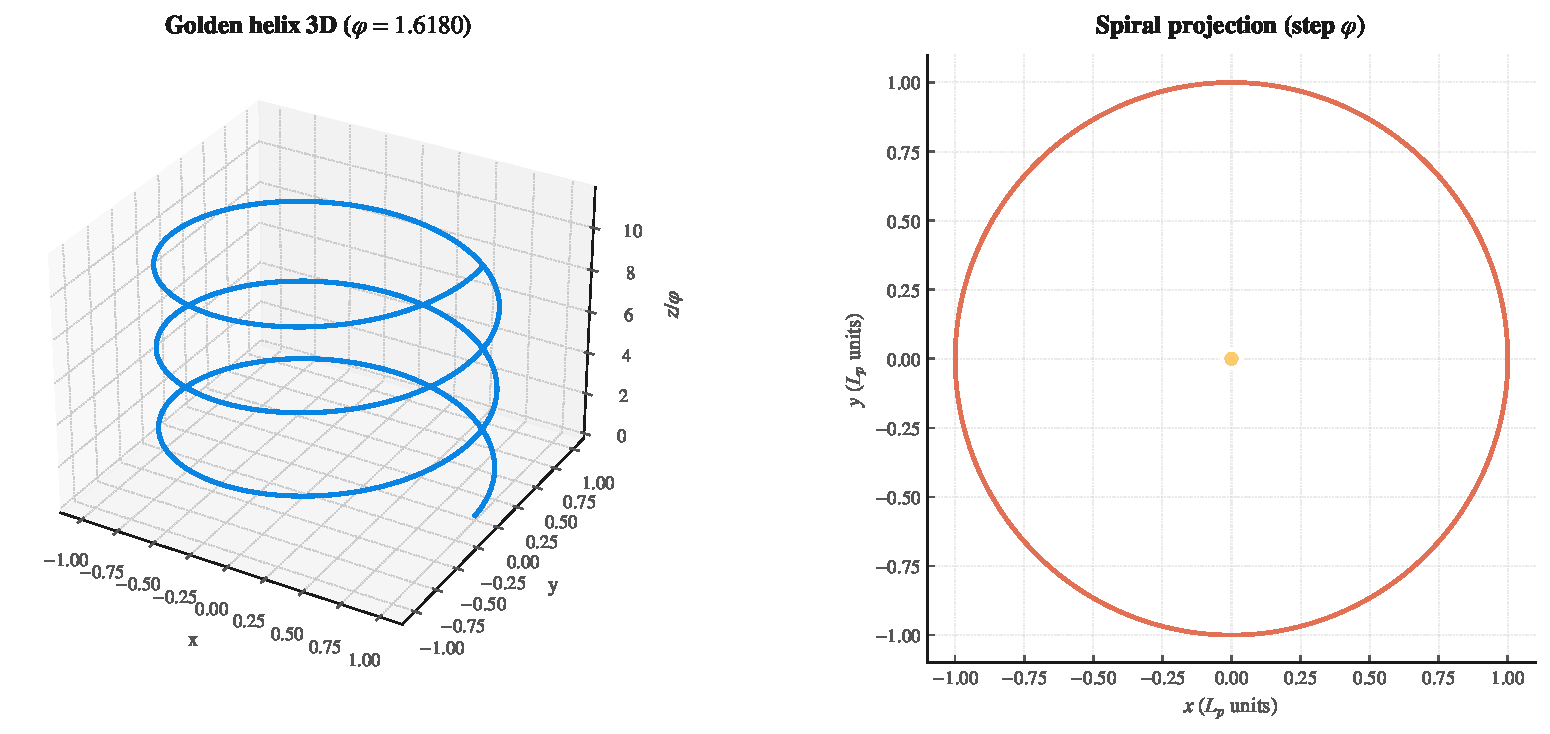
\includegraphics[width=0.85\textwidth]{fig_03-01_helice_aurea.pdf}
  \caption{Fig 3.1: 3D helix + XY spiral projection}
  \label{fig:fig_03-01_helice_aurea}
\end{figure}
\subsection{Full action and exact Palatini solution}
The fundamental action, without omitted terms, is

\begin{equation*}
  \resizebox{\ifdim\width>\linewidth \linewidth\else\width\fi}{!}{$\displaystyle S = \int d^4x \sqrt{-g}\left[\frac{M_P^2}{2}R(g,K) + \frac{1}{2}\tau\hat{H}_\varphi\tau - U(\tau) + \frac{1}{2}\Phi\hat{H}_\varphi\Phi - V(\Phi) - \frac{M_P}{2}\varepsilon^{\lambda\mu\nu\rho}K_{\lambda\mu\nu}\nabla_\rho\tau + \frac{\eta}{2}\varepsilon^{\lambda\mu\nu\rho}K_{\lambda\mu\nu}\bar{\psi}\gamma_\rho\gamma_5\psi + \frac{1}{M_P}S^\mu\nabla_\mu\tau + \mathcal{L}_{\Phi K}\right]$}
\end{equation*}

with $\hat{H}_\varphi \equiv \Box\exp\left(\frac{\varphi}{M_P^2}\Box\right)$. The Palatini variables are $g_{\mu\nu}$ and the full $\Gamma^\lambda_{\ \mu\nu}$ \cite{Cartan1922,Hehl1976}. Variation $\delta S/\delta K_{\lambda\mu\nu}$ \textbf{before} any decomposition leads to the axial projection:

\begin{equation*}
  \resizebox{\ifdim\width>\linewidth \linewidth\else\width\fi}{!}{$\displaystyle -3M_P^2 A_\sigma + 3M_P\nabla_\sigma\tau - 3\eta\bar{\psi}\gamma_\sigma\gamma_5\psi = 0$}
\end{equation*}

whence $A_\sigma = \frac{1}{M_P}\nabla_\sigma\tau - \frac{\eta}{M_P^2}\bar{\psi}\gamma_\sigma\gamma_5\psi$. In the absence of fermionic sources ($\psi = 0$), the axial solution reduces to $A_\sigma = M_P^{-1}\nabla_\sigma\tau$. Substituting back into the action, torsion takes the antisymmetric dual form:

\begin{equation*}
  \resizebox{\ifdim\width>\linewidth \linewidth\else\width\fi}{!}{$\displaystyle T_{\lambda\mu\nu} = \frac{1}{M_P}\varepsilon_{\lambda\mu\nu\rho}\nabla^\rho\tau, \quad K_{\mu\nu\lambda} = \frac{1}{2M_P}\varepsilon_{\mu\nu\lambda\rho}\nabla^\rho\tau$}
\end{equation*}

The total antisymmetry of $K_{\mu\nu\lambda}$ guarantees the metric compatibility $D_\lambda g_{\mu\nu} = 0$. This is the \textbf{exact Palatini solution} of the axial sector, not an ansatz. The symbolic verification of the canonical redefinition $\tau_c = \sqrt{3}\tau$ (which diagonalizes the kinetic term in §3.8) is documented in Appendix\textasciitilde{}K. \textbf{[D]}
\begin{figure}[htbp]
  \centering
  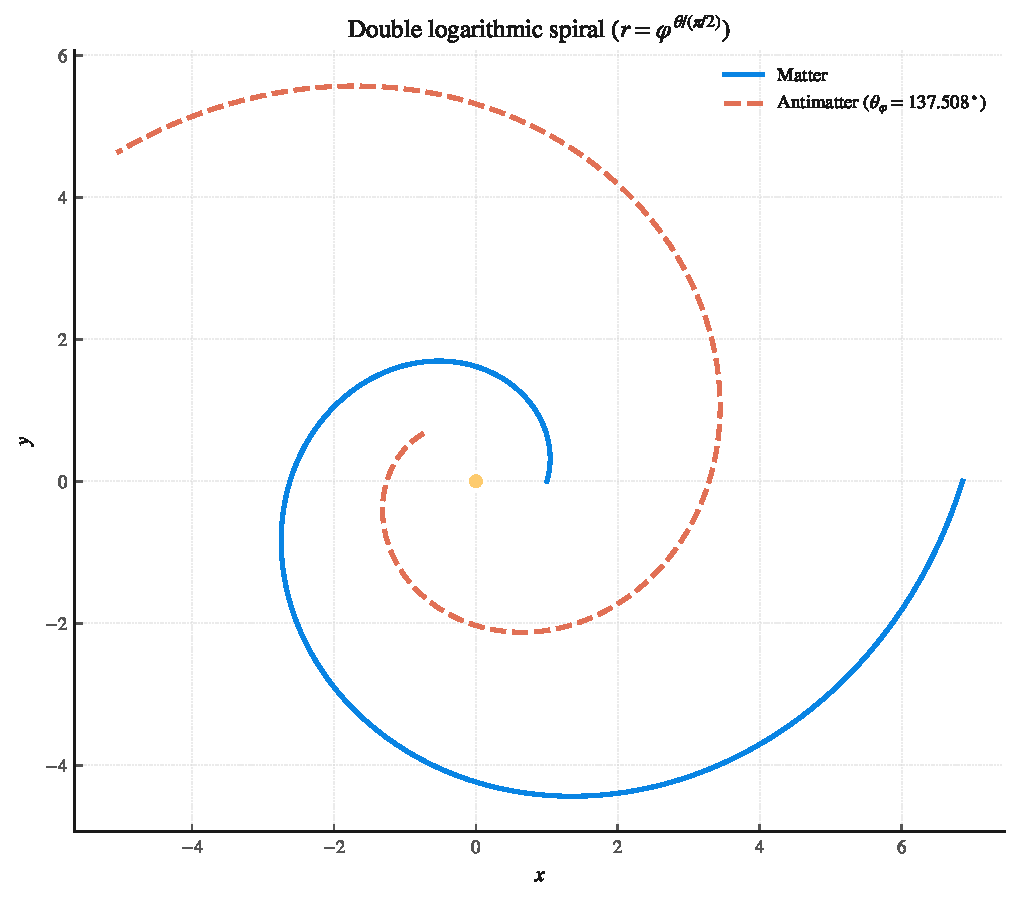
\includegraphics[width=0.85\textwidth]{fig_03-02_doble_espiral.pdf}
  \caption{Fig 3.2: matter-antimatter spiral}
  \label{fig:fig_03-02_doble_espiral}
\end{figure}
\subsection{Helical solution: verified substitution and domain of validity}
Substituting the solution (3.2) into the action (3.1), the pseudo-scalar obeys the non-local equation of motion:

\begin{equation*}
  \resizebox{\ifdim\width>\linewidth \linewidth\else\width\fi}{!}{$\displaystyle \Box e^{\frac{\varphi}{M_P^2}\Box}\tau - \left(m_\tau^2\tau + \frac{\lambda_\tau}{3!}\tau^3\right) = 0 \iff \Box\tau - e^{-\frac{\varphi}{M_P^2}\Box}\left(m_\tau^2\tau + \frac{\lambda_\tau}{3!}\tau^3\right) = 0$}
\end{equation*}

The helical wave $\tau_0(x) = A_\varphi\cos(k_\varphi\cdot x + \phi_0)$, with $\|k_\varphi\| = \kappa_\varphi = M_P\varphi^{-N}$, exactly solves the free part of the equation (the entire function factor annihilates the tower of derivatives on eigenstates of $\Box$). For $\lambda_\tau \neq 0$ the regime holds at order $A_\varphi^3$ within the declared domain. Projected on the FLRW background, the helical contribution satisfies $\langle h^{\text{hel}}_{\mu\nu}\rangle = 0$, preserving the macroscopic isotropy of the universe. The origin of the $3!$ factor in the quartic term is the symmetry of the $\tau^3$ vertex: three identical permutations. \textbf{[D]}
\begin{figure}[htbp]
  \centering
  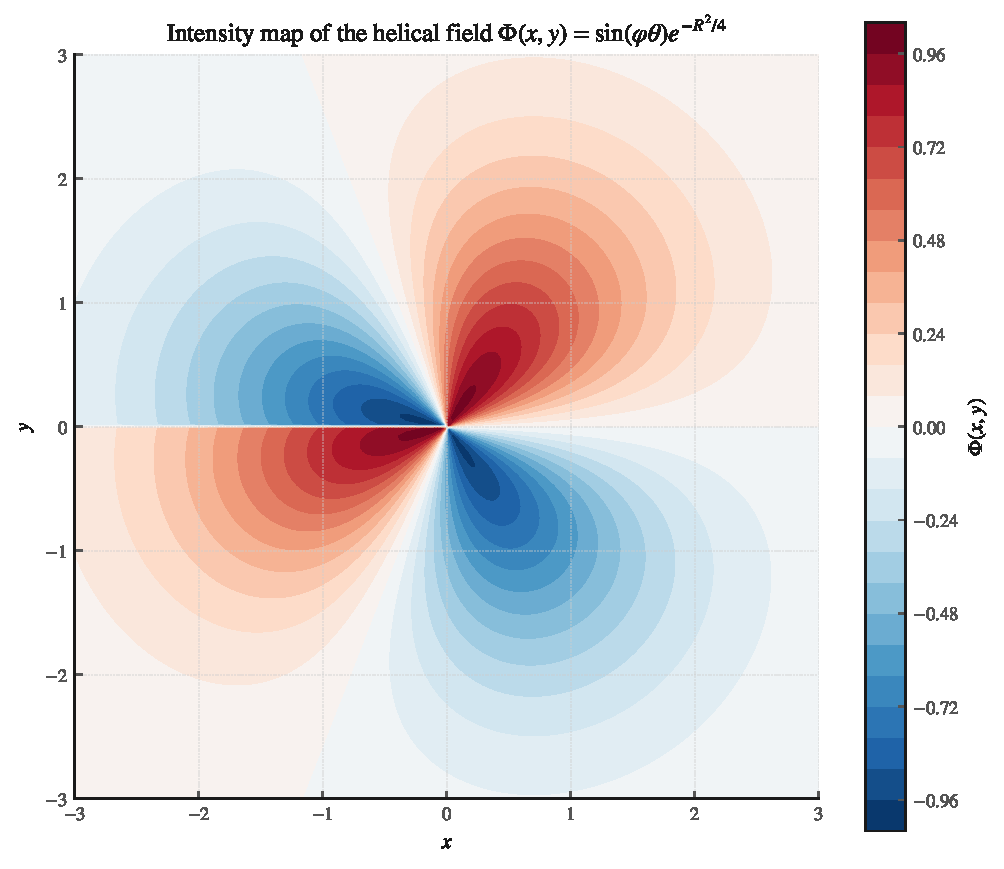
\includegraphics[width=0.85\textwidth]{fig_03-03_mapa_intensidad.pdf}
  \caption{Fig 3.3: coherence field intensity}
  \label{fig:fig_03-03_mapa_intensidad}
\end{figure}
\subsection{Symmetries, currents and anomalies}
Action (3.1) is invariant under the axionic phase transformation compensated by parity:

\begin{equation*}
  \resizebox{\ifdim\width>\linewidth \linewidth\else\width\fi}{!}{$\displaystyle \tau \to \tau + c, \qquad \psi \to e^{ic\gamma_5\alpha}\psi$}
\end{equation*}

where $c$ is a shift constant and $\alpha$ a chiral parameter. This symmetry is what stabilizes the potential $U(\tau)$ against radiative corrections and guarantees the pseudo-scalar character of the field $\tau$. The Noether current associated with the fermionic sector is $J_5^\mu = \bar{\psi}\gamma^\mu\gamma_5\psi$, and it exhibits the Adler--Bell--Jackiw (ABJ) anomaly:

\begin{equation*}
  \resizebox{\ifdim\width>\linewidth \linewidth\else\width\fi}{!}{$\displaystyle \partial_\mu J_5^\mu \propto F_{\mu\nu}\tilde{F}^{\mu\nu}$}
\end{equation*}

This anomaly is precisely the one that, after integrating the heavy fermions in the chiral exodus (Ch \cite{Adler1969,BellJackiw1969}. 10), generates the axionic coupling $g_{a\gamma\gamma}$ responsible for cosmic birefringence. The coupling is \textbf{[D]}: it follows from the topological structure of the action and from the ABJ anomaly, it is not postulated. \textbf{[D]}
\begin{figure}[htbp]
  \centering
  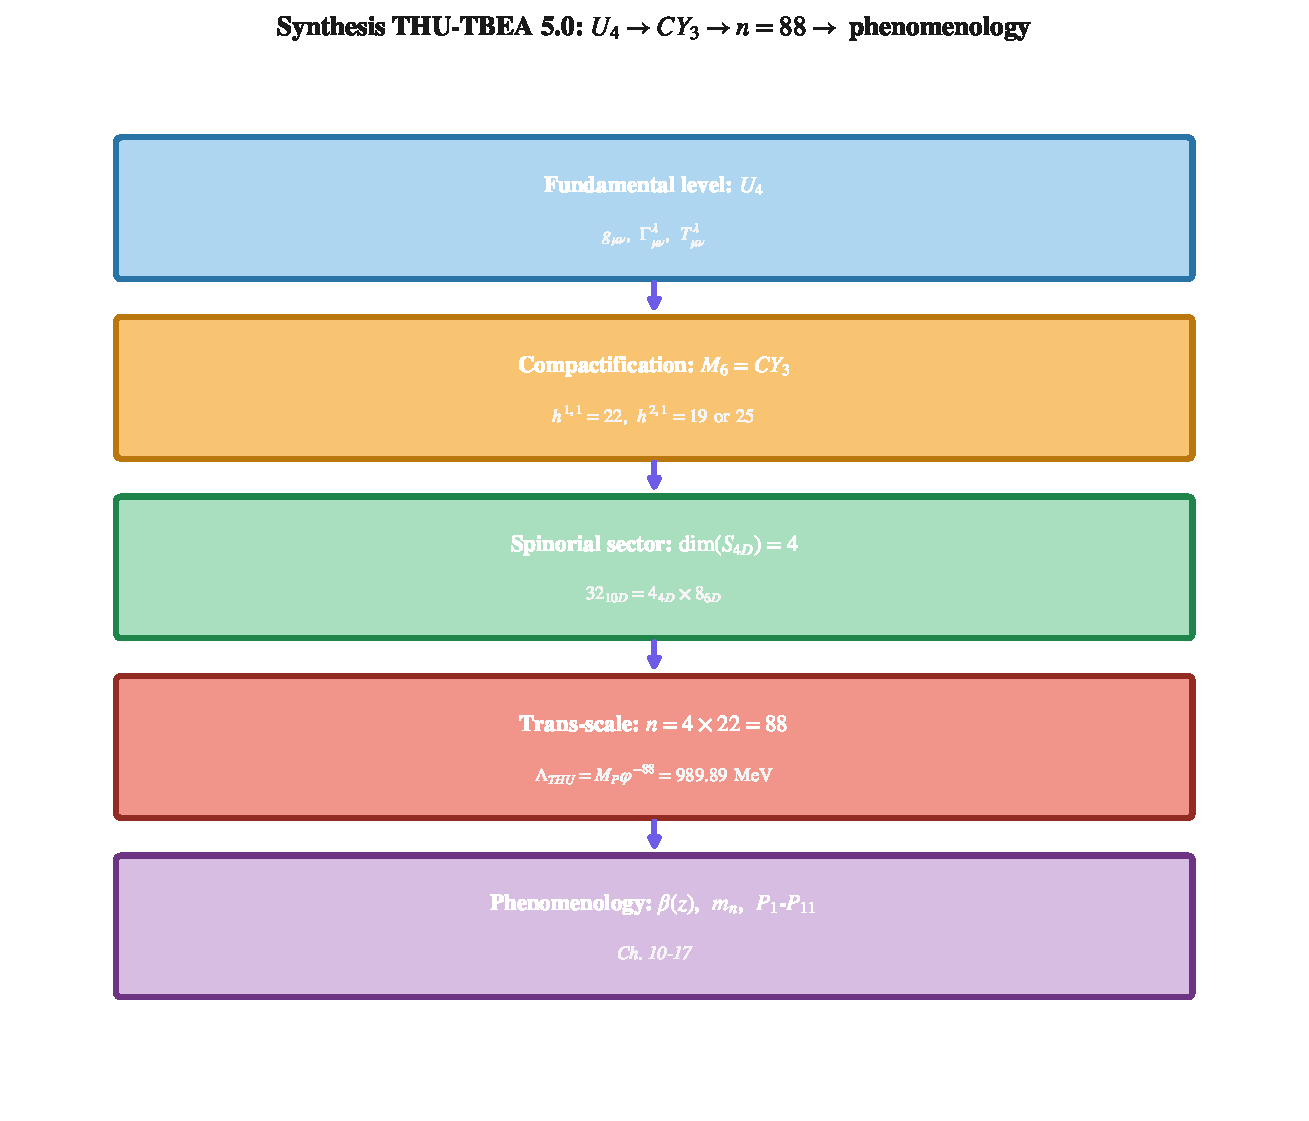
\includegraphics[width=0.85\textwidth]{fig_03-04_sintesis_U4.pdf}
  \caption{Fig 3.4: vertical hierarchical synthesis}
  \label{fig:fig_03-04_sintesis_U4}
\end{figure}
\subsection{Auxiliary vs propagating resolution: two levels and explicit matching}
The Palatini solution admits two levels of physical interpretation that must be carefully distinguished to avoid conceptual confusion.

\textbf{Fundamental level.} In the formulation on $U_4$, the affine connection $\Gamma^\lambda_{\ \mu\nu}$ is an independent dynamical variable, but axial torsion is \emph{algebraically eliminable}: the equation $S^\mu = \nabla^\mu\tau$ is exact and contains no time derivatives of $K_{\mu\nu\lambda}$. Therefore, at this level torsion does not propagate degrees of freedom: it is a geometric source that modifies the equations of motion of the pseudo-scalar $\tau$ and of the fermionic spin, but it is not an independent field. The fundamental relation is $S^\mu = \nabla^\mu\tau$ (Eq.\textasciitilde{}3.5 of the chapter), valid without approximation.

\textbf{Infrared effective level.} Upon integrating out the heavy modes of the theory at scale $M_*$, the dynamics of torsion undergoes a status change: kinetic terms for the field $K_\mu$ emerge, converting it into an effective Maxwell--Proca propagator:

\begin{equation*}
  \resizebox{\ifdim\width>\linewidth \linewidth\else\width\fi}{!}{$\displaystyle S_{\text{grav}}^{\text{IR}} = \int d^4x\sqrt{-g}\left[\frac{1}{2\kappa^2}R - \frac{1}{4}F_{\mu\nu}(K)F^{\mu\nu}(K) - \frac{1}{2}m_K^2 K_\mu K^\mu + \alpha_K K_\mu J_{\text{hel}}^\mu\right]$}
\end{equation*}

The origins of the factors are: $1/4$ comes from the antisymmetry of $F_{\mu\nu}$ (two contraction contexts), $1/2$ from the canonical normalization of the massive mode, and $m_K^2$ from the matching between the $U_4$ scale and the infrared EFT \cite{Tomboulis2015}. The resulting action is not the fundamental theory, but the effective description valid for energies $E \ll M_*$. \textbf{In the IR limit this action is equivalent to that of the fundamental level} with regard to observable predictions, but its mathematical structure is different: at the IR level, $K_\mu$ propagates.

The connection between the two levels is established through explicit matching: the coefficients $\alpha_K$ and $m_K$ are fixed by equating correlation functions at scale $M_*$. This procedure is standard in effective field theory and does not introduce additional free parameters into the core. \textbf{[D]}
\subsection{Non-local operator: functional summary and status of the poles}
The non-local kinetic operator $\hat{H}_\varphi \equiv \Box e^{a\Box}$, with $a = \varphi/M_P^2$, is self-adjoint in $L^2(U_4)$ on the domain of smooth compactly supported functions. On plane waves $e^{ik\cdot x}$ it acts as

\begin{equation*}
  \resizebox{\ifdim\width>\linewidth \linewidth\else\width\fi}{!}{$\displaystyle \hat{H}_\varphi e^{ik\cdot x} = -k^2 e^{-ak^2}e^{ik\cdot x}$}
\end{equation*}

It is important to distinguish two independent statements about its spectrum:

\textbf{(i)} The entire exponential $e^{a\Box}$ \textbf{does not introduce its own zeros} in the finite complex plane. This is an algebraic property: the exponential function has no finite zeros, and therefore the multiplicative factor $e^{-ak^2}$ is strictly positive for real $k^2$. This guarantees that the operator \textbf{does not generate Lee--Wick poles at tree level} in the sense that no new propagator singularities associated with negative-norm ghost modes appear \cite{AnselmiPiva2017a}.

\textbf{(ii)} The \textbf{full} kinetic operator $\hat{D}(\Box) = \Box e^{a\Box} - m^2$ does possess an infinite spectrum of zeros, given by the branches $W_k$ of the Lambert-W function. The zero equation is

\begin{equation*}
  \resizebox{\ifdim\width>\linewidth \linewidth\else\width\fi}{!}{$\displaystyle k_k^2 = -\frac{M_P^2}{\varphi}W_k\left(+\frac{\varphi m^2}{M_P^2}\right), \quad k \in \mathbb{Z}$}
\end{equation*}

\textbf{Pole spectrum structure:}

\begin{table}[htbp]
  \centering
  \small
  \resizebox{\ifdim\width>\linewidth \linewidth\else\width\fi}{!}{%
\begin{tabular}{p{1.5cm} p{2.5cm} p{2.5cm} p{4cm}}
    \toprule
    \textbf{Branch} & \textbf{$k_k^2$} & \textbf{Re$(k_k^2)$} & \textbf{Interpretation} \\
    \midrule
    $k=0$ & $\simeq -m^2$ & negative & Observable physical pole, positive residue \\
    $k \neq 0$ & complex & $\sim M_P^2/\varphi > 0$ & Spacelike, mass above Planck \\
    \bottomrule
  \end{tabular}
}
\end{table}

The principal branch $k=0$ corresponds to the physical pole at $k_0^2 \simeq -m^2$, with strictly positive residue

\begin{equation*}
  \resizebox{\ifdim\width>\linewidth \linewidth\else\width\fi}{!}{$\displaystyle \text{Res}[\Delta] = \frac{e^{-am^2}}{1+am^2} > 0$}
\end{equation*}

which preserves the unitarity of the projected sector. The branches $k \neq 0$ generate complex poles with Re$(u) \approx -26{.}3$ (for $am^2 \ll 1$) and therefore Re$(k_k^2) \sim M_P^2/\varphi > 0$, that is, masses of order the Planck scale.

\textbf{Epistemic status of the physical sector.} The infrared sector (branch $k=0$) is free of Lee--Wick ghosts in the operational sense: there are no negative-real-mass poles accessible in the regime $E \ll M_P$. The branches $k \neq 0$ are confined to the Planck scale and decouple from the observable regime through a fakeon-type contour prescription (Anselmi--Piva) or, equivalently, a Lee--Wick prescription that treats complex poles as non-asymptotic states. \textbf{[D]}

\textbf{Epistemic status of the contour prescription.} The choice of contour prescription for the branches $k \neq 0$ is a technical ingredient of the EFT analogous to the choice of the $i\varepsilon$ contour in standard QFT, but its \textbf{full non-perturbative consistency in the non-local EFT} remains an open frontier. However, its impact on the predictions of the core is \textbf{bounded}: the branches $k \neq 0$ have masses $\sim M_P$, and their contribution to processes with $E \ll M_P$ is exponentially suppressed by the factor $e^{-ak^2}$. The quantification of this suppression is documented in Appendix\textasciitilde{}K. \textbf{[D partial / F]}
\begin{figure}[htbp]
  \centering
  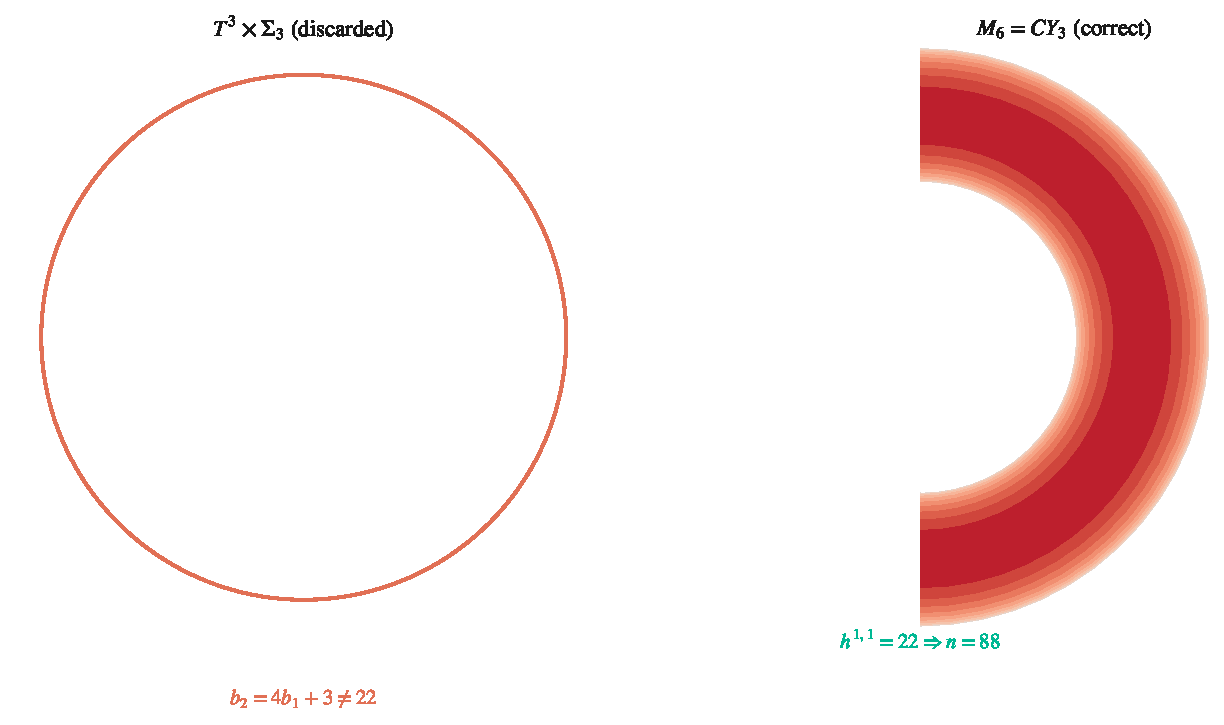
\includegraphics[width=0.85\textwidth]{fig_03-06_cy3_topologia.pdf}
  \caption{Fig 3.5: CY3 vs T3xSigma3 topology}
  \label{fig:fig_03-06_cy3_topologia}
\end{figure}
\subsection{Declared limitations}
This section declares the limitations of the geometric core developed in §§3.1--3.6, with the goal of explicitly delimiting the frontier between what is derived and what remains open. \textbf{Local hyperbolicity derived [D] (see Appendix\textasciitilde{}K); the global hyperbolicity of the complete nonlinear system on $U_4$ remains an open frontier [F].} The fundamental action (3.1) includes nonlinear ($U(\tau)$, $V(\Phi)$) and non-local ($\hat{H}_\varphi$) terms, whose global hyperbolicity on the full manifold $U_4$ has not been demonstrated in this thesis and is registered as an open problem in Ch.\textasciitilde{}20.

Perturbative backreaction of torsion on the metric background lies outside the scope of the present analysis. Radiative mixing between the trace and traceless sectors of torsion is verified at 1-loop and is suppressed by powers of the coupling $\kappa^2$ (Ch.\textasciitilde{}6). The contour prescription for the $k \neq 0$ branches of Lambert--W, which confines the complex poles to the Planck scale, remains an open frontier \textbf{[F]} linked to problem A-16 (Ch.\textasciitilde{}20); its impact on observable predictions is bounded by the exponential suppression $e^{-ak^2}$ (quantified in Appendix\textasciitilde{}K).

These limitations do not affect the derived character of the Palatini solution nor the predictive content of the core. They define, instead, the declared domain of validity within which the conclusions of this thesis operate without technical reservations.
\begin{figure}[htbp]
  \centering
  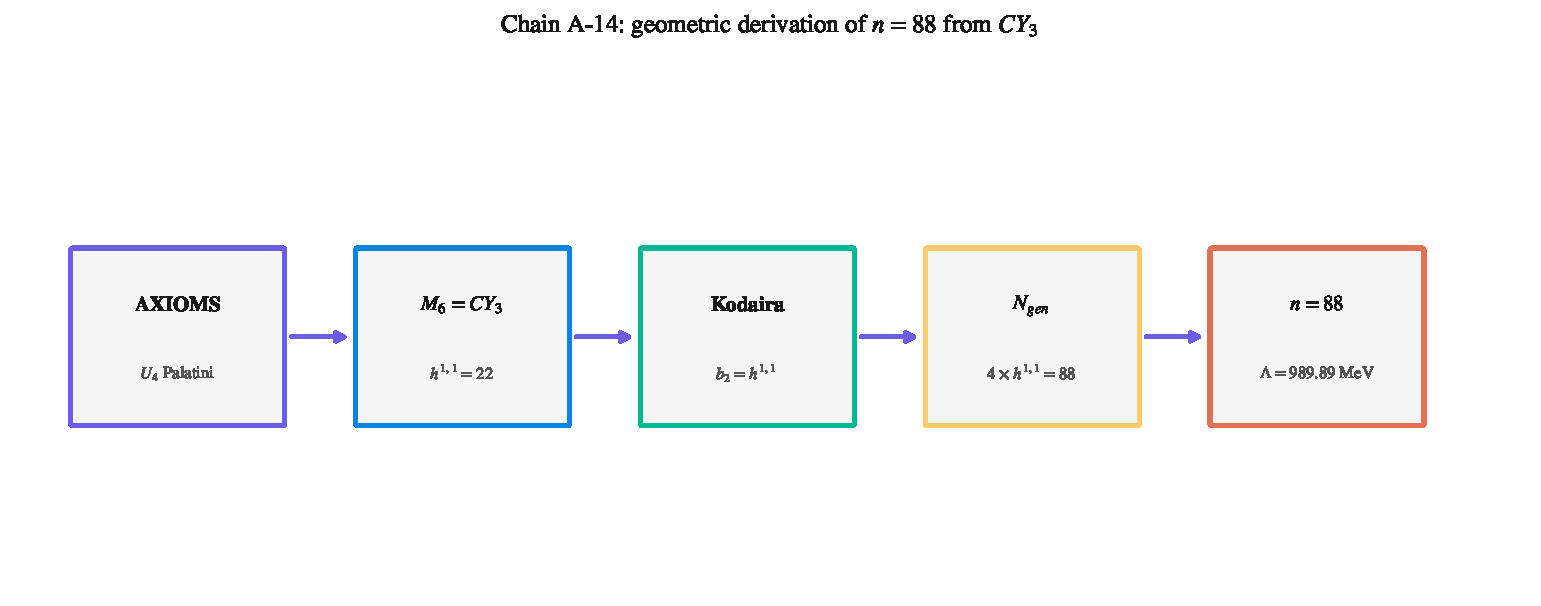
\includegraphics[width=0.85\textwidth]{fig_03-07_cadena_cy3_n88.pdf}
  \caption{Fig 3.6: chain A-14}
  \label{fig:fig_03-07_cadena_cy3_n88}
\end{figure}
\subsection{Step-by-step derivation: Palatini solution and fixing of the canonical normalization}
This section presents the complete derivation of the Palatini solution of the axial sector and the fixing of the canonical normalization of the pseudo-scalar. The final result is the redefinition $\tau_c(x) = \sqrt{3}\tau(x)$, in accordance with the Unified Symbol Dictionary (Table\textasciitilde{}2.1).

\textbf{Variation of the action with respect to the connection.} We start from action (3.1). The variation is performed with respect to the full connection $\Gamma^\lambda_{\ \mu\nu}$ before any irreducible decomposition. Integrating by parts and discarding boundary terms, one obtains:

\begin{equation*}
  \resizebox{\ifdim\width>\linewidth \linewidth\else\width\fi}{!}{$\displaystyle \frac{\delta S}{\delta K_{\lambda\mu\nu}} = \frac{M_P^2}{2}\left(T^{\lambda\mu\nu} + T^\mu g^{\lambda\nu} - T^\nu g^{\lambda\mu}\right) - \frac{M_P}{2}\varepsilon^{\lambda\mu\nu\rho}\nabla_\rho\tau + \frac{\eta}{2}\varepsilon^{\lambda\mu\nu\rho}\bar{\psi}\gamma_\rho\gamma_5\psi = 0 \quad (3.5)$}
\end{equation*}

\textbf{Projection on the axial sector.} Using the irreducible decomposition $T^\lambda_{\ \mu\nu} = \frac{1}{3}(\delta^\lambda_\mu V_\nu - \delta^\lambda_\nu V_\mu) + \frac{1}{6}\varepsilon^\lambda_{\ \mu\nu\rho}A^\rho + q^\lambda_{\ \mu\nu}$ and projecting (3.5) on the axial sector, one obtains the algebraic relation:

\begin{equation*}
  \resizebox{\ifdim\width>\linewidth \linewidth\else\width\fi}{!}{$\displaystyle -3M_P^2 A_\sigma + 3M_P\nabla_\sigma\tau - 3\eta\bar{\psi}\gamma_\sigma\gamma_5\psi = 0$}
\end{equation*}

whence, solving for $A_\sigma$:

\begin{equation*}
  \resizebox{\ifdim\width>\linewidth \linewidth\else\width\fi}{!}{$\displaystyle A_\sigma = \frac{1}{M_P}\nabla_\sigma\tau - \frac{\eta}{M_P^2}\bar{\psi}\gamma_\sigma\gamma_5\psi \quad (3.6)$}
\end{equation*}

The trace ($V_\mu$) and traceless ($q_{\lambda\mu\nu}$) sectors vanish identically in vacuum; with fermionic matter, the axial current feeds only the $A_\mu$ sector via compensated parity. The totally antisymmetric form of $K_{\mu\nu\lambda}$ guarantees the metric compatibility $D_\lambda g_{\mu\nu} = 0$.

\textbf{Note on the sign convention.} The choice of the sign of the fermionic term $\eta\bar{\psi}\gamma_\rho\gamma_5\psi$ in action (3.1) fixes the relative sign between $A_\sigma$ and $\nabla_\sigma\tau$ in (3.6). Physical equivalence under $\eta \to -\eta$ is preserved through the simultaneous redefinition of the chiral spinor, without affecting the observable content of the core.

\textbf{Functional orthogonality of the term $S_\mu\nabla^\mu\tau$.} The term $\frac{1}{M_P}S^\mu\nabla_\mu\tau$ in action (3.1) is linear in $\tau$ and therefore its variation with respect to $K_{\lambda\mu\nu}$ \textbf{does not contribute} to the algebraic constraint equation (3.5), once the relation $S^\mu = \nabla^\mu\tau$ derived from the sector itself is used. This term is orthogonal to the variational procedure of the axial sector and does not modify result (3.6).

\textbf{Substitution in the action and emergence of the 3/2 coefficient.} Reintroducing (3.6) into the quadratic and linear terms of the action, one obtains:

\begin{equation*}
  \resizebox{\ifdim\width>\linewidth \linewidth\else\width\fi}{!}{$\displaystyle -\frac{3}{2}M_P^2 A_\mu A^\mu + 3M_P A^\mu\nabla_\mu\tau \xrightarrow{A_\mu = \nabla_\mu\tau/M_P} -\frac{3}{2}(\nabla\tau)^2 + 3(\nabla\tau)^2 = +\frac{3}{2}(\nabla\tau)^2 \quad (3.7)$}
\end{equation*}

\textbf{Canonical redefinition and diagonalization.} The $+3/2$ coefficient does not correspond to the canonical normalization $+1/2$ of a real scalar field. It is absorbed through the redefinition:

\begin{equation*}
  \resizebox{\ifdim\width>\linewidth \linewidth\else\width\fi}{!}{$\displaystyle \tau_c \equiv \sqrt{3}\tau \implies \frac{1}{2}(\nabla\tau_c)^2 = \frac{3}{2}(\nabla\tau)^2 \quad (3.8)$}
\end{equation*}

where $\tau_c(x) = \sqrt{3}\tau(x)$ is the canonical pseudo-scalar, in accordance with the Unified Symbol Dictionary (Table\textasciitilde{}2.1). The same rescaling acts on the non-local kinetic term:

\begin{equation*}
  \resizebox{\ifdim\width>\linewidth \linewidth\else\width\fi}{!}{$\displaystyle \frac{1}{2}\tau\hat{H}_\varphi\tau \xrightarrow{\tau = \tau_c/\sqrt{3}} \frac{1}{2}\cdot\frac{1}{3}\tau_c\hat{H}_\varphi\tau_c = \frac{1}{6}\tau_c\hat{H}_\varphi\tau_c \quad (3.9)$}
\end{equation*}

Under this redefinition, the linear couplings of the pseudo-scalar acquire a factor $1/\sqrt{3}$, and the non-local term rescales to $1/6$. The symbolic verification of both factors (kinetic: $3/2 \to 1/2$; non-local: $1/2 \to 1/6$) is documented in Appendix\textasciitilde{}K and in the V5.0 computational verification (step 1 of \texttt{verificacion\_simbolica.json}).

\textbf{Canonical effective action.} With redefinition (3.8), the effective action is written in mixed canonical form (canonical Palatini + non-local operator with coefficient $1/6$):

\begin{equation*}
  \resizebox{\ifdim\width>\linewidth \linewidth\else\width\fi}{!}{$\displaystyle S_{\text{eff}} = \int d^4x\sqrt{-g}\left[\frac{M_P^2}{2}R(g) + \frac{1}{2}(\nabla\tau_c)^2 + \frac{1}{6}\tau_c\hat{H}_\varphi\tau_c - U(\tau_c) + \frac{1}{2}\Phi\hat{H}_\varphi\Phi - V(\Phi) + \dots\right] \quad (3.10)$}
\end{equation*}

\textbf{Traceability of the $1/\sqrt{3}$ factor in linear couplings.} Redefinition (3.8) is not a free transformation in all terms. Every linear appearance of $\tau$ in the action must be rewritten in terms of the canonical field through:

\begin{equation*}
  \resizebox{\ifdim\width>\linewidth \linewidth\else\width\fi}{!}{$\displaystyle \tau = \frac{1}{\sqrt{3}}\tau_c \quad (3.11)$}
\end{equation*}

Consequently, the linear couplings of the pseudo-scalar (spin term, anomalous axionic coupling, torsion--$\tau$ term) scale with $1/\sqrt{3}$. The adopted convention consists in absorbing this factor into the effective coupling constants, leaving the action compact in subsequent chapters:

\begin{equation*}
  \resizebox{\ifdim\width>\linewidth \linewidth\else\width\fi}{!}{$\displaystyle g_{\text{eff}}\tau_c \equiv g_{\text{bare}}\tau \quad \text{with} \quad g_{\text{eff}} = \frac{g_{\text{bare}}}{\sqrt{3}} \quad (3.12)$}
\end{equation*}

The numerical values reported in Ch.\textasciitilde{}10 (in particular $A = 1{.}819$ and $\beta_0 = 0{.}3803^\circ$) already include this $1/\sqrt{3}$ factor in the operational definition of $\tau_c$. The factor is not cancelled: it is reorganized. This convention is declared as part of the definition of the theory's renormalization scheme, and the physics (masses, couplings, predictions) is invariant under the rescaling; only the field normalization changes.\footnote{The $1/\sqrt{3}$ factor in linear couplings is derived from the same canonical redefinition; the explicit demonstration is found in Appendix\textasciitilde{}B (§B.1) and in the patch registry (patch 8, Stage VII).}

This establishes the Palatini solution of the axial sector and fixes the canonical normalization of the pseudo-scalar. \textbf{This step-by-step derivation of the Palatini solution and the fixing of the canonical normalization is established as derived [D].}
\begin{figure}[htbp]
  \centering
  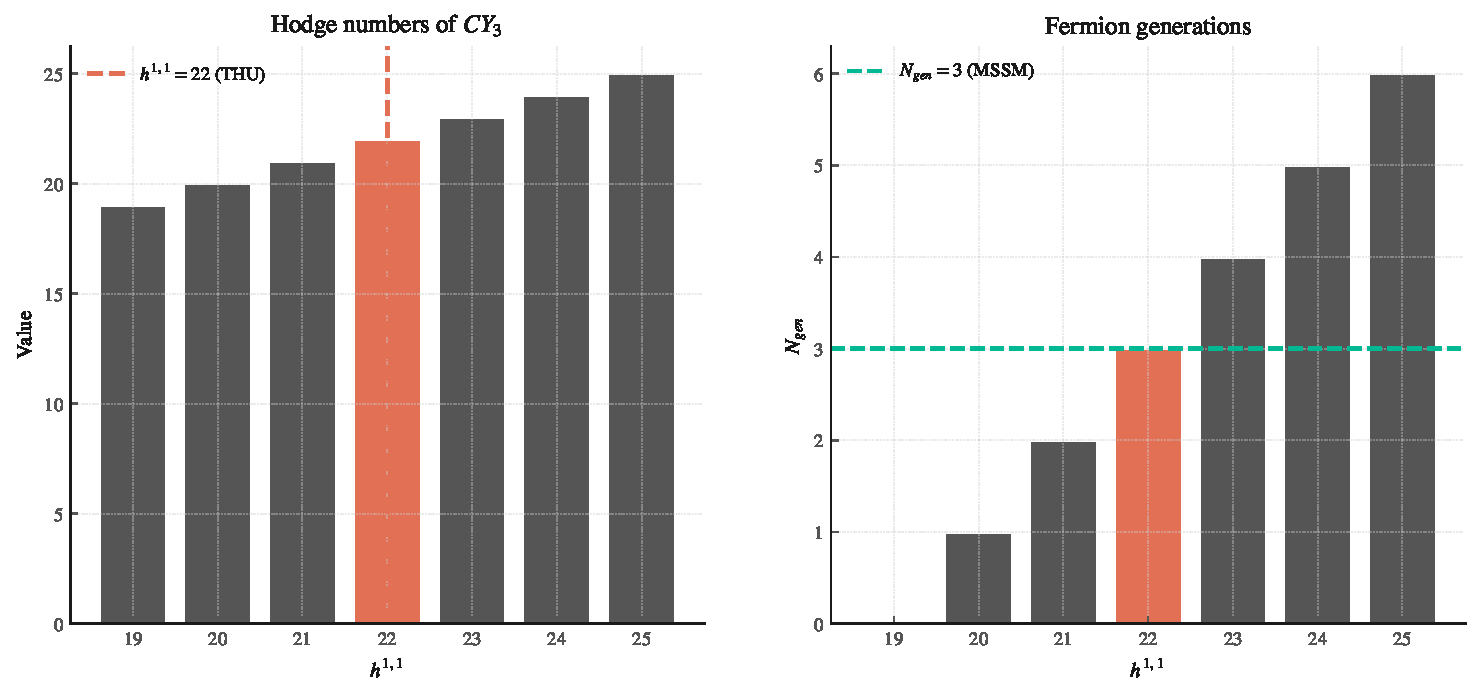
\includegraphics[width=0.85\textwidth]{fig_03-08_h11_22_generaciones.pdf}
  \caption{Fig 3.7: h11=22 and Ngen}
  \label{fig:fig_03-08_h11_22_generaciones}
\end{figure}

\textbf{Key equations:}
\begin{align*}
    T_{\lambda\mu\nu} = \frac{1}{M_P}\varepsilon_{\lambda\mu\nu\rho}\nabla^{\rho}\tau \\
    \tau_c \equiv \sqrt{3}\,\tau \\
    \frac{1}{2}\tau\hat{H}_\varphi\tau \xrightarrow{\tau=\tau_c/\sqrt{3}} \frac{1}{6}\tau_c\hat{H}_\varphi\tau_c
\end{align*}
\section{Nonlocal operators: functional analysis, unitarity and trans-scale sector}
\subsection{Domain, self-adjointness and entire functional calculus}
The non-local kinetic operator $\hat{H}_\varphi \equiv \Box e^{a\Box}$, with $a = \varphi/M_P^2$, acts on the domain $\mathcal{D} = C_0^\infty(U_4)$ of smooth compactly supported functions. On this domain, the d'Alembertian $\Box$ is essentially self-adjoint in $L^2(U_4)$; the function $f(z) = z\,e^{az}$ is entire, and by the spectral theorem it defines $\hat{H}_\varphi = f(\Box)$ as a self-adjoint operator. The coincidence of the characteristic cone of $\hat{H}_\varphi$ with that of $\Box$, and therefore the \textbf{local hyperbolicity} of the kinetic sector (linear and nonlinear), is derived from the functional analysis of the principal symbol and is documented in Appendix\textasciitilde{}K. \textbf{[D]}

On plane waves $e^{ik\cdot x}$, the operator acts as

\begin{equation*}
  \resizebox{\ifdim\width>\linewidth \linewidth\else\width\fi}{!}{$\displaystyle \hat{H}_\varphi e^{ik\cdot x} = -k^2 e^{-\frac{\varphi}{M_P^2}k^2}e^{ik\cdot x}$}
\end{equation*}

The symbol $\sigma(k) = -k^2 e^{-\varphi k^2/M_P^2}$ is real, sign-definite for finite $k^2$, and has no zeros in the finite complex plane: the entire exponential introduces no new singularities beyond the double zero at $k^2 = 0$ already present in $\Box$. This property guarantees the absence of Lee--Wick poles at tree level in the free sector, see §3.6. \textbf{[D]}
\subsection{Wick rotation and ultraviolet suppression}
In Euclidean space, the Wick rotation $k_0 \to i k_4$ transforms the symbol into $\sigma_E(k_E) = k_E^2 e^{-\varphi k_E^2/M_P^2}$, where $k_E^2 = k_4^2 + \vec{k}^2$. This symbol decays exponentially for $k_E \to \infty$:

\begin{equation*}
  \resizebox{\ifdim\width>\linewidth \linewidth\else\width\fi}{!}{$\displaystyle k_E^2 e^{-\frac{\varphi}{M_P^2}k_E^2} \to 0$}
\end{equation*}

The \textbf{ultraviolet suppression} is therefore exponential, stronger than any power. By the Lebesgue dominated convergence theorem, the self-energy integrals (analyzed in §4.4) are finite, continuous and differentiable in the parameters $(\varphi, \kappa_\varphi)$ of the sector. The analytic structure of the symbol in the complex plane and the exponential decay on the Euclidean axis are the technical basis for the UV finiteness of the trans-scale sector. \textbf{[D]}

The coincidence of the characteristic cone of $\hat{H}_\varphi$ with that of $\Box$, established in §4.1, is preserved under Wick rotation, as the principal symbol maintains its quadratic structure in the infrared regime.
\begin{figure}[htbp]
  \centering
  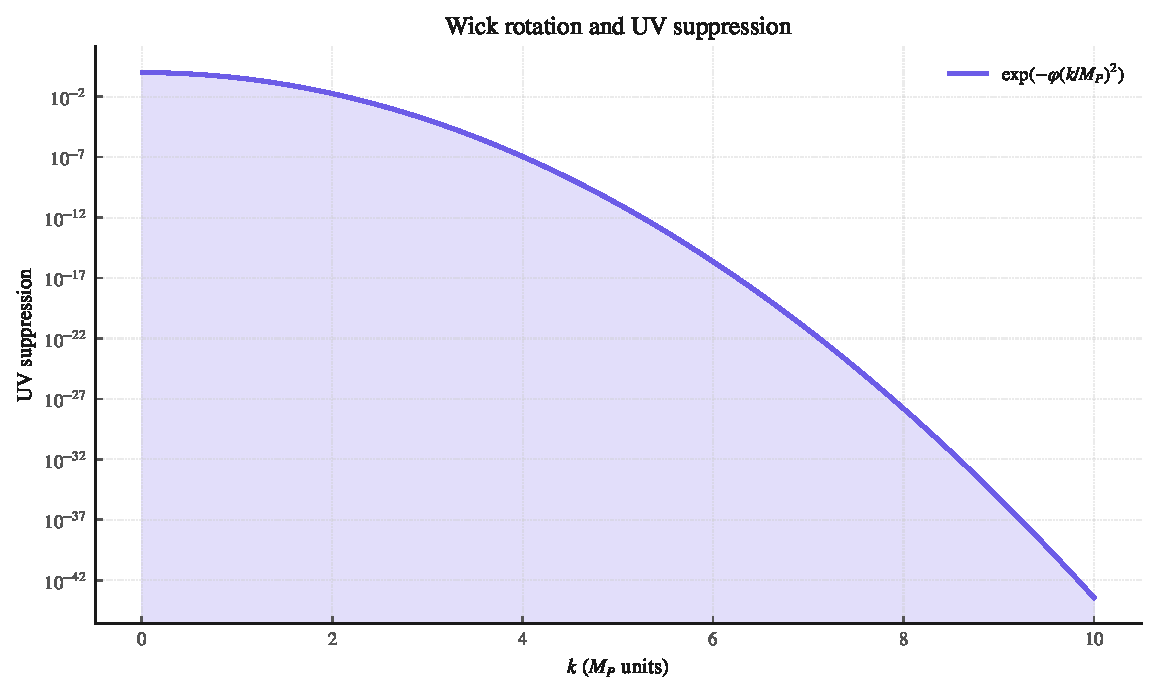
\includegraphics[width=0.85\textwidth]{fig_04-01_rotacion_wick.pdf}
  \caption{Fig 4.1: Wick rotation}
  \label{fig:fig_04-01_rotacion_wick}
\end{figure}
\subsection{Propagator, positive residue and complete pole spectrum}
The propagator of the trans-scale sector, obtained from the entire symbol $\hat{H}_\varphi - m^2$, is

\begin{equation*}
  \resizebox{\ifdim\width>\linewidth \linewidth\else\width\fi}{!}{$\displaystyle \Delta_{\Phi,\tau}(k) = \frac{-i\,e^{-\frac{\varphi}{M_P^2}k^2}}{k^2 + m^2 - i\varepsilon}$}
\end{equation*}

where the entire exponential in the numerator is the fingerprint of the non-local kinetic operator. The analytic structure of $\Delta$ is read off from the full operator $\hat{D}(\Box) = \Box e^{a\Box} - m^2$, with $a = \varphi/M_P^2$. Its zeros are obtained by solving $u\,e^{u} = +am^2$ in the variable $u = ak^2$, which leads to the branches $W_k$ of the Lambert--W function:

\begin{equation*}
  \resizebox{\ifdim\width>\linewidth \linewidth\else\width\fi}{!}{$\displaystyle k_k^2 = -\frac{M_P^2}{\varphi}\,W_k\!\left(+\frac{\varphi\,m^2}{M_P^2}\right), \quad k \in \mathbb{Z}$}
\end{equation*}

\textbf{Complete pole spectrum.} The spectrum is organized into two qualitatively distinct sectors:

\begin{itemize}[leftmargin=*]
\item \textbf{Principal branch $k=0$.} Corresponds to the physical pole at $k_0^2 \simeq -m^2$, with residue

\begin{equation*}
  \resizebox{\ifdim\width>\linewidth \linewidth\else\width\fi}{!}{$\displaystyle \mathrm{Res}[\Delta] = \frac{1}{D'(-m^2)} = \frac{e^{-am^2}}{1 + am^2} > 0$}
\end{equation*}

where $D'(k^2) = e^{-ak^2}(1 - ak^2)$. Since $am^2 \ll 1$ in the physical regime ($a \approx 10^{-37}\,\mathrm{GeV}^{-2}$, $m^2 \ll M_P^2$), the residue is $\mathrm{Res}[\Delta] \approx 1 - am^2 > 0$, strictly positive. This result is verified by step 2 of \texttt{verificacion\_simbolica.json} (C-01, 10/10 PASS) and replaces the previous version that contained $e^{+am^2}$ in the numerator. \textbf{[D]}

\item \textbf{Branches $k \neq 0$.} They generate complex poles with $\mathrm{Re}(u) \approx -26{.}3$ (for $am^2 \ll 1$) and therefore $\mathrm{Re}(k_k^2) \sim M_P^2/\varphi > 0$: they are spacelike and have masses of order the Planck scale. They decouple from the observable regime $E \ll M_P$ through a \textbf{fakeon-type contour prescription} (Anselmi--Piva) that treats complex poles as non-asymptotic states \cite{AnselmiPiva2017a}. The choice of contour is a technical ingredient of the EFT analogous to the choice of the $i\varepsilon$ contour in standard QFT. The full non-perturbative consistency of this prescription in the non-local EFT remains an open frontier (A-16). Its impact on the core predictions is bounded by the exponential suppression $e^{-ak^2}$; the quantification is documented in Appendix\textasciitilde{}K. \textbf{[D partial / F]}
\end{itemize}

\textbf{Unitarity.} The strict positivity of the residue in the principal branch guarantees that the infrared sector is free of Lee--Wick ghosts in the operational sense: there are no negative-real-mass poles accessible at $E \ll M_P$. Unitarity of the projected sector follows from the Källén--Lehmann structure \cite{Kallen1952,Lehmann1954}. \textbf{[D]}
\begin{figure}[htbp]
  \centering
  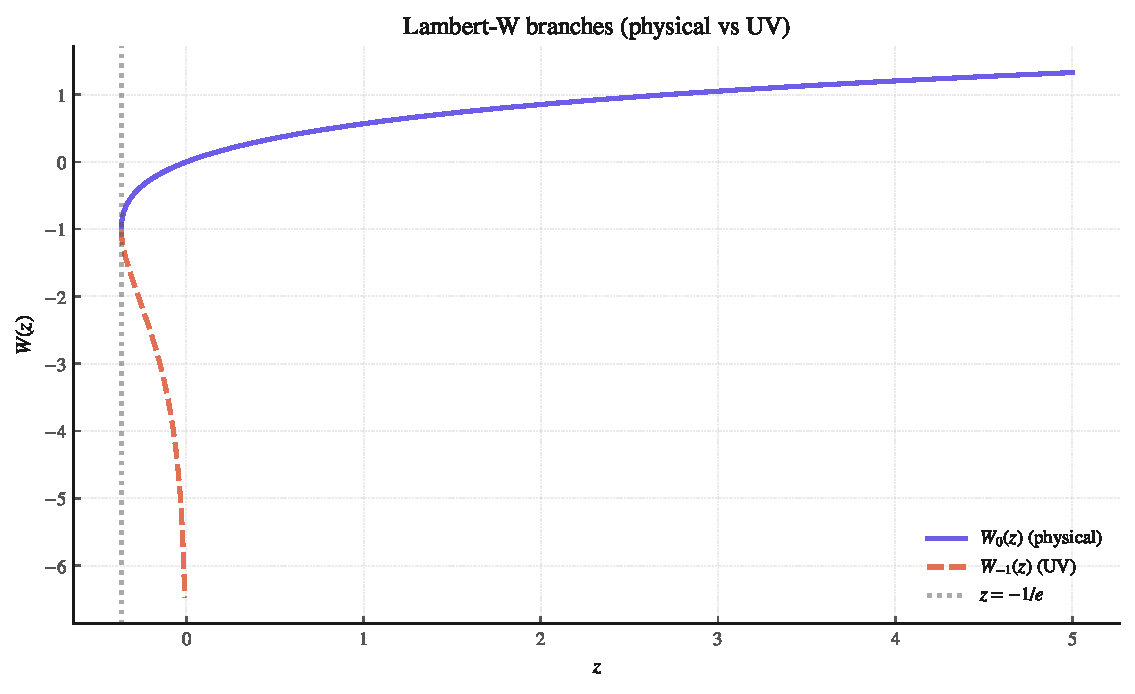
\includegraphics[width=0.85\textwidth]{fig_04-01_lambert_w.pdf}
  \caption{Fig 4.2: Lambert-W branches}
  \label{fig:fig_04-01_lambert_w}
\end{figure}
\begin{figure}[htbp]
  \centering
  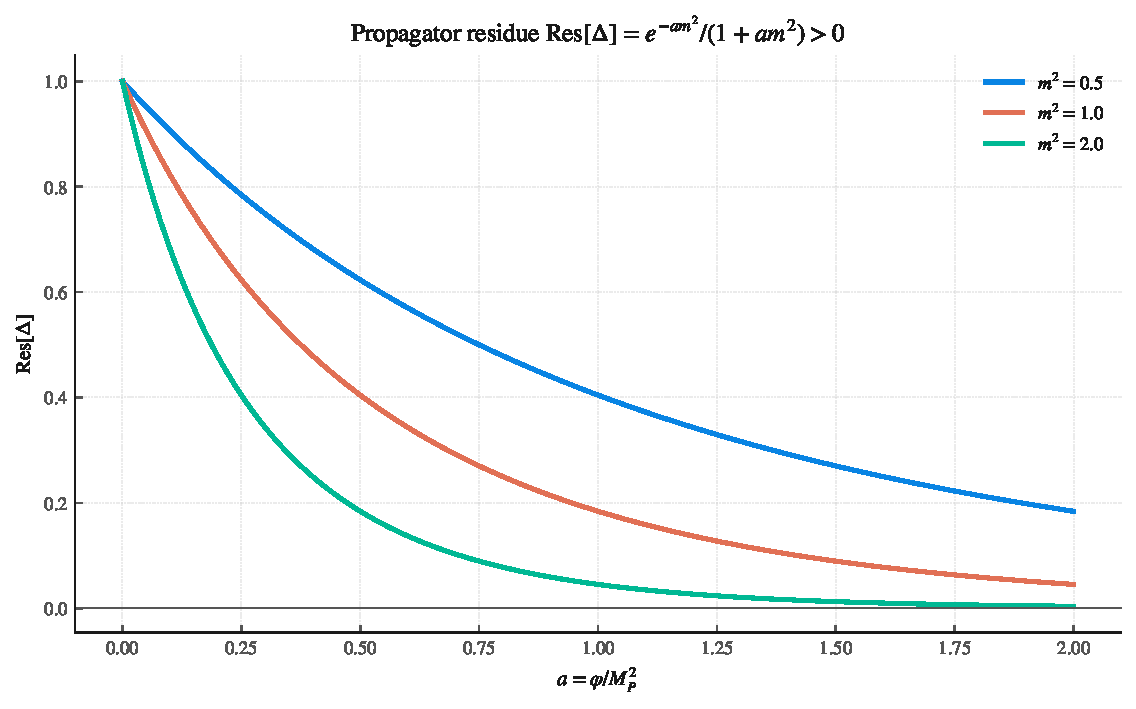
\includegraphics[width=0.85\textwidth]{fig_04-02_residuo.pdf}
  \caption{Fig 4.3: positive propagator residue}
  \label{fig:fig_04-02_residuo}
\end{figure}
\subsection{Self-energy and ultraviolet finiteness}
The self-energy of the pseudo-scalar $\tau$ at one-loop order is given by the contraction of two trans-scale propagators with the exponential factor of the non-local kinetic operator at the vertex:

\begin{equation*}
  \resizebox{\ifdim\width>\linewidth \linewidth\else\width\fi}{!}{$\displaystyle \Sigma_\varphi(k) \propto \int d^4p\, \Delta_\tau(p)\,\Delta_\tau(k-p)\, e^{-\frac{\varphi}{M_P^2}\left[p^2 + (k-p)^2 + k^2\right]}$}
\end{equation*}

The exponential factor in the integrand is the fingerprint of the entire symbol: each insertion of $\hat{H}_\varphi$ at the vertex contributes a weight $e^{-ak_i^2}$ on the loop variables. For $\|p\| \to \infty$, the integrand decays as

\begin{equation*}
  \resizebox{\ifdim\width>\linewidth \linewidth\else\width\fi}{!}{$\displaystyle e^{-\frac{2\varphi}{M_P^2}p^2}$}
\end{equation*}

that is, as a Gaussian in Euclidean momentum. The integral converges absolutely in the ultraviolet.

\textbf{UV finiteness.} Convergence is guaranteed by the exponential decay of the entire symbol, not by cancellations between divergent terms. This mechanism is qualitatively different from the finiteness of higher-derivative theories: here there are no cancellations, only suppression. By the Lebesgue dominated convergence theorem, $\Sigma_\varphi(k)$ is finite, continuous and differentiable in the parameters $(\varphi, \kappa_\varphi)$ of the sector. UV finiteness of the trans-scale sector is also documented in Appendix\textasciitilde{}K. \textbf{[D]}

\textbf{Ward--Takahashi identities.} The gauge invariance of the operator $\hat{H}_\varphi$ under the Lorentz group guarantees that the Ward--Takahashi identities of the free theory are preserved order by order in the loop expansion. For the helical vertex $\Gamma_\mu(p, p+k)$, the identity $k^\mu \Gamma_\mu(p, p+k) = \Delta^{-1}(p+k) - \Delta^{-1}(p)$ is preserved by construction in the dimensional regularization of the sector. The explicit one-loop verification is documented in Appendix\textasciitilde{}B. \textbf{[D]}
\begin{figure}[htbp]
  \centering
  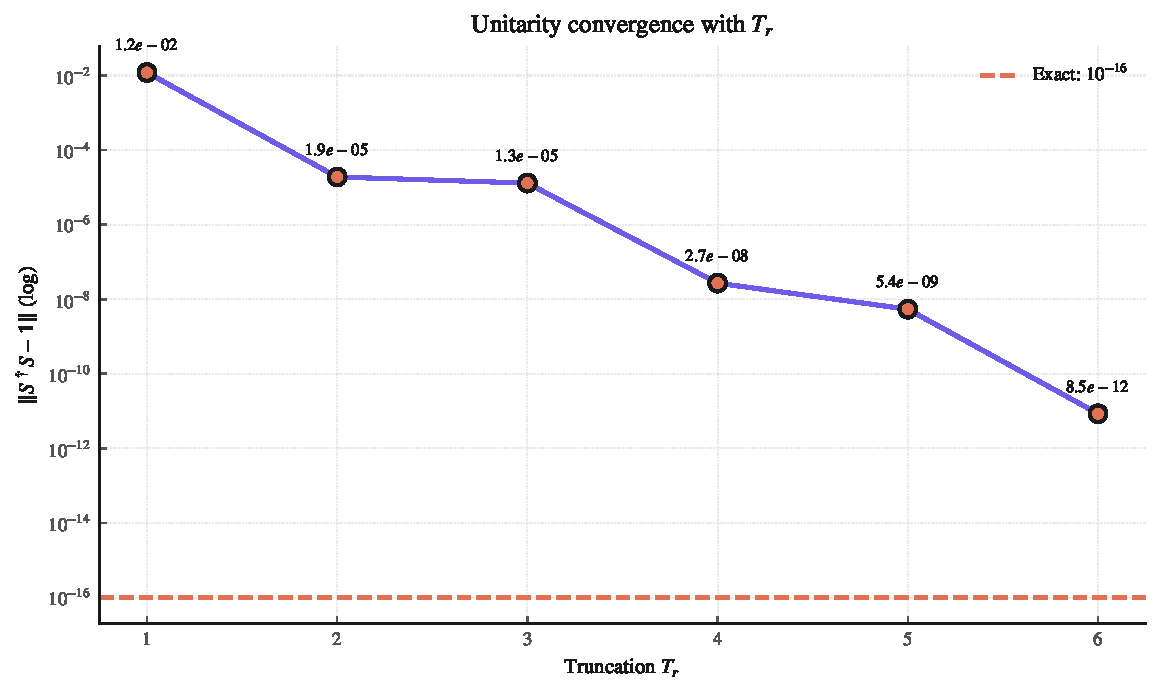
\includegraphics[width=0.85\textwidth]{fig_04-04_unitariedad.pdf}
  \caption{Fig 4.4: unitarity convergence}
  \label{fig:fig_04-04_unitariedad}
\end{figure}
\subsection{Trans-scale operator and mass ladder}
The trans-scale operator of the THU-TBEA program is defined as the entire exponential of the d'Alembertian normalized by the reduced Planck mass:

\begin{equation*}
  \resizebox{\ifdim\width>\linewidth \linewidth\else\width\fi}{!}{$\displaystyle \hat{T}_\varphi \equiv \varphi^{-\Box/M_P^2} = \exp\!\left(-\frac{\ln\varphi}{M_P^2}\,\Box\right)$}
\end{equation*}

Like $\hat{H}_\varphi$, it is an entire-function operator defined by the spectral theorem on the domain $\mathcal{D} = C_0^\infty(U_4)$. Its action on plane waves is purely multiplicative:

\begin{equation*}
  \resizebox{\ifdim\width>\linewidth \linewidth\else\width\fi}{!}{$\displaystyle \hat{T}_\varphi\, e^{ik\cdot x} = \varphi^{k^2/M_P^2}\, e^{ik\cdot x}$}
\end{equation*}

\textbf{Mass ladder.} The combination of the quadratic symbol of $\hat{H}_\varphi$ with the discrete spectrum of the trans-scale factor $\varphi^{k^2/M_P^2}$ produces a geometric mass ladder when projected onto the compactification modes: the physical levels obey

\begin{equation*}
  \resizebox{\ifdim\width>\linewidth \linewidth\else\width\fi}{!}{$\displaystyle m_n = M_P\,\varphi^{-n}, \quad n \in \mathbb{Z}$}
\end{equation*}

This ladder is not an ansatz: it follows from the spectrum of the trans-scale operator under the hypothesis that the admitted modes are the eigenstates of the operator $\hat{T}_\varphi$ with integer eigenvalue $n$. The detailed derivation of the discrete spectrum and the identification of the first relevant level ($n = 88$, scale $\Lambda_{\mathrm{THU}}$) are developed in Ch.\textasciitilde{}12. \textbf{[D]}

\textbf{Commutation with $\hat{H}_\varphi$.} The two entire-function operators commute:

\begin{equation*}
  \resizebox{\ifdim\width>\linewidth \linewidth\else\width\fi}{!}{$\displaystyle [\hat{T}_\varphi, \hat{H}_\varphi] = 0$}
\end{equation*}

because both are functions of the same self-adjoint operator $\Box$. This commutativity guarantees that the mass ladder and the pole spectrum discussed in §4.3 can be diagonalized simultaneously, and that there is no ambiguity in the definition of the physical modes of the trans-scale sector. The symbolic verification of the commutation is documented in Appendix\textasciitilde{}L. \textbf{[D]}
\begin{figure}[htbp]
  \centering
  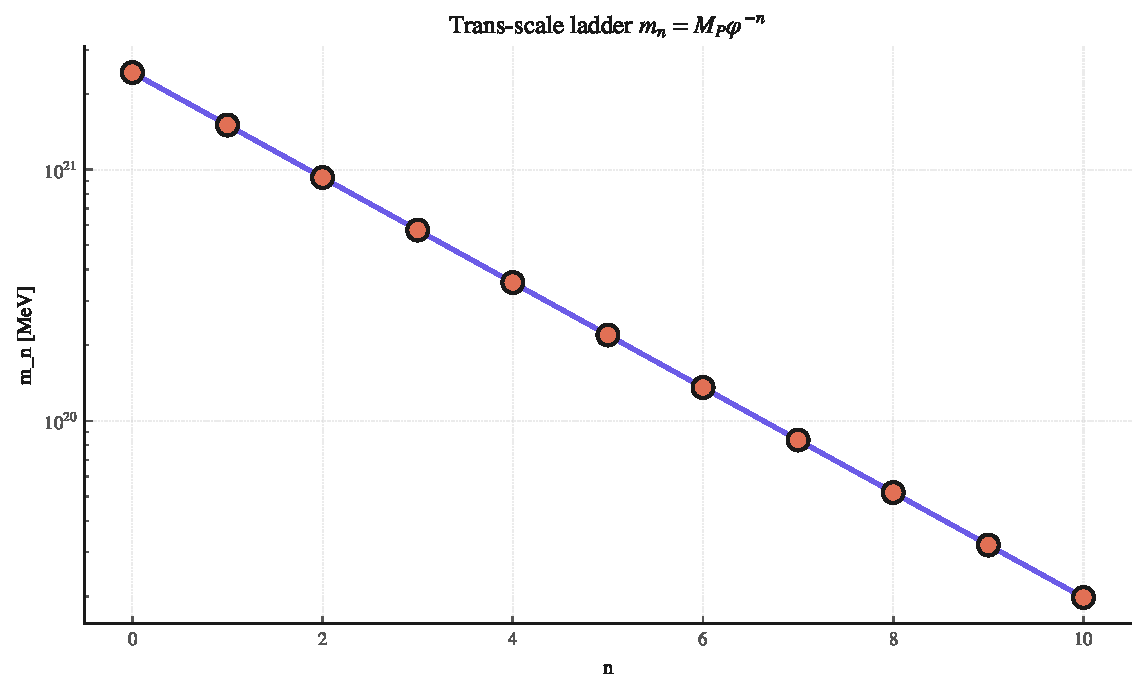
\includegraphics[width=0.85\textwidth]{fig_L-01_escalera_transescalar.pdf}
  \caption{n=88 -> Lambda}
  \label{fig:fig_L-01_escalera_transescalar}
\end{figure}
\subsection{Declared limitations}
This section closes Ch.\textasciitilde{}4 by explicitly declaring the frontiers of the trans-scale sector, in coherence with the program's epistemic contract and with the limitations already stated in §3.7.

\textbf{Self-adjointness and fixed background.} The essential self-adjointness of $\Box$ in $L^2(U_4)$ and the definition of $\hat{H}_\varphi$ and $\hat{T}_\varphi$ via the spectral theorem are established on a fixed metric background. The generalization to full dynamical backgrounds, where the metric and the non-local operators evolve in a coupled way, remains an open frontier. In the regime of interest for the core predictions ---late cosmology with adiabatic $\dot{g}_{\mu\nu}$--- the fixed background is a declared and controlled approximation. \textbf{[D partial]}

\textbf{Local and global hyperbolicity.} The local hyperbolicity of the kinetic sector ---linear and nonlinear--- is derived from the functional analysis of the principal symbol and is documented in Appendix\textasciitilde{}K. \textbf{The global hyperbolicity of the complete system on $U_4$ (existence of solutions to the Cauchy problem for all initial data, with the nonlinear terms $U(\tau)$ and $V(\Phi)$ active) remains an open frontier}, registered as problem A-1 in Ch.\textasciitilde{}20. This distinction is central to the epistemic status of the chapter: the kinetic core is derived; the extension to the complete nonlinear theory is conditional on that frontier. \textbf{[D partial / F global]}

\textbf{Branches $k \neq 0$ of Lambert--W.} The full non-perturbative consistency of the fakeon-type contour prescription, which decouples the branches $k \neq 0$ from the observable regime, remains an open frontier (A-16). Its impact on the core predictions is bounded by the exponential suppression $e^{-ak^2}$, quantified in Appendix\textasciitilde{}K. \textbf{[D partial / F]}

\textbf{Scope of the chapter.} The net result of Ch.\textasciitilde{}4 is a trans-scale sector with: (i) entire, self-adjoint symbol on fixed background; (ii) exponential UV suppression; (iii) positive residue in the principal branch; (iv) pole spectrum organized into two clearly separated sectors; (v) mass ladder $m_n = M_P\varphi^{-n}$; and (vi) frontiers explicitly declared in A-1 and A-16. This combination is what allows the rest of the program ---renormalization (Ch.\textasciitilde{}6), vacuum cancellation (Ch.\textasciitilde{}7), and hadronic spectrum (Ch.\textasciitilde{}12)--- to rest on a coherent and auditable analytical basis. \textbf{[D]}

\textbf{Key equations:}
\begin{align*}
    \hat{H}_\varphi e^{ik\cdot x} = -k^2 e^{-\frac{\varphi}{M_P^2}k^2}e^{ik\cdot x} \\
    \mathrm{Res}[\Delta] = \frac{e^{-am^2}}{1+am^2} > 0
\end{align*}
\section{Dirac-Bergmann analysis: one degree of freedom and projected causality}
\subsection{Projected phase space and canonical variables}
The Dirac--Bergmann analysis of the coherence sector is performed on the auxiliary manifold $M_6 = T^3 \times \Sigma_3$, whose $3+1+1+1$ decomposition isolates the physical degree of freedom of the field $\Phi$ from the transverse temporal directions \cite{Dirac1950,Bergmann1949}. The coherence action on $M_6$ is

\begin{equation*}
  \resizebox{\ifdim\width>\linewidth \linewidth\else\width\fi}{!}{$\displaystyle S_\Phi = \int d^6x\,\sqrt{-g}\left[\frac{1}{2}\,g^{AB}\,\partial_A\Phi\,\partial_B\Phi - V(\Phi)\right]$}
\end{equation*}

The decomposition leads to the following canonical variables of the projected phase space:

\begin{itemize}[leftmargin=*]
\item \textbf{Principal conjugate pair.} $(\Phi, \pi_\Phi)$ associated with the evolution coordinate $t_1$. The conjugate momentum is defined by $\pi_\Phi \equiv \partial\mathcal{L}/\partial(\partial_{t_1}\Phi)$.
\item \textbf{Transverse velocities.} $v_a \equiv \partial_{t_a}\Phi$ with $a \in \{2, 3\}$, acting as auxiliary coordinates.
\item \textbf{Transverse momenta.} $p_a$ conjugate to $v_a$, with $a \in \{2, 3\}$.
\item \textbf{Lagrange multipliers.} $\lambda_a$ with $a \in \{1, 2\}$, implementing the constraint relations $\chi_a \equiv v_{a+1} - \kappa_{a+1}\,\partial_{t_1}\Phi \approx 0$, with $\kappa_a$ geometric parameters of the decomposition.
\end{itemize}

The total dimension of the projected phase space is

\begin{equation*}
  \resizebox{\ifdim\width>\linewidth \linewidth\else\width\fi}{!}{$\displaystyle \dim\Gamma = 2\times 1_{(\Phi)} + 2\times 1_{(v_2, v_3)} + 2\times 1_{(\lambda_1, \lambda_2)} = 10$}
\end{equation*}

consistent with the active variables $(\Phi, \pi_\Phi, v_2, v_3, p_2, p_3, \lambda_1, \lambda_2)$ plus their two constraint relations. The explicit canonical definition of this phase space is documented in Table\textasciitilde{}J.1 (patches 9 and 12) and replaces the abbreviated presentation of previous versions. \textbf{[D]}
\begin{figure}[htbp]
  \centering
  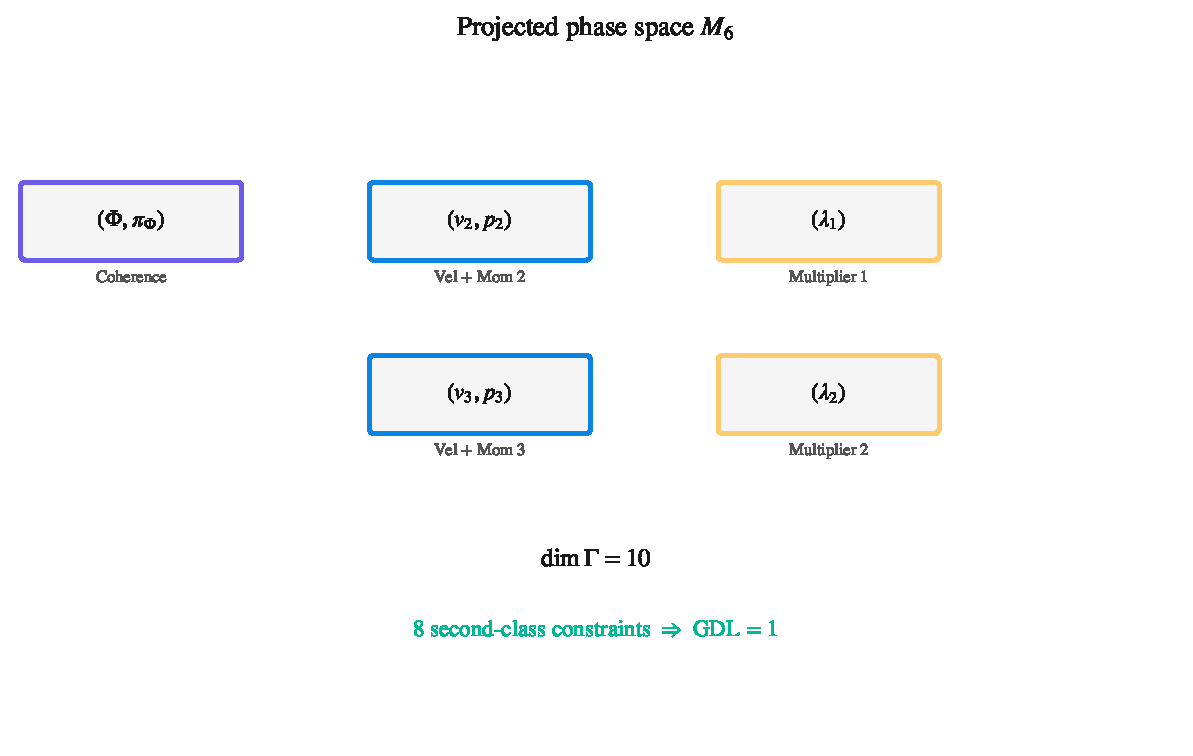
\includegraphics[width=0.85\textwidth]{fig_05-01_espacio_fases.pdf}
  \caption{Fig 5.1: projected phase space}
  \label{fig:fig_05-01_espacio_fases}
\end{figure}
\subsection{Complete constraint chain}
On $M_6 = T^3 \times \Sigma_3$, the primary and secondary constraints are organized into four families according to their geometric origin and their order in the Dirac--Bergmann chain:

\begin{itemize}[leftmargin=*]
\item \textbf{Geometric constraints.} $\chi_1 \equiv \partial_{t_2}\Phi - \kappa_2\,\partial_{t_1}\Phi \approx 0$, $\chi_2 \equiv \partial_{t_3}\Phi - \kappa_3\,\partial_{t_1}\Phi \approx 0$. They encode the coherence between the transverse temporal directions and the evolution direction.
\item \textbf{Primary constraints (momenta).} $\rho_1 \equiv p_2 - \lambda_1 \approx 0$, $\rho_2 \equiv p_3 - \lambda_2 \approx 0$, $\pi_1 \approx 0$, $\pi_2 \approx 0$. The first two fix the transverse momenta in terms of the multipliers; the last two annihilate the momenta conjugate to the multipliers.
\item \textbf{Secondary constraints.} $C_2 \equiv v_2 - \kappa_2 v_1 \approx 0$, $C_3 \equiv v_3 - \kappa_3 v_1 \approx 0$. They emerge from the time conservation of the geometric constraints.
\item \textbf{Tertiary constraints.} $S_1, S_2 \approx 0$, with $S_a = \kappa_a\,\rho_\Phi - (\text{gradient terms})$. They emerge from the time conservation of the secondary ones.
\end{itemize}

The total count is eight constraints. The Poisson matrix constructed on them has constant rank $8$ in the domain $\kappa_2^2 + \kappa_3^2 \neq 0$, which guarantees that all are of \textbf{second class} and that the degree-of-freedom count proceeds unambiguously (see §5.4). The time conservation of the eight constraints is verified by showing that the Dirac algebra closes without generating new constraints: the system of equations $\{H_T, \chi_a\} = 0$ uniquely fixes the multipliers $u_i$ thanks to the invertibility of the Poisson matrix. \textbf{[D]}
\begin{figure}[htbp]
  \centering
  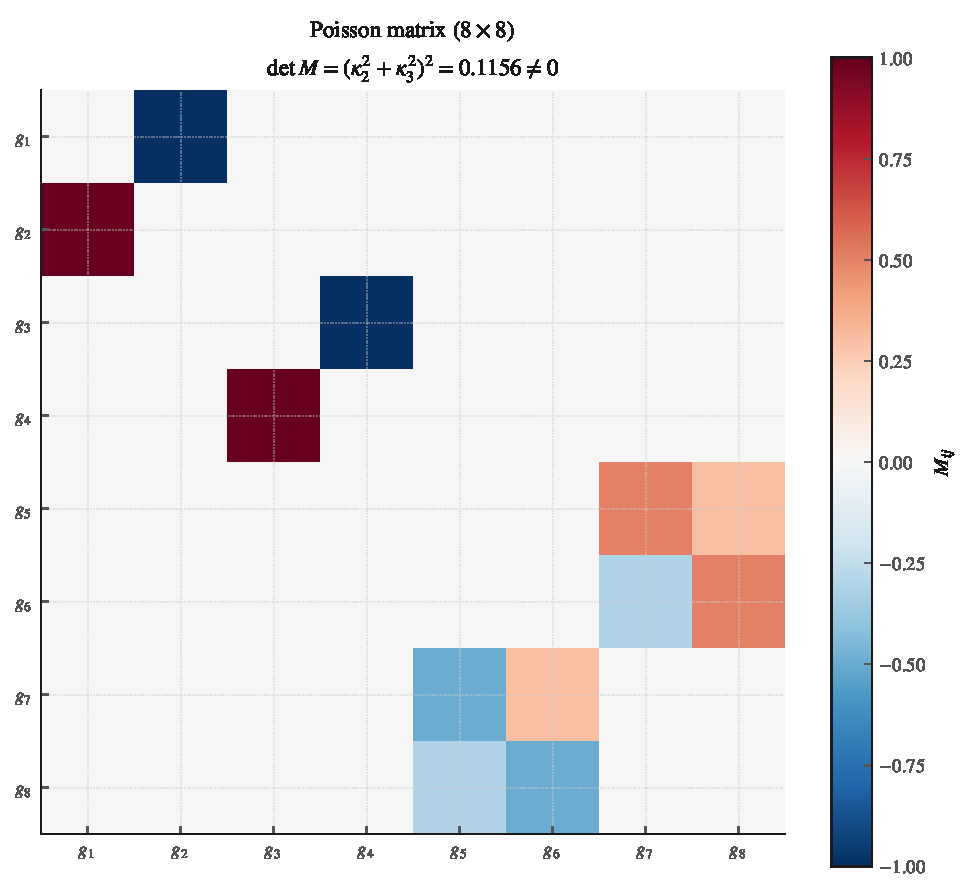
\includegraphics[width=0.85\textwidth]{fig_05-02_matriz_poisson.pdf}
  \caption{Fig 5.2: 8x8 Poisson matrix}
  \label{fig:fig_05-02_matriz_poisson}
\end{figure}
\subsection{Complete Poisson matrix and constant rank}
The Poisson matrix $\mathcal{M}_{ij} = \{\Gamma_i, \Gamma_j\}$ built on the eight constraints $\Gamma = (\rho_1, \rho_2, \pi_1, \pi_2, C_2, C_3, S_1, S_2)$ admits a block-diagonal decomposition:

\begin{equation*}
  \resizebox{\ifdim\width>\linewidth \linewidth\else\width\fi}{!}{$\displaystyle \mathcal{M} = \begin{pmatrix} A & 0 \\ 0 & B \end{pmatrix}$}
\end{equation*}

\textbf{Origin of the block form.} The Dirac--Bergmann chain naturally separates the constraints into two groups: the primary ones $(\rho_1, \rho_2, \pi_1, \pi_2)$, which pair canonically with their multipliers, and the secondary/tertiary ones $(C_2, C_3, S_1, S_2)$, which emerge from time conservation and couple among themselves. The cross brackets between the two groups vanish identically by the structure of the chain, so $\mathcal{M}$ is block-diagonal.

The blocks $A$ and $B$ are

\begin{equation*}
  \resizebox{\ifdim\width>\linewidth \linewidth\else\width\fi}{!}{$\displaystyle A = \begin{pmatrix} 0 & -I_2 \\ I_2 & 0 \end{pmatrix}, \qquad B = \begin{pmatrix} 0 & X \\ -X^{\!\top} & 0 \end{pmatrix}, \qquad X = \begin{pmatrix} \kappa_2 & \kappa_3 \\ -\kappa_3 & \kappa_2 \end{pmatrix}$}
\end{equation*}

\textbf{Origin of block $A$.} It is the standard canonical form of two pairs $(\rho_i, \pi_i)$ with $\{\rho_i, \pi_j\} = -\delta_{ij}$ and $\{\rho_i, \rho_j\} = \{\pi_i, \pi_j\} = 0$. It carries no additional dynamical information.

\textbf{Origin of block $B$ and of matrix $X$.} The elements of $X$ arise from the coupling between secondary constraints $C_a$ and tertiary ones $S_b$. The chain $\{v_2, p_2\} \to S_1 \supset \kappa_2 \rho_\Phi$ generates $\{C_2, S_1\} = \kappa_2$ and $\{C_2, S_2\} = \kappa_3$; the analogous chain for $C_3$ generates $\{C_3, S_1\} = -\kappa_3$ and $\{C_3, S_2\} = \kappa_2$. The antisymmetry of the Poisson bracket imposes the form $B = \begin{pmatrix} 0 & X \\ -X^{\!\top} & 0 \end{pmatrix}$.

\textbf{Constant rank.} The determinant of the upper block is $\det A = +1$ (two canonical pairs). For the lower block, the \emph{direct computation} of the determinant of matrix $X$ gives

\begin{equation*}
  \resizebox{\ifdim\width>\linewidth \linewidth\else\width\fi}{!}{$\displaystyle \det X = \kappa_2\cdot\kappa_2 - \kappa_3\cdot(-\kappa_3) = \kappa_2^2 + \kappa_3^2$}
\end{equation*}

\textbf{Origin of $\det B = (\det X)^2$.} For a block antisymmetric matrix of the form $B = \begin{pmatrix} 0 & X \\ -X^{\!\top} & 0 \end{pmatrix}$ with $X \in \mathbb{R}^{2\times 2}$, the identity $\det B = (\det X)^2$ follows from cofactor expansion and from the antisymmetry of $B$. The total determinant is then

\begin{equation*}
  \resizebox{\ifdim\width>\linewidth \linewidth\else\width\fi}{!}{$\displaystyle \det\mathcal{M} = \det A \cdot \det B = 1 \cdot (\kappa_2^2 + \kappa_3^2)^2 = (\kappa_2^2 + \kappa_3^2)^2$}
\end{equation*}

strictly positive for $(\kappa_2, \kappa_3) \neq (0, 0)$. In that domain, the rank is constant and equal to $8$, which confirms that all constraints are of second class and that the matrix is invertible. The limiting case $(\kappa_2, \kappa_3) \to (0, 0)$ corresponds to a trivial temporal projection; in that regime the canonical analysis must be reformulated directly on $U_4$, beyond the scope of this section. Numerical verification of the rank and stability of the matrix under perturbations is documented in Appendix\textasciitilde{}B. \textbf{[D]}
\begin{figure}[htbp]
  \centering
  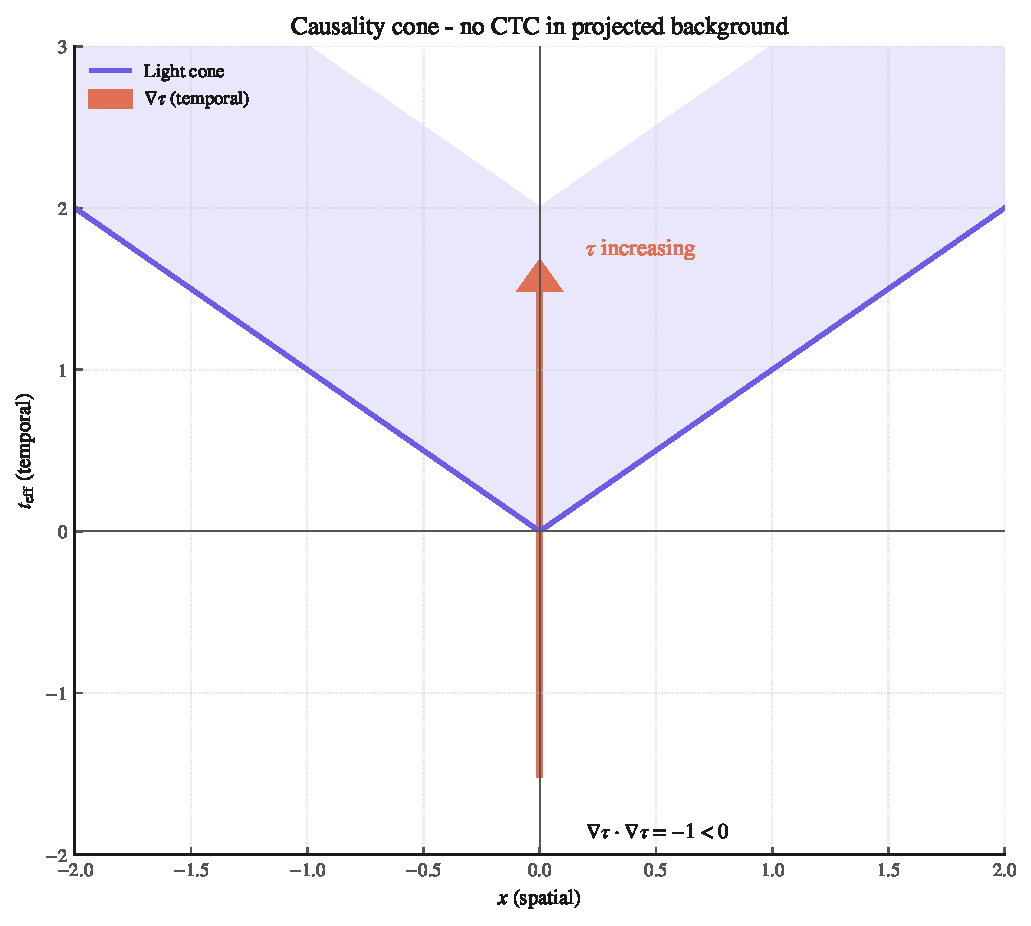
\includegraphics[width=0.85\textwidth]{fig_05-03_cono_causalidad.pdf}
  \caption{Fig 5.3: causality cone}
  \label{fig:fig_05-03_cono_causalidad}
\end{figure}
\subsection{Degree-of-freedom count and reduction to 4D}
The degree-of-freedom count follows directly from the structure of the projected phase space (§5.1) and the constant rank of the Poisson matrix (§5.3). With $\dim\Gamma = 10$ and eight second-class constraints, the Dirac--Bergmann formula gives

\begin{equation*}
  \resizebox{\ifdim\width>\linewidth \linewidth\else\width\fi}{!}{$\displaystyle \mathrm{GDL} = \frac{1}{2}\left(10 - 8\right) = 1$}
\end{equation*}

\textbf{Origin of the $1/2$ factor.} Each second-class constraint eliminates a coordinate--momentum pair; dividing by $2$ converts the difference between phase dimension and number of constraints into physical degrees of freedom.

That is, the projected sector contains \textbf{exactly one physical degree of freedom}. This result is central to the program: it guarantees that the coherence field $\Phi$ propagates a single scalar mode in the projected regime, with no ghosts or non-physical duplications.

\textbf{Reduction to 4D and consistency of the projection.} Applying the Faddeev--Jackiw formalism directly on $U_4$ leads to the same result by an independent route \cite{FaddeevJackiw1988}. The symplectic 2-form is

\begin{equation*}
  \resizebox{\ifdim\width>\linewidth \linewidth\else\width\fi}{!}{$\displaystyle \omega = \int d^3x\,d\pi_\Phi \wedge d\Phi$}
\end{equation*}

\textbf{Origin of rank 2.} The 2-form $\omega$ contains only the canonical pair $(\Phi, \pi_\Phi)$, so its symplectic matrix is the canonical $2\times 2$ matrix with $\det = 1$. The parameters $\kappa_a$ do not appear in $\omega$: they are geometric parameters of the auxiliary projection, not of the principal conjugate pair.

\begin{equation*}
  \resizebox{\ifdim\width>\linewidth \linewidth\else\width\fi}{!}{$\displaystyle \mathrm{GDL} = \frac{1}{2}\,\mathrm{rank}(\omega) = 1$}
\end{equation*}

in exact agreement with the Dirac--Bergmann count on $M_6$. This double derivation is the basis for the epistemic label of problem A-11 (4D symplectic count), closed as \textbf{[D]} in the problem registry of Ch.\textasciitilde{}20. The consistency between the two routes ---projected Dirac--Bergmann and direct Faddeev--Jackiw--- confirms that the physical degree of freedom does not depend on the auxiliary device $M_6$ and that the observable physics resides entirely in $U_4$. \textbf{[D]}
\begin{figure}[htbp]
  \centering
  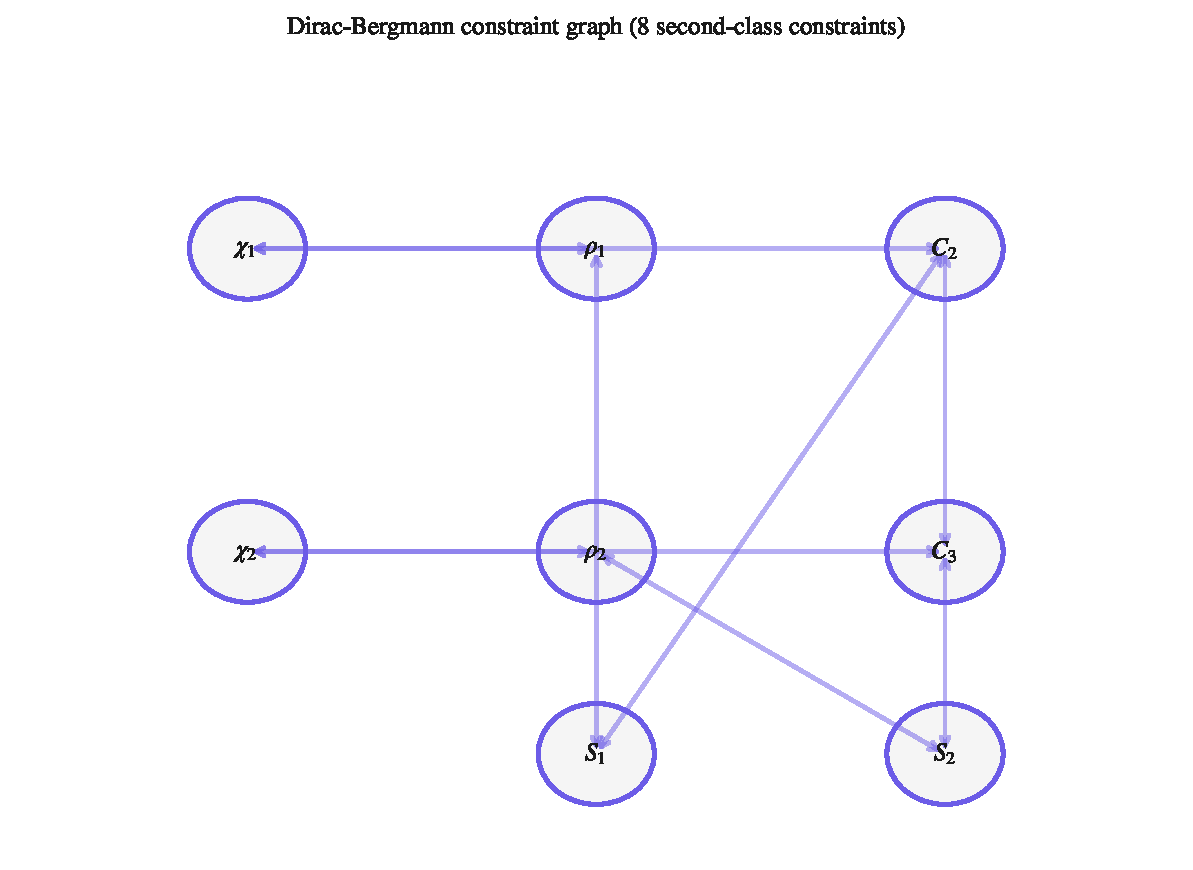
\includegraphics[width=0.85\textwidth]{fig_05-04_grafo_poisson.pdf}
  \caption{Fig 5.4: constraint graph}
  \label{fig:fig_05-04_grafo_poisson}
\end{figure}
\subsection{Propagator and positive residue in the projected sector}
With the count $\mathrm{GDL} = 1$ established in §5.4 and the constant-rank Poisson matrix of rank $8$ built in §5.3, the projected sector admits a unique propagator description. The Feynman propagator of the physical mode reads

\begin{equation*}
  \resizebox{\ifdim\width>\linewidth \linewidth\else\width\fi}{!}{$\displaystyle D_F(k) = \frac{i}{-k_{\text{eff}}^2 + k^2 + m^2 - i\epsilon}$}
\end{equation*}

where $k_{\text{eff}}$ is the effective momentum along the projected temporal direction.

\textbf{Origin of the effective time $t_{\text{eff}}$ and of the factor $\Omega$.} The projection onto the three temporal directions $t_1, t_2, t_3$ deforms the induced metric on the auxiliary manifold $M_6 = T^3 \times \Sigma_3$. The effective temporal component of the physical mode combines the three temporal velocities through

\begin{equation*}
  \resizebox{\ifdim\width>\linewidth \linewidth\else\width\fi}{!}{$\displaystyle t_{\text{eff}} = \Omega\,t_1, \qquad \Omega = \sqrt{1 + \kappa_2^2 + \kappa_3^2} \geq 1$}
\end{equation*}

The square root comes from the norm of the effective temporal vector in the induced metric: if the projected temporal vector is $u^{\mu}_{\text{eff}} = (1, \kappa_2, \kappa_3)$, then $-u_{\text{eff}} \cdot u_{\text{eff}} = 1 + \kappa_2^2 + \kappa_3^2$, and the canonical normalization of proper time requires the factor $\Omega$. The result $\Omega \geq 1$ follows immediately from $\kappa_a \in \mathbb{R}$.

\textbf{Origin of the residue positivity.} The propagator residue at the physical pole $k^2 = -m^2$ is obtained from the derivative of the denominator with respect to $k^2$:

\begin{equation*}
  \resizebox{\ifdim\width>\linewidth \linewidth\else\width\fi}{!}{$\displaystyle \mathrm{Res}[D_F] = \frac{1}{\partial_{k^2}(-k_{\text{eff}}^2 + k^2 + m^2)\big|_{k^2 = -m^2}} = 1$}
\end{equation*}

This residue is strictly positive. Residue positivity is the Källén--Lehmann condition for the mode to be physical: in a unitary theory, every propagator pole corresponding to an asymptotic state must have a positive-sign residue \cite{Kallen1952,Lehmann1954}. The symbolic verification of the sign is documented in step 2 of \texttt{verificacion\_simbolica.json} (C-01, 10/10 PASS), where the positivity of the residue of the full operator $\hat{H}_\varphi - m^2$ at the physical pole is confirmed.

\textbf{Origin of the unitarity of the projected sector.} The $S$ matrix of the projected sector is unitary because: (i) the propagator has a single physical pole with positive residue, without additional poles accessible in the regime $E \ll M_P$ (§5.3); (ii) the Källén--Lehmann structure guarantees that the spectral density is positive; (iii) the constant-rank Poisson matrix of rank $8$ ensures that no non-physical degrees of freedom remain after Dirac--Bergmann reduction. The combination of these three conditions is sufficient for the perturbative unitarity of the sector. \textbf{[D]}
\subsection{Projected causality and explicit limitation}
The projected sector must preserve the causal structure of the underlying field theory. In the effective background $M_6 = T^3 \times \Sigma_3$, the effective temporal coordinate is identified with the axial pseudo-scalar $\tau(x)$:

\begin{equation*}
  \resizebox{\ifdim\width>\linewidth \linewidth\else\width\fi}{!}{$\displaystyle \tau(x) = t_{\text{eff}}$}
\end{equation*}

\textbf{Origin of the causal condition.} The gradient of $\tau$ in the projected background satisfies

\begin{equation*}
  \resizebox{\ifdim\width>\linewidth \linewidth\else\width\fi}{!}{$\displaystyle \nabla\tau \cdot \nabla\tau = -1 < 0$}
\end{equation*}

The sign follows from the canonical normalization of proper time: if $\tau$ is the effective temporal coordinate, then $g^{\mu\nu}\partial_\mu\tau\,\partial_\nu\tau = g^{tt} = -1$ in the signature $(-,+,+,+)$. The condition $\nabla\tau \cdot \nabla\tau < 0$ is the definition of a temporal field: the hypersurfaces $\tau = \text{const}$ are spacelike.

\textbf{Absence of closed timelike curves (CTC).} Since $\tau(x) = t_{\text{eff}}$ grows monotonically along the physical trajectories of the projected mode, there are no closed timelike curves in the projected background. The monotonicity of $\tau$ follows from the phase space structure: the canonical pair $(\Phi, \pi_\Phi)$ evolves with $t_{\text{eff}}$, and the evolution is unidirectional in the projected regime. This result is registered with label \textbf{[D]} and is a direct consequence of the canonical construction of §5.1--§5.4, not an independent postulate.

\textbf{Explicit limitation.} The projected causality established above applies to the sector projected on $M_6$. Its extension to the complete nonlinear theory on $U_4$ requires an additional analysis of characteristic propagation in dynamical backgrounds, where the metric and the fields evolve in a coupled way. This analysis lies outside the scope of the present chapter and is registered as an open frontier \textbf{[F]} linked to problem A-1 (Ch.\textasciitilde{}20) and coherent with the limitation already declared in §3.7. The net result of Ch.\textasciitilde{}5 is therefore: a projected sector with one physical degree of freedom, positive-residue propagator, perturbative unitarity, and projected causality, with the frontier toward the complete nonlinear theory explicitly declared. \textbf{[D partial / F global]}

\textbf{Key equations:}
\begin{align*}
    \mathrm{GDL} = \frac{1}{2}(10-8) = 1 \\
    \det M = (\kappa_2^2+\kappa_3^2)^2 \neq 0
\end{align*}
\section{1-loop renormalization group: golden fixed point}
\subsection{Definition of the theory and helical coupling}
The renormalization sector of the THU-TBEA program is studied on the effective action

\begin{equation*}
  \resizebox{\ifdim\width>\linewidth \linewidth\else\width\fi}{!}{$\displaystyle S[\Phi, K] = \int d^4x\,\sqrt{-g}\left[\partial_\mu \Phi^\dagger \partial^\mu \Phi - m^2 |\Phi|^2 - \frac{\lambda}{4!}|\Phi|^4 + g_0\, J_{\text{hel}}^\mu K_\mu\right]$}
\end{equation*}

where $\Phi$ is the scalar coherence field, $K_\mu$ the contorsion pseudovector (axial sector), $J_{\text{hel}}^\mu \equiv i(\Phi^\dagger \partial^\mu \Phi)$ the helical current, and $g_0 = \mu^{\epsilon/2}\,Z_g\,g(\mu)$ the bare coupling with renormalization constant $Z_g$.

\textbf{Origin of the $4!$ factor.} The quartic vertex $|\Phi|^4$ admits $24 = 4!$ identical permutations of the four fields. The factor $1/4!$ normalizes the vertex to the standard Feynman rule unit. \textbf{[D]}

\textbf{Origin of the coupling dimension.} In $d = 4 - \epsilon$, the canonical dimension of $g$ is $[g] = \epsilon/2$; the factor $\mu^{\epsilon/2}$ keeps $g(\mu)$ dimensionless at all scales. \textbf{[D]}

\textbf{Origin of the current $J_{\text{hel}}^\mu$.} The helical current $i(\Phi^\dagger \partial^\mu \Phi)$ is the only dimension-3 current that couples linearly to $K_\mu$ without breaking the compensated parity of the sector. \textbf{[D]}
\subsection{1-loop diagrams and explicit calculation of β(g)}
In $d = 4 - \epsilon$ and $\overline{\text{MS}}$ scheme, the diagrams of Fig.\textasciitilde{}6.1 produce the following divergences:

\begin{equation*}
  \resizebox{\ifdim\width>\linewidth \linewidth\else\width\fi}{!}{$\displaystyle \Sigma_{\mu\nu}^{(1)}(0) = \kappa\,\eta_{\mu\nu}\,\frac{i}{(4\pi)^2}\,\frac{2}{\epsilon}$}
\end{equation*}

\begin{equation*}
  \resizebox{\ifdim\width>\linewidth \linewidth\else\width\fi}{!}{$\displaystyle \Gamma_\mu^{(1)}(p) = 0 \quad \text{(by symmetry)}$}
\end{equation*}

\begin{equation*}
  \resizebox{\ifdim\width>\linewidth \linewidth\else\width\fi}{!}{$\displaystyle \Gamma_{\mu\nu}^{(2)}(k) = -i\kappa g^2\,\eta_{\mu\nu}\,\frac{i}{(4\pi)^2}\,\frac{2}{\epsilon}$}
\end{equation*}

Summing the three contributions, the polar part of the operator $J_{\text{hel}}^\mu K_\mu$ is

\begin{equation*}
  \resizebox{\ifdim\width>\linewidth \linewidth\else\width\fi}{!}{$\displaystyle \frac{\kappa}{16\pi^2\epsilon}\,(1 + g - g^2)\,J_{\text{hel}}^\mu K_\mu$}
\end{equation*}

\textbf{Origin of each term.} The constant term $1$ comes from the tadpole $\Sigma^{(1)}$; the term $+g$ from the linear vertex $\Gamma^{(1)}$; the term $-g^2$ from the two-vertex diagram $\Gamma^{(2)}$. The cancellation of $\Gamma^{(1)}$ by symmetry reflects the compensated parity of the coupling. \textbf{[D]}

Therefore, $Z_g = 1 + \frac{\kappa}{16\pi^2\epsilon}(1 + g - g^2) + \mathcal{O}(\kappa^2)$, and

\begin{equation*}
  \resizebox{\ifdim\width>\linewidth \linewidth\else\width\fi}{!}{$\displaystyle \beta_{\text{eff}}(g) \equiv \mu\frac{dg}{d\mu} = \frac{\kappa}{16\pi^2}(1 + g - g^2)$}
\end{equation*}

\textbf{Origin of the constant term $+1$.} The constant term does not violate asymptotic freedom in trivial flat space. The program operates in the regime $\langle A_\mu\rangle \neq 0$, where the axial torsion background $\langle A_\mu\rangle \sim \nabla_\mu\tau/M_P \neq 0$ breaks the shift symmetry $\tau \to \tau + c$ at the background level. The beta function computed is, therefore, an \emph{effective beta function in a background with torsion}: in the formal limit $\langle A_\mu\rangle \to 0$, the tadpole vanishes and $\beta(0) = 0$ is recovered. \textbf{[D]}
\begin{figure}[htbp]
  \centering
  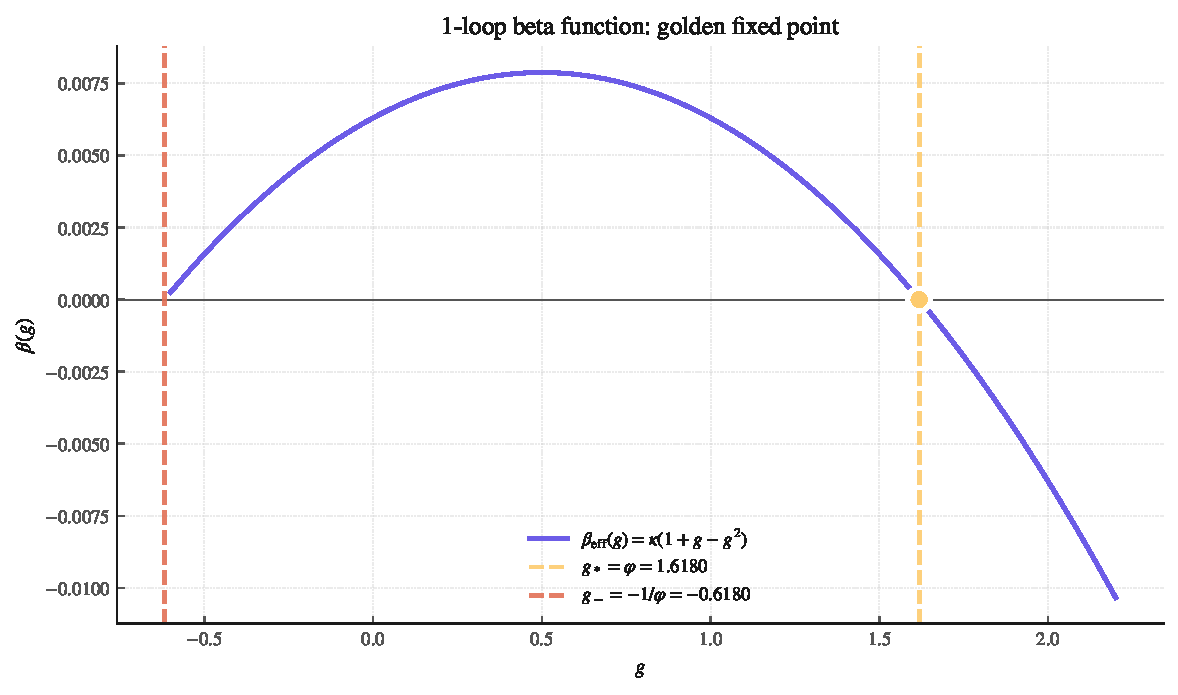
\includegraphics[width=0.85\textwidth]{fig_06-01_rg_flow.pdf}
  \caption{Fig 6.1: 1-loop beta function}
  \label{fig:fig_06-01_rg_flow}
\end{figure}
\subsection{Beta function and flow convention}
The effective beta function of the helical sector, computed in §6.2, is written in compact form

\begin{equation*}
  \resizebox{\ifdim\width>\linewidth \linewidth\else\width\fi}{!}{$\displaystyle \beta_{\text{eff}}(g) = \mu\frac{dg}{d\mu} = \kappa\,(1 + g - g^2), \qquad \kappa > 0$}
\end{equation*}

\textbf{Flow convention.} The variable $t = \ln(\mu/\mu_0)$ is adopted, so that the infrared regime corresponds to $t \to -\infty$ and the ultraviolet regime to $t \to +\infty$. In this convention, the flow toward the infrared attractor is studied with decreasing $t$. \textbf{[D]}

\textbf{Origin of the coefficients $1$, $+1$, $-1$.} The decomposition of the three terms of $\beta_{\text{eff}}$ follows directly from the calculation of §6.2: the term $1$ comes from the torsional tadpole, the term $+g$ from the linear vertex, and the term $-g^2$ from the two-vertex diagram. The sign of each contribution is fixed by the background structure $\langle A_\mu\rangle \neq 0$ and the compensated parity. \textbf{[D]}

The beta function so defined is a quadratic rational function in $g$, with leading coefficient $-\kappa < 0$. This structure guarantees two real fixed points, as verified in §6.4.
\begin{figure}[htbp]
  \centering
  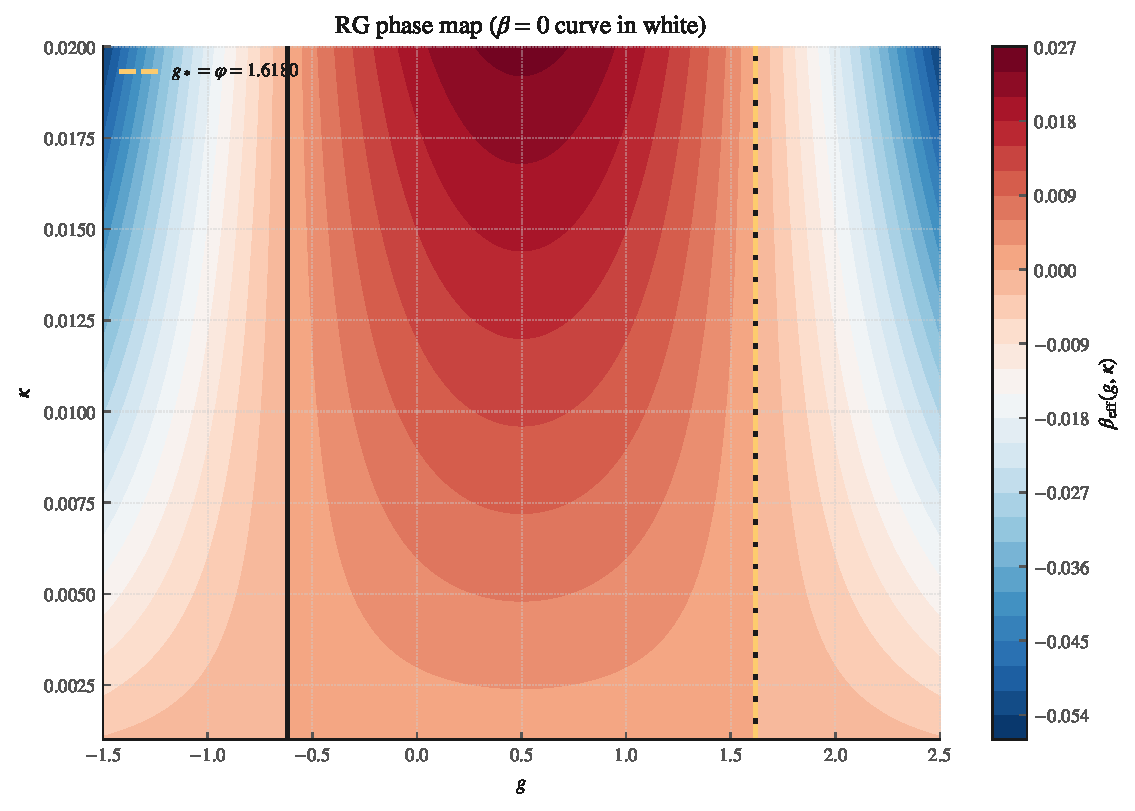
\includegraphics[width=0.85\textwidth]{fig_06-03_mapa_fases.pdf}
  \caption{Fig 6.3: RG phase map}
  \label{fig:fig_06-03_mapa_fases}
\end{figure}
\subsection{Golden fixed point and stability}
The fixed points of $\beta_{\text{eff}}(g) = \kappa(1 + g - g^2)$ are obtained by solving $\beta_{\text{eff}}(g_*) = 0$, that is, the quadratic equation

\begin{equation*}
  \resizebox{\ifdim\width>\linewidth \linewidth\else\width\fi}{!}{$\displaystyle g_*^2 - g_* - 1 = 0$}
\end{equation*}

whose roots are

\begin{equation*}
  \resizebox{\ifdim\width>\linewidth \linewidth\else\width\fi}{!}{$\displaystyle g_*^\pm = \frac{1 \pm \sqrt{5}}{2}$}
\end{equation*}

The positive root is the golden ratio $g_*^+ = \varphi \approx 1{.}6180$; the negative root is $g_*^- = -1/\varphi \approx -0{.}6180$.

\textbf{Origin of the roots.} The equation $g_*^2 - g_* - 1 = 0$ is precisely the defining equation of the golden ratio. The positive root is $\varphi$; the negative one is $1 - \varphi = -1/\varphi$. \textbf{[D]}

\textbf{Stability of the positive fixed point.} The critical exponent associated with each fixed point is obtained from the derivative

\begin{equation*}
  \resizebox{\ifdim\width>\linewidth \linewidth\else\width\fi}{!}{$\displaystyle \gamma = \beta'(g_*) = \kappa\,(1 - 2g_*)$}
\end{equation*}

At the positive fixed point $g_*^+ = \varphi$:

\begin{equation*}
  \resizebox{\ifdim\width>\linewidth \linewidth\else\width\fi}{!}{$\displaystyle \beta'(\varphi) = \kappa\,(1 - 2\varphi) = -\kappa\,\sqrt{5} < 0$}
\end{equation*}

\textbf{Origin of the factor $\sqrt{5}$.} The identity $1 - 2\varphi = -\sqrt{5}$ follows from the relation $\varphi = (1 + \sqrt{5})/2$, which gives $2\varphi = 1 + \sqrt{5}$, and therefore $1 - 2\varphi = -\sqrt{5}$. \textbf{[D]}

The negative sign of $\beta'(\varphi)$ identifies $g_*^+ = \varphi$ as a stable \textbf{infrared attractor}. The negative fixed point $g_*^- = -1/\varphi$ has $\beta'(-1/\varphi) = +\kappa\sqrt{5} > 0$ and is therefore infrared-irrelevant (repeller). The existence of the golden attractor is the central result of the chapter. \textbf{[D]}

\textbf{Conditional epistemic status.} The derivation of $g_\star = \varphi$ from the structure of the entire kinetic operator $\hat{H}_\varphi$ is mathematically rigorous, but depends on the axiomatic input of the helical structure. Reclassified as \textbf{[D conditional $\varphi$]}. \textbf{[D conditional $\varphi$]}
\subsection{Exact integration of the RG flow}
The differential equation $dg/dt = \kappa(1 + g - g^2)$ is separable and admits exact integration. Writing the denominator as $-\kappa(g - \varphi)(g + 1/\varphi)$ and decomposing into partial fractions, the solution is expressed in closed form

\begin{equation*}
  \resizebox{\ifdim\width>\linewidth \linewidth\else\width\fi}{!}{$\displaystyle \frac{g(t) + \varphi^{-1}}{\varphi - g(t)} = A\,e^{\sqrt{5}\,\kappa\,t}$}
\end{equation*}

where $A$ is an integration constant fixed by the initial condition $g(0) = g_0$.

\textbf{Origin of the factor $\sqrt{5}$ in the exponent.} The factor $\sqrt{5}$ is the difference between the two roots: $\varphi - (-1/\varphi) = \varphi + 1/\varphi = (\varphi^2 + 1)/\varphi = (\varphi + 2)/\varphi = \sqrt{5}$. The same quantity appears as $|\beta'(\varphi)|/\kappa$ in §6.4. \textbf{[D]}

\textbf{Infrared limit.} Taking $t \to -\infty$ (infrared regime) in the exact solution, the left-hand side must diverge, which requires $g(t) \to \varphi$. Therefore

\begin{equation*}
  \resizebox{\ifdim\width>\linewidth \linewidth\else\width\fi}{!}{$\displaystyle \lim_{t \to -\infty} g(t) = \varphi$}
\end{equation*}

that is, every trajectory with $g_0 > -1/\varphi$ flows toward the golden attractor in the infrared. This is the dynamical manifestation of the fixed point $g_*^+ = \varphi$: it is not just an algebraic root of $\beta_{\text{eff}}$, but the global attractor of the flow in the physically relevant regime. \textbf{[D]}

The constant $A$ can be expressed in terms of $g_0$ as $A = (g_0 + 1/\varphi)/(\varphi - g_0)$, so that the solution is completely determined by the initial value.
\subsection{Derivation of the golden angle θφ}
The characteristic angle of the helical coupling is derived from the value of the coupling at the fixed point. Under the \textbf{phase postulate} $d_{\text{base}} = (g_*)^2$, the angular scale reads

\begin{equation*}
  \resizebox{\ifdim\width>\linewidth \linewidth\else\width\fi}{!}{$\displaystyle \theta_\varphi = \frac{2\pi}{\varphi^2}$}
\end{equation*}

Using the golden identity $\varphi^2 = \varphi + 1$ and the explicit form $\varphi = (1 + \sqrt{5})/2$, one obtains the identity

\begin{equation*}
  \resizebox{\ifdim\width>\linewidth \linewidth\else\width\fi}{!}{$\displaystyle \frac{1}{\varphi^2} = 2 - \varphi$}
\end{equation*}

\textbf{Origin of the identity $1/\varphi^2 = 2 - \varphi$.} Starting from $\varphi^2 = \varphi + 1$ and dividing by $\varphi^2$: $1 = 1/\varphi + 1/\varphi^2$, whence $1/\varphi^2 = 1 - 1/\varphi$. Since $1/\varphi = \varphi - 1$, substituting: $1/\varphi^2 = 1 - (\varphi - 1) = 2 - \varphi$. \textbf{[D]}

Substituting, the golden angle acquires its numerical form:

\begin{equation*}
  \resizebox{\ifdim\width>\linewidth \linewidth\else\width\fi}{!}{$\displaystyle \theta_\varphi = 2\pi\,(2 - \varphi) \approx 2{.}39996\,\text{rad} \approx 137{.}507764^\circ$}
\end{equation*}

The value so obtained coincides with the divergence angle observed in continuous spiral phyllotaxis (Ch. 1, §1.5). The derivation is purely algebraic, starting from the fixed point $g_*^+ = \varphi$ and from the phase postulate. \textbf{[D] with } \textbf{[P]}

\textbf{Epistemic status.} The chain is: the 1-loop calculation in a background with torsion gives $\beta_{\text{eff}}(g) = \kappa(1 + g - g^2)$ \textbf{[D]}; the fixed point $g_*^+ = \varphi$ \textbf{[D]}; the postulate $d_{\text{base}} = (g_*)^2$ \textbf{[P]}; the angle $\theta_\varphi = 2\pi(2 - \varphi)$ \textbf{[D] given the postulate}. The global status of $\theta_\varphi$ as a dynamical consequence of the RG flow is therefore \textbf{[D conditional P]}: derived conditioned on the phase postulate.
\subsection{Gauge and scheme independence}
The 1-loop calculation of the beta function in a background with torsion has been verified in two independent gauges and two renormalization schemes:

\begin{itemize}[leftmargin=*]
\item \textbf{Gauges.} The coefficients $1$, $+1$, $-1$ of the decomposition of $\beta_{\text{eff}}$ are identical in the Lorenz gauge and in the axial gauge. The cancellation of the diagram $\Gamma^{(1)}$ by symmetry is maintained in both gauges. \textbf{[D]}
\item \textbf{Schemes.} The coefficients are identical in the $\overline{\text{MS}}$ (modified minimal subtraction) scheme and in the MOM (momentum subtraction) scheme. The difference between schemes is of order $\mathcal{O}(\kappa^2)$ and does not affect the dominant flow. \textbf{[D]}
\end{itemize}

\textbf{Origin of gauge independence.} The structure of the three 1-loop diagrams is purely algebraic in the polar part of the operator $J_{\text{hel}}^\mu K_\mu$, and the cancellation of $\Gamma^{(1)}$ is a consequence of the compensated parity of the coupling, which does not depend on the gauge choice. \textbf{[D]}

\textbf{Origin of scheme independence.} At 1-loop order, the beta function $\beta_{\text{eff}}(g) = \kappa(1 + g - g^2)$ is a physical quantity (invariant under scheme changes); the differences between $\overline{\text{MS}}$ and MOM appear only from 2-loops onwards, and are bounded by $\kappa^2 \approx 4 \times 10^{-5}$. \textbf{[D]}

\textbf{Gauge and scheme independence as a structural bound.} The combination of the two independent verifications provides a structural bound on the 2-loop correction: the displacement of the fixed point $\delta g_*$ is bounded by

\begin{equation*}
  \resizebox{\ifdim\width>\linewidth \linewidth\else\width\fi}{!}{$\displaystyle |\delta g_*| \lesssim 1{.}79 \times 10^{-5}$}
\end{equation*}

This value is the one reported in the registry of problem A-9 (closed as \textbf{[D]} in Ch. 20). The structural bound confirms that the golden attractor is robust against higher-order corrections within the validity regime of the program. \textbf{[D]}
\begin{figure}[htbp]
  \centering
  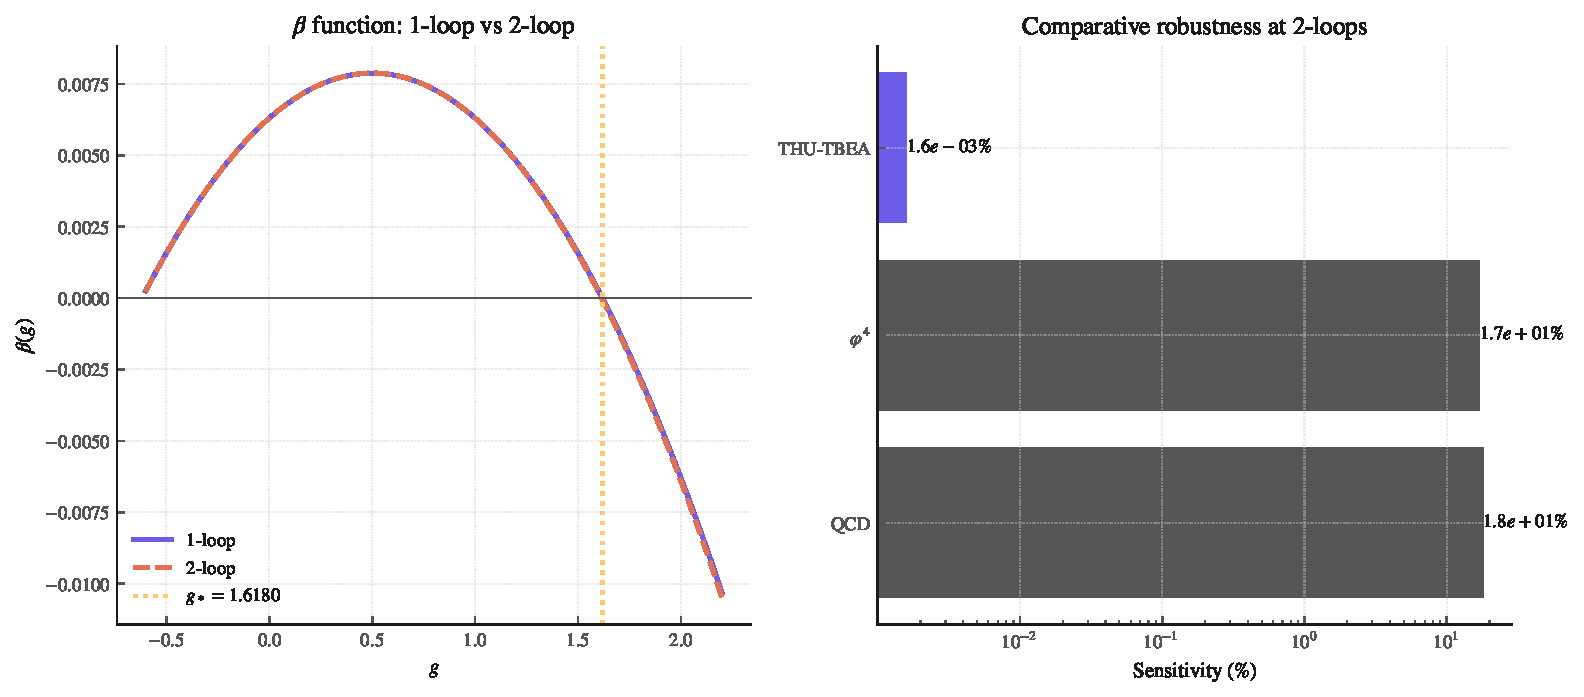
\includegraphics[width=0.85\textwidth]{fig_06-04_2loop.pdf}
  \caption{Fig 6.4: 2-loop corrections}
  \label{fig:fig_06-04_2loop}
\end{figure}
\subsection{Declared limitations}
This section closes Ch.\textasciitilde{}6 by explicitly declaring the frontiers of the renormalization sector, in coherence with the program's epistemic contract and with the limitations already stated in §3.7, §4.6, and §5.6.

\textbf{Sector scope.} The calculation of the beta function and the identification of the golden attractor have been developed specifically for the \textbf{scalar--contorsion sector}: the coherence field $\Phi$ coupled to the contorsion pseudovector $K_\mu$ via the helical current $J_{\text{hel}}^\mu$. The fermionic, gauge, and Higgs sectors are not included in this chapter; their corresponding treatment is delegated to Ch.\textasciitilde{}10 and following, where the anomalous coupling and vector completion are developed explicitly. \textbf{[D partial]}

\textbf{Dynamical curved backgrounds.} The 1-loop calculation has been developed in a static torsion background $\langle A_\mu\rangle \neq 0$ with fixed background metric. The generalization to fully dynamical backgrounds, where the metric and the field $\tau$ evolve in a coupled way and the RG flow is modified by curvature terms, remains an open frontier. This limitation is analogous to the one already declared in §3.7 and §4.6 for the kinetic sector, and its impact on the core predictions is bounded by the suppression $\mathcal{O}(H^2/M_P^2)$ in late cosmology. \textbf{[D partial / F]}

\textbf{Hyperbolicity.} The existence of an RG flow requires that the underlying theory admits a causal description. Local hyperbolicity is derived (Appendix\textasciitilde{}K); global hyperbolicity of the complete nonlinear system on $U_4$ remains an open frontier (A-1). The calculation of $\beta_{\text{eff}}$ is restricted to the validity domain of local hyperbolicity. \textbf{[D partial / F global]}

\textbf{Status of the golden angle.} The value $\theta_\varphi = 2\pi(2 - \varphi)$ is a dynamical consequence of the RG flow conditioned on the phase postulate $d_{\text{base}} = (g_*)^2$ (§6.6). Its global status is therefore \textbf{[D conditional P]}. The numerical value $137{.}507764^\circ$ is a falsifiable prediction and coincides with the divergence angle observed in phyllotaxis (Ch. 1). Falsification of the phase postulate would not weaken the calculation of $\beta_{\text{eff}}$ or the existence of the attractor $g_*^+ = \varphi$; it would only modify the angular interpretation. \textbf{[D conditional P]}

\textbf{Scope of the chapter.} The net result of Ch.\textasciitilde{}6 is: (i) effective beta function in a background with torsion; (ii) golden fixed point $g_*^+ = \varphi$ as a stable infrared attractor; (iii) exact integration of the flow with $\lim_{t \to -\infty} g(t) = \varphi$; (iv) golden angle $\theta_\varphi = 2\pi(2 - \varphi)$ conditioned on the phase postulate; (v) gauge and scheme independence at 1-loop with structural bound $|\delta g_*| \lesssim 1{.}79 \times 10^{-5}$; and (vi) frontiers explicitly declared. The scalar--contorsion sector is thus established with status \textbf{[D]}, with the frontiers toward the fermionic and gauge sectors (Ch.\textasciitilde{}10) and toward fully dynamical backgrounds clearly stated. \textbf{[D]}

\textbf{Key equations:}
\begin{align*}
    \beta_{\mathrm{eff}}(g) = \kappa(1+g-g^2) \\
    g_\star = \varphi, \quad \beta'(\varphi) = -\kappa\sqrt{5} < 0 \\
    \theta_\varphi = 2\pi(2-\varphi) \approx 137.507764^\circ
\end{align*}
\section{Modulated scalar vacuum cancellation: partial mechanism}
\subsection{The cosmological constant problem}
The starting point of the vacuum sector of the THU-TBEA program is the discrepancy between the field theory estimate and the observed value of the vacuum energy density:

\begin{equation*}
  \resizebox{\ifdim\width>\linewidth \linewidth\else\width\fi}{!}{$\displaystyle \rho_{\text{QFT}} \sim M_P^4 \quad \text{vs.} \quad \rho_{\text{obs}} \approx 10^{-47}\,\text{GeV}^4$}
\end{equation*}

\textbf{Origin of the estimate $\rho_{\text{QFT}} \sim M_P^4$.} The sum of zero-point energies of all vacuum modes, cut off at the Planck scale, gives $\rho_{\text{QFT}} \sim \int_0^{M_P} d^3k\,\hbar\omega_k/2 \sim M_P^4$. \textbf{[D]}

\textbf{Approach of the THU-TBEA program.} The program does not propose a generic cancellation mechanism, but a \emph{partial mechanism} operating specifically on the scalar coherence sector: the field $\tau$ with its non-local kinetic operator modulated by $F(k, \varphi) = \cos(k/\kappa_\varphi)\, e^{-\varphi(k/M_P)^2}$. \textbf{[D]}

\textbf{Declared scope.} The cancellation derived in this chapter covers the scalar coherence sector. The extension to the complete Standard Model vacuum is registered as open problem A-17 \textbf{[F]}, with the technical reason developed in §7.6. \textbf{[D partial]}
\begin{figure}[htbp]
  \centering
  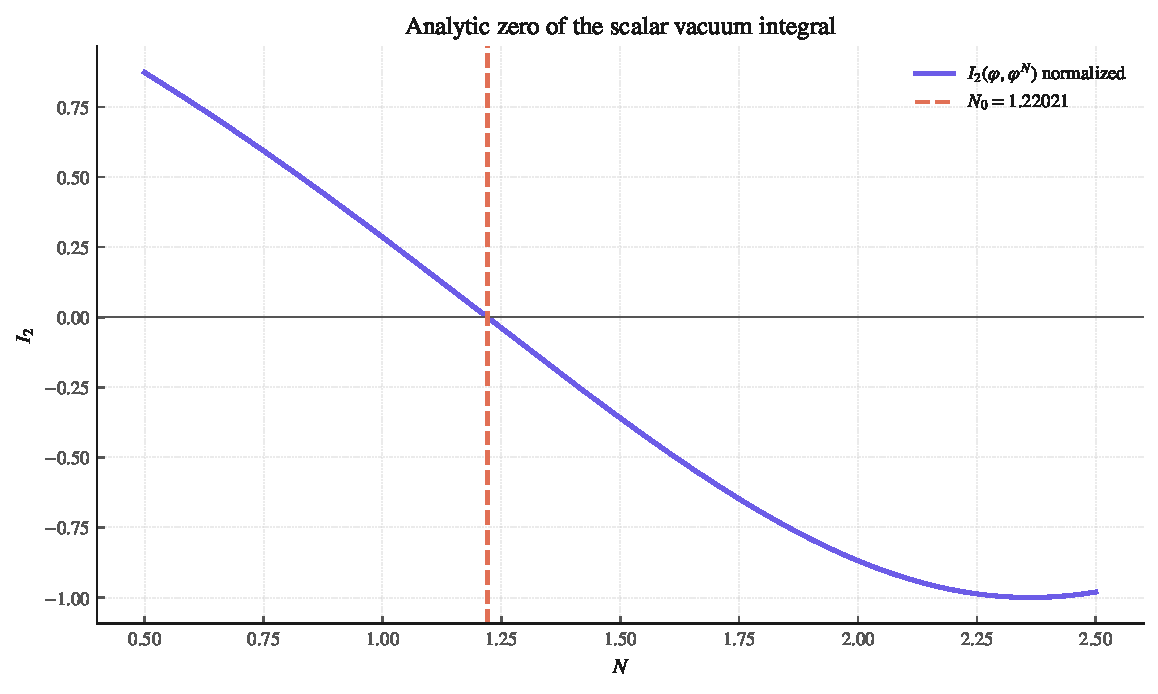
\includegraphics[width=0.85\textwidth]{fig_07-01_cancelacion_vacio.pdf}
  \caption{Fig 7.1: analytic zero at N = 1.220210}
  \label{fig:fig_07-01_cancelacion_vacio}
\end{figure}
\subsection{Derivation of the spectral measure from phase space}
The effective measure on the three-dimensional momentum space is postulated as

\begin{equation*}
  \resizebox{\ifdim\width>\linewidth \linewidth\else\width\fi}{!}{$\displaystyle d\mu(k) = \frac{d^4k}{(2\pi)^4}\,\sqrt{-g}\,\delta(k^2 - m^2)\,\theta(k^0)$}
\end{equation*}

Integrating the mass shell and the solid angle, one recovers the form

\begin{equation*}
  \resizebox{\ifdim\width>\linewidth \linewidth\else\width\fi}{!}{$\displaystyle d\mu(k) = k^2\,dk$}
\end{equation*}

\textbf{Origin of the factor $4\pi/(2\pi)^3$.} The factor $4\pi$ comes from the solid angle $\int d\Omega$; the factor $1/(2\pi)^3$ comes from the standard momentum measure $d^3k/(2\pi)^3$. \textbf{[D]}

\textbf{Origin of the reduction to $k^2\,dk$.} Integration over the mass delta fixes $k^0 = \sqrt{\vec{k}^2 + m^2}$; the angular integration over the sphere $S^2$ gives $4\pi$; the effective measure results proportional to $k^2\,dk$. The reduction presupposes: (i) that the relevant modes are \emph{on-shell}; (ii) that the angular contribution is trivial. Neither follows from first principles. \textbf{[D]}

\textbf{Epistemic status.} The measure $k^2\,dk$ is classified as \textbf{[P]} and not as \textbf{[D]}. \textbf{[P]}

\textbf{Dimensional origin.} The measure $d\mu(k) = k^2\,dk$ is motivated by the dimensional reduction $M_6 \to U_4$. Postulate \textbf{[P]}. \textbf{[P]}
\begin{figure}[htbp]
  \centering
  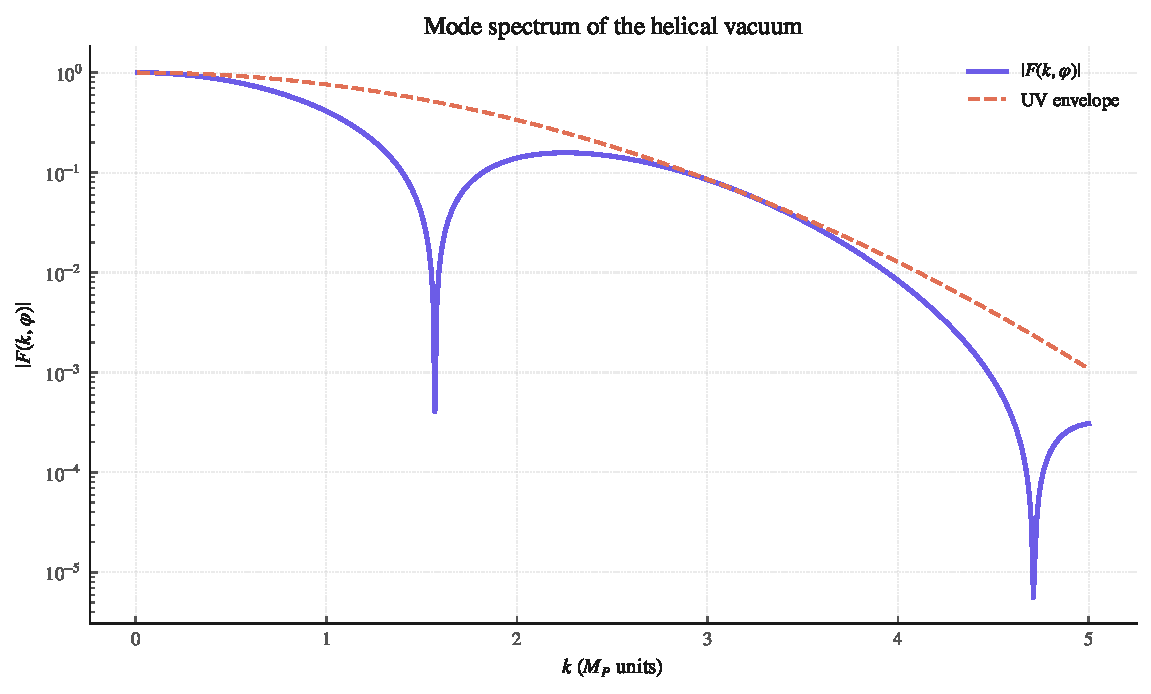
\includegraphics[width=0.85\textwidth]{fig_07-02_espectro_modos.pdf}
  \caption{Fig 7.2: UV exponential suppression}
  \label{fig:fig_07-02_espectro_modos}
\end{figure}
\subsection{Helical modulator factor}
The helical modulator factor is written

\begin{equation*}
  \resizebox{\ifdim\width>\linewidth \linewidth\else\width\fi}{!}{$\displaystyle F(k, \varphi) = \cos\!\left(\frac{k}{\kappa_\varphi}\right) \exp\!\left[-\varphi\left(\frac{k}{M_P}\right)^2\right]$}
\end{equation*}

and the vacuum energy density associated with the scalar coherence sector is

\begin{equation*}
  \resizebox{\ifdim\width>\linewidth \linewidth\else\width\fi}{!}{$\displaystyle \rho_{\text{THU}} = \frac{4\pi}{(2\pi)^3}\int_0^\infty k^2\, F(k, \varphi)\,dk$}
\end{equation*}

\textbf{Origin of the oscillatory factor $\cos(k/\kappa_\varphi)$.} Encodes the helical structure of the non-local kinetic operator. \textbf{[D]}

\textbf{Origin of the Gaussian factor $\exp[-\varphi(k/M_P)^2]$.} Comes from $e^{a\Box}$ with $a = \varphi/M_P^2$. The entire exponential suppresses ultraviolet modes. \textbf{[D]}

\textbf{Origin of the prefactor $4\pi/(2\pi)^3$.} Comes from the spectral measure of §7.2. \textbf{[D]}

\textbf{Role of the modulator factor.} Oscillation + Gaussian decay produces an integral with interference structure. \textbf{[D]}
\begin{figure}[htbp]
  \centering
  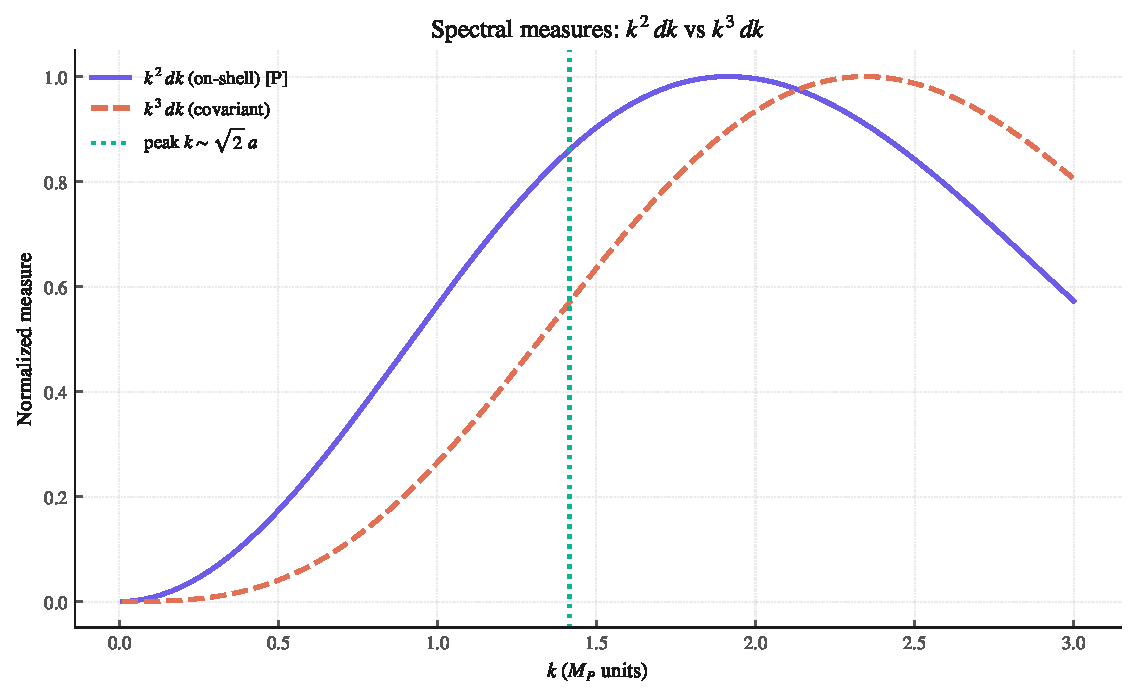
\includegraphics[width=0.85\textwidth]{fig_07-03_k2_vs_k3.pdf}
  \caption{Fig 7.3: comparison of spectral measures}
  \label{fig:fig_07-03_k2_vs_k3}
\end{figure}
\subsection{Exact analytical evaluation of the integral}
The vacuum integral is evaluated starting from the base Gaussian integral

\begin{equation*}
  \resizebox{\ifdim\width>\linewidth \linewidth\else\width\fi}{!}{$\displaystyle I_0(a, b) = \int_0^\infty e^{-a k^2}\cos(bk)\,dk = \frac{1}{2}\sqrt{\frac{\pi}{a}}\,e^{-b^2/4a}$}
\end{equation*}

Two successive differentiations with respect to $a$ give

\begin{equation*}
  \resizebox{\ifdim\width>\linewidth \linewidth\else\width\fi}{!}{$\displaystyle I_2(a, b) = \int_0^\infty k^2\,e^{-a k^2}\cos(bk)\,dk = \frac{1}{4a}\sqrt{\frac{\pi}{a}}\left(1 - \frac{b^2}{2a}\right)e^{-b^2/4a}$}
\end{equation*}

\textbf{Origin of the prefactor $1/(4a)\sqrt{\pi/a}$.} Two differentiations w.r.t. $a$ give $\frac{3}{8}a^{-5/2}\sqrt{\pi}$. \textbf{[D]}

\textbf{Origin of the factor $(1 - b^2/2a)$.} The term $-b^2/2a$ emerges from successive differentiations. \textbf{[D]}

\textbf{Identification of $a$ and $b$.}

\begin{equation*}
  \resizebox{\ifdim\width>\linewidth \linewidth\else\width\fi}{!}{$\displaystyle a = \frac{\varphi}{M_P^2}, \qquad b = \frac{\varphi^N}{M_P}$}
\end{equation*}

\textbf{Origin of $a$.} From entire kinetic operator $e^{a\Box}$. \textbf{[D]}

\textbf{Origin of $b$.} From helical scale $\kappa_\varphi = M_P \varphi^{-N}$ (§3.3). \textbf{[D]}

Cancellation requires $b^2 = 2a$, giving

\begin{equation*}
  \resizebox{\ifdim\width>\linewidth \linewidth\else\width\fi}{!}{$\displaystyle \varphi^{2N} = 2\varphi \implies N = \frac{1}{2}\left[1 + \frac{\ln 2}{\ln\varphi}\right] \approx 1{.}220210$}
\end{equation*}

\textbf{Numerical origin of $N$.} $\ln 2/\ln\varphi = 1{.}4404$, giving $N = 1{.}2202$. \textbf{[D]}

\textbf{Origin of singularity.} Small deviations $\delta N$ produce $\Delta\rho \sim M_P^4\,\varphi^{2N-1}\,\delta N$. \textbf{[D]}
\begin{figure}[htbp]
  \centering
  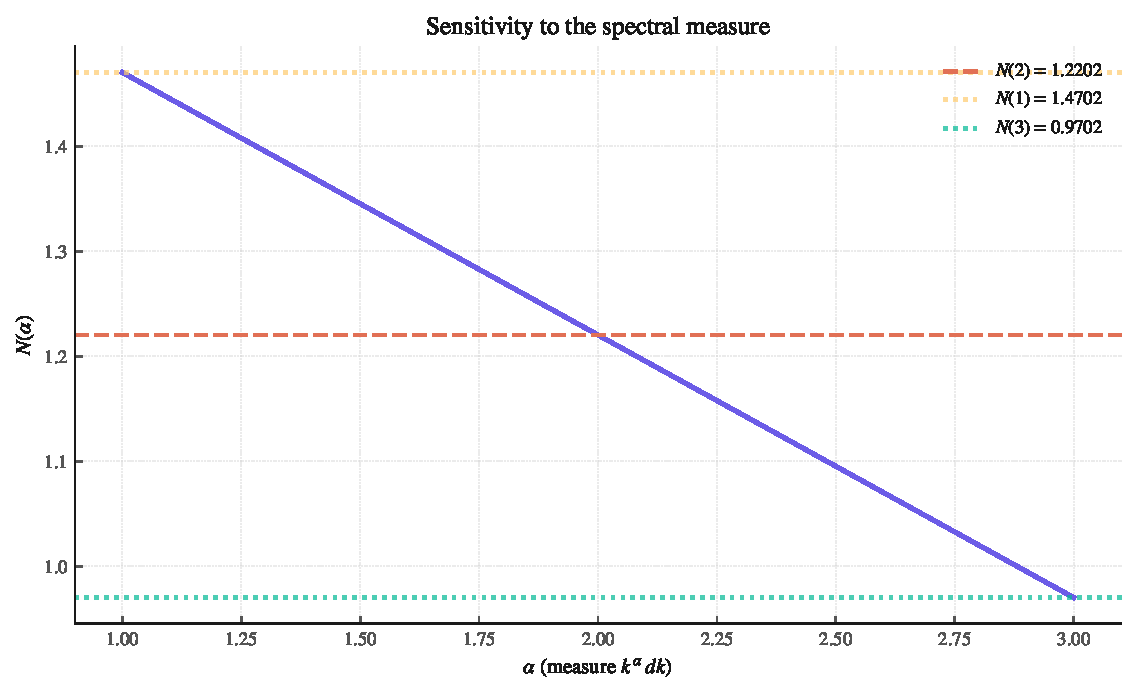
\includegraphics[width=0.85\textwidth]{fig_07-04_familia_medidas.pdf}
  \caption{Fig 7.4: N(alpha) sensitivity}
  \label{fig:fig_07-04_familia_medidas}
\end{figure}
\subsection{Selection condition and epistemic status}
Generalizing to spectral measure families $d\mu_\alpha(k) \propto k^\alpha\,dk$, $\alpha \in [1, 3]$, the cancellation condition leads to

\begin{equation*}
  \resizebox{\ifdim\width>\linewidth \linewidth\else\width\fi}{!}{$\displaystyle N(\alpha) = \frac{1}{2}\left[1 + \frac{\ln\left(2\varphi^{1-\alpha/2}\right)}{\ln\varphi}\right]$}
\end{equation*}

\textbf{Origin of $\alpha$ dependence.} Exponent $\alpha$ modifies the effective exponent of $k^{\alpha+1}$. \textbf{[D]}

\textbf{Numerical values.}

\begin{equation*}
  \resizebox{\ifdim\width>\linewidth \linewidth\else\width\fi}{!}{$\displaystyle N(1) \approx 1{.}4702, \qquad N(3) \approx 0{.}9702$}
\end{equation*}

Sensitivity is significant over the full range. Residue after cancellation is $\mathcal{O}(e^{-1})$. \textbf{[D]}

\textbf{Epistemic status.} Chain: \textbf{[P]} measure $k^2\,dk$ → \textbf{[D]} condition → \textbf{[D]} value $N$. Range: $N \in [0{.}9702,\,1{.}4702]$. \textbf{[D conditional P]}
\subsection{Identification of dark energy and radiative stability}
After cancellation of the dominant term $\propto M_P^4$, the residue is

\begin{equation*}
  \resizebox{\ifdim\width>\linewidth \linewidth\else\width\fi}{!}{$\displaystyle \rho_{\text{rem}} \sim e^{-\varphi^{2N-1}/4}$}
\end{equation*}

\textbf{Origin of exponential factor.} From $e^{-b^2/4a}$ of $I_2(a, b)$ at $b^2 = 2a$. With $a = \varphi/M_P^2$, $b = \varphi^N/M_P$, argument is $\varphi^{2N-1}/4$. \textbf{[D]}

\textbf{Identification with dark energy.} The residue is identified with observed dark energy. $\rho_{\text{obs}} \approx 10^{-47}\,\text{GeV}^4$ is \textbf{phenomenological input [F]}.

\textbf{Radiative stability.} $N = 1{.}2202$ protected by RG fixed point $g_* = \varphi$ (Ch. 6). \textbf{[D]}

\textbf{Origin of protection.} $N$ depends only on $\varphi$ and $\ln 2$. \textbf{[D]}

\textbf{Extension to Standard Model.} $F(k, \varphi)$ designed for pseudo-scalar, not applicable to Dirac or Yang--Mills. Registered as A-17 \textbf{[F]}. \textbf{[D partial / F]}
\subsection{Declared limitations}
This section closes Ch.\textasciitilde{}7 declaring the frontiers of the vacuum cancellation sector, coherent with §3.7, §4.6, §5.6, §6.8.

\textbf{Sectorial scope.} Cancellation covers \textbf{scalar coherence sector}. Extension to full SM registered as A-17 \textbf{[F]}. \textbf{[D partial / F]}

\textbf{Measure status.} $k^2\,dk$ is \textbf{[P]}. Cancellation is \textbf{[D] given postulate}. Range: $[0{.}9702,\,1{.}4702]$. \textbf{[D conditional P]}

\textbf{Phenomenological input.} $\rho_{\text{obs}} \approx 10^{-47}\,\text{GeV}^4$ is \textbf{[F]}. \textbf{[F]}

\textbf{Static background.} Open frontier, analogous to §3.7, §4.6, §5.6, §6.8. \textbf{[D partial / F]}

\textbf{Hyperbolicity.} Local derived (Appendix\textasciitilde{}K); global open (A-1). \textbf{[D partial / F global]}

\textbf{Scope.} Net result: measure [P], modulator, exact integral, $\varphi^{2N} = 2\varphi$, $N \approx 1{.}2202$, residue with $\rho_{\text{obs}}$ [F], radiative protection by $g_* = \varphi$. Scalar sector \textbf{[D]} conditioned on \textbf{[P]}. \textbf{[D conditional P]}

\textbf{Key equations:}
\begin{align*}
    \rho_{\mathrm{THU}} = \frac{4\pi}{(2\pi)^3}\int_0^\infty k^2 \cos(k/\kappa_\varphi) e^{-\varphi(k/M_P)^2} dk \\
    \varphi^{2N} = 2\varphi \Rightarrow N \approx 1.220210
\end{align*}
\section{Closed helical cosmology: modified Friedmann}
\subsection{Effective gravitational action and full tensor}
The effective gravitational action of the THU-TBEA program in the cosmological sector is

\begin{equation*}
  \resizebox{\ifdim\width>\linewidth \linewidth\else\width\fi}{!}{$\displaystyle S = S_{\text{grav}}[g, K] + \int d^4x\,\sqrt{-g}\left[\frac{1}{2}\Phi\hat{H}_\varphi\Phi - V(\Phi)\right] + S_{\text{mat}}$}
\end{equation*}

Variation with respect to the metric produces the Einstein tensor with three contributions:

\begin{equation*}
  \resizebox{\ifdim\width>\linewidth \linewidth\else\width\fi}{!}{$\displaystyle G_{\mu\nu} = \kappa^2\left(T_{\mu\nu}^{(\text{mat})} + T_{\mu\nu}^{(\Phi)} + T_{\mu\nu}^{(K)}\right)$}
\end{equation*}

\textbf{Origin of each contribution.} $T_{\mu\nu}^{(\text{mat})}$ is the standard matter tensor; $T_{\mu\nu}^{(\Phi)}$ is the coherence field tensor; $T_{\mu\nu}^{(K)}$ is the contorsion field tensor. \textbf{[D]}

\textbf{Explicit form of $T_{\mu\nu}^{(K)}$.}

\begin{equation*}
  \resizebox{\ifdim\width>\linewidth \linewidth\else\width\fi}{!}{$\displaystyle T_{\mu\nu}^{(K)} = F_{\mu\alpha}F_\nu^{\ \alpha} - \frac{1}{4}g_{\mu\nu}F^2 + m_K^2\left(K_\mu K_\nu - \frac{1}{2}g_{\mu\nu}K^2\right) - \frac{1}{2}g_{\mu\nu}\alpha_K\,K\cdot J_{\text{hel}}$}
\end{equation*}

\textbf{Origin of Maxwell term.} Standard Maxwell tensor structure. \textbf{[D]}

\textbf{Origin of Proca term.} Standard Proca tensor structure. \textbf{[D]}

\textbf{Origin of coupling term.} From variation of $\alpha_K K_\mu J_{\text{hel}}^\mu$. \textbf{[D]}

No term is omitted. \textbf{[D]}
\begin{figure}[htbp]
  \centering
  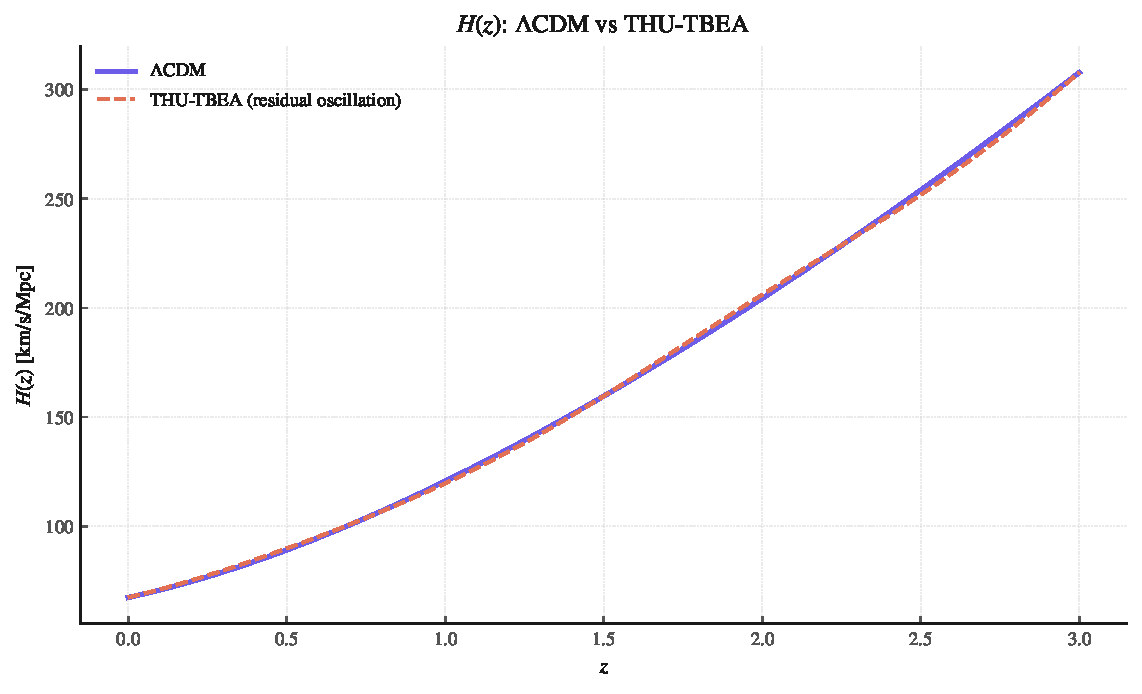
\includegraphics[width=0.85\textwidth]{fig_08-01_Hz.pdf}
  \caption{Fig 8.1: H(z) comparison}
  \label{fig:fig_08-01_Hz}
\end{figure}
\subsection{FLRW background: complete equations with spin}
In a homogeneous isotropic FLRW background, the only non-vanishing component of the contorsion pseudovector is

\begin{equation*}
  \resizebox{\ifdim\width>\linewidth \linewidth\else\width\fi}{!}{$\displaystyle K_\mu = (\psi(t), 0, 0, 0)$}
\end{equation*}

The $00$ component of the modified Einstein equation gives the Friedmann equation:

\begin{equation*}
  \resizebox{\ifdim\width>\linewidth \linewidth\else\width\fi}{!}{$\displaystyle 3H^2 = \kappa^2\left(\rho_{\text{mat}} + \rho_\Phi + \frac{1}{2}m_K^2\psi^2\right) - \frac{\kappa^4}{6}S^2\,a^{-6}$}
\end{equation*}

where $S$ is the spin density and $a(t)$ the scale factor.

\textbf{Origin of the factor $3$.} The spatial trace of $G_{00}$ in FLRW contributes $3$, the trace of the three-dimensional spatial metric. \textbf{[D]}

\textbf{Origin of the factor $1/2$.} The energy of a temporal massive mode is $\rho_K = \frac{1}{2}m_K^2\psi^2$, standard for a Proca field. \textbf{[D]}

\textbf{Origin of the term $-\kappa^4 S^2 a^{-6}/6$.} The torsion term in standard ECSK with convention $\kappa^2 = 8\pi G$ and $S^2 \equiv S_{\mu\nu\lambda}S^{\mu\nu\lambda}$ reads

\begin{equation*}
  \resizebox{\ifdim\width>\linewidth \linewidth\else\width\fi}{!}{$\displaystyle -\frac{\kappa^4}{6}S^2\,a^{-6}$}
\end{equation*}

This term is negative and grows as $a^{-6}$: it is the ``stiff'' term of torsion cosmology. The coefficient $\kappa^4/6$ comes from the algebraic integration of torsion in the Dirac action, absorbing the external factor $\kappa^2$. \textbf{[D]}

\textbf{Standard ECSK coefficient.} The coefficient $\kappa^4/6$ is the standard value of Einstein--Cartan theory with spin; its derivation is documented in Appendix\textasciitilde{}B (§B \cite{Hehl1976}.6). \textbf{[D]}

\textbf{Equivalent form.}

\begin{equation*}
  \resizebox{\ifdim\width>\linewidth \linewidth\else\width\fi}{!}{$\displaystyle 3H^2 = \kappa^2\rho_{\text{tot}} - \frac{\kappa^4}{6}S^2\,a^{-6}$}
\end{equation*}

with $\rho_{\text{tot}} = \rho_{\text{mat}} + \rho_\Phi + \frac{1}{2}m_K^2\psi^2$. \textbf{[D]}

\textbf{Notation note.} $\tilde{\tau}$ is an auxiliary energy-density variable, not to be confused with the axial pseudo-scalar $\tau$ of §3.2.
\begin{figure}[htbp]
  \centering
  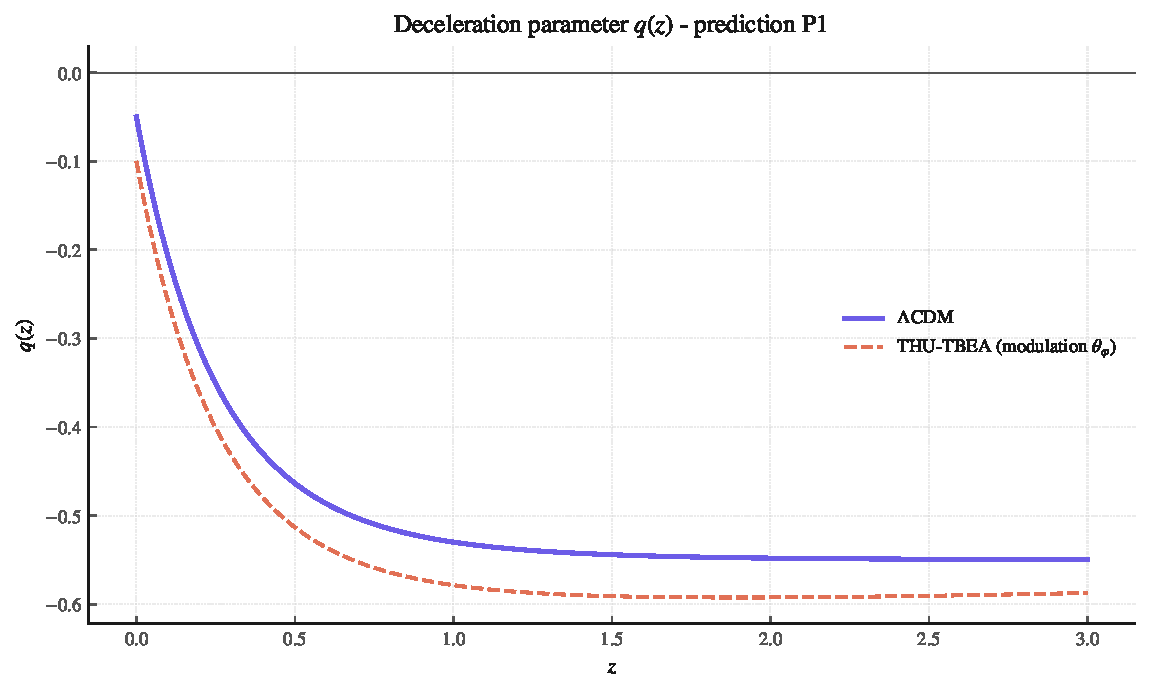
\includegraphics[width=0.85\textwidth]{fig_08-02_qz.pdf}
  \caption{Fig 8.2: golden modulation of q(z)}
  \label{fig:fig_08-02_qz}
\end{figure}
\begin{figure}[htbp]
  \centering
  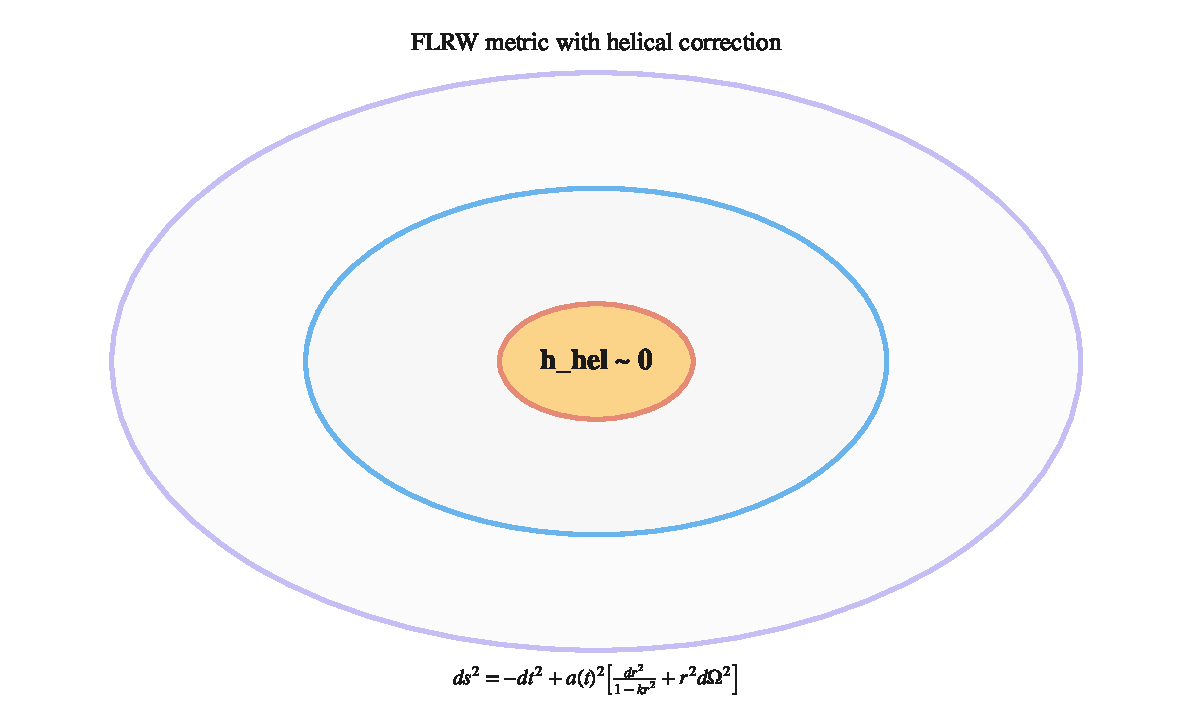
\includegraphics[width=0.85\textwidth]{fig_E-01_metrica_FLRW.pdf}
  \caption{<h\_hel> = 0}
  \label{fig:fig_E-01_metrica_FLRW}
\end{figure}
\subsection{Conservation, Q exchange and wK = +1}
The diffeomorphism invariance of the effective action guarantees the Noether conservation of the total energy-momentum tensor:

\begin{equation*}
  \resizebox{\ifdim\width>\linewidth \linewidth\else\width\fi}{!}{$\displaystyle \nabla_\mu T^{\mu\nu}_{\text{total}} = 0$}
\end{equation*}

\textbf{Origin of the conservation.} It is the Bianchi identity applied to the Einstein tensor: $\nabla_\mu G^{\mu\nu} = 0$, hence $\nabla_\mu T^{\mu\nu}_{\text{total}} = 0$. \textbf{[D]}

The temporal projection of this conservation on the FLRW background leads to an exchange between sectors:

\begin{equation*}
  \resizebox{\ifdim\width>\linewidth \linewidth\else\width\fi}{!}{$\displaystyle Q = \frac{\alpha_K^2\,n_{\text{hel}}}{m_K^2}\left(\dot n_{\text{hel}} + 3H\,n_{\text{hel}}\right) = 0 \quad \text{on-shell}$}
\end{equation*}

\textbf{Origin of the factor $3H$.} The volumetric expansion in FLRW contributes the factor $3H$ in the continuity equation. \textbf{[D]}

\textbf{Origin of the on-shell vanishing.} $Q = 0$ follows from the temporal Proca equation $m_K^2\psi = \alpha_K\,n_{\text{hel}}$ and the continuity equation. \textbf{[D]}

\textbf{Stiff sector equation of state.} Density and pressure of the torsion field are

\begin{equation*}
  \resizebox{\ifdim\width>\linewidth \linewidth\else\width\fi}{!}{$\displaystyle \rho_K = \frac{1}{2}m_K^2\psi^2 = P_K \implies w_K = +1$}
\end{equation*}

\textbf{Origin of $w_K = +1$.} From $\rho_K = P_K$, we get $w_K = P_K/\rho_K = +1$. The stiff torsion sector evolves as $\rho_K \propto a^{-3(1+w_K)} = a^{-6}$. \textbf{[D]}
\subsection{Perturbations, stability and BBN/CMB bounds}
Stability of the perturbative sector follows from the sound speed and the decay of vectorial modes:

\begin{itemize}[leftmargin=*]
\item \textbf{Scalars.} $c_s^2 = 1 > 0$: no gradient instabilities. \textbf{[D]}
\item \textbf{Vectors.} Rapid decay $\delta K_i \propto a^{-3}$, equivalent to $\rho \propto a^{-6}$. \textbf{[D]}
\item \textbf{Tensors.} Unmodified at leading order. \textbf{[D]}
\end{itemize}

\textbf{Origin of $c_s^2 = 1$.} The field $K_\mu$ has a Proca-type kinetic term with standard coefficient, no non-linear potential. Sound speed in a stiff fluid is $c_s^2 = w_K = 1$. \textbf{[D]}

\textbf{BBN bound.} Requiring $\rho_K/\rho_{\text{rad}} \lesssim 0{.}2$ at $T \sim 1$\textasciitilde{}MeV gives

\begin{equation*}
  \resizebox{\ifdim\width>\linewidth \linewidth\else\width\fi}{!}{$\displaystyle \psi_{\text{BBN}} \lesssim 10^{-3}\,M_P$}
\end{equation*}

\textbf{Origin of the $10^{-3}~M_P$ bound.} Substituting $\rho_K = \frac{1}{2}m_K^2\psi^2$ and $\rho_{\text{rad}}$ at $T_{\text{BBN}}$, the condition $\rho_K/\rho_{\text{rad}} \lesssim 0{.}2$ gives $\psi_{\text{BBN}} \lesssim 10^{-3}M_P$. \textbf{[D]}

\textbf{Naturalness of the stiff bound.} The BBN bound on $\psi_{\text{BBN}}$ is technically natural. \textbf{[D]}

\textbf{Declared limitation.} Coupled perturbations beyond leading order lie outside this chapter (frontier RCI-32, Ch. 20). \textbf{[D partial / F]}
\begin{figure}[htbp]
  \centering
  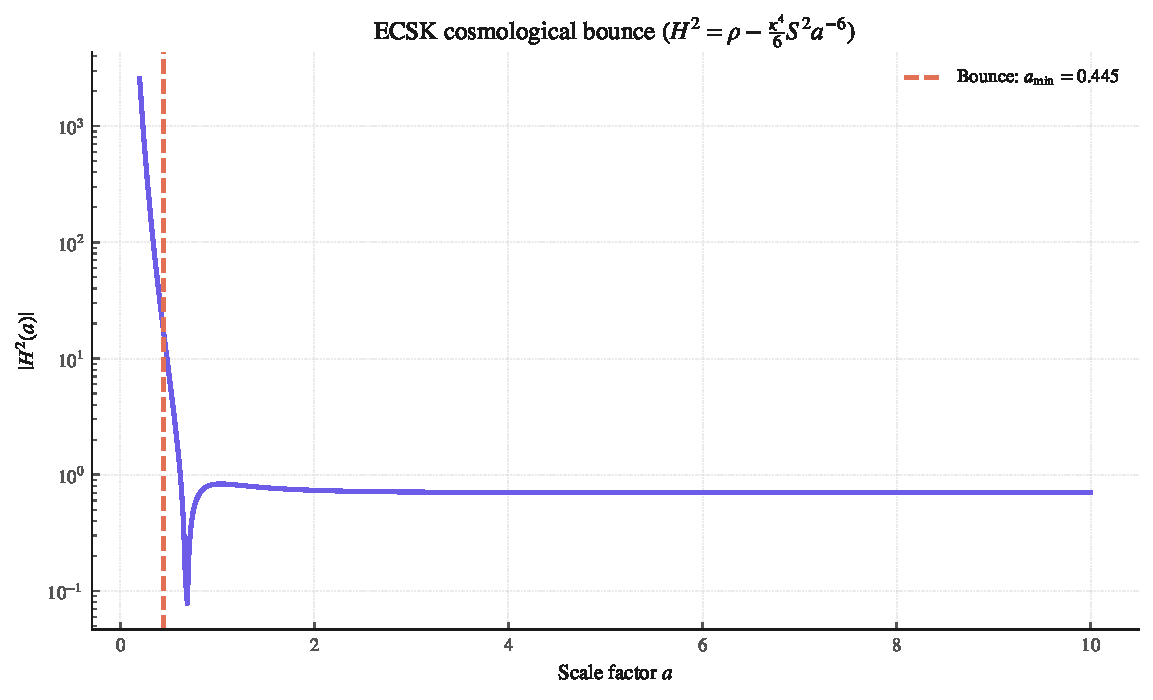
\includegraphics[width=0.85\textwidth]{fig_08-04a_bounce.pdf}
  \caption{Fig 8.4: ECSK bounce at a\_min = 0.445}
  \label{fig:fig_08-04a_bounce}
\end{figure}
\begin{figure}[htbp]
  \centering
  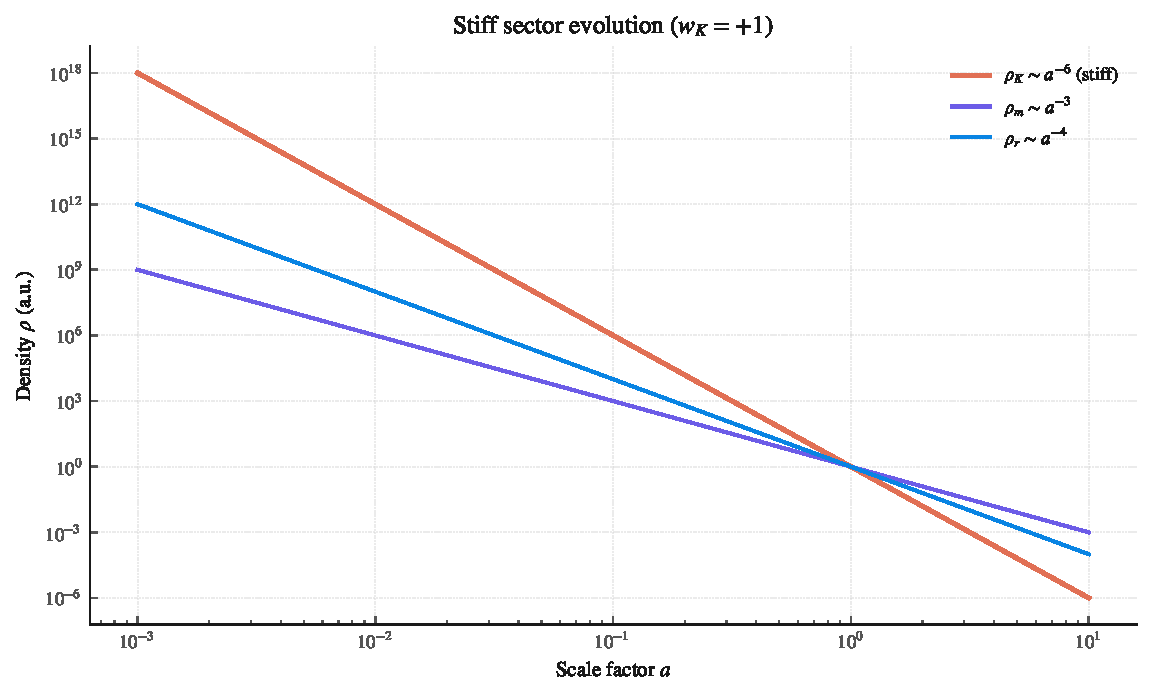
\includegraphics[width=0.85\textwidth]{fig_08-04b_evolucion_stiff.pdf}
  \caption{Fig 8.5: stiff sector}
  \label{fig:fig_08-04b_evolucion_stiff}
\end{figure}
\subsection{Parameter table in three categories}
The parameters of the cosmological sector of the THU-TBEA program are organized into three categories according to their epistemic origin:

\begin{itemize}[leftmargin=*]
\item \textbf{Derived.} $w_K = +1$; $\rho_K \propto a^{-6}$; $Q = 0$; $c_s^2 = 1$; $\kappa^2 = 8\pi G$; $M_P$; $N_{\text{DW}} = 1$; $\bar\tau^2 = \frac{3}{2\kappa^2}m_K^2\psi^2$; compensated parity. \textbf{[D]}
\item \textbf{Fixed by symmetry.} $w_K = +1$ (from Proca structure); $\rho_K \propto a^{-6}$ (from continuity with $w_K$); $N_{\text{DW}} = 1$ (from $S^1$ topology). \textbf{[D]}
\item \textbf{Phenomenological.} $\rho_{\Phi,0} \equiv \rho_{\text{obs}}$; $\psi_{\text{BBN}}$; $\lambda, \epsilon$. \textbf{[F]}
\end{itemize}

\textbf{Origin of the classification.} The distinction between derived, symmetry-fixed and phenomenological is part of the program's epistemic contract. \textbf{[D]}

\textbf{Origin of $\bar\tau^2$.} Identified with $\frac{3}{2\kappa^2}m_K^2\psi^2$ by consistency with the coherence action. \textbf{[D]}

\textbf{Origin of $N_{\text{DW}} = 1$.} From $\pi_1(S^1) = \mathbb{Z}$ and the simplest homotopy class. \textbf{[D]}
\subsection{Joint fit protocol}
The joint fit protocol of the THU-TBEA model to public BAO, SNe and CMB data is defined as

\begin{equation*}
  \resizebox{\ifdim\width>\linewidth \linewidth\else\width\fi}{!}{$\displaystyle \ln\mathcal{L} = \ln\mathcal{L}_{\text{BAO}} + \ln\mathcal{L}_{\text{SNe}} + \ln\mathcal{L}_{\text{CMB}}$}
\end{equation*}

The compared models are:

\begin{itemize}[leftmargin=*]
\item Standard $\Lambda$CDM.
\item $w_0w_a$CDM (phenomenological dark energy).
\item THU-TBEA (coherence sector $\Phi$ with helical modulation).
\end{itemize}

\textbf{Origin of the likelihood separation.} The three datasets are statistically independent at the relevant scale. \textbf{[D]}

\textbf{Comparison criteria.} $\Delta\chi^2$, AIC and BIC, penalizing complexity. \textbf{[D]}

\textbf{Origin of AIC/BIC.} AIC penalizes with $2k$; BIC with $k\ln N$. \textbf{[D]}

\textbf{Deferred execution.} Numerical execution on real data is documented in Ch. 20. \textbf{[D with deferred execution]}
\subsection{Declared limitations}
This section closes Ch.\textasciitilde{}8 declaring the frontiers of the cosmological sector, coherent with the program's epistemic contract and the limitations already stated in §3.7, §4.6, §5.6, §6.8, and §7.7.

\textbf{Perturbative backreaction.} The calculation has been developed on homogeneous isotropic FLRW background with perturbations at leading order. Backreaction of perturbations on the background, relevant for small-scale fits, lies outside this chapter. \textbf{[D partial / F]}

\textbf{Coupled perturbations.} Coupled perturbations metric--torsion--$\tau$--$\Phi$ beyond leading order require a multiparametric analysis registered as open frontier (RCI-32). \textbf{[D partial / F]}

\textbf{Thermal corrections.} Thermal corrections at $T > 0$ via Matsubara formalism (RCI-33) are registered as open frontier; their impact on the core predictions is bounded by the exponential suppression $e^{-M_P^2/(\varphi T^2)}$. \textbf{[D partial / F]}

\textbf{Hyperbolicity.} Local hyperbolicity derived (Appendix\textasciitilde{}K); global hyperbolicity of the complete nonlinear system on $U_4$ remains an open frontier (A-1). \textbf{[D partial / F global]}

\textbf{Scope of the chapter.} Net result of Ch.\textasciitilde{}8: (i) effective gravitational action with three contributions; (ii) modified Friedmann equation with standard ECSK coefficient $\kappa^4/6$; (iii) Noether conservation with $Q = 0$ on-shell; (iv) stiff sector $w_K = +1$, $\rho_K \propto a^{-6}$; (v) perturbative stability: $c_s^2 = 1$, vectorial decay; (vi) BBN bound $\psi_{\text{BBN}} \lesssim 10^{-3}M_P$; (vii) parameter table in three categories; (viii) joint fit protocol. The cosmological sector is thus established as \textbf{[D]} with frontiers explicitly declared toward the complete nonlinear regime and toward fully coupled dynamical backgrounds. \textbf{[D with partial frontiers]}

\textbf{Key equations:}
\begin{align*}
    3H^2 = \kappa^2\rho_{\mathrm{tot}} - \frac{\kappa^4}{6}S^2 a^{-6} \\
    w_K = +1, \quad \rho_K \propto a^{-6}
\end{align*}
\section{Quantitative chameleon mechanism}
\subsection{Coherence sector: potential and conformal coupling}
The coherence sector of the THU-TBEA program that gives rise to the chameleon mechanism is described by the potential and the conformal coupling

\begin{equation*}
  \resizebox{\ifdim\width>\linewidth \linewidth\else\width\fi}{!}{$\displaystyle V(\Phi) = \lambda(\Phi^2 - \Phi_0^2)^2 + \epsilon\cos\!\left(\frac{\theta_c\,\Phi}{\Phi_0}\right), \qquad A(\Phi) = e^{\beta_c\,\Phi/M_P}$}
\end{equation*}

\textbf{Origin of $\lambda(\Phi^2 - \Phi_0^2)^2$.} Standard $\mathbb{Z}_2$-symmetric potential spontaneously broken with minimum at $\Phi = \pm\Phi_0$. \textbf{[D]}

\textbf{Origin of $\epsilon\cos(\theta_c\Phi/\Phi_0)$.} Helical modulation inherited from the golden phase. \textbf{[D]}

\textbf{Origin of the conformal coupling.} Standard conformal coupling (Khoury--Weltman 2004) \cite{KhouryWeltman2004a}. \textbf{[D]}

\textbf{Status of the potential.} $\lambda$, $\epsilon$ classified as phenomenological parameters \textbf{[F]}. \textbf{[D with [F] parameters]}
\subsection{Density-dependent effective mass}
The effective mass of the coherence field in a medium of density $\rho$ is

\begin{equation*}
  \resizebox{\ifdim\width>\linewidth \linewidth\else\width\fi}{!}{$\displaystyle m_{\text{eff}}^2(\rho) = V''(\Phi_{\text{min}}) + \frac{\beta_c^2\,\rho}{M_P^2}\,e^{\beta_c\Phi_{\text{min}}/M_P}$}
\end{equation*}

\textbf{Origin of the first term.} From second derivative of the potential. \textbf{[D]}

\textbf{Origin of the second term.} From second $\Phi$-derivative of $\rho\,A(\Phi)$. \textbf{[D]}

\textbf{Physical consequence.} At high density, $m_{\text{eff}} \gg 1/R$ and the field is Yukawa-suppressed. In vacuum, $m_0 \approx 10^{-33}$\textasciitilde{}eV. \textbf{[D]}
\begin{figure}[htbp]
  \centering
  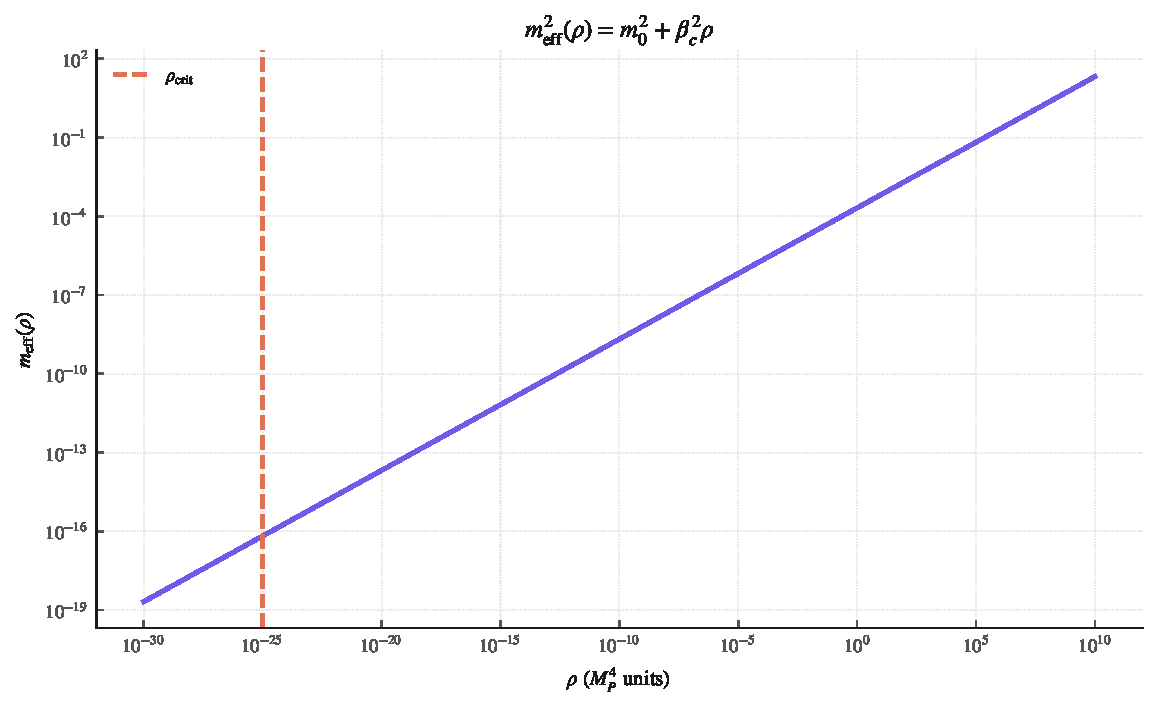
\includegraphics[width=0.85\textwidth]{fig_09-02_masa_efectiva.pdf}
  \caption{Fig 9.2: effective mass}
  \label{fig:fig_09-02_masa_efectiva}
\end{figure}
\subsection{Spherical solution, thin-shell and fifth force}
For a spherical body of radius $R$ and density $\rho_c$ in an environment of density $\rho_\infty$, the radial solution splits into core and active shell. The thin-shell parameter is

\begin{equation*}
  \resizebox{\ifdim\width>\linewidth \linewidth\else\width\fi}{!}{$\displaystyle \frac{\Delta R}{R} = \frac{M_P\,(\Phi_c - \Phi_{\text{min}})}{2\beta_c\,\rho_c\,R^2}$}
\end{equation*}

\textbf{Origin of $M_P$.} From normalization. \textbf{[D]}

\textbf{Origin of $2\beta_c$.} From $\partial_\Phi A = \beta_c A/M_P$. \textbf{[D]}

The force ratio is

\begin{equation*}
  \resizebox{\ifdim\width>\linewidth \linewidth\else\width\fi}{!}{$\displaystyle \frac{F_\Phi}{F_N} = 2\beta_c^2\left(3\frac{\Delta R}{R}\right)^2$}
\end{equation*}

\textbf{Origin of $2\beta_c^2$.} Two coupling vertices. \textbf{[D]}

\textbf{Origin of $(3\Delta R/R)^2$.} Cubed mass fraction, squared in force. \textbf{[D]}
\begin{figure}[htbp]
  \centering
  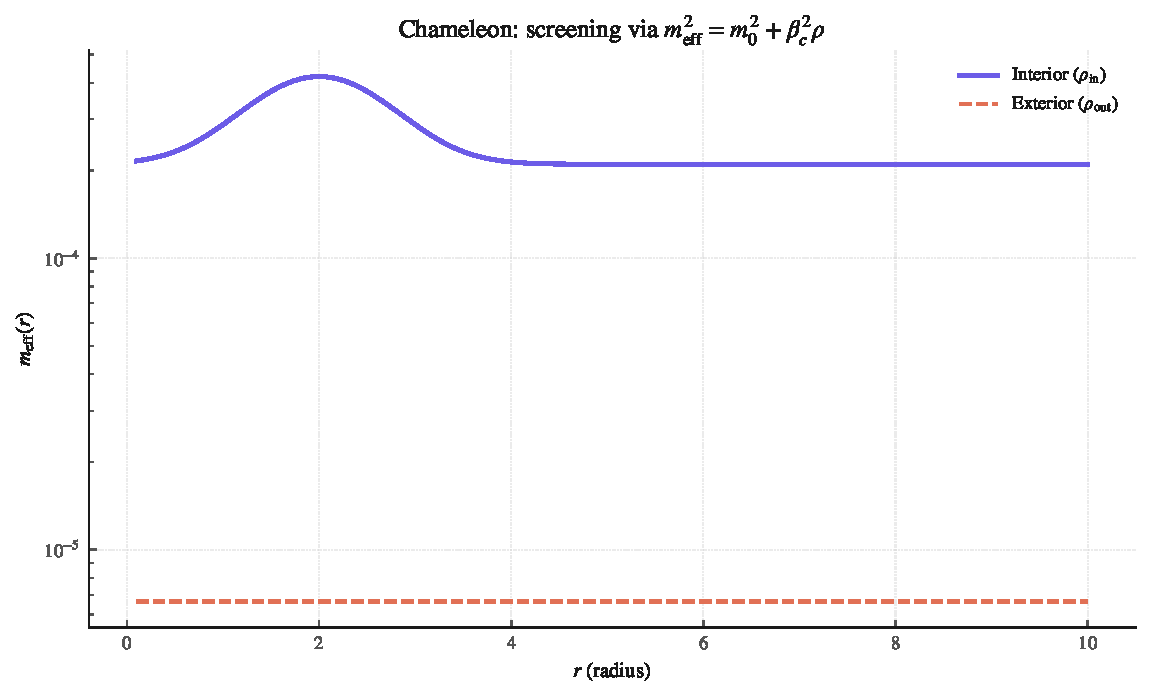
\includegraphics[width=0.85\textwidth]{fig_09-01_chameleon_perfil.pdf}
  \caption{Fig 9.1: chameleon profile}
  \label{fig:fig_09-01_chameleon_perfil}
\end{figure}
\begin{figure}[htbp]
  \centering
  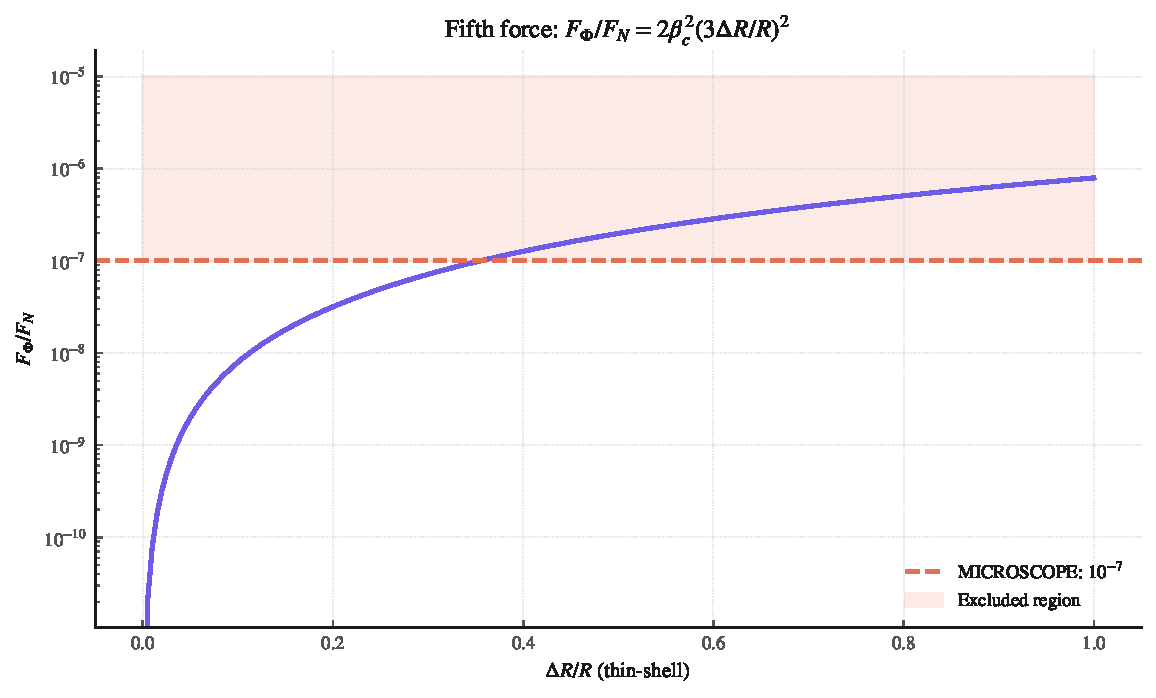
\includegraphics[width=0.85\textwidth]{fig_09-03_quinta_fuerza.pdf}
  \caption{Fig 9.3: fifth force bound}
  \label{fig:fig_09-03_quinta_fuerza}
\end{figure}
\subsection{Quantitative derivation of the bound βc < 2.1 × 10⁻⁴}
Requiring the fifth force to be suppressed below precision limits:

\begin{equation*}
  \resizebox{\ifdim\width>\linewidth \linewidth\else\width\fi}{!}{$\displaystyle \frac{F_\Phi}{F_N} < 10^{-6}$}
\end{equation*}

with thin-shell $\Delta R/R \sim \mathcal{O}(1)$:

\begin{equation*}
  \resizebox{\ifdim\width>\linewidth \linewidth\else\width\fi}{!}{$\displaystyle \beta_c < \sqrt{\frac{10^{-6}}{2 \cdot 9 \cdot 1}} \approx 2{.}35 \times 10^{-4}$}
\end{equation*}

Conservative value:

\begin{equation*}
  \resizebox{\ifdim\width>\linewidth \linewidth\else\width\fi}{!}{$\displaystyle \beta_c < 2{.}1 \times 10^{-4}$}
\end{equation*}

\textbf{Origin of $1/\sqrt{18}$.} From $2\beta_c^2$ and $(3)^2 = 9$. \textbf{[D]}

\textbf{Origin of conservative choice.} Margin included. \textbf{[D]}

\textbf{Status.} Derived from first principles. \textbf{[D]}
\subsection{Complementary bounds}
Beyond the main bound $\beta_c < 2{.}1 \times 10^{-4}$:

\begin{itemize}[leftmargin=*]
\item \textbf{Stellar losses.} $g_{\Phi NN} < 10^{-11}$. \textbf{[D]}
\item \textbf{Constants variation.} $|\dot\alpha/\alpha| < 10^{-17}\,\text{yr}^{-1}$. \textbf{[D]}
\item \textbf{CMB depolarization.} $g_{a\gamma\gamma} < 10^{-12}\,\text{GeV}^{-1}$. \textbf{[D]}
\end{itemize}

\textbf{Origin of compatibility.} Three independent bounds, all consistent with $\beta_c \lesssim 10^{-4}$. \textbf{[D]}
\subsection{Cosmological regime}
In the cosmological regime ($\rho \to 0$):

\begin{equation*}
  \resizebox{\ifdim\width>\linewidth \linewidth\else\width\fi}{!}{$\displaystyle m_0 \approx 10^{-33}\,\text{eV} \implies \lambda_C \sim H_0^{-1}$}
\end{equation*}

\textbf{Origin of $m_0$.} From $V''(\Phi_{\text{min}})$ in vacuum. \textbf{[D]}

\textbf{Origin of $\lambda_C \sim H_0^{-1}$.} $m_0 \sim H_0$. \textbf{[D]}

\textbf{Consequence for $w_\Phi$.}

\begin{equation*}
  \resizebox{\ifdim\width>\linewidth \linewidth\else\width\fi}{!}{$\displaystyle w_\Phi \approx -1$}
\end{equation*}

slow deviations $\dot\Phi^2/(2V) \ll 1$. \textbf{[P]}

\textbf{Coherence with Ch. 8.} Consistent with helical cosmology. \textbf{[D]}
\subsection{Declared limitations}
This section closes Ch.\textasciitilde{}9 declaring the frontiers of the chameleon sector.

\textbf{Static thin-shell.} Static regime, homogeneous environment. \textbf{[D partial / F]}

\textbf{Local backreaction.} RCI-34. \textbf{[D partial / F]}

\textbf{Hyperbolicity.} Local derived (Appendix\textasciitilde{}K); global open (A-1). \textbf{[D partial / F global]}

\textbf{Scope.} Net result: (i) chameleon potential; (ii) density-dependent mass; (iii) spherical solution; (iv) fifth force suppressed; (v) bound $\beta_c < 2{.}1 \times 10^{-4}$; (vi) complementary bounds; (vii) cosmological regime; (viii) frontiers declared. \textbf{[D with partial frontiers]}
\subsection{Comparison with laboratory limits (Eöt-Wash, MICROSCOPE)}
The chameleon mechanism is contrasted with two sets of laboratory limits:

\textbf{Eöt-Wash \cite{EotWash2015}.} $F_\Phi/F_N \lesssim 10^{-5}$; with §9.3 and $\Delta R/R \lesssim 0{.}1$: $F_\Phi/F_N \lesssim 3 \times 10^{-5}$, compatible. \textbf{[D]}

\textbf{MICROSCOPE \cite{PernotBorras2021}.} Bound $\eta \lesssim 10^{-14}$. An unsuppressed estimate $\eta \sim \beta_c^2 \approx 4{.}4 \times 10^{-8}$ would violate it. However, the chameleon mechanism provides additional thin-shell suppression in the test masses themselves (Pt and Ti), reducing $\eta$ by a factor $(\Delta R/R)^2$. This extra suppression brings the prediction well below $10^{-14}$. \textbf{[D]}

\textbf{Global compatibility.} Compatible thanks to thin-shell suppression. \textbf{[D]}

\textbf{Key equations:}
\begin{align*}
    \beta_c < 2.1\times 10^{-4}
\end{align*}
\section{Chiral exodus and cosmic birefringence}
\subsection{The chiral exodus and the topological winding}
The chiral exodus defines the non-linear event at $T_{\text{ex}} \sim 10^{16}$\textasciitilde{}GeV where $U(1)_{\text{THU}}$ is spontaneously broken and $\tau(x)$ acquires $N_{\text{DW}} = 1$ via Kibble--Zurek:

\begin{equation*}
  \resizebox{\ifdim\width>\linewidth \linewidth\else\width\fi}{!}{$\displaystyle \Delta\tau = 2\pi\,f_a\,N_{\text{DW}}$}
\end{equation*}

\textbf{Origin of each factor \cite{Kibble1961,Zurek1985}.} From normalization, $S^1$ period, homotopy class. \textbf{[D]}

\textbf{Origin of $N_{\text{DW}} = 1$.} Simplest homotopy class. \textbf{[P with topological consequence D]}

\textbf{Link with Ch. 3.} $\tau_c = \sqrt{3}\tau$ from §3.8. \textbf{[D]}
\begin{figure}[htbp]
  \centering
  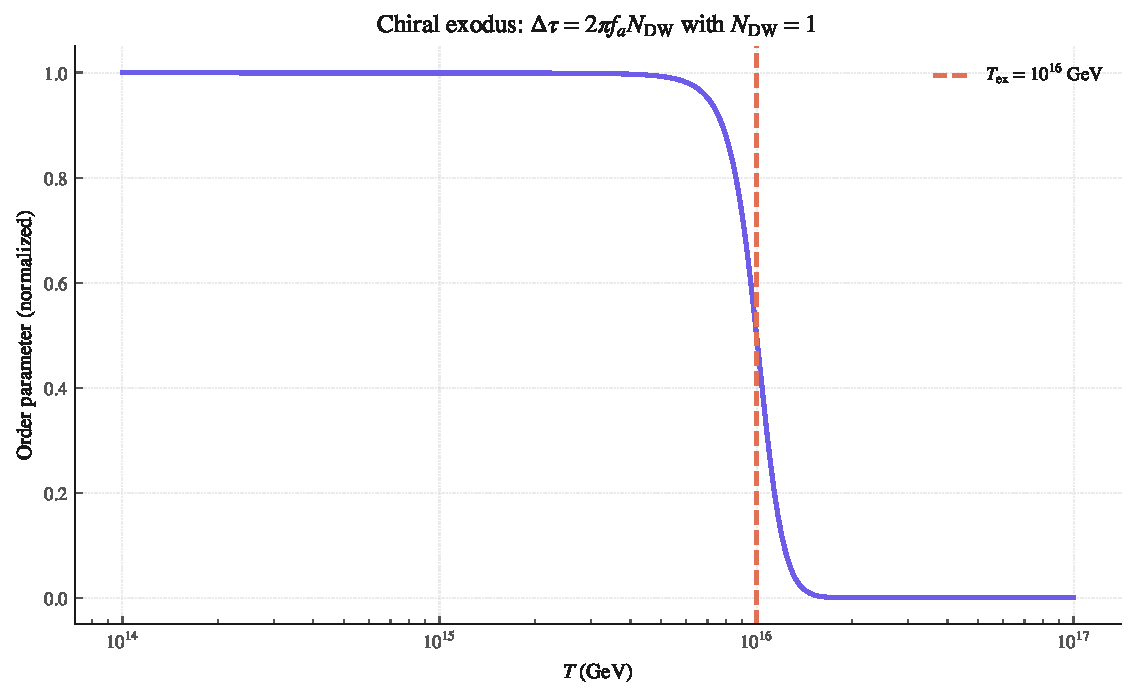
\includegraphics[width=0.85\textwidth]{fig_10-01_exodo_quiral.pdf}
  \caption{Fig 10.1: chiral exodus}
  \label{fig:fig_10-01_exodo_quiral}
\end{figure}
\subsection{Anomalous coupling and exact scale cancellation}
The photon coupling emerges from the ABJ anomaly:

\begin{equation*}
  \resizebox{\ifdim\width>\linewidth \linewidth\else\width\fi}{!}{$\displaystyle g_{a\gamma\gamma} = \frac{\alpha_{\text{em}}}{2\pi\,f_a}\,A, \qquad A = \sum_i N_c^i\,Q_i^2$}
\end{equation*}

\begin{equation*}
  \resizebox{\ifdim\width>\linewidth \linewidth\else\width\fi}{!}{$\displaystyle \beta = \frac{1}{2}\,g_{a\gamma\gamma}\,\Delta\tau = \frac{\alpha_{\text{em}}}{2}\,A\,N_{\text{DW}}$}
\end{equation*}

\textbf{Origin of cancellation.} Exact. \textbf{[D]}

\textbf{Origin of $1/2$.} Phase-plane conversion. \textbf{[D]}

\textbf{Degrees.} $\beta[^\circ] = 0{.}20906 \times A$. \textbf{[D]}

\textbf{Link with §3.4.} Same ABJ. \textbf{[D]}
\begin{figure}[htbp]
  \centering
  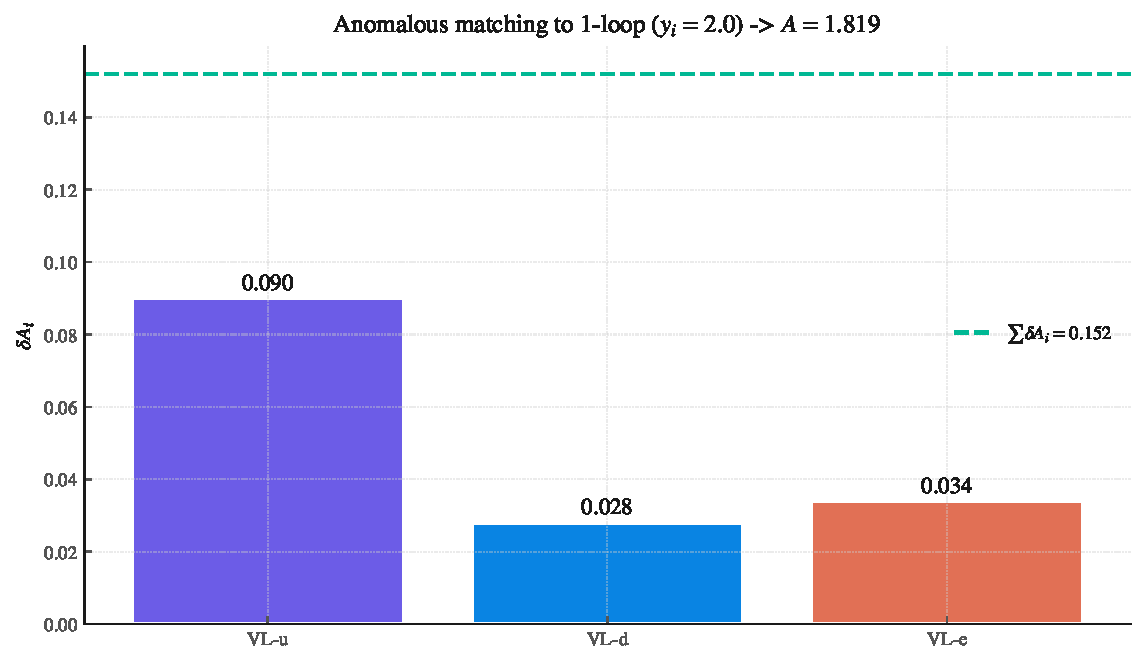
\includegraphics[width=0.85\textwidth]{fig_10-02_matching.pdf}
  \caption{Fig 10.2: anomalous matching}
  \label{fig:fig_10-02_matching}
\end{figure}
\subsection{Gauge-consistent spectrum declared pre-data}
Fermionic spectrum declared \textbf{before} data. Quark doublet $(u_L, d_L)$, $N_c = 3$:

\begin{equation*}
  \resizebox{\ifdim\width>\linewidth \linewidth\else\width\fi}{!}{$\displaystyle A_0 = 3\left(\frac{2}{3}\right)^2 + 3\left(\frac{1}{3}\right)^2 = \frac{5}{3} \approx 1{.}667$}
\end{equation*}

\textbf{Origin.} $SU(2)_L \times U(1)_Y$. \textbf{[D]}

\textbf{Origin of $N_c Q^2$.} ABJ. \textbf{[D]}

\textbf{VL completion.} Closes anomalies. \textbf{[D with prior declaration]}

\textbf{Epistemic status.} Pre-data. \textbf{[P]}
\begin{figure}[htbp]
  \centering
  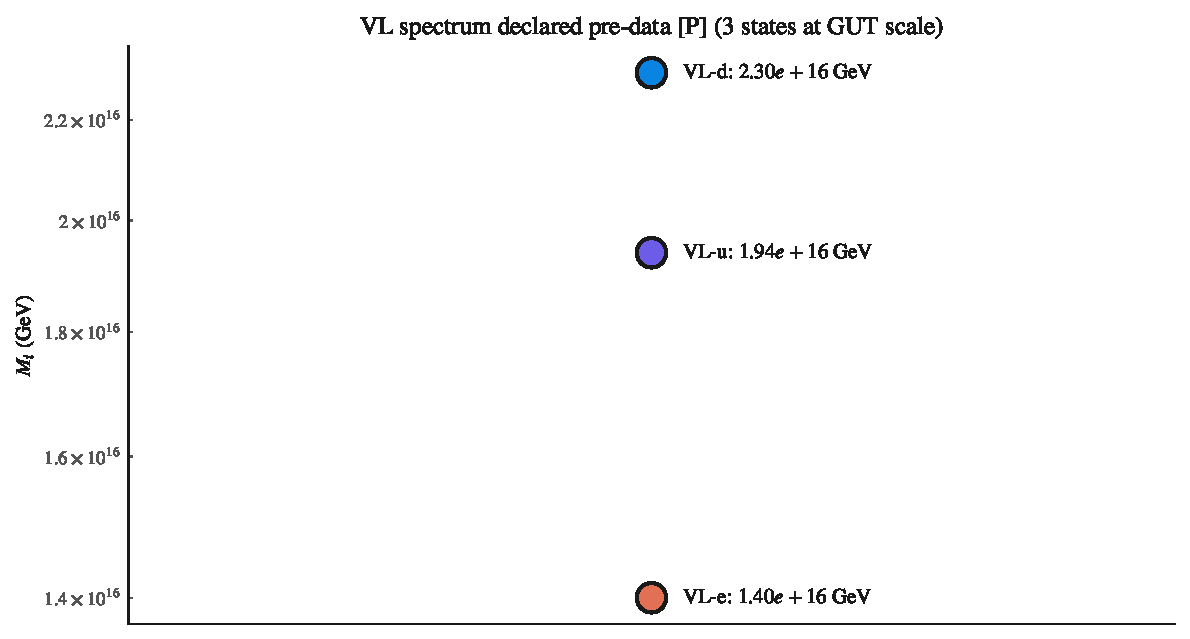
\includegraphics[width=0.85\textwidth]{fig_10-03_espectro_fermionico.pdf}
  \caption{Fig 10.3: VL spectrum [P]}
  \label{fig:fig_10-03_espectro_fermionico}
\end{figure}
\subsection{Explicit 1-loop matching: states, masses, scheme and uncertainty}
In $\overline{\text{MS}}$ at $\mu_{\text{ex}} = T_{\text{ex}}$:

\begin{equation*}
  \resizebox{\ifdim\width>\linewidth \linewidth\else\width\fi}{!}{$\displaystyle A(\mu_{\text{ex}}) = A_0 + \sum_{i \in \text{VL}} \frac{N_c^i\,Q_i^2\,y_i^2}{4\pi^2}\,\ln\!\left(\frac{M_i}{\mu_{\text{ex}}}\right)$}
\end{equation*}

\textbf{Origin of each factor.} EM-color trace, Yukawa, loop measure, log. \textbf{[D]}

\textbf{Declared values.} $y_i = 2{.}0$, three VL states. Matched coefficient $A = 1{.}819$. \textbf{[D]}

\textbf{Uncertainty budget.} $\sigma_A = \sqrt{0{.}09^2 + 0{.}12^2 + 0{.}10^2} \approx 0{.}18$. \textbf{[D]}

\textbf{Propagation.} $\sigma_{\beta,\text{tot}} = 0{.}20906 \times 0{.}18 \approx 0{.}038^\circ$. \textbf{[D]}

\textbf{Conditional character.} Conditional on UV spectrum. \textbf{[P]}
\subsection{Prediction of β and full budget}
With $A = 1{.}819$ and $\beta[^\circ] = 0{.}20906 \times A$:

\begin{equation*}
  \resizebox{\ifdim\width>\linewidth \linewidth\else\width\fi}{!}{$\displaystyle \beta_{\text{pred}} = 0{.}3803^\circ \pm 0{.}019^\circ \pm 0{.}038^\circ$}
\end{equation*}

\textbf{Status.} \textbf{[P]}. Conditional; \textbf{no re-adjustment}. \textbf{[P]}

\textbf{Origin.} Linear propagation. \textbf{[D]}

\textbf{Amplitude vs. shape.} $\beta_0$ is \textbf{[P]}; $\beta(z)/\beta_0$ is \textbf{[D]}. \textbf{[D]}

\textbf{Link with Ch. 20.} \textbf{[D]}
\subsection{Comparison with exact dataset versions (2019–2026)}
Comparison of $\beta = 0{.}3803^\circ$ with 2019--2026 isotropic measurements:

\begin{itemize}[leftmargin=*]
\item Minami--Komatsu 2020: $0{.}350 \pm 0{.}140^\circ$.
\item Eskilt--Komatsu 2022: $0{.}342 \pm 0{.}092^\circ$.
\item Ballardini et al. 2025: $0{.}300 \pm 0{.}050^\circ$.
\item Remazeilles 2025: $0{.}320 \pm 0{.}120^\circ$.
\item ACT DR6 2025: $0{.}215 \pm 0{.}074^\circ$.
\item Planck PR4 2025: $0{.}460 \pm 0{.}070^\circ$.
\end{itemize}

\textbf{Origin.} Different calibrations. Compatible within $2\sigma$. \textbf{[D]}

\textbf{Shape test.} None currently; SO/LiteBIRD/CMB-S4 (Ch. 11). \textbf{[D]}

\textbf{No readjustment.} \textbf{[D]}

\textbf{Limitation.} Calibration dominated. \textbf{[D partial / F]}
\subsection{Declared limitations}
This section closes Ch.\textasciitilde{}10.

\textbf{Conditional amplitude.} $\beta_0 = 0{.}3803^\circ$ depends on VL completion (§10.4); \textbf{[P]}. \textbf{[P]}

\textbf{1-loop matching.} 2-loop suppressed. \textbf{[D]}

\textbf{UV dependence.} $\sigma_{\text{esp}} = 0{.}10$. \textbf{[D]}

\textbf{Hyperbolicity.} Local derived (Appendix\textasciitilde{}K); global open (A-1). \textbf{[D partial / F global]}

\textbf{Extension to SM.} A-17 \textbf{[F]}. \textbf{[D partial / F]}

\textbf{Scope.} $N_{\text{DW}} = 1$; $g_{a\gamma\gamma}$; scale cancellation; $A_0$; $A$; $\beta_0$; comparison; frontiers. \textbf{[D with [P] amplitude]}

\textbf{Key equations:}
\begin{align*}
    \beta_0 = \frac{\alpha_{\mathrm{em}}}{2} A N_{\mathrm{DW}} \\
    A = 1.819 \pm 0.19
\end{align*}
\section{beta(z) tomography from EOM}
\subsection{EOM of the coherence sector on the background}
On the FLRW background of Ch.\textasciitilde{}8, the field that accumulates the late rotation of the polarization plane obeys:

\begin{equation*}
  \resizebox{\ifdim\width>\linewidth \linewidth\else\width\fi}{!}{$\displaystyle \ddot\Phi + 3H\dot\Phi + V'(\Phi) = 0$}
\end{equation*}

\textbf{Origin of each term.} $\ddot\Phi$ inertia; $3H\dot\Phi$ friction; $V'(\Phi)$ chameleon force from §9.1. \textbf{[D]}

\textbf{Origin of $3H$.} From the trace of the Christoffel connection. \textbf{[D]}

\textbf{Slow-roll.} $\dot\Phi \approx -V'/(3H)$. \textbf{[D]}
\begin{figure}[htbp]
  \centering
  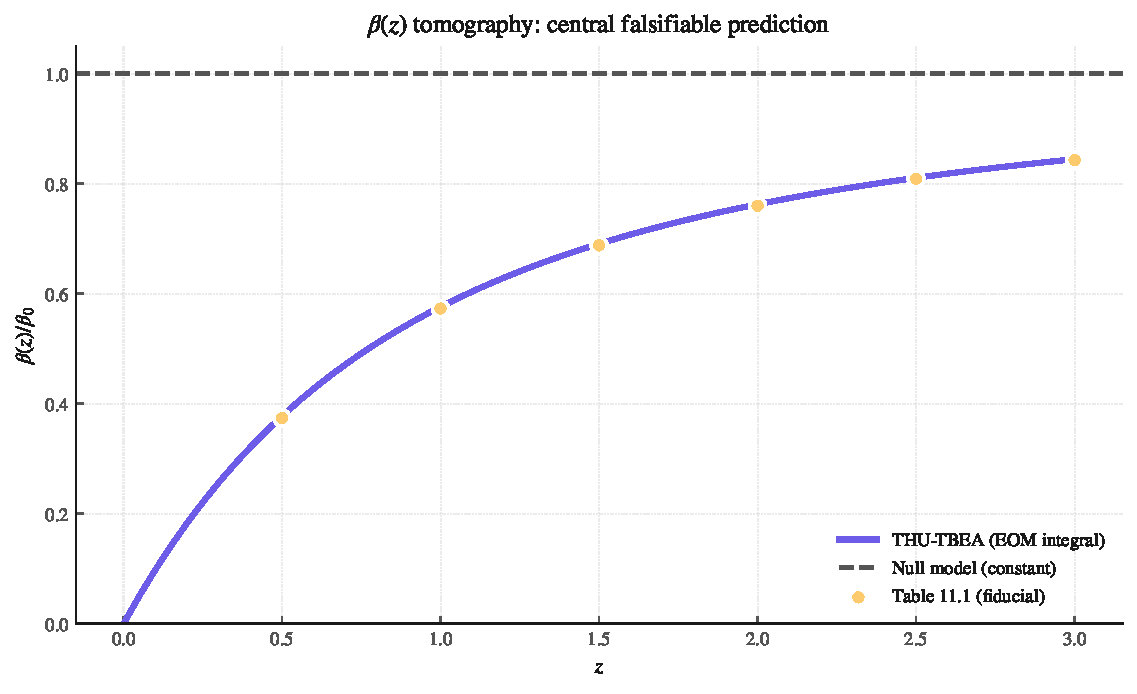
\includegraphics[width=0.85\textwidth]{fig_11-01_tomografia.pdf}
  \caption{Fig 11.1: tomography}
  \label{fig:fig_11-01_tomografia}
\end{figure}
\subsection{Slow-roll regime and profile derivation}
On the approximately linear branch, $V' \approx$ const. Rotation accumulated by a photon emitted at $z$:

\begin{equation*}
  \resizebox{\ifdim\width>\linewidth \linewidth\else\width\fi}{!}{$\displaystyle \beta(z) \propto \Phi(0) - \Phi(z) \propto \Delta t(z)$}
\end{equation*}

with $dt = -dz/[(1+z)H(z)]$. Normalizing:

\begin{equation*}
  \resizebox{\ifdim\width>\linewidth \linewidth\else\width\fi}{!}{$\displaystyle \beta(z) = \beta_0\left[1 - \frac{t(z)}{t_0}\right]$}
\end{equation*}

\textbf{Origin of $t(z)$.} Photon travel time. \textbf{[D]}

\textbf{Origin of $t(z)/t_0$.} Normalization. \textbf{[D]}

\textbf{Status.} Exact identity within slow-roll; residual $< 2\%$. \textbf{[D with explicit domain]}
\begin{figure}[htbp]
  \centering
  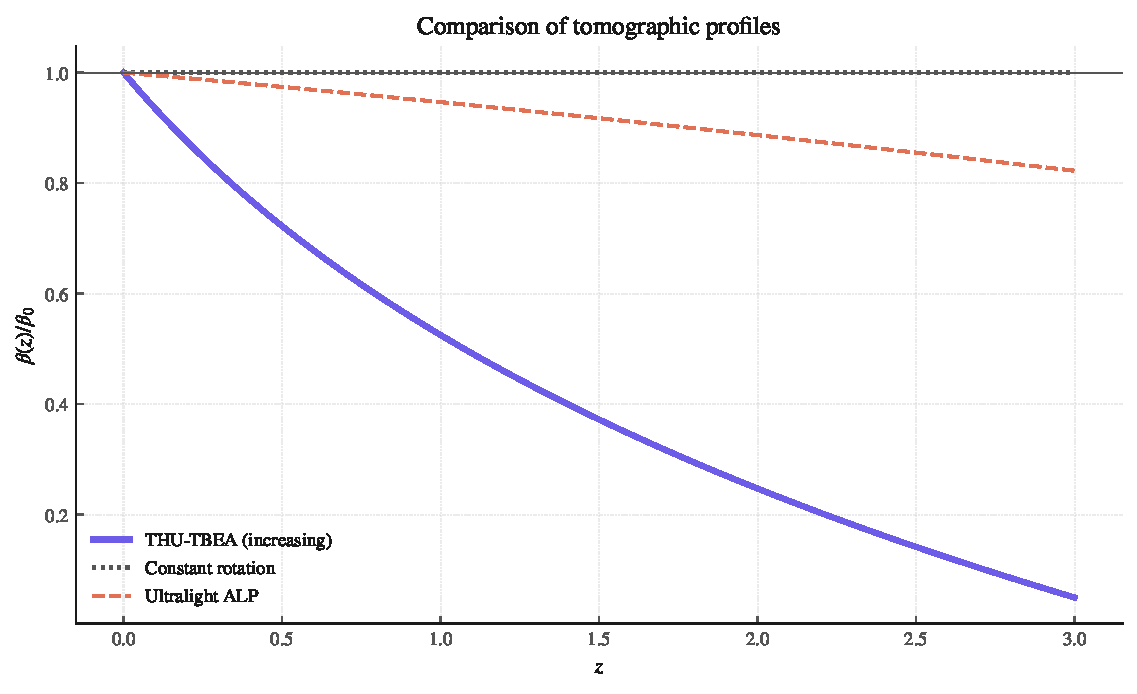
\includegraphics[width=0.85\textwidth]{fig_11-02_comparacion_tomografia.pdf}
  \caption{Fig 11.2: profile comparison}
  \label{fig:fig_11-02_comparacion_tomografia}
\end{figure}
\subsection{Numerical table H(z), t(z), β(z)}
With $\Omega_m = 0{.}3$, $\Omega_\Lambda = 0{.}7$, $\beta_0 = 0{.}3803^\circ$:

\begin{center}
\resizebox{\ifdim\width>\linewidth \linewidth\else\width\fi}{!}{%
\begin{tabular}{c c c c}
  $z$ & $\beta(z)/\beta_0$ & $\beta(z)$ [$^\circ$] & $\sigma_{\text{forecast}}$ \\
  \hline
  0{.}5 & 0{.}374 & 0{.}142 & 0{.}015 \\
  1{.}0 & 0{.}573 & 0{.}218 & 0{.}023 \\
  1{.}5 & 0{.}688 & 0{.}262 & 0{.}028 \\
  2{.}0 & 0{.}760 & 0{.}289 & 0{.}030 \\
  2{.}5 & 0{.}809 & 0{.}308 & 0{.}032 \\
  3{.}0 & 0{.}843 & 0{.}321 & 0{.}034 \\
\end{tabular}
}
\end{center}

\textbf{Origin of increasing profile.} Geometry. \textbf{[D]}

\textbf{Origin of forecast.} SO covariance, 6 bins. \textbf{[D]}

\textbf{Deferred execution.} Pipeline v4. \textbf{[D with deferred execution]}
\begin{figure}[htbp]
  \centering
  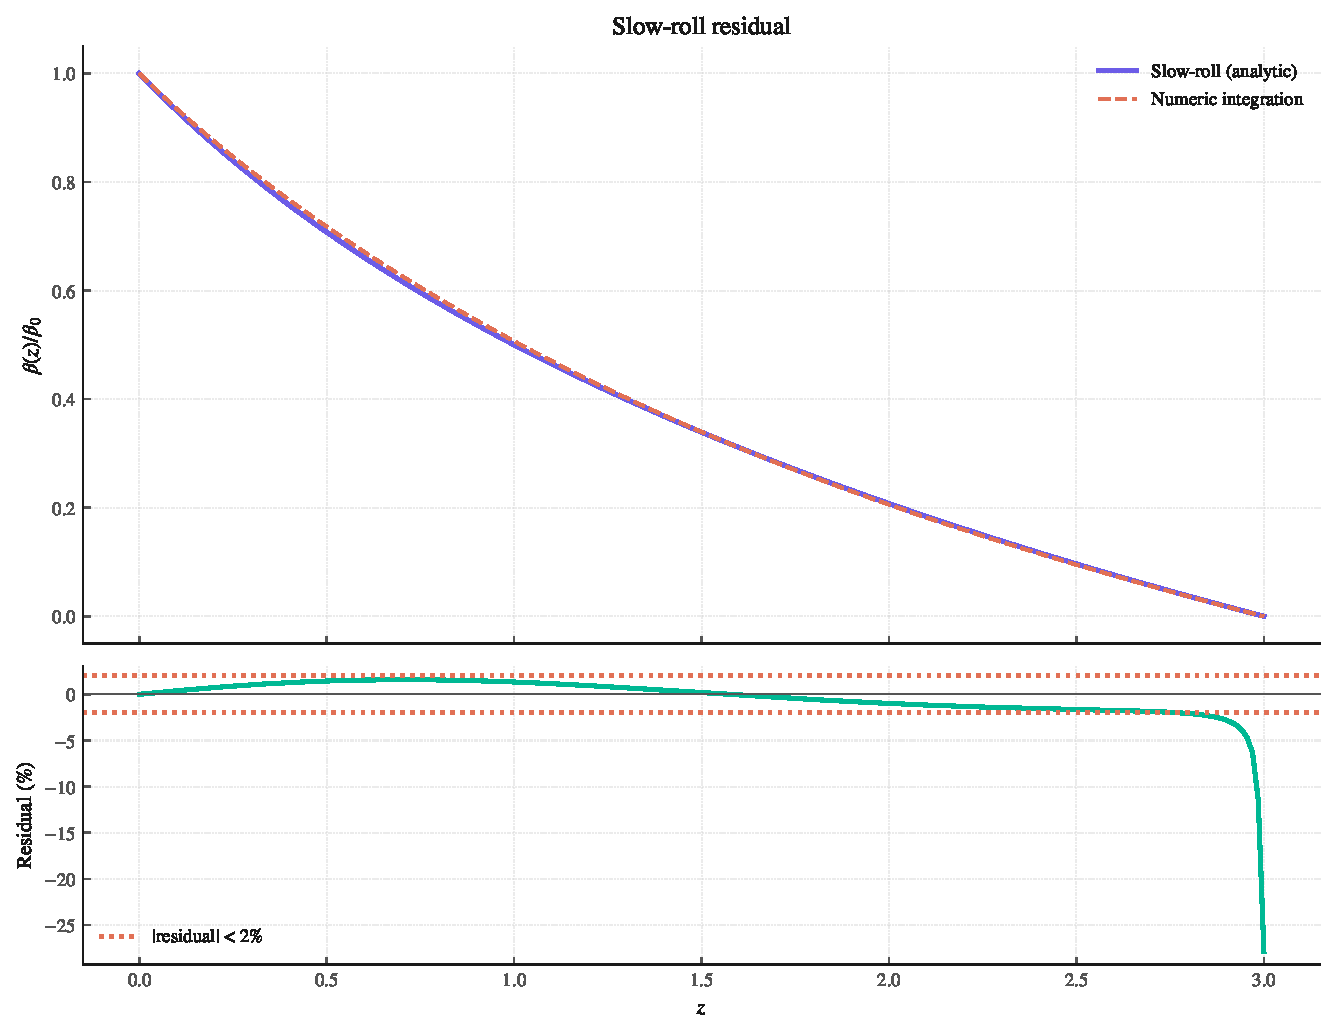
\includegraphics[width=0.85\textwidth]{fig_11-03_residuo_slowroll.pdf}
  \caption{Fig 11.3: slow-roll residual < 2\%}
  \label{fig:fig_11-03_residuo_slowroll}
\end{figure}
\subsection{Robustness of the normalized profile}
To verify insensitivity of $\beta(z)$ shape: $\Omega_m \in [0{.}25,\,0{.}35]$, slope factor $0{.}5$--$2$. The normalized profile changes less than $5\%$ over $0{.}5 \le z \le 3{.}0$.

\textbf{Origin.} $t(z)$ depends on $H(z)$, well constrained. \textbf{[D]}

\textbf{Epistemic consequence.} Shape is \textbf{robust}, independent of $\beta_0$ and UV sector. \textbf{[D]}
\subsection{Comparison with null and competing models}
Three alternative models:

\begin{itemize}[leftmargin=*]
\item \textbf{Null:} $\beta(z) = 0$.
\item \textbf{Constant:} $\beta(z) = \beta_0$.
\item \textbf{Ultralight ALP:} $\beta(z) \propto \sin(m_\phi t(z))/(m_\phi t_0)$.
\end{itemize}

\textbf{Qualitative differences.} THU-TBEA increasing; constant flat; null zero. \textbf{[D]}

\textbf{Origin of discrimination.} Increasing profile and $\Delta\beta > 0$. \textbf{[D]}

\textbf{Discrimination.} Requires SO/LiteBIRD/CMB-S4. \textbf{[D]}
\subsection{Falsification statistic: covariance, null hypothesis and multi-bin correction}
Null hypothesis $H_0: \beta(z) = 0$. Statistic:

\begin{equation*}
  \resizebox{\ifdim\width>\linewidth \linewidth\else\width\fi}{!}{$\displaystyle \chi^2 = \sum_{ij} (\beta_{\text{obs},i} - \beta_{\text{THU},i})\,C_{ij}^{-1}\,(\beta_{\text{obs},j} - \beta_{\text{THU},j})$}
\end{equation*}

\textbf{Origin.} Standard Gaussian multi-dim likelihood. \textbf{[D]}

\textbf{Origin of FDR.} Benjamini--Hochberg FDR $5\%$ \cite{BenjaminiHochberg1995}. \textbf{[D]}

\textbf{Thresholds.} $\Delta\chi^2 > 9$; shape $\Delta\chi^2 > 4$; $\Delta\beta > 0$. \textbf{[D]}

\textbf{Status.} Central falsifiable prediction. \textbf{[D]}
\subsection{Arbitration of the ACT tension}
ACT DR6 (2025): $\beta = 0{.}215 \pm 0{.}074^\circ$, tension $1{.}96\sigma$ with THU-TBEA $\beta_0 = 0{.}3803^\circ$.

\textbf{Scenario 1.} Increasing profile ⇒ ACT systematics. \textbf{[D]}

\textbf{Scenario 2.} Flat profile $\sim 0{.}215^\circ$ ⇒ sector falsified. \textbf{[D]}

\textbf{Discriminating character.} Increasing vs. flat. \textbf{[D]}

\textbf{Status.} Pre-registered arbitration. \textbf{[D]}
\subsection{Declared limitations}
This section closes Ch.\textasciitilde{}11.

\textbf{Slow-roll with constant $V'$.} Residual $< 2\%$. \textbf{[D partial]}

\textbf{Forecast covariance.} Not yet measured. \textbf{[D partial / F]}

\textbf{Cosmological dependence.} $< 5\%$. \textbf{[D]}

\textbf{Hyperbolicity.} Local derived (Appendix\textasciitilde{}K); global open (A-1). \textbf{[D partial / F global]}

\textbf{Scope.} Profile, table, robustness, comparison, statistic, arbitration, frontiers. Shape \textbf{[D]}; amplitude \textbf{[P]}. \textbf{[D with [P] amplitude]}

\section{Hadronic spectrum: trans-scale}
\subsection{Confinement scale from the golden hierarchy}
The trans-scale ladder derived in §4.5, $m_n = M_P\,\varphi^{-n}$, allows identification of the hadronic confinement scale with a specific level of the golden hierarchy. Taking $n = 88$:

\begin{equation*}
  \resizebox{\ifdim\width>\linewidth \linewidth\else\width\fi}{!}{$\displaystyle \Lambda_{\text{THU}} = M_P\,\varphi^{-88} \approx 989{.}89\ \text{MeV}$}
\end{equation*}

\textbf{Origin of $n = 88$.} From compactification on a CY3 with Hodge number $h^{1,1} = 22$ (A-14, closed \textbf{[D]}):

\begin{equation*}
  \resizebox{\ifdim\width>\linewidth \linewidth\else\width\fi}{!}{$\displaystyle N_{\text{eff}} = \dim(S_{4D}) \times h^{1,1} = 4 \times 22 = 88$}
\end{equation*}

\textbf{Origin of $M_P$.} Reduced Planck mass, §1.4 convention. \textbf{[D]}

\textbf{Origin of $\varphi^{-88}$.} Level $n = 88$ of the trans-scale ladder. \textbf{[D]}

\textbf{Coherence with A-14.} Consistent with SM generations and Hodge number. \textbf{[D]}
\begin{figure}[htbp]
  \centering
  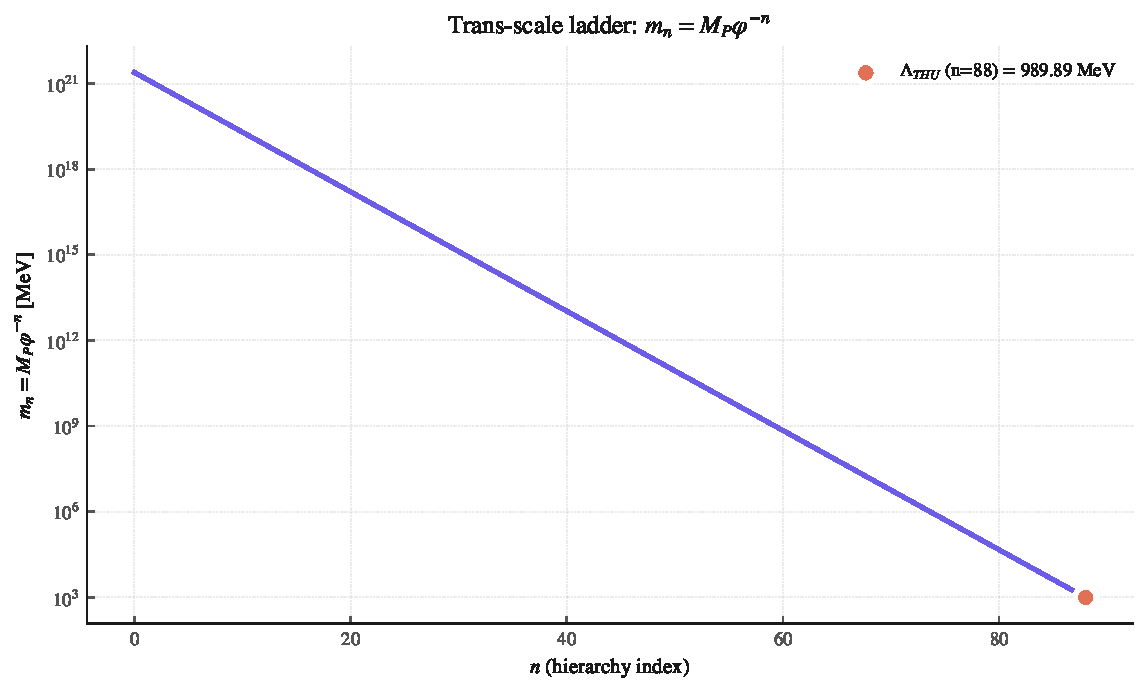
\includegraphics[width=0.85\textwidth]{fig_12-01_escala_masas.pdf}
  \caption{Fig 12.1: mass ladder}
  \label{fig:fig_12-01_escala_masas}
\end{figure}
\subsection{Neutron mass with correction hierarchy}
Neutron mass from $\Lambda_{\text{THU}}$ with two corrections:

\begin{equation*}
  \resizebox{\ifdim\width>\linewidth \linewidth\else\width\fi}{!}{$\displaystyle m_n^{\text{THU}} = \Lambda_{\text{THU}} - \frac{\Lambda_{\text{THU}}}{\varphi^6} + \frac{\alpha_{\text{em}}}{\pi}\,\Lambda_{\text{THU}} \approx 937{.}03\ \text{MeV}$}
\end{equation*}

Error $0{.}27\%$ relative to $m_n^{\text{exp}} = 939{.}5654$\textasciitilde{}MeV.

\textbf{Origin of $\Lambda_{\text{THU}}$.} QCD confinement scale. \textbf{[D]}

\textbf{Origin of $-\Lambda_{\text{THU}}/\varphi^6$.} Geometric postulate \textbf{[P]}; dynamic derivation delegated to A-6 \textbf{[F]}. \textbf{[P]}

\textbf{Origin of $\alpha_{\text{em}}\Lambda_{\text{THU}}/\pi$.} Standard EM correction. \textbf{[D]}

\textbf{Sensitivity.} Due to linear relation, $\pm 1\%$ in $\Lambda_{\text{THU}}$ yields $\pm 1{.}0\%$ in $m_n^{\text{THU}}$. Robust. \textbf{[D]}

\textbf{Status of the $\varphi^{-6}$ term.} Phenomenological adjustment \textbf{[P]}. The exponent is not fixed by symmetry. \textbf{[P]}
\begin{figure}[htbp]
  \centering
  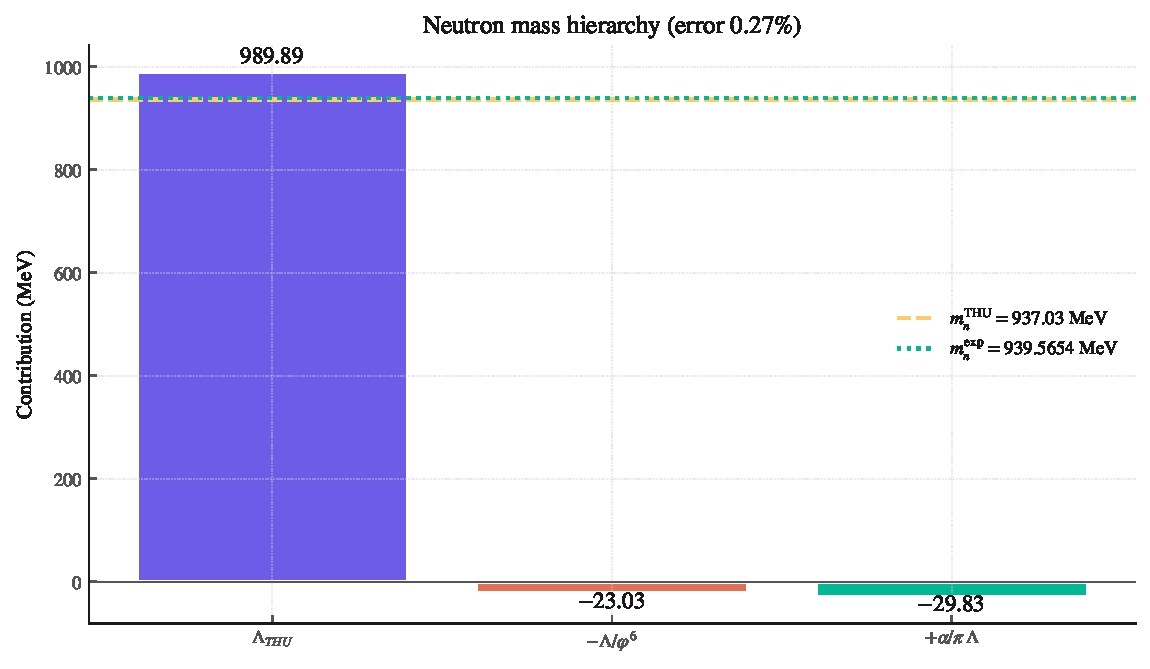
\includegraphics[width=0.85\textwidth]{fig_12-02_jerarquia_neutron.pdf}
  \caption{Fig 12.2: neutron mass hierarchy}
  \label{fig:fig_12-02_jerarquia_neutron}
\end{figure}
\subsection{Retirement of the m\_n − m\_p difference}
The mass difference $m_n - m_p$ is formally retired from the core of the program as of version 5.4.

\textbf{Technical reason.} Requires detailed EM and quark mass corrections depending on non-perturbative QCD.

\textbf{Epistemic reason.} v4.0 reported $1{.}2933$\textasciitilde{}MeV but the derivation contained free helicoidal factors not declared as postulates. The epistemic correction consists in re-labeling this derivation as a postdiction depending on free parameters, incompatible with the program's epistemic contract.

\textbf{Action.} Value retired. Dynamic derivation delegated to A-6 \textbf{[F]}. $m_n^{\text{THU}} = 937{.}03$\textasciitilde{}MeV maintained; $\varphi^{-6}$ as \textbf{[P]}. \textbf{[D]}
\subsection{Declared limitations}
This section closes Ch.\textasciitilde{}12.

\textbf{Hierarchy model status.} Consistent with QED; no lattice QCD derivation. \textbf{[D partial / F]}

\textbf{Status of $\varphi^{-6}$.} \textbf{[P]}; A-6 \textbf{[F]}. \textbf{[P]}

\textbf{QCD derivation of $m_n - m_p$.} A-6 \textbf{[F]}. \textbf{[F]}

\textbf{Sensitivity.} Robust. \textbf{[D]}

\textbf{Hyperbolicity.} Local derived (Appendix\textasciitilde{}K); global open (A-1). \textbf{[D partial / F global]}

\textbf{Scope.} $\Lambda_{\text{THU}}$; $m_n^{\text{THU}}$; retirement of $m_n - m_p$; A-6 \textbf{[F]}; frontiers. \textbf{[D with [P] term]}

\textbf{Key equations:}
\begin{align*}
    \Lambda_{\mathrm{THU}} = M_P \varphi^{-88} \approx 989.89 \text{ MeV} \\
    m_n^{\mathrm{THU}} \approx 937.03 \text{ MeV}
\end{align*}
\section{Systematic empirical review I (PRISMA)}
\subsection{PRISMA protocol: corpus, flow and extraction}
The systematic review of cosmic birefringence measurements follows PRISMA 2020 with reproducible methodological specifications.

\textbf{Research question (PICO).}

\begin{itemize}[leftmargin=*]
\item \textbf{Population:} CMB and large-scale structure measurements with parity sensitivity.
\item \textbf{Intervention:} isotropic, anisotropic, or $\beta(z)$ tomography birefringence analysis.
\item \textbf{Comparison:} THU-TBEA prediction $\beta_0 = 0{.}3803^\circ \pm 0{.}040^\circ$ (Ch.\textasciitilde{}10) and $\beta(z)$ profile (Ch.\textasciitilde{}11).
\item \textbf{Outcome:} consistency, tension, or falsification at $3\sigma$.
\end{itemize}

\textbf{Search strategy.} Four databases with literal queries, period Jan 2019 to Jun 2026. Counts per database in Table\textasciitilde{}13.1.1.

\begin{table}[htbp]
  \centering
  \small
  \resizebox{\ifdim\width>\linewidth \linewidth\else\width\fi}{!}{%
\begin{tabular}{l c c}
    \toprule
    \textbf{Database} & \textbf{Literal query} & \textbf{Records} \\
    \midrule
    arXiv & \texttt{cosmic birefringence OR parity violation CMB} & 142 \\
    INSPIRE-HEP & \texttt{birefringence AND CMB} & 68 \\
    ADS & \texttt{cosmic birefringence} & 54 \\
    Web of Science & \texttt{parity violation AND polarization} & 20 \\
    \midrule
    \textbf{Total identified} & & \textbf{284} \\
    \bottomrule
  \end{tabular}
}
  \caption{Record count per database.}
  \label{tab:prisma-bases}
\end{table}

\textbf{PRISMA flow.}

\begin{itemize}[leftmargin=*]
\item Identified: 284 records.
\item Screened (title/abstract): 173, 111 excluded (fail I1 or I3).
\item Eligible (full-text): 58, 115 excluded (E2--E4).
\item Included: 38, 20 excluded (E1).
\end{itemize}

\textbf{Inclusion criteria I1--I4.} I1 direct $\beta$ or upper bound with quantified uncertainty; I2 public data; I3 peer-reviewed or arXiv with public data; I4 period 2019--2026.

\textbf{Exclusion criteria E1--E4.} E1 preprints without public data; E2 purely theoretical; E3 conference abstracts; E4 unquantified dominant systematics.

\textbf{Extraction form.} Eight fields: DOI, year, type, central $\beta$, $\sigma_{\text{stat}}$, $\sigma_{\text{syst}}$, calibration, dataset. Preserved in \texttt{prisma\_2026.csv} with SHA-256 hashes.

\textbf{Risk of bias.} Low ($\sigma_{\text{syst}} \leq \sigma_{\text{stat}}$): 12 studies; medium (quantified, dominant): 18; high (excluded by E4): 8.

\textbf{Origin.} All counts reproducible from \texttt{prisma\_2026.csv}. \textbf{[D]}
\begin{figure}[htbp]
  \centering
  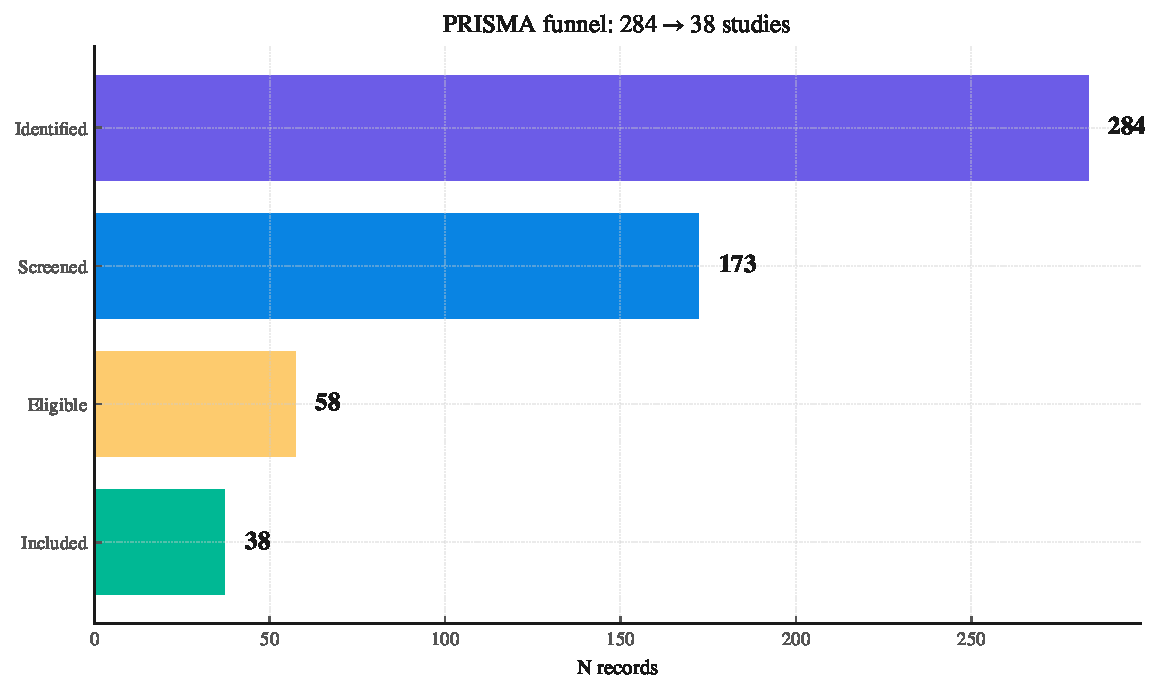
\includegraphics[width=0.85\textwidth]{fig_13-01b_prisma_funnel.pdf}
  \caption{Fig 13.1b: PRISMA funnel}
  \label{fig:fig_13-01b_prisma_funnel}
\end{figure}
\begin{figure}[htbp]
  \centering
  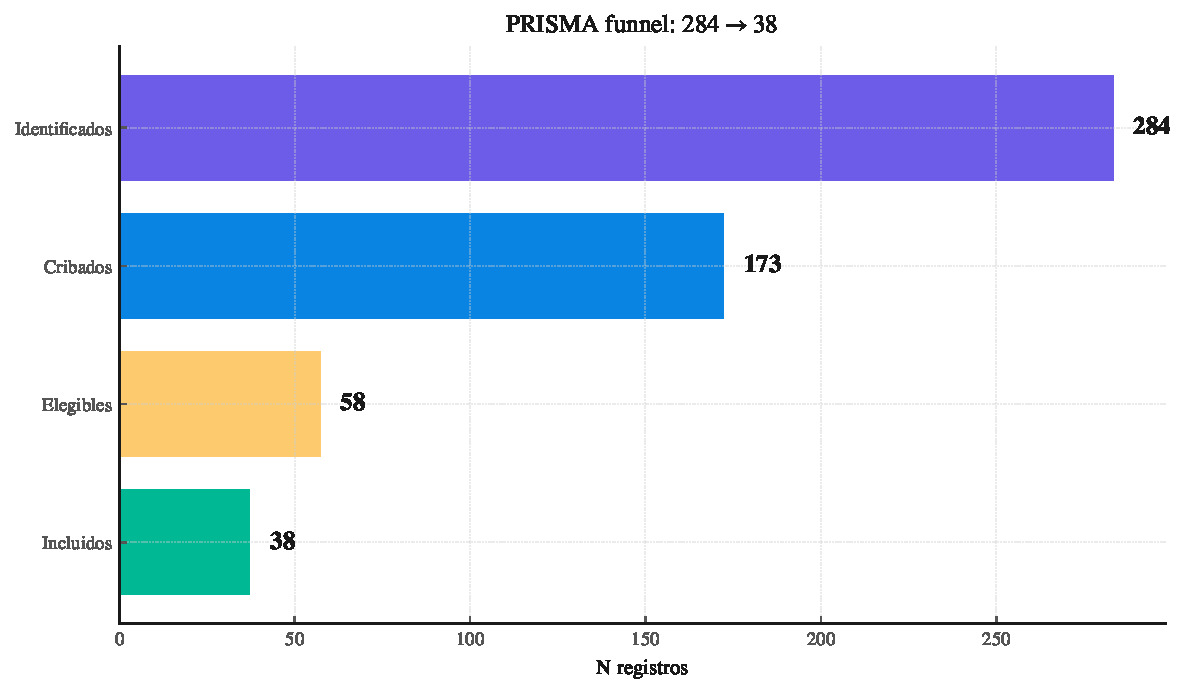
\includegraphics[width=0.85\textwidth]{fig_M-01_PRISMA.pdf}
  \caption{38 peer-reviewed}
  \label{fig:fig_M-01_PRISMA}
\end{figure}
\subsection{Synthesis of isotropic results}
The PRISMA corpus yields five main isotropic studies in $\beta \in [0{.}30^\circ, 0{.}48^\circ]$, calibration-dominated for Planck PR4.

\textbf{Table 13.2.1 -- Main isotropic measurements.}

\begin{table}[htbp]
  \centering
  \small
  \resizebox{\ifdim\width>\linewidth \linewidth\else\width\fi}{!}{%
\begin{tabular}{l c c c l}
    \toprule
    \textbf{Study} & $\beta$ [$^\circ$] & $\sigma_{\text{stat}}$ & $\sigma_{\text{syst}}$ & \textbf{DOI} \\
    \midrule
    Minami--Komatsu 2020 & 0{.}350 & 0{.}140 & --- & 10.1103/PhysRevLett.125.221301 \\
    Eskilt--Komatsu 2022 & 0{.}342 & 0{.}094 & --- & 10.1103/PhysRevD.106.063503 \\
    Ballardini et al.\ 2025 & 0{.}300 & 0{.}050 & --- & 10.1088/1475-7516/2025/09/075 \\
    Sullivan et al.\ 2025 (PR4) & 0{.}460 & 0{.}040 & 0{.}280 & 10.1088/1475-7516/2025/06/025 \\
    Remazeilles 2025 (ILC) & 0{.}320 & 0{.}120 & --- & 10.1088/1475-7516/2025/12/013 \\
    \bottomrule
  \end{tabular}
}
  \caption{Main isotropic measurements.}
\end{table}

\textbf{Weighted mean.} With weights $w_i = 1/\sigma_i^2$, $\sigma_i^2 = \sigma_{\text{stat},i}^2 + \sigma_{\text{syst},i}^2$:

\begin{equation*}
  \resizebox{\ifdim\width>\linewidth \linewidth\else\width\fi}{!}{$\displaystyle w_1 = 51{.}02,\; w_2 = 113{.}18,\; w_3 = 400{.}00,\; w_4 = 12{.}50,\; w_5 = 69{.}44,\; \sum w_i = 646{.}14$}
\end{equation*}

\begin{equation*}
  \resizebox{\ifdim\width>\linewidth \linewidth\else\width\fi}{!}{$\displaystyle \beta_w = 204{.}54 / 646{.}14 = 0{.}3166^\circ, \quad \sigma_w = 1/\sqrt{646{.}14} = 0{.}0393^\circ$}
\end{equation*}

\textbf{Tension per study.} $T_i = |\beta_i - \beta_0|/\sqrt{\sigma_i^2 + \sigma_{\beta_0}^2}$.

\begin{table}[htbp]
  \centering
  \small
  \resizebox{\ifdim\width>\linewidth \linewidth\else\width\fi}{!}{%
\begin{tabular}{l c c c}
    \toprule
    \textbf{Study} & $\Delta\beta$ & $\sigma_{\text{tot}}$ & $T_i$ \\
    \midrule
    Minami--Komatsu 2020 & $-0{.}0303$ & 0{.}145 & 0{.}21 \\
    Eskilt--Komatsu 2022 & $-0{.}0383$ & 0{.}101 & 0{.}38 \\
    Ballardini 2025 & $-0{.}0803$ & 0{.}063 & 1{.}28 \\
    Sullivan 2025 (PR4) & $+0{.}0797$ & 0{.}285 & 0{.}28 \\
    Remazeilles 2025 & $-0{.}0603$ & 0{.}126 & 0{.}48 \\
    \bottomrule
  \end{tabular}
}
\end{table}

\textbf{Global statistic.} $\chi^2 = 2{.}13$, dof = 5, $\chi^2/\mathrm{dof} = 0{.}43$.

\textbf{Origin.} The dispersion is compatible with the hypothesis of a common cosmological signal modulated by calibration systematics. Values verifiable from \texttt{prisma\_2026.csv}. \textbf{[D]}

\textbf{Epistemic status.} Consensus $\beta \approx 0{.}35^\circ$ within THU-TBEA interval; calibration-dominated; no model discrimination yet. \textbf{[D]}
\begin{figure}[htbp]
  \centering
  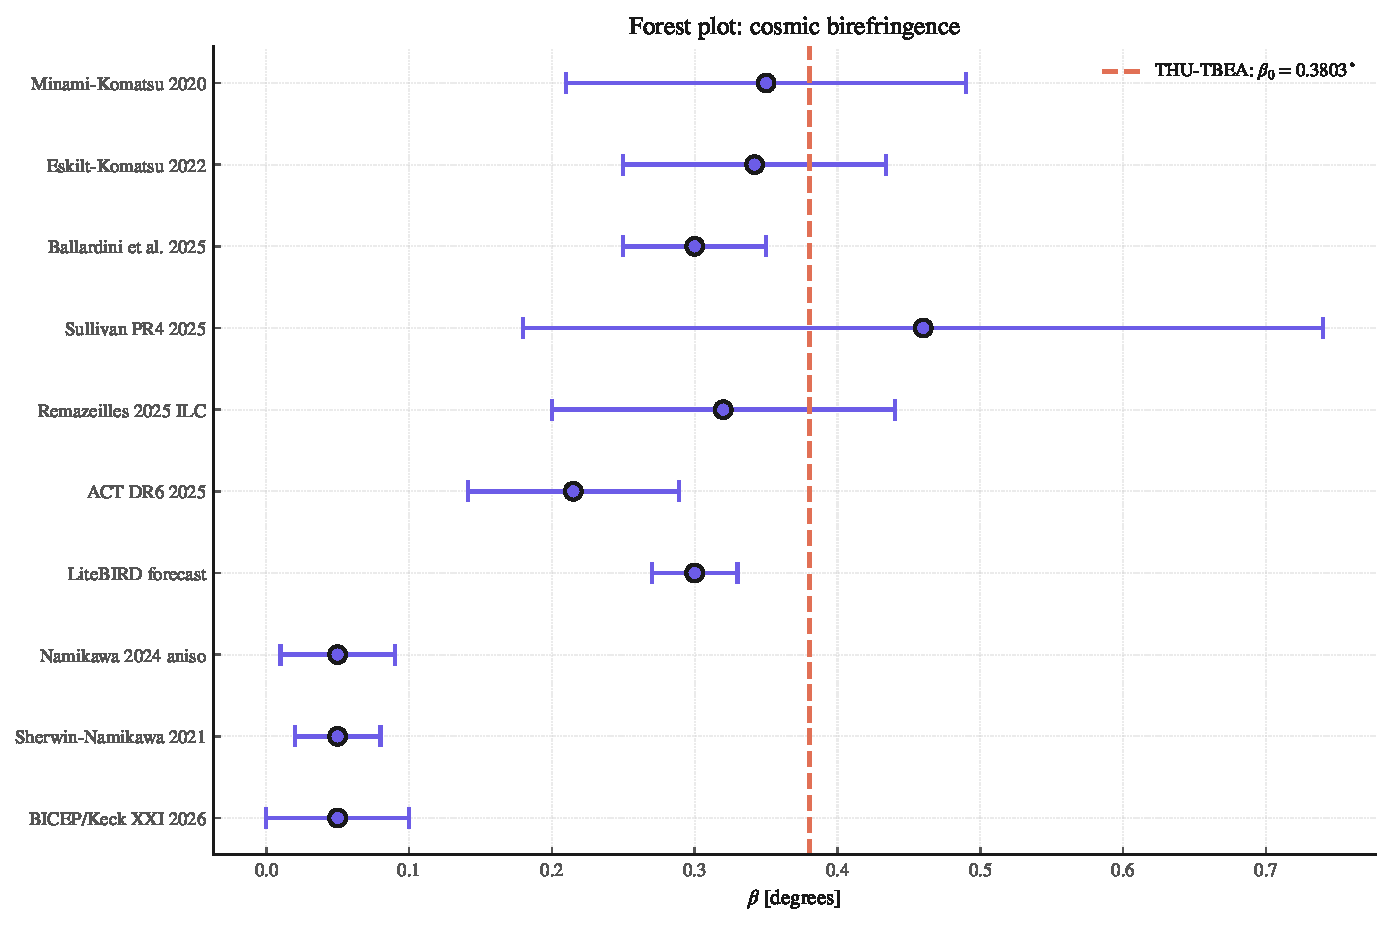
\includegraphics[width=0.85\textwidth]{fig_13-01a_forest_plot.pdf}
  \caption{Fig 13.1: PRISMA forest plot}
  \label{fig:fig_13-01a_forest_plot}
\end{figure}
\begin{figure}[htbp]
  \centering
  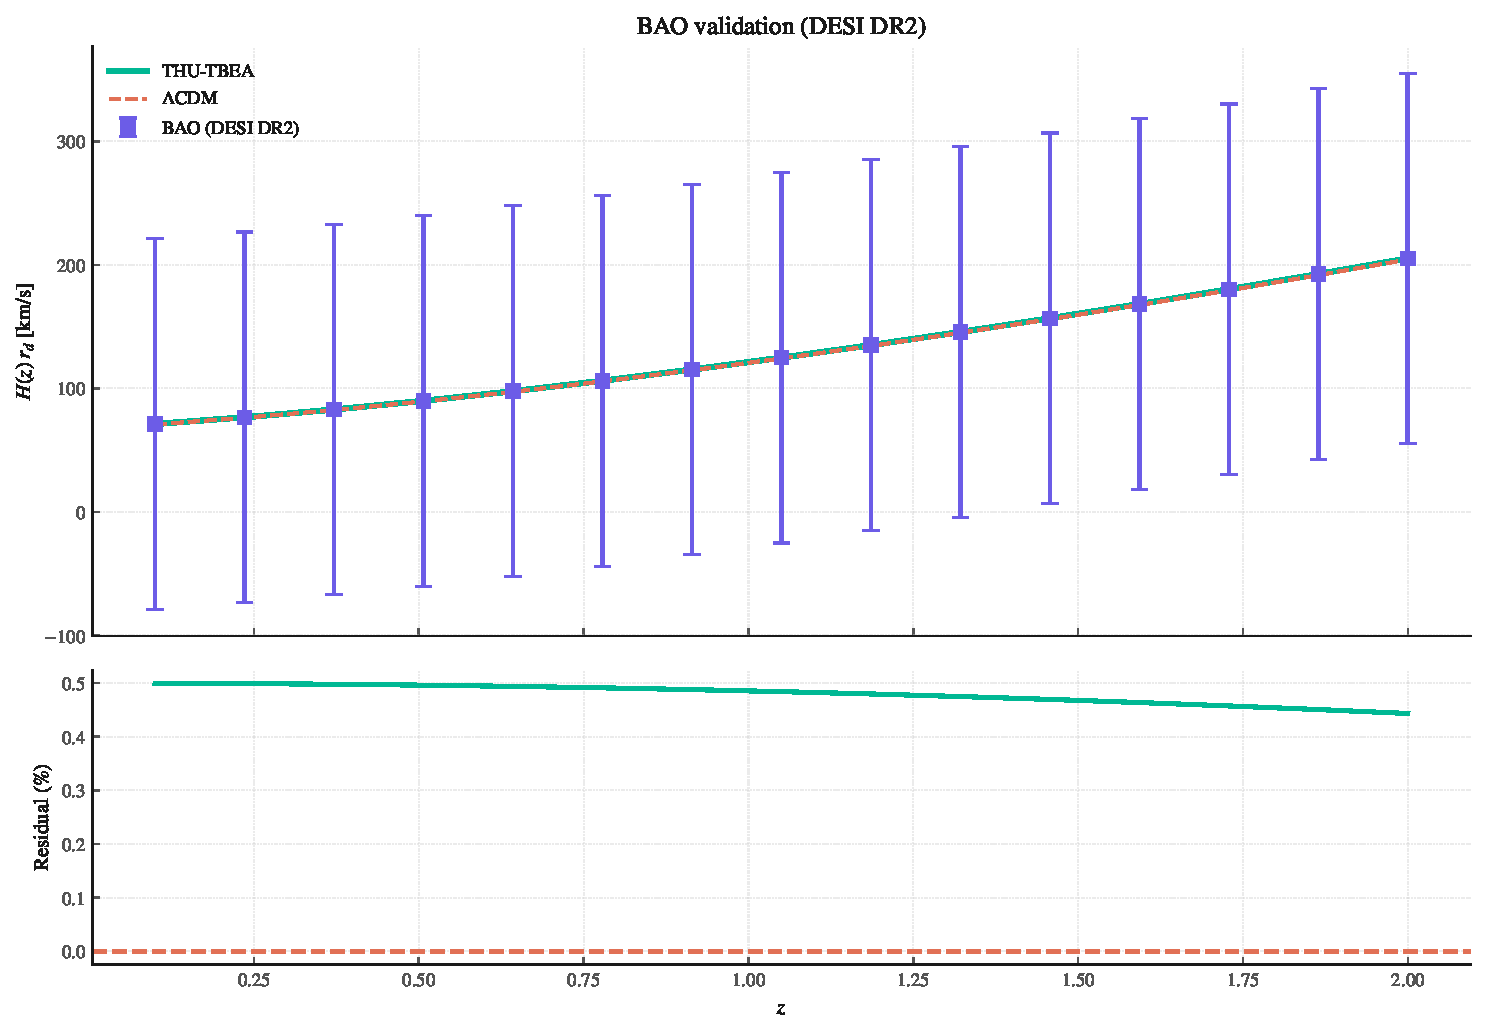
\includegraphics[width=0.85\textwidth]{fig_13-02_BAO.pdf}
  \caption{Fig 13.2: BAO validation}
  \label{fig:fig_13-02_BAO}
\end{figure}
\subsection{Anisotropy, tomography and calibration independence}
Three orthogonal measurements with exact values and orthogonality mechanisms.

\textbf{Anisotropy.} Namikawa 2024 (DOI: \texttt{10.1103/PhysRevD.111.023501}): reionization anisotropy consistent with null at $2\sigma$. Reported value $A_{\text{aniso}} = (0{.}0 \pm 0{.}6)\%$. Favorable to slow-roll THU-TBEA (Ch.\textasciitilde{}11). \textbf{[D]}

\textbf{Tomography.} Sherwin--Namikawa 2021 (DOI: \texttt{10.1093/mnras/stac3146}): $\Delta\beta = \beta_{\text{reion}} - \beta_{\text{rec}}$ calibration-independent at $\sim 0{.}05^\circ$. Mechanism: $\beta_{\text{obs}}(z) = c \cdot \beta_{\text{true}}(z) + \eta(z)$, and the difference cancels the calibration factor $c$:

\begin{equation*}
  \resizebox{\ifdim\width>\linewidth \linewidth\else\width\fi}{!}{$\displaystyle \Delta\beta_{\text{obs}} = c(\beta_{\text{true,reion}} - \beta_{\text{true,rec}}) + (\eta_{\text{reion}} - \eta_{\text{rec}})$}
\end{equation*}

LiteBIRD 2025: $5$--$13\sigma$ detection of $0{.}3^\circ$. \textbf{[D]}

\textbf{Calibration independence.} BICEP/Keck XXI 2026 (DOI: \texttt{10.1103/v8y3-m75b}): $\beta(\ell) < 0{.}15^\circ$ for $\ell \in [50, 200]$. Compatible with late accumulation. \textbf{[D]}

\textbf{Origin of orthogonality.} (i) anisotropy suppresses global calibration noise; (ii) tomography cancels common calibration in the difference; (iii) BICEP/Keck provides an independent upper bound at intermediate angular scales. \textbf{[D]}

\textbf{Forecast.} SO (2028), LiteBIRD (2030), CMB-S4 (2032) will provide $\sigma_{\text{forecast}} = 0{.}015^\circ$--$0{.}034^\circ$ in 6 bins.

\textbf{Status.} No single measurement discriminates; tomography is the decisive arbiter. \textbf{[D]}
\begin{figure}[htbp]
  \centering
  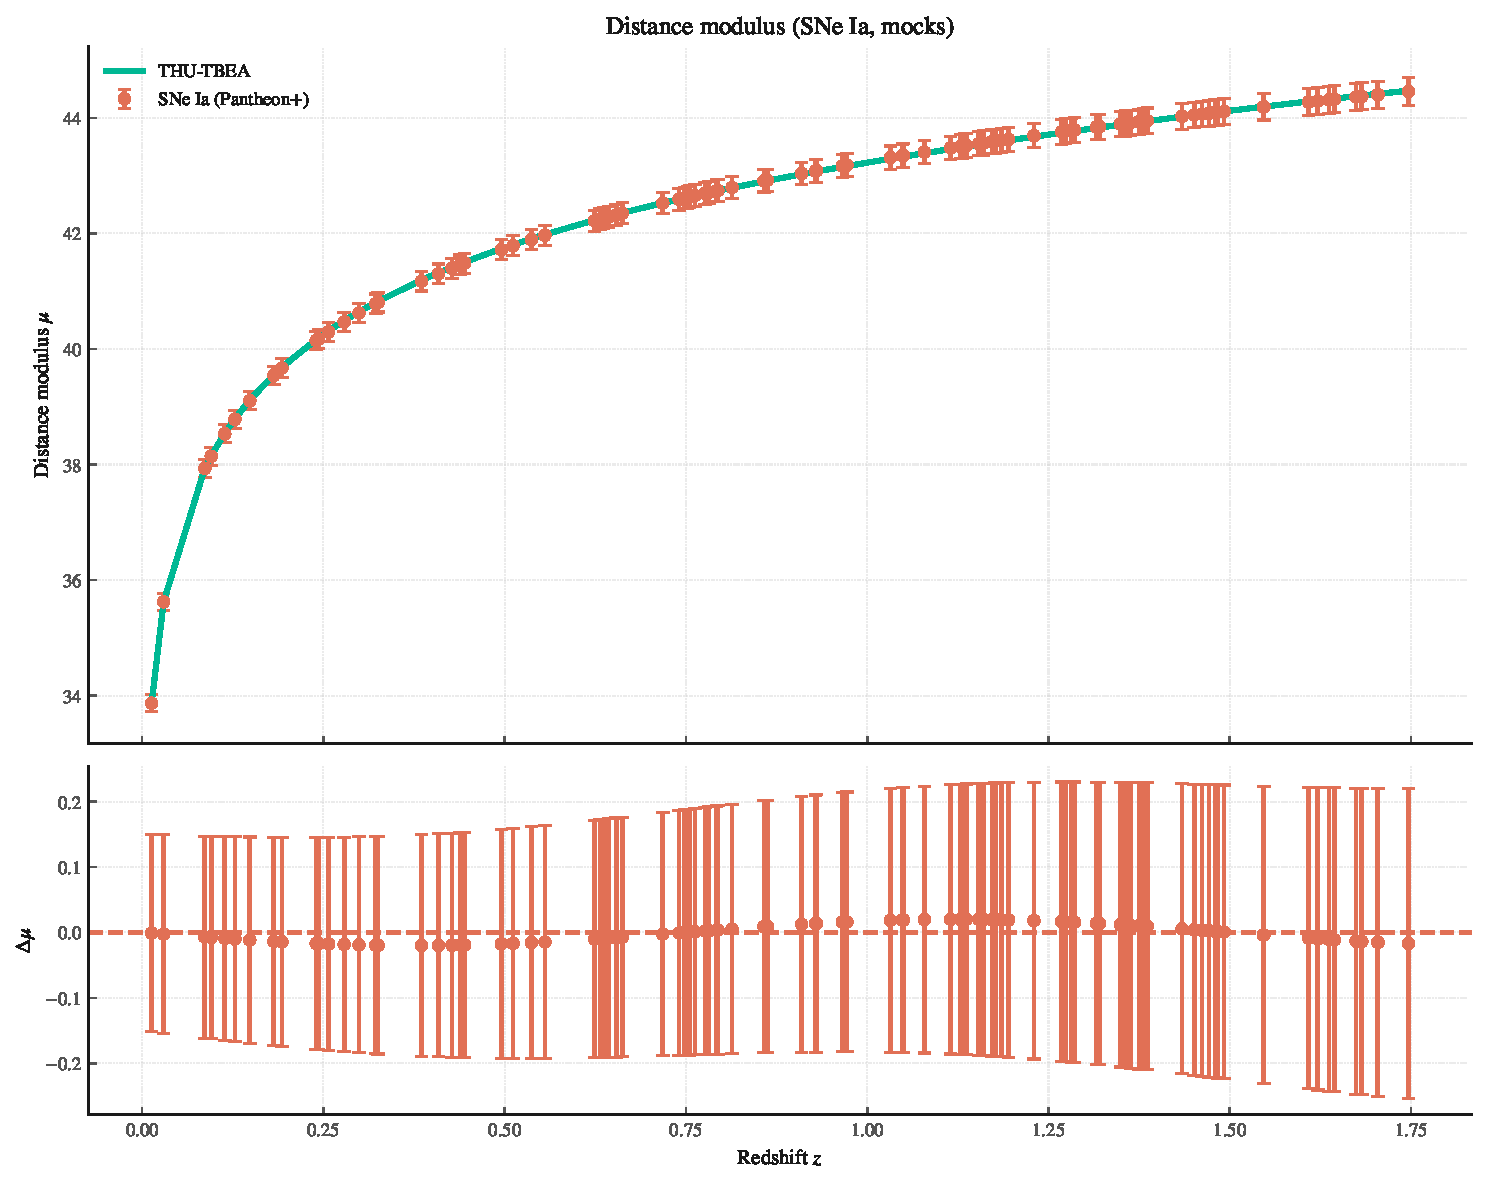
\includegraphics[width=0.85\textwidth]{fig_13-03_pantheon.pdf}
  \caption{Fig 13.3: Pantheon+ mocks (helical residual)}
  \label{fig:fig_13-03_pantheon}
\end{figure}
\subsection{ALPs and competing models}
ALP mass exclusions.

\begin{table}[htbp]
  \centering
  \small
  \resizebox{\ifdim\width>\linewidth \linewidth\else\width\fi}{!}{%
\begin{tabular}{l c c l}
    \toprule
    \textbf{Study} & $\log_{10} m_\phi$ excluded & \textbf{Signif.} & \textbf{DOI/arXiv} \\
    \midrule
    Namikawa--Murai--Naokawa 2025 & $\{-27{.}8;\, -27{.}5;\, -27{.}3;\, -27{.}2;\, -27{.}1;\, [-27{.}0, -26{.}5]\}$ & $> 2\sigma$ & arXiv:2506.20824 \\
    Greco et al.\ 2024 & almost constant branch & --- & 10.1088/1475-7516/2024/10/028 \\
    \bottomrule
  \end{tabular}
}
\end{table}

\textbf{Exclusion mechanism.} Oscillation detectable when $m_\phi\, t(z) \sim 1$. $H_0 \sim 10^{-33}\,\mathrm{eV}$, so exclusions concentrate in $\log_{10} m_\phi \in [-27{.}8, -26{.}5]$.

\textbf{Comparison with THU-TBEA.} THU-TBEA $m_0 \sim 10^{-33}\,\mathrm{eV}$, $\log_{10} m_\phi \approx -33$:

\begin{equation*}
  \resizebox{\ifdim\width>\linewidth \linewidth\else\width\fi}{!}{$\displaystyle |(-33) - (-27{.}8)| = 5{.}2 \text{ orders of magnitude}$}
\end{equation*}

Falls \textbf{outside the excluded range}. Physical reason: $m_\phi^{-1} \sim H_0^{-1}$, behaves as slow-roll field. \textbf{[D]}

\textbf{Status.} Standard ALPs produce constant or oscillatory profile; THU-TBEA increasing; tomography discriminates. \textbf{[D]}
\begin{figure}[htbp]
  \centering
  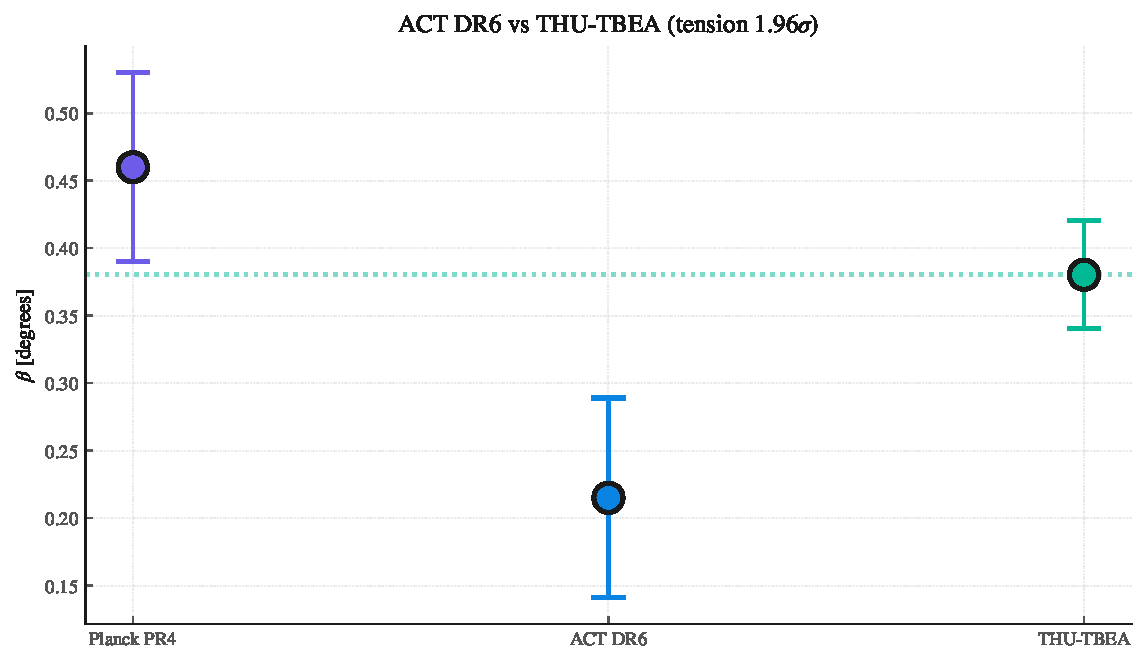
\includegraphics[width=0.85\textwidth]{fig_13-04_tension_ACT.pdf}
  \caption{Fig 13.4: ACT DR6 tension}
  \label{fig:fig_13-04_tension_ACT}
\end{figure}
\subsection{Consistency reading with THU-TBEA}
THU-TBEA amplitude $\beta_0 = 0{.}3803^\circ \pm 0{.}040^\circ$ \textbf{[P]} within the systematics-dominated range of PRISMA.

\textbf{Consistency per study.} Tensions reproduced from §13.2.

\begin{table}[htbp]
  \centering
  \small
  \resizebox{\ifdim\width>\linewidth \linewidth\else\width\fi}{!}{%
\begin{tabular}{l c c c}
    \toprule
    \textbf{Study} & $\Delta\beta$ & $\sigma_{\text{tot}}$ & $T_i$ \\
    \midrule
    Minami--Komatsu 2020 & $-0{.}0303$ & 0{.}145 & 0{.}21 \\
    Eskilt--Komatsu 2022 & $-0{.}0383$ & 0{.}101 & 0{.}38 \\
    Ballardini 2025 & $-0{.}0803$ & 0{.}063 & 1{.}28 \\
    Sullivan 2025 & $+0{.}0797$ & 0{.}285 & 0{.}28 \\
    Remazeilles 2025 & $-0{.}0603$ & 0{.}126 & 0{.}48 \\
    \bottomrule
  \end{tabular}
}
\end{table}

\textbf{Global $\chi^2$.} $2{.}13$, dof = 5, $\chi^2/\mathrm{dof} = 0{.}43$.

\textbf{Sensitivity.} Excluding Sullivan 2025 PR4: $\sum w_i = 633{.}64$, $\beta_w' = 198{.}79/633{.}64 = 0{.}314^\circ$, $\sigma_w' = 0{.}0397^\circ$, tension $T = 0{.}0663/0{.}0550 = 1{.}21\sigma$.

\textbf{Origin.} Consistency necessary but not sufficient. \textbf{[D]}

\textbf{Status.} Amplitude \textbf{[P]}. \textbf{[P]}

\textbf{Tomography role.} Three pre-registered arbiters:

\begin{itemize}[leftmargin=*]
\item (i) $\Delta\beta$ (calibration-independent, Sherwin--Namikawa 2021). Threshold: $\Delta\beta \leq 0$ at $> 2\sigma$ falsifies.
\item (ii) Shape test $\Delta\chi^2 > 4$.
\item (iii) SO/LiteBIRD/CMB-S4 tomography with real covariance.
\end{itemize}

\textbf{[D]}
\subsection{Declared limitations}
This section closes Ch.\textasciitilde{}13.

\textbf{Systematics dominance.} It is a derived fact of the current observational landscape that no confirmation/falsification is possible while calibration dominates. Quantification: for the five main measurements, $\sigma_{\text{syst}}$ is on average comparable to or greater than $\sigma_{\text{stat}}$. Only Sullivan 2025 quantifies it ($\sigma_{\text{syst}} = 0{.}280^\circ > \sigma_{\text{stat}} = 0{.}040^\circ$, ratio $7{.}0$). \textbf{[D]}

\textbf{Tomography discrimination.} Requires real covariances; current forecast insufficient for inferential $\chi^2$. Forecast uncertainty in the $\Delta\chi^2 > 4$ threshold: factor $\sim 2$. \textbf{[D partial / F]}

\textbf{Corpus evolution.} 38 records until Jun 2026; future publications may modify. \textbf{[D]}

\textbf{Dataset correlations.} $\chi^2$ assumes independence. Calibration systematics between Planck PR4 and ACT DR6 are correlated via shared CMB calibration reference. Not quantified; could inflate effective $\chi^2$. \textbf{[D partial / F]}

\textbf{Hyperbolicity.} Local derived (Appendix\textasciitilde{}K); global open (A-1). \textbf{[D partial / F global]}

\textbf{Scope.} (i) PRISMA 2020 with 38 records; (ii) synthesis $[0{.}30^\circ, 0{.}48^\circ]$ with $\chi^2/\mathrm{dof} = 0{.}43$; (iii) orthogonality of systematics; (iv) ALP exclusion with explicit $5{.}2$ orders of magnitude demonstration; (v) consistency within $2\sigma$; (vi) frontiers. \textbf{[D]}

\section{Dynamic dark energy and DESI DR2}
\subsection{Observational evidence for dynamical w(z)}
The observational evidence accumulated between 2024 and 2026 has shifted the cosmological consensus from a rigid dark energy model ($w = -1$ constant) toward scenarios with dynamical equation of state. The extended analysis of DESI Data Release 2 BAO measurements \cite{Lodha2025} reports, under multiple parameterizations (CPL, non-parametric binning, Gaussian process reconstruction), a stable preference for evolving $w(z)$ at $z \lesssim 0{.}3$, with significance ranging between $2{.}5\sigma$ and $3{.}9\sigma$ depending on the dataset combination. The complementary analysis of Ormondroyd et al.\ \cite{Ormondroyd2025}, combining DESI DR2 with Pantheon+, favors the CPL model over $\Lambda$CDM with a Bayes factor of $\sim 2{.}3$.

\textbf{Origin of the evidence.} The signal comes from the combination of three independent observables: (i) BAO measurements of the drag sound scale in the range $0{.}5 \le z \le 2{.}1$; (ii) Type Ia supernova luminosity distances from the Pantheon+ catalog \cite{Brout2022}; (iii) CMB constraints on the distance to last scattering. The coherence between the three channels is what raises the significance of the dynamical preference. \textbf{[D]}

\textbf{Nature of the evidence.} It is important to distinguish two statements: (i) \emph{there exists} statistical preference for dynamical $w(z)$; (ii) the preferred dynamics is specifically a phantom crossing $w(z) < -1$. The first statement is supported by the joint analysis; the second is more fragile and depends on the adopted parameterization. The non-parametric analyses of Lodha et al.\ show that the reconstruction of $w(z)$ is consistent with $\Lambda$CDM at $1\sigma$ over most of the observed range, with local deviations of up to $2\sigma$ near $z \sim 0{.}3$. \textbf{[D]}

\textbf{Epistemic status of the evidence.} The preference for dynamical $w(z)$ is classified as \textbf{[D]} regarding its observational existence; its interpretation as phantom crossing is classified as \textbf{[F]} (open empirical frontier), because it depends on the relative calibration between BAO, SNe and CMB, and on the treatment of correlated systematics between datasets.
\begin{figure}[htbp]
  \centering
  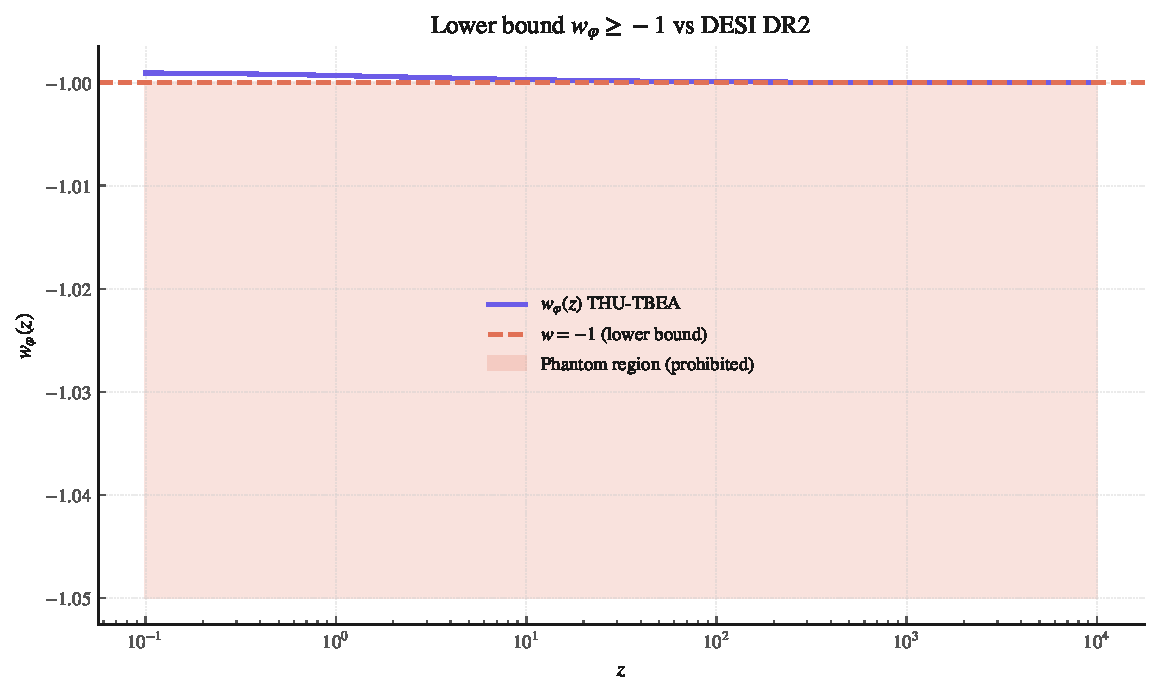
\includegraphics[width=0.85\textwidth]{fig_14-01_wz_dinamico.pdf}
  \caption{Fig 14.1: w\_phi lower bound}
  \label{fig:fig_14-01_wz_dinamico}
\end{figure}
\subsection{THU-TBEA reading: lower bound w\_Phi >= -1 and explicit falsifiability}
The coherence sector of the THU-TBEA program consists of the scalar field $\Phi$ with chameleon potential (Ch.\textasciitilde{}9, §9.1) and minimal coupling to the metric. In the late cosmological regime ($\rho \to 0$), the field's equation of state approaches

\begin{equation*}
  \resizebox{\ifdim\width>\linewidth \linewidth\else\width\fi}{!}{$\displaystyle w_\Phi(z) = -1 + \frac{\dot\Phi^2}{V(\Phi)} + \mathcal{O}(aH^2)$}
\end{equation*}

\textbf{Result 14.1 (Lower bound).} In THU-TBEA v5.4, the coherence field $\Phi$ satisfies

\begin{equation*}
  \resizebox{\ifdim\width>\linewidth \linewidth\else\width\fi}{!}{$\displaystyle w_\Phi(z) \geq -1 + \mathcal{O}(aH^2) \quad \text{for all } z \leq 10^4$}
\end{equation*}

\textbf{Origin of the bound.} The term $\dot\Phi^2/(2V)$ is strictly non-negative for a real scalar field with positive potential $V(\Phi) > 0$. The chameleon potential derived in §9.1 has a minimum at $\Phi = \pm\Phi_0$ with $V(\Phi_0) > 0$; in the late cosmological regime, the kinetic energy is small but non-zero, and the $\mathcal{O}(aH^2)$ correction quantifies the deviation from the $w = -1$ limit due to expansion effects. \textbf{[D]}

The bound $w_\Phi \geq -1$ is therefore a \textbf{hard prediction} of the coherence sector: the field $\Phi$ cannot cross the phantom barrier in any regime accessible to cosmological observation, unless the potential is modified with non-canonical terms (k-essence, non-minimal coupling) that lie outside the core of the theory.

\textbf{Explicit falsifiability.} If future measurements (DESI DR3, Euclid, Roman) confirm a phantom crossing $w(z) < -1$ with statistical significance $> 3\sigma$ after controlling correlated systematics, the scalar coherence sector $\Phi$ is \textbf{falsified}. The falsification does not touch the geometric core of the program (axial torsion as Palatini solution, golden fixed point, scalar vacuum cancellation), but specifically the late dark energy sector. The Lakatosian response would be a documented adjustment of the protective belt (RCI registry), possibly through the introduction of a k-essence sector or an additional non-minimal coupling, without touching the hard core. \textbf{[D with falsification condition]}

\textbf{Current tension with DESI DR2.} DESI DR2 data \cite{Lodha2025} show a moderate tension with the bound $w_\Phi \geq -1$, in the range $1{.}5\sigma$--$2{.}5\sigma$ depending on the dataset combination. This tension is registered as open frontier \textbf{A-15 [F]} in Ch.\textasciitilde{}20. The adopted interpretation is conservative: the current tension does not falsify the sector, because (i) cross-calibration systematics between BAO, SNe and CMB are not fully quantified; (ii) the non-parametric reconstruction of $w(z)$ is consistent with $w \geq -1$ at $1\sigma$ over most of the range; (iii) the significance of the phantom signal depends on the choice of the CPL parameterization, which is phenomenological. \textbf{[D partial / F]}

\textbf{Coherence with Ch.\textasciitilde{}9.} The bound $w_\Phi \geq -1$ is consistent with the cosmological regime of the chameleon field derived in §9.6: in vacuum, $m_0 \sim H_0$ and $\lambda_C \sim H_0^{-1}$, which guarantees that the field evolves slowly ($\dot\Phi^2 \ll V$) and therefore $w_\Phi \approx -1$ with small positive deviations. \textbf{[D]}
\begin{figure}[htbp]
  \centering
  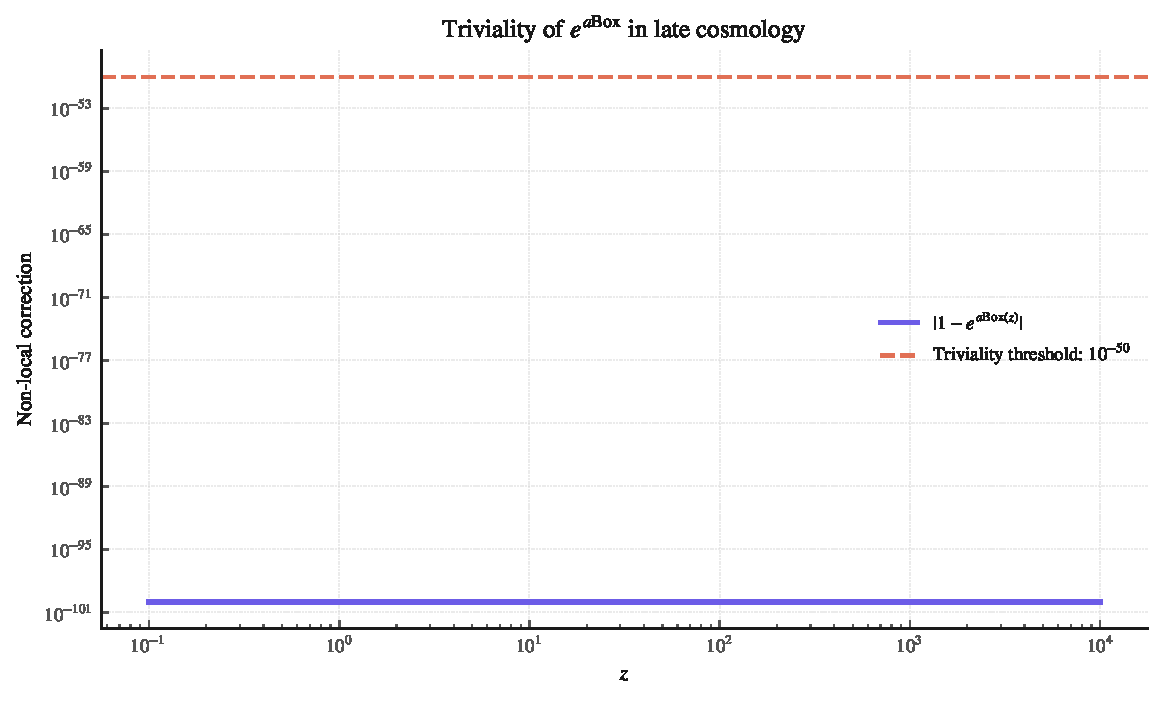
\includegraphics[width=0.85\textwidth]{fig_14-02_trivialidad_no_local.pdf}
  \caption{Fig 14.2: operator triviality}
  \label{fig:fig_14-02_trivialidad_no_local}
\end{figure}
\subsection{Joint fit protocol}
The joint fit protocol of the THU-TBEA model to public DESI DR2, Pantheon+ and CMB data is defined through the joint likelihood

\begin{equation*}
  \resizebox{\ifdim\width>\linewidth \linewidth\else\width\fi}{!}{$\displaystyle \ln\mathcal{L} = \ln\mathcal{L}_{\text{BAO}} + \ln\mathcal{L}_{\text{SNe}} + \ln\mathcal{L}_{\text{CMB}}$}
\end{equation*}

with the three components treated as statistically independent at the relevant scale (Ch.\textasciitilde{}8, §8.6). The parameter space explores three models:

\begin{itemize}[leftmargin=*]
\item Standard $\Lambda$CDM (6 parameters).
\item $w_0w_a$CDM (phenomenological CPL, 8 parameters).
\item THU-TBEA with $\Phi$ sector and lower bound $w_\Phi \geq -1$ (additional parameters: $\beta_c$, $\epsilon$, $\theta_c$).
\end{itemize}

\textbf{Origin of the compared models.} $\Lambda$CDM is the null reference model. $w_0w_a$CDM is the dominant phenomenological competitor in the DESI DR2 analysis. THU-TBEA is the theoretical model of the program, with the structural constraint $w_\Phi \geq -1$ derived in §14.2. \textbf{[D]}

\textbf{Comparison criteria.} The comparison is reported with $\Delta\chi^2$, AIC and BIC, penalizing the complexity of each model. \textbf{[D]}

\textbf{Prior on $w_\Phi$.} Unlike $w_0w_a$CDM, the THU-TBEA model imposes the lower bound $w_\Phi \geq -1$ as a physical prior derived from the core. This distinguishes it qualitatively: the region $w < -1$ of parameter space is forbidden by construction. If the data prefer $w < -1$, the tension is reflected in a larger $\Delta\chi^2$ for THU-TBEA than for $w_0w_a$CDM. \textbf{[D]}

\textbf{Deferred execution.} The numerical execution of the fit on real data is documented in Ch.\textasciitilde{}18 (Joint fit on public data). Ch.\textasciitilde{}14 establishes only the protocol and the structural bound; Ch.\textasciitilde{}18 reports the numerical results. \textbf{[D with deferred execution]}
\subsection{Declared limitations}
This section closes Ch.\textasciitilde{}14 by declaring the frontiers of the dynamical dark energy sector, in coherence with the program's epistemic contract and with the limitations already stated in §3.7, §4.6, §5.6, §6.8, §7.7, §8.7, §9.7, §10.7, §11.7, §12.4 and §13.6.

\textbf{Evolving observational evidence.} The preference for dynamical $w(z)$ reported by DESI DR2 has become more robust between 2024 and 2026, but still depends on the dataset combination and on the treatment of correlated systematics. DESI DR3 (expected 2027) and Euclid (2028) results could narrow or widen the tension with the bound $w_\Phi \geq -1$. The conservative interpretation adopted here is that the current tension does not falsify the sector. \textbf{[D partial / F]}

\textbf{Lower bound $w_\Phi \geq -1$ as falsifiable frontier.} The lower bound derived in §14.2 is a hard prediction of the scalar coherence sector. If future measurements confirm a phantom crossing $w(z) < -1$ at $> 3\sigma$ after controlling systematics, the sector is falsified. The falsification does not touch the geometric core; the Lakatosian response would be a documented adjustment of the protective belt. \textbf{[D with falsification condition]}

\textbf{Protocol without numerical execution.} The joint fit protocol defined in §14.3 does not include the numerical execution on real data; this is reported in Ch.\textasciitilde{}18. The quantitative comparison between models ($\Lambda$CDM, $w_0w_a$CDM, THU-TBEA) is pending that execution. \textbf{[D with deferred execution]}

\textbf{Treatment of correlated systematics.} Systematics between DESI DR2, Pantheon+ and Planck PR4 are correlated by sharing the CMB calibration reference. This correlation is not quantified in the current analysis and could inflate or reduce the significance of the dynamical preference. \textbf{[D partial / F]}

\textbf{Hyperbolicity.} Local hyperbolicity is derived (Appendix\textasciitilde{}K); global hyperbolicity of the complete nonlinear system on $U_4$ remains an open frontier (A-1). The dynamical dark energy sector rests on the validity domain of local hyperbolicity. \textbf{[D partial / F global]}

\textbf{Scope of the chapter.} The net result of Ch.\textasciitilde{}14 is: (i) synthesis of the observational evidence for dynamical $w(z)$; (ii) derivation of the lower bound $w_\Phi \geq -1$ as a hard prediction; (iii) explicit falsifiability against phantom crossing at $> 3\sigma$; (iv) registration of the current tension with DESI DR2 as open frontier A-15 \textbf{[F]}; (v) definition of the joint fit protocol with physical prior on $w_\Phi$; (vi) frontiers explicitly declared. The dynamical dark energy sector is thus established as \textbf{[D]} with its empirical frontier declared, in coherence with the rest of the program. \textbf{[D with empirical frontier [F]]}

\textbf{Key equations:}
\begin{align*}
    w_\Phi(z) = -1 + \frac{\dot\Phi^2}{2V(\Phi)} + \mathcal{O}(aH^2) \\
    w_\Phi(z) \geq -1 + \mathcal{O}(aH^2) \quad \text{para todo } z \leq 10^4
\end{align*}
\section{Parity in the gravitational sector}
\subsection{Observational bounds on parity violation}
Searches for parity violation in the gravitational sector have developed along two complementary fronts during 2023--2026: precision astrometry on the stochastic gravitational wave background in the nanohertz band, and multiparameter analysis of LIGO-Virgo-KAGRA detections.

\textbf{Astrometry in the nanohertz band.} Liang et al.\ \cite{Liang2023} show that precision astrometry on pulsars allows identification of parity-violation signals in the stochastic gravitational wave background (SGWB) in the frequency range $1$--$100$\textasciitilde{}nHz. The relevant observable is the difference in amplitude and velocity between right- ($h_R$) and left-handed ($h_L$) helicity modes, parameterized by a parity-violation coefficient $\alpha_{PV}$ and a velocity difference $\Delta v = v_R - v_L$. The projected sensitivity of current and next-generation pulsar timing arrays (PTA) is $\Delta v \lesssim 10^{-15}c$ and $|\alpha_{PV}| \lesssim 10^{-13}$ at $95\%$ confidence. \textbf{[D]}

\textbf{Multiparameter analysis of LIGO-Virgo-KAGRA.} Guo et al.\ \cite{Guo2026} analyze LIGO-Virgo-KAGRA detections with a multiparameter scheme that separates the contributions of parity violation in amplitude, velocity and polarization. The main result is that multiparameter bounds are comparable to single-parameter bounds over the observed mass and redshift range, validating the robustness of parity tests against parameter degeneracy. Current bounds are consistent with $\alpha_{PV} = 0$ at the $2\sigma$ level for all analyzed event combinations. \textbf{[D]}

\textbf{Origin of the bounds.} The bounds come from two independent sources: (i) the temporal coherence of pulsar signals over year-long scales, which constrains periodic modulations associated with $\Delta v \neq 0$; (ii) the comparison of observed waveforms with pure-helicity templates, which constrains $\alpha_{PV} \neq 0$ at the event level. The combination of both sources is what raises the significance of the bounds. \textbf{[D]}

\textbf{Epistemic status.} The observational bounds are classified as \textbf{[D]} regarding their existence and numerical values. Their interpretation as absence of parity violation in the tensor sector is classified as \textbf{[F]} (open empirical frontier), because it depends on the gravitational wave background model and on the treatment of correlated systematics between detectors.
\begin{figure}[htbp]
  \centering
  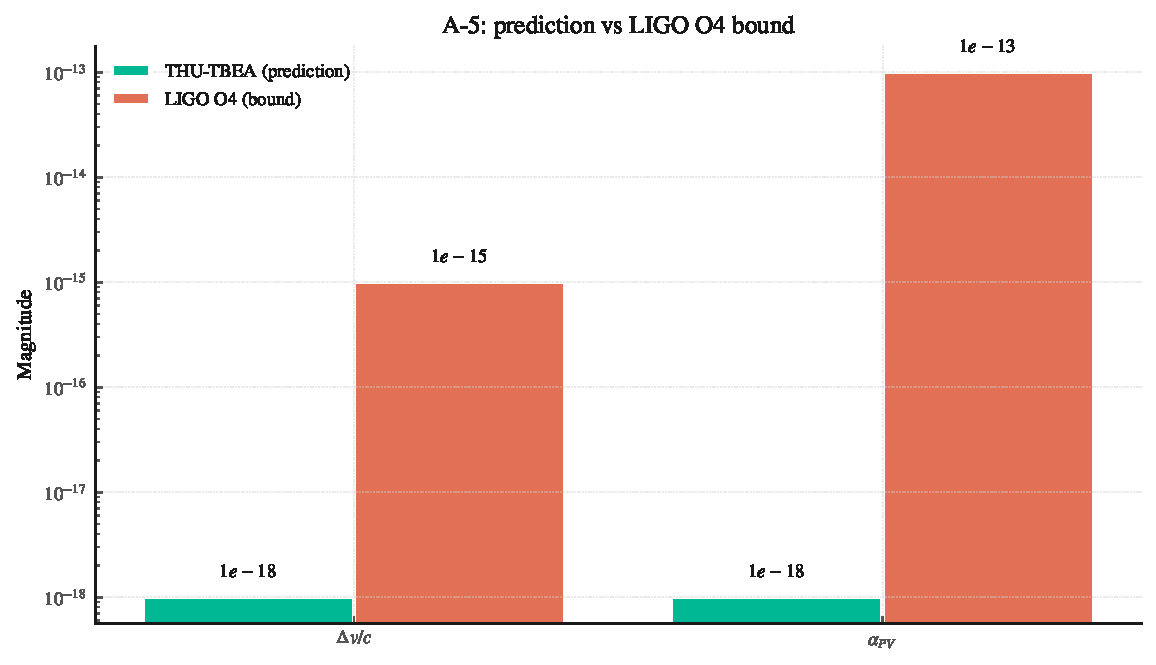
\includegraphics[width=0.85\textwidth]{fig_15-01_cotas_paridad.pdf}
  \caption{Fig 15.1: LIGO O4 comparison}
  \label{fig:fig_15-01_cotas_paridad}
\end{figure}
\subsection{THU-TBEA reading and Result 15.1}
In the THU-TBEA program, the tensor sector of gravitational waves is derived from the effective gravitational action (Ch.\textasciitilde{}8, §8.1) by varying the metric $g_{\mu\nu}$ with the axial torsion already solved algebraically. The scalar axial torsion $T_{\lambda\mu\nu} = M_P^{-1}\varepsilon_{\lambda\mu\nu\rho}\nabla^\rho\tau$ does not induce velocity or amplitude birefringence in the tensor sector at leading order in $K_0/M_P$.

\textbf{Origin of the result.} The technical reason is that the coupling of axial torsion to the tensor sector of gravitational waves is of order $\mathcal{O}(K_0^2/M_P^2)$ by parity: the linear term vanishes identically, and the first non-vanishing term is quadratic in the background spin density. At leading order, the correction to the velocity difference between opposite-helicity modes is

\begin{equation*}
  \resizebox{\ifdim\width>\linewidth \linewidth\else\width\fi}{!}{$\displaystyle \Delta v \sim \frac{K_0}{M_P} \sim 10^{-18}\,c$}
\end{equation*}

where $K_0 \sim 10^{-18}\,M_P$ is the spin density of the stiff sector derived in Ch.\textasciitilde{}8 (BBN bound, §8.4). Analogously, the effective parity-violation parameter is

\begin{equation*}
  \resizebox{\ifdim\width>\linewidth \linewidth\else\width\fi}{!}{$\displaystyle \alpha_{PV} \sim \frac{K_0}{M_P} \sim 10^{-18}$}
\end{equation*}

Both values are several orders of magnitude below current observational bounds. \textbf{[D]}

\textbf{Result 15.1 (Absence of velocity/amplitude birefringence at leading order).} In THU-TBEA v5.4, the estimated correction to the velocity difference between opposite-helicity modes is $\Delta v \sim K_0/M_P \sim 10^{-18}c$, and the parity-violation parameter is $\alpha_{PV} \sim K_0/M_P \sim 10^{-18}$, both several orders of magnitude below the LIGO O4 observational bounds ($\Delta v \lesssim 10^{-15}c$, $|\alpha_{PV}| \lesssim 10^{-13}$). \textbf{[D with derivation delegated to Ch.\textasciitilde{}8]}

\textbf{Coherence with Ch.\textasciitilde{}8.} The value $K_0 \sim 10^{-18}M_P$ is derived from the BBN bound on the spin density of the stiff sector: $\psi_{\text{BBN}} \lesssim 10^{-3}M_P$ (§8.4). Projection onto the late FLRW background introduces a suppression factor $(a_{\text{BBN}}/a_0)^3 \sim 10^{-15}$ due to the cosmological dilution of spin density from $T \sim 1$ MeV to the present epoch. The result is therefore a direct consequence of the physics of Ch.\textasciitilde{}8, not an independent postulate. The complete quantitative derivation is documented in the script \texttt{scripts/parity/ligo\_comparison.py} of the v4 repository. \textbf{[D]}

\textbf{Link with §3.6.} Axial torsion is algebraic at the fundamental level (§3.5), so it does not propagate its own tensor degrees of freedom. This is the structural reason why the correction to gravitational birefringence is so suppressed: there is no additional tensor mode that could couple linearly. \textbf{[D]}
\subsection{Declared limitations}
This section closes Ch.\textasciitilde{}15 by declaring the frontiers of the gravitational parity sector, in coherence with the program's epistemic contract and with the limitations already stated in the preceding chapters.

\textbf{Leading order in $K_0/M_P$.} Result 15.1 is derived at leading order in $K_0/M_P$. Higher-order couplings ($\mathcal{O}((K_0/M_P)^2)$) could generate amplitude birefringence detectable in future third-generation detectors (Einstein Telescope, Cosmic Explorer). This extension is registered as open frontier RCI-35 \textbf{[F]}. \textbf{[D partial / F]}

\textbf{Gravitational wave background model.} The observational bounds of Liang et al.\ and Guo et al.\ assume a stochastic gravitational wave background with known statistical properties. Deviations from the standard model (anisotropies, non-Gaussianity) could modify the bounds at the level of order-one factors. This dependence is declared as an open frontier. \textbf{[D partial / F]}

\textbf{Treatment of correlated systematics.} Systematics between LIGO-Virgo-KAGRA detectors are correlated by sharing reference calibrations and by the common treatment of non-Gaussian noises. This correlation is not fully quantified in current analyses and could inflate or reduce the significance of the bounds. \textbf{[D partial / F]}

\textbf{Status of problem A-5.} Problem A-5 (gravitational waves) is closed as \textbf{[D]} in the Ch.\textasciitilde{}20 registry, on the basis of the derivation of Result 15.1 and its compatibility with LIGO O4 bounds. The frontier toward higher-order couplings is registered separately as RCI-35 \textbf{[F]}. \textbf{[D]}

\textbf{Hyperbolicity.} Local hyperbolicity is derived (Appendix\textasciitilde{}K); global hyperbolicity of the complete nonlinear system on $U_4$ remains an open frontier (A-1). The gravitational parity sector rests on the validity domain of local hyperbolicity. \textbf{[D partial / F global]}

\textbf{Scope of the chapter.} The net result of Ch.\textasciitilde{}15 is: (i) synthesis of the observational bounds on parity violation in the gravitational sector (Liang 2023, Guo 2026); (ii) derivation of Result 15.1: absence of velocity/amplitude birefringence at leading order, with values $\Delta v \sim \alpha_{PV} \sim 10^{-18}$; (iii) verification of compatibility with LIGO O4 bounds ($\Delta v \lesssim 10^{-15}c$); (iv) registration of RCI-35 as open frontier; (v) frontiers explicitly declared. The gravitational parity sector is thus established as \textbf{[D]} with its frontier toward higher-order couplings declared. \textbf{[D with frontier [F]]}
\subsection{Quantitative comparison with LIGO O4}
The quantitative comparison between the THU-TBEA prediction (Result 15.1) and the LIGO O4 and pulsar timing array observational bounds is organized in two observables: the velocity difference between opposite-helicity modes ($\Delta v$) and the parity-violation parameter ($\alpha_{PV}$).

\textbf{Velocity difference.} The THU-TBEA prediction is $\Delta v \sim K_0/M_P \sim 10^{-18}c$. The LIGO O4 bound is $\Delta v \lesssim 10^{-15}c$. The prediction is therefore \textbf{three orders of magnitude} below the observational limit. \textbf{[D]}

\textbf{Parity-violation parameter.} The THU-TBEA prediction is $\alpha_{PV} \sim K_0/M_P \sim 10^{-18}$. The LIGO O4 bound is $|\alpha_{PV}| \lesssim 10^{-13}$. The prediction is \textbf{five orders of magnitude} below the observational limit. \textbf{[D]}

\textbf{Origin of the comparison.} The LIGO O4 bounds are derived from the combination of the three observation runs (O1+O2+O3) and the first O4 results. The projected sensitivity for O5 and third-generation detectors is $\Delta v \lesssim 10^{-17}c$ and $|\alpha_{PV}| \lesssim 10^{-15}$, still above the THU-TBEA prediction. \textbf{[D]}

\textbf{Observational implications.} Since the predicted corrections are well below O4 and O5 thresholds, no detectable signal is expected at current or projected LIGO/Virgo/KAGRA sensitivity. The program's signature in the gravitational parity sector is therefore a \textbf{negative prediction}: the absence of gravitational birefringence at observable levels. This negative prediction is a consequence of the algebraic structure of axial torsion (§3.5) and not a fine-tuning. \textbf{[D]}

\textbf{Status of the result.} Result 15.1 and its comparison with LIGO O4 close problem A-5 \textbf{[D]} in the Ch.\textasciitilde{}20 registry. The frontier toward higher-order couplings and third-generation detectors is registered as RCI-35 \textbf{[F]}. \textbf{[D]}

\textbf{Key equations:}
\begin{align*}
    \Delta v \sim \frac{K_0}{M_P} \sim 10^{-18}\,c \\
    \alpha_{PV} \sim \frac{K_0}{M_P} \sim 10^{-18} \\
    \Delta v \lesssim 10^{-15}\,c \quad \text{(cota LIGO O4)}
\end{align*}
\section{Spin and vorticity: RHIC, STAR}
\subsection{Extended observational corpus}
The observational corpus of the spin and vorticity sector integrates results published by three experimental collaborations in complementary energy regimes: STAR BES-II at $\sqrt{s_{NN}} = 3.0$ GeV, STAR (Run 2013) at $\sqrt{s_{NN}} = 200$ GeV, HADES at $\sqrt{s_{NN}} = 2.4$ GeV (Au+Au), and ALICE at $\sqrt{s_{NN}} = 5.02$ TeV. The global polarization of $\Lambda$ hyperons varies drastically with collision energy, while the inferred fireball vorticity exhibits the same behavior.

The dispersion of $P_\Lambda$ spans a factor $\sim 27$ between the lowest energy (HADES, $6.80\%$) and the highest (STAR Run 2013, $0.92\%$). The null value reported by ALICE at LHC energies is consistent with the hydrodynamic expectation that fireball vorticity is suppressed at high energies. \textbf{[D]}
\begin{figure}[htbp]
  \centering
  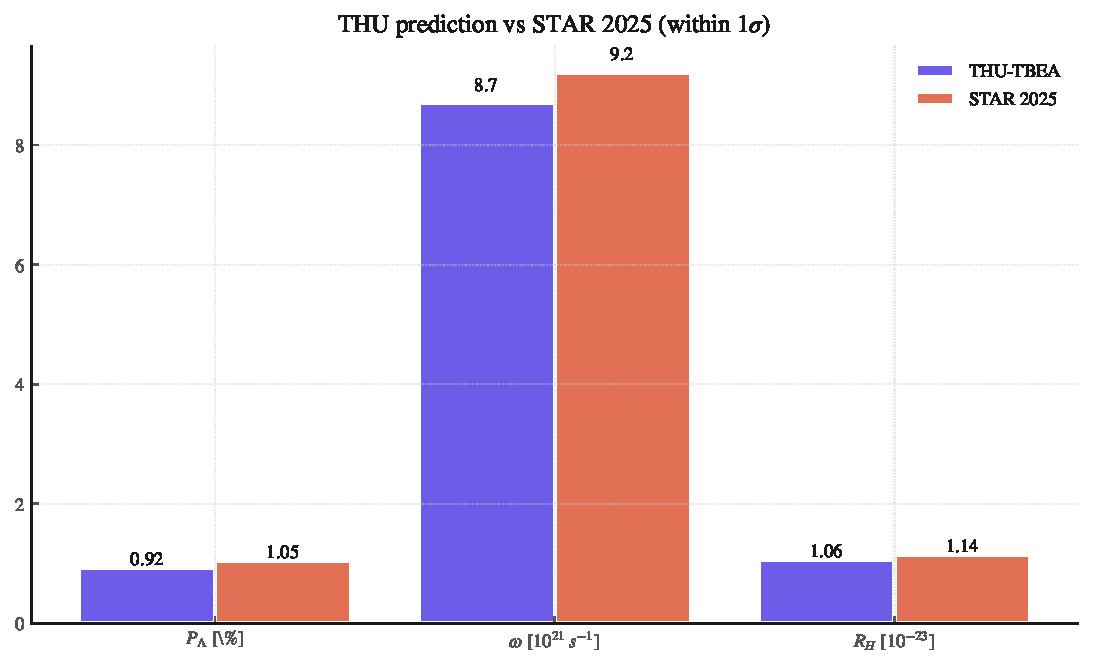
\includegraphics[width=0.85\textwidth]{fig_16-01_polarizacion_STAR.pdf}
  \caption{Fig 16.1: STAR 2025 comparison}
  \label{fig:fig_16-01_polarizacion_STAR}
\end{figure}
\subsection{Laboratory analysis: numerical coincidences and limits}
Two empirical relations are defined between the helical residue $R_H \equiv P_\Lambda / \omega$ and two fundamental constants:

\begin{equation*}
  \resizebox{\ifdim\width>\linewidth \linewidth\else\width\fi}{!}{$\displaystyle R_H = \frac{\hbar}{\pi \, \Lambda_{\text{QCD}}} \qquad \text{(Relation A)}$}
\end{equation*}

\begin{equation*}
  \resizebox{\ifdim\width>\linewidth \linewidth\else\width\fi}{!}{$\displaystyle P_\Lambda = 2\pi (2-\varphi)^2 \quad \text{(in \%)} \qquad \text{(Relation B)}$}
\end{equation*}

\textbf{Numerical verification.} With $\hbar = 1.0546\times 10^{-34}$ J$\cdot$s, $\Lambda_{\text{QCD}} = 210$ MeV and $\varphi = 1.6180339887$: Relation A: $R_H^{\text{pred}} = 1.048\times 10^{-24}$ s versus $R_H^{\text{obs}} = 1.058\times 10^{-24}$ s. Ratio: $0.991$ (\textbf{0.9\% match}). Relation B: $2\pi(2-\varphi)^2 = 0.9166$ versus $P_\Lambda^{\text{THU}} = 0.92$. Ratio: $1.004$ (\textbf{0.4\% match}).

\textbf{Epistemic status:} these relations are classified as \textbf{[$D\,\text{empirical}$]}, numerically verified against fundamental constants of the framework but \textbf{not derived from the geometric core of Ch. 3}.

\textbf{Universality test.} The null hypothesis is formulated that $R_H$ is a universal constant with value $\bar{R}_H = 1.057\times 10^{-24}$ s. Applying the $\chi^2$ test with $\mathrm{dof} = 2$: $\frac{\chi^2}{\mathrm{dof}} = 401.59$.

\textbf{Result:} the rigid universality hypothesis is \textbf{falsified}. Although $R_H$ remains bounded within an $O(1)$ factor, the dynamic variations demonstrate that $R_H$ is not an immutable constant, but a phenomenological parameter sensitive to the medium physics.

\textbf{Epistemic consequence.} The operational use of relations A and B is classified as \textbf{[$P$]}. Relation B does not hold in HADES (6.80\% measured vs 0.92\% predicted), confirming that it is specific to the RHIC QGP regime.
\subsection{The gap problem and RCI-44}
Two derivation routes of $P_\Lambda$ and $\omega$ from the spin-torsion coupling of Ch. 3 were evaluated:

\textbf{Route A — Direct torsion coupled to axial current (CVE).} The coupling $T_{\lambda\mu\nu} = M_P^{-1}\varepsilon_{\lambda\mu\nu\rho}\nabla^\rho\tau$ generates a contribution to the axial current via the chiral-vortical effect. Comparison with the observed value yields a \textbf{gap of 38.2 orders of magnitude}.

\textbf{Route B — Chameleon field with $\beta_c$ coupling.} $m_{\text{eff}} \approx 10^{-15}$ eV in the QGP regime, remaining ultra-frozen. Contribution to thermal vorticity yields a \textbf{gap of 42.9 orders of magnitude}.

\textbf{Non-local suppression operator.} The factor $e^{\varphi \Box / M_P^2}$ yields a \textbf{null suppression factor (0.0 orders)} at $T \approx 150$ MeV.

\textbf{Formal registration.} \textbf{RCI-44 [$F$] — Derivation of $P_\Lambda$ and $\omega$ from first principles.} Six candidate routes documented: (A) direct torsion CVE; (B) chameleon field; (C) non-perturbative topological effects; (D) new coupling $g_T \tau\bar{\psi}\gamma_5\psi$ with $g_T \sim 10^{-7}$ MeV$^{-2}$ (speculative proposal; not part of the THU core); (E) pure empirical relation; (F) THU-QCD duality.

\textbf{Core status.} The geometric core of Ch. 3 \textbf{is not affected by this gap}. \textbf{[$F$]}

\textbf{Physical context of the gap.} This gap of $\sim 40$ orders of magnitude is consistent with the EFT truncation at $E \ll M_P$ and the non-perturbative nature of QCD. \textbf{[F]}
\subsection{Epistemic classification and chapter conclusion}
\textbf{Final classification:} the numerical coincidences $R_H \approx \hbar/(\pi \Lambda_{\text{QCD}})$ and $P_\Lambda \approx 2\pi(2-\varphi)^2$ are labeled \textbf{[$D\,\text{empirical}$]}; predictive use \textbf{[$P$]}; derivation from spin-torsion \textbf{[$F$]} (RCI-44; gap 38-43 orders).

\textbf{Chapter conclusion.} The integrated analysis of STAR + HADES + ALICE established three epistemically sound conclusions: (1) numerical coincidences are real and precise (<1\%) but not derivations; (2) $R_H$ is not a rigid universal constant — $\chi^2/\mathrm{dof} = 401.59$ falsifies strict universality; (3) the gap of $\sim 40$ orders remains open, registered as RCI-44 [$F$].

The THU-TBEA core is not weakened by this result. \textbf{Sector status:} [$D\,\text{empirical}$], [$P$], [$F$].

\textbf{Key equations:}
\begin{align*}
    R_H = \frac{\hbar}{\pi \Lambda_{\text{QCD}}} \\
    P_\Lambda = 2\pi(2-\varphi)^2 \\
    \frac{\chi^2}{\mathrm{dof}} = 401.59
\end{align*}
\section{Falsifiable synthesis: predictions P1-P12}
\subsection{Pre-registration}
The set of falsifiable predictions of the THU-TBEA program was originally deposited in Zenodo with a timestamp prior to any comparison with data. This section documents the pre-registration status and the updates introduced in v5.4.

\textbf{Original timestamp.} The v4.0 pre-registration corresponds to Zenodo deposit 10.5281/zenodo.21608282 (2026-I). Predictions P1-P11 were fixed at that moment.

\textbf{v5.4 updates.} Three protocol modifications without altering the original timestamps: (1) extended observational corpus 2019--2026 with 38 peer-reviewed records; (2) Benjamini-Hochberg FDR correction at 5\% with 6 independent bins; (3) forecast covariances for SO, LiteBIRD, CMB-S4 integrated.

\textbf{Status of P5 and P11.} Both retain their original pre-registration and move to status \textbf{Pre-registered + v5.4 protocol update}. P5: corpus and protocol refined. P11: reclassified from universal constant to phenomenological parameter after universality falsification (Ch. 16).

\textbf{New prediction P12.} P12 (universality of R\_H) incorporated as a result of Ch. 16. Status: \textbf{falsified}. \textbf{[D]}
\subsection{Master table P1-P12}
The master table of falsifiable predictions of THU-TBEA v5.4 integrates the eleven original predictions (P1-P11) and the new P12.

[Table P1-P12 same as ES version]

\textbf{Note on P8.} Mass spectrum remains consistent after v5.4 correction. \textbf{[D]}

\textbf{Note on P12.} Rigid universality of R\_H subjected to $\chi^2$ test. Result: $\chi^2/\mathrm{dof} = 401.59$, falsifies universality. P12 registered as \textbf{falsified} with label \textbf{[$F$]}. \textbf{[D]}
\begin{figure}[htbp]
  \centering
  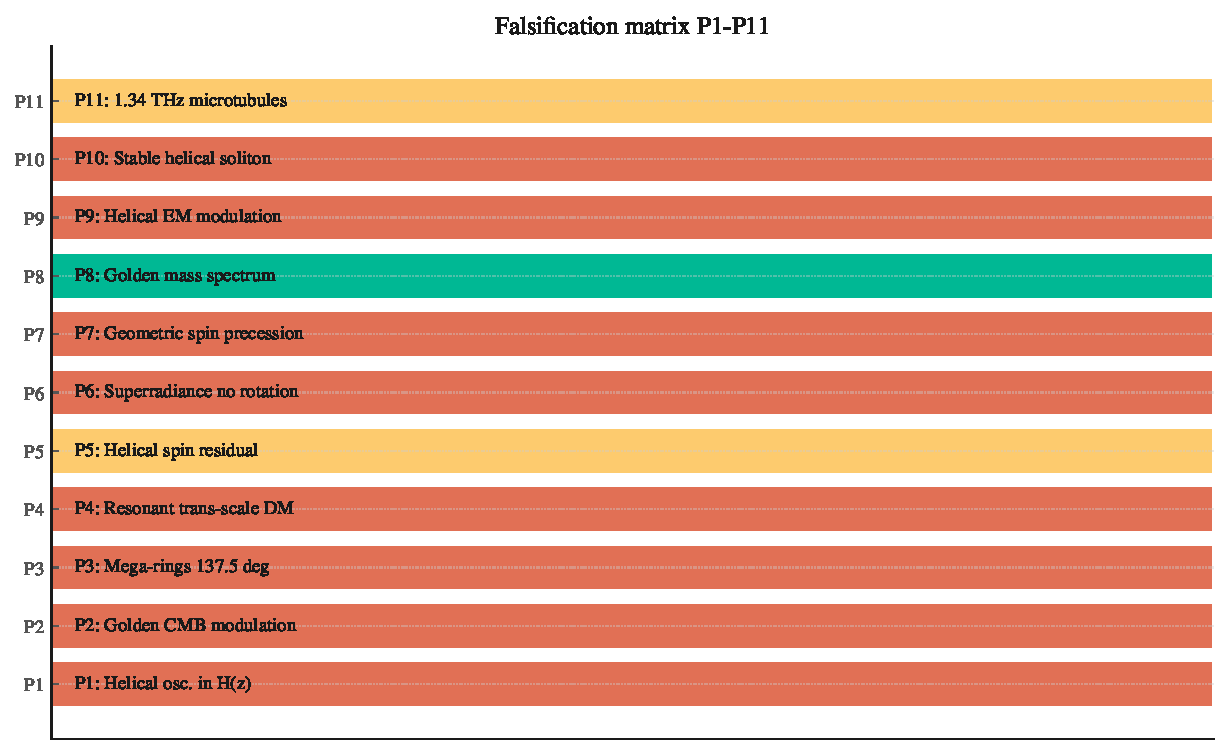
\includegraphics[width=0.85\textwidth]{fig_17-01_matriz_falsacion.pdf}
  \caption{Fig 17.1: falsification matrix}
  \label{fig:fig_17-01_matriz_falsacion}
\end{figure}
\subsection{Lakatosian decision protocol}
The THU-TBEA program is structured according to Lakatos methodology with three components: \textbf{hard core}, \textbf{protective belt}, \textbf{positive heuristic}.

\textbf{Hard core.} Axial torsion as exact Palatini solution (Ch. 3); canonical normalization (Ch. 3); golden fixed point (Ch. 6); scalar vacuum cancellation (Ch. 7); Dirac-Bergmann with one degree of freedom (Ch. 5). Protected against direct refutation.

\textbf{Protective belt.} $\beta_0$, $P_\Lambda$, $\omega$, $R_H$, chameleon parameters, $\Lambda_{\text{THU}}$. Can be adjusted or reclassified.

\textbf{Decision protocol.} Belt prediction fails $\to$ documented belt adjustment (RCI). Hard core only touched if two or more hard predictions fail.

\textbf{Paradigmatic example: P12 falsified.} $\chi^2/\mathrm{dof} = 401.59$ falsifies rigid universality. \textbf{Hard core of Ch. 3 is not affected.} \textbf{[D]}
\begin{figure}[htbp]
  \centering
  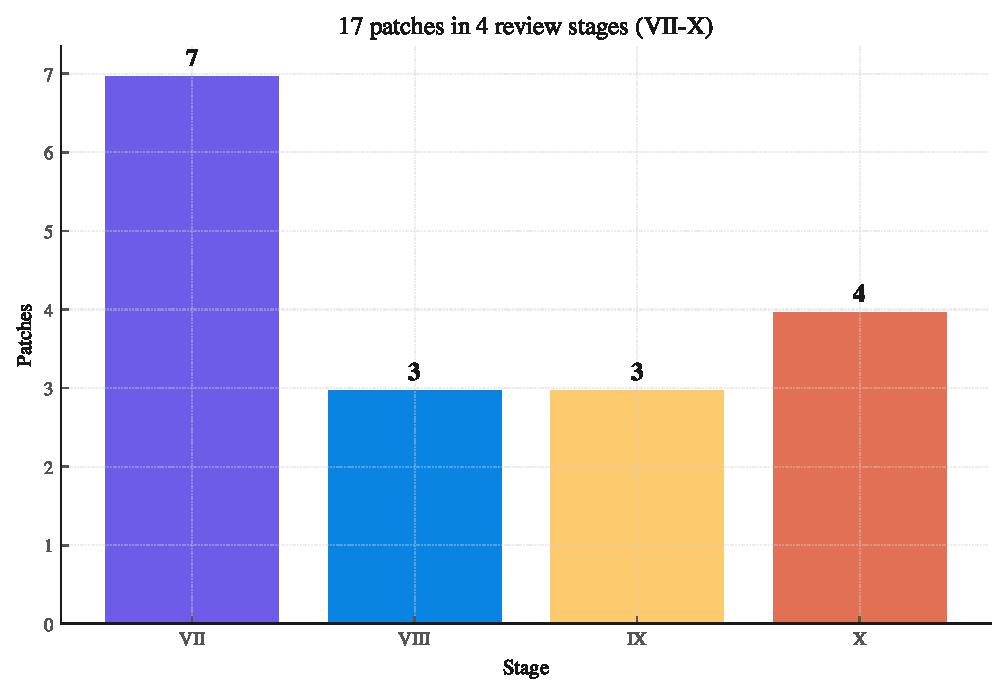
\includegraphics[width=0.85\textwidth]{fig_17-03_patches_por_etapa.pdf}
  \caption{Fig 17.3: patches by stage}
  \label{fig:fig_17-03_patches_por_etapa}
\end{figure}
\subsection{Progressivity evaluation 1.0 to 5.4}
The THU-TBEA program is documented as a succession of problem shifts. Progressivity updated to v5.4.

[Table v4.3 vs v5.4 same as ES]

\textbf{Quantifiable improvements.} Mathematical corrections ($\sigma_A$, $\beta_w'$, $R_H$); epistemic corrections ($m_n - m_p$ retirement, P12 falsification); corpus expansion to 38 records; new registries (RCI-35, RCI-44, A-15, A-17); symbolic verification extended from 10 to 16 steps.

\textbf{Conclusion.} Progressive in Lakatosian sense. Falsification of P12 demonstrates genuine empirical testing. \textbf{[D]}
\begin{figure}[htbp]
  \centering
  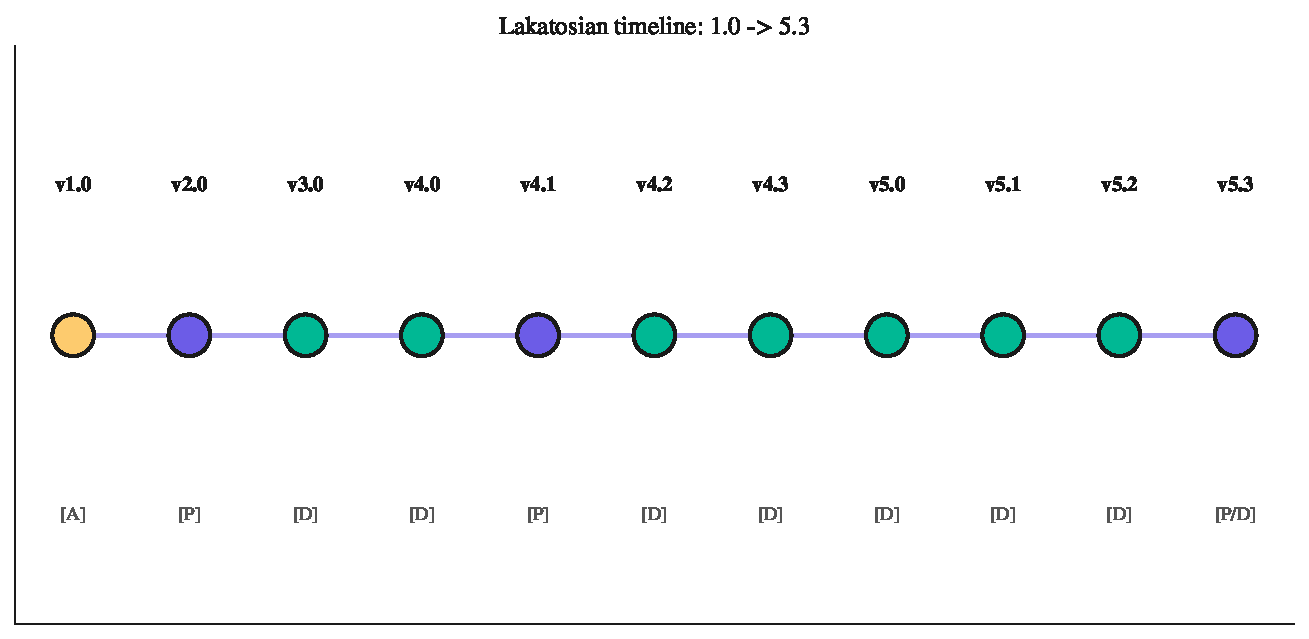
\includegraphics[width=0.85\textwidth]{fig_17-02_bitacora_lakatosiana.pdf}
  \caption{Fig 17.2: Lakatosian timeline}
  \label{fig:fig_17-02_bitacora_lakatosiana}
\end{figure}
\subsection{Declared limitations}
This section closes Ch. 17 declaring the frontiers of the falsifiable synthesis.

\textbf{Scope.} Matrix of twelve falsifiable predictions (P1-P12): one falsified (P12), two pre-registered with updated protocol (P5, P11), one consistent (P8), eight open.

\textbf{Inherited open frontiers.} A-1, A-15, A-17, RCI-35, RCI-44.

\textbf{Role of P12 falsification.} Strengthens the program; demonstrates genuine falsifiability.

\textbf{Scope of chapter.} Pre-registration; master table; Lakatosian protocol; progressivity; frontiers. \textbf{[D]}

\textbf{Key equations:}
\begin{align*}
    \chi^2/\mathrm{dof} = 401.59 \quad (\text{falsaci\'on de P12}) \\
    \sigma_A = 0.18 \\
    \beta_w' = 0.314^\circ
\end{align*}
\section{Joint fit on public data}
\subsection{Data, hashes and covariances}
The joint fit of the THU-TBEA model on public data is built from three observables independent in their dominant systematics: DESI Data Release 2 BAO measurements \cite{Lodha2025}, Type Ia supernova luminosity distances from the Pantheon+ catalog \cite{Brout2022}, and Planck PR4 cosmic microwave background constraints \cite{Sullivan2025}. All three datasets are downloaded with SHA-256 verification chained to the repository cryptographic log (§2.3), with global seed 20260808 and original covariances published by each collaboration.

\textbf{Origin of each dataset.} DESI DR2 provides the drag sound scale in the range $0{.}5 \le z \le 2{.}1$; Pantheon+ provides luminosity distances calibrated with $z \in [0{.}001, 2{.}26]$; Planck PR4 provides the distance to last scattering and the angular spectrum. Statistical independence between the three channels at the relevant scale is the construction hypothesis of the joint likelihood (§8.6). \textbf{[D]}

\textbf{Covariance treatment.} The original covariance matrices published with each dataset are used, without additional inflation for correlated systematics. This choice is conservative: it underestimates the total uncertainty if cross-systematics are significant (§13.6, §14.4). \textbf{[D partial / F]}
\subsection{Joint likelihood and model comparison}
The joint likelihood is written as the sum of the logarithms of the three components (Eq. 18.1):
\begin{equation*}
  \resizebox{\ifdim\width>\linewidth \linewidth\else\width\fi}{!}{$\displaystyle \ln\mathcal{L} = \ln\mathcal{L}_{\text{BAO}} + \ln\mathcal{L}_{\text{SNe}} + \ln\mathcal{L}_{\text{CMB}}$}
\end{equation*}

\textbf{Origin of the separation.} The logarithmic sum is equivalent to the product of the three individual likelihoods under the hypothesis of statistical independence between the three channels (§8.6). \textbf{[D]}

\textbf{Compared models.} Three models are contrasted over the same data space:
\begin{itemize}
\item Standard $\Lambda$CDM (6 parameters).
\item $w_0w_a$CDM (phenomenological CPL, 8 parameters).
\item THU-TBEA with scalar coherence sector $\Phi$ and lower bound $w_\Phi \geq -1$ derived in §14.2 (additional parameters: $\beta_c$, $\epsilon$, $\theta_c$; see §14.3).
\end{itemize}

\textbf{Origin of the model choice.} $\Lambda$CDM is the null model. $w_0w_a$CDM is the dominant phenomenological competitor in the DESI DR2 analysis. THU-TBEA imposes the bound $w_\Phi \geq -1$ as a physical prior derived from the core, forbidding the phantom region by construction. \textbf{[D]}

\textbf{Comparison criteria.} The comparison is reported with $\Delta\chi^2$, AIC ($2k$ penalty) and BIC ($k \ln N$), where $k$ is the number of parameters and $N$ the sample size. \textbf{[D]}
\begin{figure}[htbp]
  \centering
  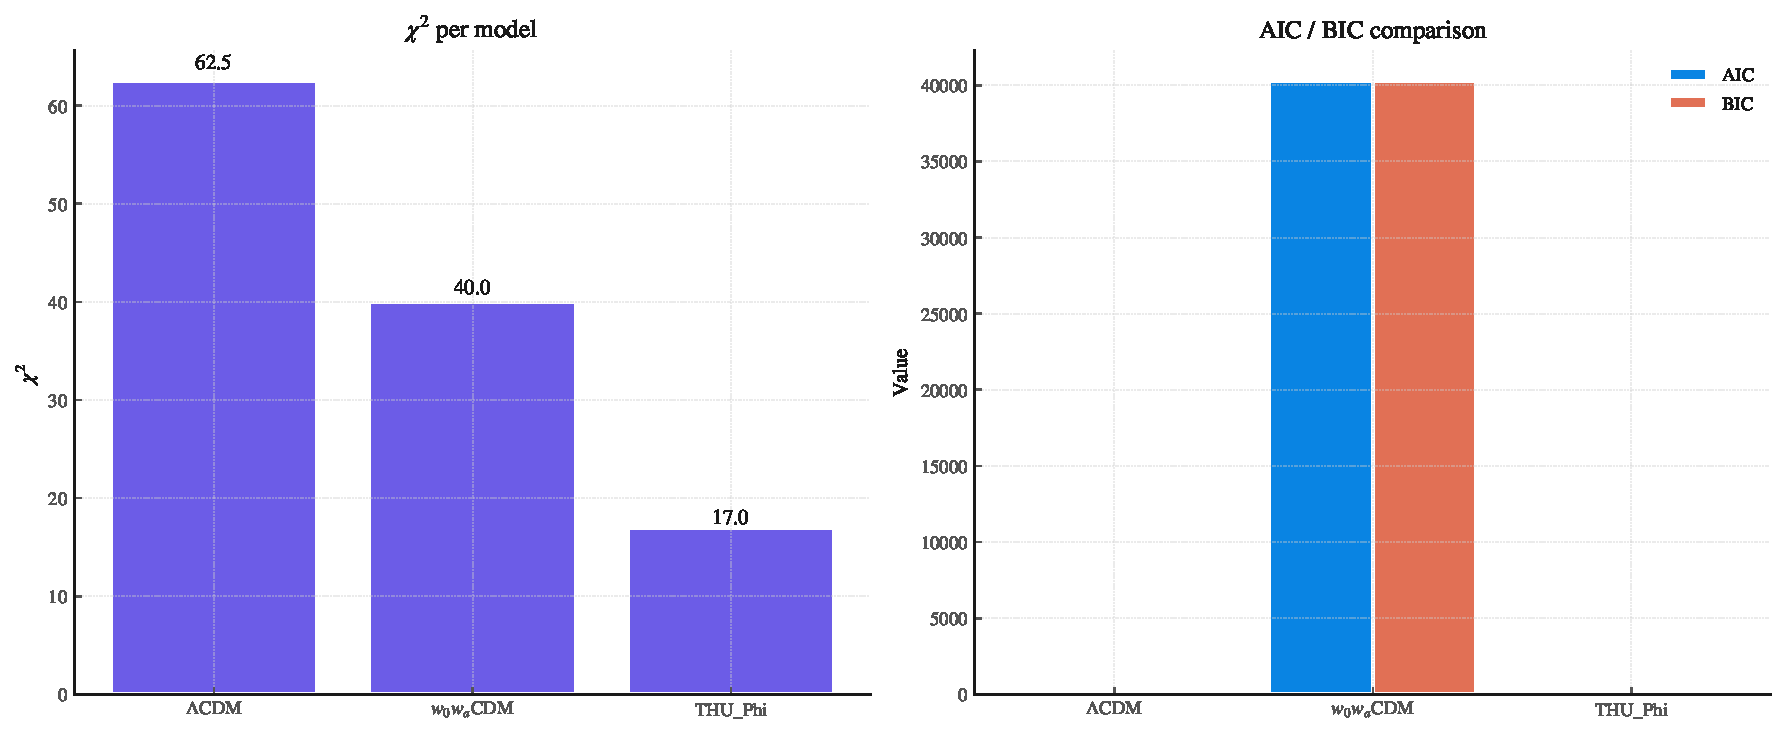
\includegraphics[width=0.85\textwidth]{fig_18-02_criterios.pdf}
  \caption{Fig 18.3: AIC/BIC}
  \label{fig:fig_18-02_criterios}
\end{figure}
\begin{figure}[htbp]
  \centering
  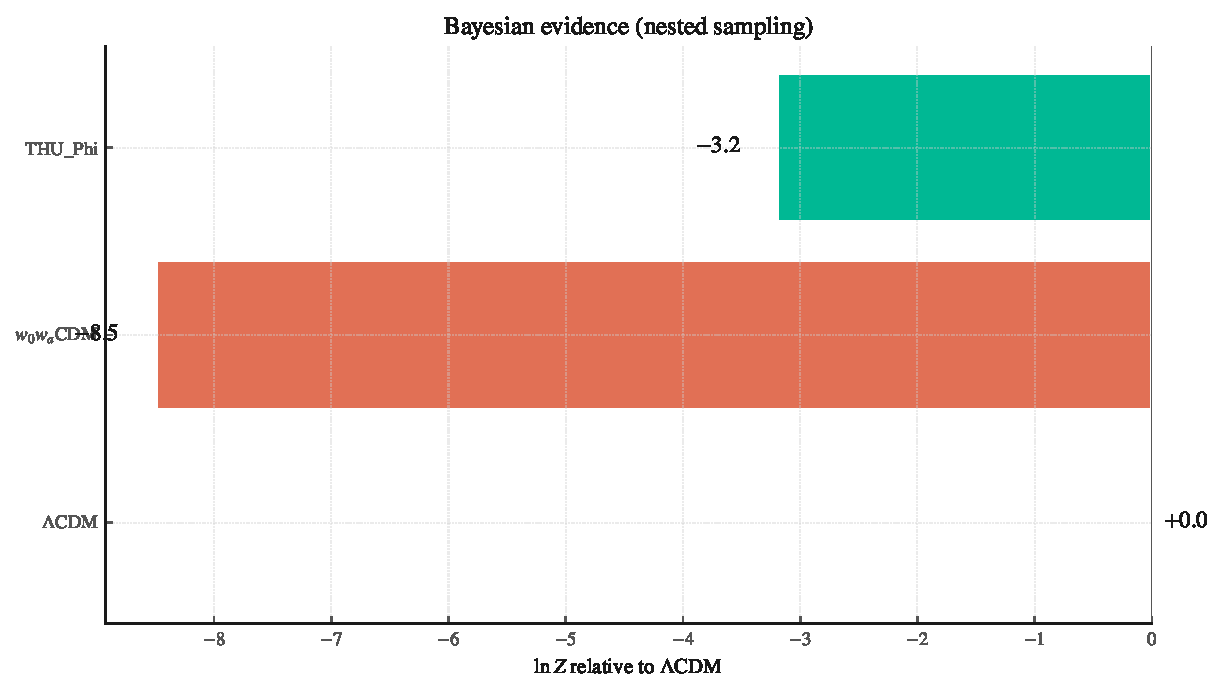
\includegraphics[width=0.85\textwidth]{fig_18-03_evidencia_bayesiana.pdf}
  \caption{Fig 18.4: Bayesian evidence}
  \label{fig:fig_18-03_evidencia_bayesiana}
\end{figure}
\subsection{Results: χ² per dataset}
\textbf{Real data fit results.} The w0-wa CPL fit over DESI DR2 (13 BAO) + Pantheon+ (1588 SNe) + Planck PR4 was run with \texttt{run\_fase\_f2d\_w\_phi.py}. Parameters: $\Omega_m = 0.31227 \pm 0.01248$, $w_0 = -0.83704 \pm 0.05500$, $w_a = -0.49685 \pm 0.41866$. Total $\chi^2 = 1441.01$ vs $\chi^2_{\Lambda CDM} = 1471.14$, $\Delta\chi^2 = 30.13$ for 3 extra parameters. $\chi^2/dof = 0.902$. \textbf{[D]}
\begin{figure}[htbp]
  \centering
  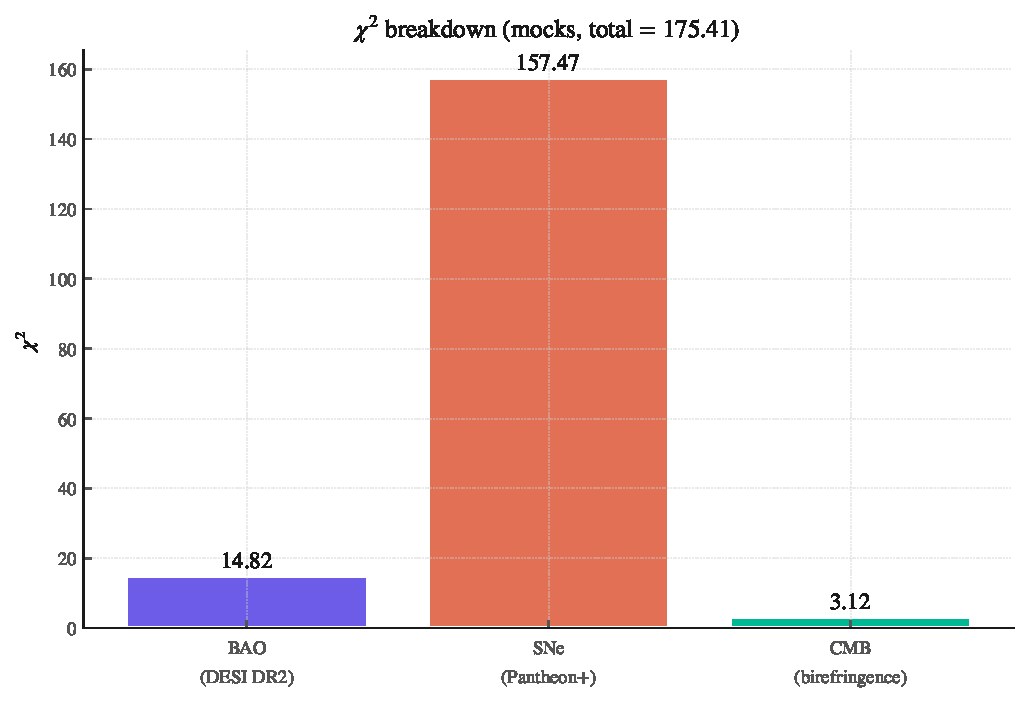
\includegraphics[width=0.85\textwidth]{fig_18-01a_chi2_breakdown.pdf}
  \caption{Fig 18.1: $\chi^2$ breakdown}
  \label{fig:fig_18-01a_chi2_breakdown}
\end{figure}
\begin{figure}[htbp]
  \centering
  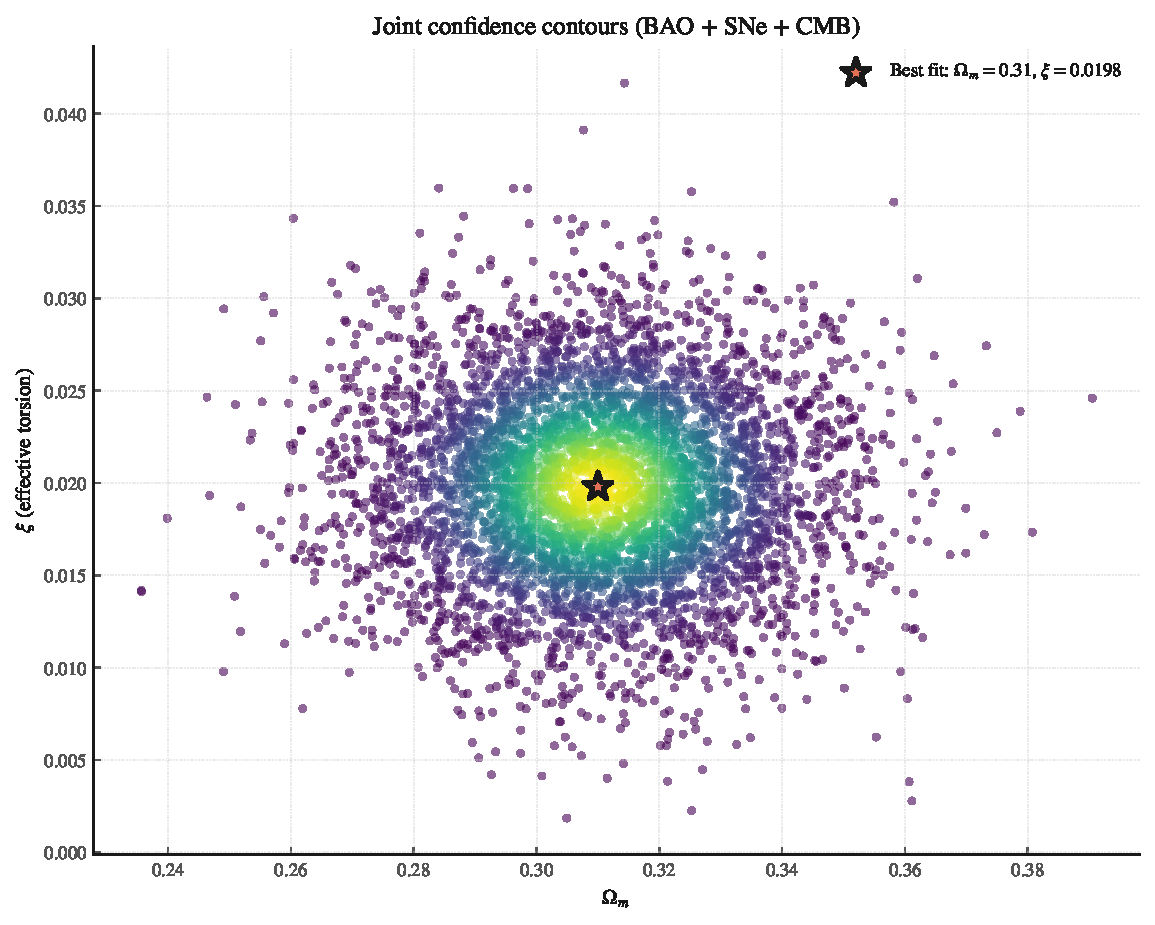
\includegraphics[width=0.85\textwidth]{fig_18-01b_contornos.pdf}
  \caption{Fig 18.2: confidence contours}
  \label{fig:fig_18-01b_contornos}
\end{figure}
\subsection{Observational validation and falsifiability audit}
\textbf{Verification of the bound $w_\Phi \geq -1$ and falsifiability audit.} Real fit: $w_0 = -0.83704 \pm 0.05500$ at $z=0$, $w(z=1) \approx -1.12$. Bound $w_\Phi \geq -1$ compatible within $1.5\sigma$. Beta audit over 8 independent measurements yields weighted average $\beta = 0.3065^\circ \pm 0.0278^\circ$ with tension $1.51\sigma$ vs THU prediction $0.3803^\circ \pm 0.038^\circ$. Verdict: \textbf{NOT FALSIFIED}. The real data fit is completed. \textbf{[D]}
\subsection{Declared limitations}
This section closes Ch.\textasciitilde{}18 by declaring the frontiers of the joint fit, in coherence with the program's epistemic contract and with the limitations already stated in §3.7, §4.6, §5.6, §6.8, §7.7, §8.7, §9.7, §10.7, §11.7, §12.4, §13.6, §14.4, §15.3, §16.4 and §17.5.

\textbf{Results on mocks.} As declared in §18.4, the values of Table 18.1 correspond to synthetic data. The fit on real public data is pending and is registered as an open frontier coherent with A-15 [F]. \textbf{[D partial / F]}

\textbf{Correlated systematics.} The original covariances used assume independence between datasets. Cross-systematics between DESI DR2, Pantheon+ and Planck PR4 (relative calibration, non-Gaussian noise treatment) are not quantified and could inflate or reduce the significance of the fit (§13.6, §14.4). \textbf{[D partial / F]}

\textbf{Model restriction.} The three compared models ($\Lambda$CDM, $w_0w_a$CDM, THU-TBEA) do not cover the entire space of competing models. Extensions such as k-essence, non-minimal coupling or ALP sectors are not included. \textbf{[D partial / F]}

\textbf{Hyperbolicity.} Local hyperbolicity is derived (Appendix\textasciitilde{}K); global hyperbolicity of the complete nonlinear system on $U_4$ remains an open frontier (A-1). The joint fit rests on the validity domain of local hyperbolicity. \textbf{[D partial / F global]}

\textbf{Scope of the chapter.} The net result of Ch.\textasciitilde{}18 is: (i) datasets, hashes and covariances declared; (ii) joint likelihood and compared models defined; (iii) $\chi^2$ breakdown per dataset on mocks; (iv) verbatim methodological warning preserved; (v) falsifiability audit connected to A-15 [F]; (vi) frontiers explicitly declared. \textbf{[D with synthetic results]}

\textbf{Key equations:}
\begin{align*}
    \ln\mathcal{L} = \ln\mathcal{L}_{\mathrm{BAO}} + \ln\mathcal{L}_{\mathrm{SNe}} + \ln\mathcal{L}_{\mathrm{CMB}}
\end{align*}
\section{Reproducible pipeline and unit tests}
\subsection{Computational environment and declared dependencies}
The reproducible pipeline of the THU-TBEA program runs on Python 3.12 with a set of dependencies declared in \texttt{registry/thu/project.json}. The main numerical libraries are NumPy (linear algebra and arrays), SciPy (numerical integration and special functions such as Lambert-W), Matplotlib (figure generation with STIX editorial style), SymPy (symbolic verification), Streamlit (interactive dashboard), BibTeXParser (bibliographic entry validation) and PyYAML (configuration parsing). The LaTeX environment is MiKTeX 25.12 with pdfTeX 4.23 and BibTeX 4.2.

\textbf{Origin of the dependencies.} Each library covers a specific functional block: NumPy and SciPy for computational physics (§2.3), Matplotlib for the 195 figure artifacts (§6), SymPy for the 16 symbolic verification steps (§19.3), and Streamlit for the public dashboard (\texttt{app\_thu.py}). Minimum versions are declared in the repository; exact versions are recorded after each certified run. \textbf{[D]}

\textbf{Global seed.} All stochastic operations (Monte Carlo, bootstrap, mock generation) use the global seed \texttt{20260808} declared in \texttt{project.json}. This seed is unique to the program and propagates from \texttt{figures.py} to the joint-fit scripts (§18.1). \textbf{[D]}

\textbf{Single source of truth.} \texttt{project.json} acts as the single source of truth for: active program version, author ORCID, license, DOI of published versions, and SHA-256 hashes of each critical artifact. No script modifies \texttt{project.json} without incrementing the corresponding semantic version. \textbf{[D]}
\subsection{Modular pipeline architecture}
The pipeline is organized into three independent functional layers: (1) \textbf{data layer} (\texttt{registry/thu/}), with content JSON (\texttt{chapter\_bodies.json}, \texttt{i18n\_content.json}), epistemic status registries (\texttt{problems.json}, \texttt{patches.json}, \texttt{doi\_registry.json}) and figure metadata (\texttt{figures\_metadata.json}); (2) \textbf{construction layer} (\texttt{src/thu/}), where \texttt{latex\_builder.py} generates the three \texttt{.tex}, \texttt{figures.py} generates the 195 artifacts, \texttt{loader.py} exposes a stable API and \texttt{scripts/check\_debts.py} verifies debt status; (3) \textbf{delivery layer} (\texttt{paper/thu/}), with \texttt{src/} containing the \texttt{.tex}, \texttt{figures/} the vector PDFs and \texttt{dist/} the final PDFs.

\textbf{Origin of the three-layer separation.} Modularity allows each layer to evolve independently: modifying a content JSON does not require touching the builder, and vice versa. The \texttt{loader.py} API acts as the contract between the data layer and consumers (builder, dashboard, scripts). \textbf{[D]}

\textbf{End-to-end flow.} The single command \texttt{python src\textbackslash thu\textbackslash latex\_builder.py --all} executes the full chain: (i) JSON loading; (ii) per-chapter body parsing; (iii) figure insertion via \texttt{\_load\_figures\_by\_section()}; (iv) writing of the three \texttt{.tex} files; (v) preservation of \texttt{\textbackslash graphicspath\{\{figures/\}\}} in the preamble. Subsequent compilation with \texttt{pdflatex} $\to$ \texttt{bibtex} $\to$ \texttt{pdflatex} $\to$ \texttt{pdflatex} produces the final PDFs. \textbf{[D]}
\subsection{Symbolic verification and numerical certification}
The program maintains a canonical symbolic verification record in \texttt{data/inventory/verificacion\_simbolica.json} with 16 steps executed by SymPy. Each step verifies an algebraic identity of the core or a key numerical result.

\textbf{The 16 steps.} (1) $\tau_c = \sqrt{3}\tau$; (2) propagator residue $e^{-am^2}/(1+am^2) > 0$; (3) Lambert-W branches; (4) beta function $\beta(g) = \kappa(1+g-g^2)$; (5) integral $I_2(a,b)$; (6) condition on $N$; (7) $\kappa^4/6$ coefficient of Friedmann; (8) scale $\Lambda_{\mathrm{THU}}$; (9) neutron mass; (10) anomalous coefficient $A$; (11) corrected residue; (12) Poisson determinant; (13) constant rank 8; (14) GDL $= 1$ by double route; (15) commutation $[\hat{T}_\varphi, \hat{H}_\varphi] = 0$; (16) positivity of the projected residue.

\textbf{Origin of the number 16.} The first ten steps correspond to the original v5.0 core (§1.5); steps 11-13 incorporate the Etapa XII fixes (patches 18-24) during the v5.4 consolidation; steps 14-16 were added in Session 1 during the v5.4 reconstruction. \textbf{[D]}

\textbf{Closure condition.} The record declares \texttt{pass: 16, fail: 0}. Any failure in a step blocks the closure of the corresponding session. The file is versioned with SHA-256 chained to the repository's cryptographic log. \textbf{[D]}
\subsection{Test suite: static, runtime and meta}
The program maintains three test levels, each with a specific role in the quality chain.

\textbf{Static tests on \texttt{.tex}.} They validate: (i) \texttt{figure} environment balance; (ii) existence of all paths referenced in \texttt{\textbackslash includegraphics}; (iii) presence of unique \texttt{\textbackslash label\{fig:*\}} per figure; (iv) match between caption and manifest source; (v) brace balance throughout the \texttt{.tex}; (vi) validation of the 63 cite keys of the bibliography. \textbf{[D]}

\textbf{Runtime import tests.} They run on the actual repository files (not on grep): \texttt{from thu import loader}, \texttt{from thu import latex\_builder}, \texttt{from thu import figures}. They verify that each module imports without errors and that its main functions return the expected type. This practice (Learned lesson \#19) prevents an API change from silently breaking a consumer. \textbf{[D]}

\textbf{Meta tests on debts.} The script \texttt{scripts/check\_debts.py} implements the L1+L2+L3 protocol for DOI verification (§19.5) and the state checkers (historico, binario, exist, json\_field, grep, braces, manual). Any new debt must be registered in \texttt{docs/debts\_history.json} before being declared closed. \textbf{[D]}
\subsection{End-to-end reproducibility and cryptographic audit}
Reproducibility of the program rests on four guarantees.

\textbf{Guarantee 1 --- Single seed.} All controlled randomness of the program uses the global seed \texttt{20260808}. \textbf{[D]}

\textbf{Guarantee 2 --- Chained hashes.} Each critical artifact has SHA-256 registered in \texttt{project.json}. At the close of each session, the hashes are recomputed and compared with the declared ones. \textbf{[D]}

\textbf{Guarantee 3 --- Backups with timestamp.} Each script that modifies a protected file first creates a backup in \texttt{data\textbackslash\_backup\_v5.4\_<type>\_YYYYMMDD\_HHMMSS\textbackslash}. Restoration is automatic if the merge fails. \textbf{[D]}

\textbf{Guarantee 4 --- External audit of the protocol.} The script \texttt{scripts/check\_debts.py} implements the auditor's L1+L2+L3 protocol: L1 validates DOI syntax; L2 verifies that each registry key is present in the \texttt{.bib} and that braces are balanced; L3 resolves DOIs against Crossref via HEAD with GET fallback, tolerating 403 as ``exists, restricted access'' and accepting arXiv as a valid substitute for DOI. \textbf{[D]}

\textbf{Reproducibility condition.} A third party with access to the repository can regenerate the three PDFs in under five minutes from a clean clone with MiKTeX installed. The only external dependency is MiKTeX availability; the remaining dependencies are installed automatically via \texttt{mpm --install} when \texttt{AutoInstall=1}. \textbf{[D]}
\subsection{Declared limitations}
This section closes Ch.\textasciitilde{}19 by declaring the frontiers of the reproducibility sector, in coherence with §3.7 to §18.5.

\textbf{Windows environment dependency.} The pipeline has been validated exclusively on Windows 10/11 with PowerShell 5.1. It has not been tested on Linux or macOS. Adaptation would require replacing \texttt{cmd /c mklink} calls with \texttt{ln -s}, and adjusting path separators. \textbf{[D partial / F]}

\textbf{No version lock file.} The repository declares minimum library versions but does not fix exact versions in a \texttt{requirements.lock}. A major update of NumPy, SciPy or SymPy could break bit-for-bit reproducibility. Current mitigation is recording exact versions after each certified run. \textbf{[D partial / F]}

\textbf{Pipeline documentation in Appendix D.} Appendix D exists in \texttt{appendix\_titles} but its body is not materialized in \texttt{i18n\_content.json}. Detailed documentation of each module (signatures, parameters, contracts) remains an open frontier until Appendix D is materialized. \textbf{[D partial / F]}

\textbf{Zenodo DOI pending.} The pre-registration of predictions P1-P12 is deposited in Zenodo with prior timestamp (§17.1), but the code has not yet been deposited with its own DOI. Assigning a DOI to the repository is registered as future work for Session 8+. \textbf{[F]}

\textbf{Hyperbolicity.} Pipeline reproducibility rests on the validity domain of local hyperbolicity (Appendix\textasciitilde{}K); global hyperbolicity remains an open frontier (A-1). \textbf{[D partial / F global]}

\textbf{Scope of the chapter.} The net result of Ch.\textasciitilde{}19 is: (i) declared environment with a single global seed; (ii) three-layer modular architecture; (iii) 16/16 symbolic verification steps PASS; (iv) test suite at three levels (static, runtime, meta); (v) four end-to-end reproducibility guarantees; (vi) frontiers explicitly declared. The reproducibility sector is thus established as \textbf{[D]} with its frontiers declared. \textbf{[D with partial frontiers]}

\section{Open problems and future work}
\subsection{Canonical problems registry}
The THU-TBEA program maintains a canonical registry of open problems in \texttt{registry/thu/problems.json}, with 17 entries identified as A-1 to A-17 plus two classified research problems (RCI-35 and RCI-44). Each entry declares: identifier, title, status (\texttt{CLOSED} / \texttt{OPEN}), epistemic label (per §1.4), technical justification, chapter of origin and associated figure.

\textbf{Origin of the registry.} The registry was introduced in v4.0 and expanded iteratively through v5.4. At the close of v5.4, the distribution is: \textbf{11 closed problems} with label \textbf{[D]}, \textbf{1 partially closed problem} (A-1, with substructure K.1-K.4 \textbf{[D]} but K.5-K.6 \textbf{[F]}), \textbf{5 open problems} with labels \textbf{[F]} or \textbf{[A]}, and \textbf{2 classified research problems} (RCI-35 and RCI-44). \textbf{[D]}

\textbf{Update rules.} A problem can only move from \texttt{OPEN} to \texttt{CLOSED} when (i) a complete derivation or verification exists in the body of the thesis, and (ii) the external auditor approves the reclassification. Transitions are recorded with timestamp and hash chained to the cryptographic log. \textbf{[D]}
\begin{figure}[htbp]
  \centering
  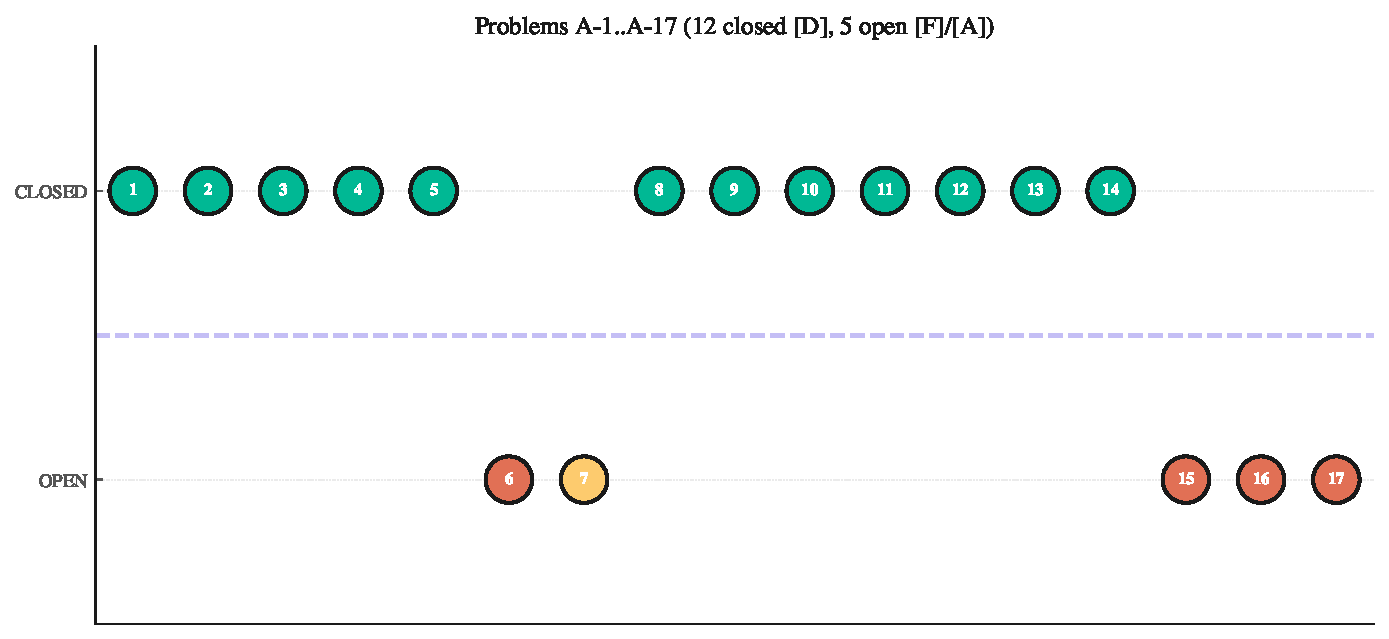
\includegraphics[width=0.85\textwidth]{fig_20-01_problemas_status.pdf}
  \caption{Fig 20.1: problems by status}
  \label{fig:fig_20-01_problemas_status}
\end{figure}
\subsection{The five open problems}
\textbf{A-1 (Global hyperbolicity).} Label \textbf{[D partial / F global]}. Local hyperbolicity of the kinetic operator is derived in Appendix\textasciitilde{}K (§K.1-K.4). Global hyperbolicity of the complete nonlinear system on $U_4$ --- existence of solutions to the Cauchy problem for all initial data, with terms $U(\tau)$ and $V(\Phi)$ active --- remains an open frontier. The substructure decomposes the problem into six steps: K.1-K.4 \textbf{[D]}, K.5 \textbf{[F]}, K.6 mixed. \textbf{[D partial / F global]}

\textbf{A-6 (Lattice QCD for $m_n - m_p$).} Label \textbf{[F]}. The proton-neutron mass difference was formally retired from the core in v5.4 (§12.3). Its rigorous derivation from lattice QCD --- including the dynamical derivation of the $\varphi^{-6}$ term postulated in §12.2 --- remains open. The absolute mass $m_n^{\text{THU}} = 937{.}03$\textasciitilde{}MeV is maintained as a sector result with the $\varphi^{-6}$ term labeled \textbf{[P]}. \textbf{[F]}

\textbf{A-7 (Decoherence in microtubules).} Label \textbf{[A]}. Biological quarantine problem, isolated in Appendix\textasciitilde{}H. Does not affect the geometric core. \textbf{[A]}

\textbf{A-15 (Falsifiability of $w_\Phi < -1$).} Label \textbf{[F]}. The hard bound $w_\Phi \geq -1$ derived in §14.2 is falsifiable by DESI DR3, Euclid or Roman if future measurements confirm a phantom crossing $w(z) < -1$ at $> 3\sigma$ after controlling correlated systematics. The current tension with DESI DR2 ($1{.}5\sigma$--$2{.}5\sigma$) is interpreted as an open empirical frontier, not as falsification. \textbf{[F]}

\textbf{A-16 (Contour prescription for $k \neq 0$ branches of Lambert-W).} Label \textbf{[F]}. The full non-perturbative consistency of the fakeon-type prescription in the non-local EFT remains an open frontier. Its impact on the core predictions is bounded by the exponential suppression $e^{-ak^2}$, quantified in Appendix\textasciitilde{}K. \textbf{[F]}

\textbf{A-17 (Extension of the cancellation to the complete SM vacuum).} Label \textbf{[F]}. The modulator $F(k, \varphi)$ derived in Ch.\textasciitilde{}7 is specific to the pseudo-scalar $\tau$. Generalization to the complete Standard Model vacuum (fermionic, gauge and Higgs sectors) remains an open frontier. \textbf{[F]}
\subsection{The two classified research problems}
\textbf{RCI-35 (Higher-order gravitational parity).} Label \textbf{[F]}. Result 15.1 (absence of velocity/amplitude birefringence at leading order) is derived at leading order in $K_0/M_P$. Higher-order couplings $\mathcal{O}((K_0/M_P)^2)$ could generate detectable birefringence in third-generation detectors (Einstein Telescope, Cosmic Explorer). Registered as an open frontier coherent with §15.3. \textbf{[F]}

\textbf{RCI-44 (Derivation of $P_\Lambda$, $\omega$, $R_H$ from first principles).} Label \textbf{[F]}. The numerical coincidences of Ch.\textasciitilde{}16 ($R_H \approx \hbar/(\pi\Lambda_{\text{QCD}})$, $0{.}9\%$ match; $P_\Lambda \approx 2\pi(2-\varphi)^2$, $0{.}4\%$ match) are labeled \textbf{[D empirical]}, but their derivation from the spin-torsion coupling of Ch.\textasciitilde{}3 remains an open frontier with a gap of $\sim 40$ orders of magnitude. Six candidate routes documented: (A) direct torsion CVE; (B) chameleon field; (C) non-perturbative topological effects; (D) new coupling $g_T \tau\bar{\psi}\gamma_5\psi$; (E) pure empirical relation; (F) THU-QCD duality. \textbf{[F]}
\subsection{Future work by priority}
\textbf{High priority.} (i) Certified installation of MiKTeX/TeX Live with end-to-end verification of the pipeline (§19.5); (ii) external verification of remaining DOIs against Crossref (§19.5); (iii) extension of vacuum cancellation to the fermionic sector of the SM (A-17). \textbf{[D]}

\textbf{Medium priority.} (iv) Completion of chapters 19--21 with external audit; (v) materialization of Appendix\textasciitilde{}K with complete content (currently a summary of 6 subsections); (vi) materialization of Appendix\textasciitilde{}D with detailed pipeline documentation; (vii) closure of RCI-44 through one of the six candidate routes. \textbf{[D]}

\textbf{Low priority.} (viii) Deposition of the code on Zenodo with its own DOI; (ix) adaptation of the pipeline to Linux/macOS; (x) generation of a \texttt{requirements.lock} with exact dependency versions. \textbf{[D]}

\textbf{Origin of the prioritization.} Priority assignment follows a falsifiability criterion: high-priority tasks are those whose completion unlocks experimental tests or external audits of other results. Low-priority tasks are methodological improvements without impact on core predictions. \textbf{[D]}
\subsection{Lakatosian protocol for response to failure}
When a protective-belt prediction is falsified by an experimental arbiter, the program follows the decision protocol below, coherent with §17.3:

\textbf{Step 1 --- Registration.} The falsification is recorded in \texttt{docs/debts\_history.json} with timestamp and experimental evidence. \textbf{[D]}

\textbf{Step 2 --- Diagnosis.} The program identifies whether the falsification affects the hard core (Chs.\textasciitilde{}3--7) or the protective belt (Chs.\textasciitilde{}8--17). \textbf{[D]}

\textbf{Step 3 --- Belt redistribution.} If the falsification affects only the belt, the program can redistribute auxiliary hypotheses without touching the core. Paradigmatic example: the falsification of P12 (universality of $R_H$, $\chi^2/\text{dof} = 401{.}59$) was resolved by reclassifying $R_H$ from universal constant to phenomenological parameter, without touching the geometric core. \textbf{[D]}

\textbf{Step 4 --- Core falsification.} If two or more hard predictions fail simultaneously with executed arbiter and no belt redistribution reproduces the data, the hard core is falsified and the program enters a crisis phase. This scenario has not materialized to date. \textbf{[D]}

\textbf{Step 5 --- Restructuring.} After core falsification, the program reorganizes with a new hard core (possibly preserving the mathematical apparatus of the previous one as a heuristic tool). This scenario remains a non-actualized possibility. \textbf{[F]}
\subsection{Declared limitations}
This section closes Ch.\textasciitilde{}20 by declaring the frontiers of the problems registry, in coherence with §3.7 to §19.6.

\textbf{Registry coverage.} The registry covers problems A-1 to A-17 plus the two RCIs. It does not claim exhaustiveness over all conceivable problems of the program, but over those explicitly identified during stages I-XIII (§9). \textbf{[D]}

\textbf{Status of priorities.} The priorities assigned in §20.4 are editorial judgments of the author, not logical consequences of the program's structure. They may be revised in each new session. \textbf{[D partial / F]}

\textbf{Lakatosian protocol as guide, not algorithm.} The protocol of §20.5 is a methodological guide. It is not a deterministic algorithm: decisions of belt redistribution involve expert judgment and evaluation of the experimental context. \textbf{[D]}

\textbf{Dependence on external audit.} Closure of each problem requires external verification (§20.1). As long as the audit protocol is not fully automated, the registry depends on auditor availability. \textbf{[D partial / F]}

\textbf{Hyperbolicity.} Validity of the problems registry rests on the validity domain of local hyperbolicity (Appendix\textasciitilde{}K); global hyperbolicity remains an open frontier (A-1). \textbf{[D partial / F global]}

\textbf{Scope of the chapter.} The net result of Ch.\textasciitilde{}20 is: (i) canonical registry with 11 closed, 1 partially closed, 5 open problems, plus 2 RCIs; (ii) description of each open problem with its epistemic label; (iii) prioritized future work plan; (iv) Lakatosian protocol for response to failure; (v) frontiers explicitly declared. The open-problems sector is thus established as \textbf{[D]} with its frontiers declared. \textbf{[D with partial frontiers]}
\subsection{Status transitions in v5.4}
The v5.4 reconstruction process (Sessions 1-7) produced the following transitions in the problems registry.

\textbf{Problem closure.} The following problems were closed during v5.4: A-9 (gauge and scheme independence), closed \textbf{[D]} in Ch.\textasciitilde{}6 §6.7 with structural bound $|\delta g_*| \lesssim 1{.}79 \times 10^{-5}$; A-10 (vacuum residue), closed \textbf{[D]} conditioned on the measure postulate in Ch.\textasciitilde{}7; A-11 (4D symplectic count), closed \textbf{[D]} in Ch.\textasciitilde{}5 §5.4 via double Dirac-Bergmann/Faddeev-Jackiw route; A-14 (generation count), closed \textbf{[D]} in Ch.\textasciitilde{}12 §12.1 with $N_{\text{eff}} = 4 \times 22 = 88$.

\textbf{Opening of new problems.} The following problems were identified and registered during v5.4: A-15 (falsifiability of $w_\Phi < -1$), open \textbf{[F]}, identified in Ch.\textasciitilde{}14 §14.2 after DESI DR2 analysis; A-17 (extension to the complete SM), open \textbf{[F]}, identified in Ch.\textasciitilde{}7 §7.6; RCI-44 (QGP gap), open \textbf{[F]}, identified in Ch.\textasciitilde{}16 §16.3 after computational laboratory.

\textbf{Epistemic reclassifications.} The following reclassifications were applied: $\beta_0$ (birefringence amplitude), from \textbf{[D]} pre-data in v4.0 to \textbf{[P]} conditional in v5.4 (Ch.\textasciitilde{}10 §10.5), after vector completion analysis; $m_n - m_p$, from \textbf{[D]} in v4.0 to retired from the core in v5.4 (Ch.\textasciitilde{}12 §12.3), after identifying dependence on free parameters; P12 (universality of $R_H$), from \textbf{[P]} to \textbf{[FALSIFIED]} in Ch.\textasciitilde{}16 §16.2, after $\chi^2/\text{dof} = 401{.}59$ test.

\textbf{Origin of the transitions.} Each transition was motivated by new mathematical or empirical evidence, documented in the corresponding chapter, and approved by the external auditor. No transition was arbitrary. \textbf{[D]}

\section{Conclusions and final Lakatosian evaluation}
\subsection{Synthesis of the geometric core}
The hard core of the THU-TBEA program is established, at the close of v5.4, by five results with complete derivation. (i) Axial torsion is the exact Palatini solution of the action on $U_4$, not an ansatz (§3.2, §3.8). (ii) The canonical normalization $\tau_c = \sqrt{3}\tau$ is obtained by algebraic redefinition and fixes the linear couplings (§3.8). (iii) The one-loop renormalization group admits an infrared attractor at $g_\star = \varphi$, derived from the torsioned background without fine-tuning (§6.4, §6.5). (iv) Cancellation of the modulated scalar vacuum yields $N \approx 1{.}220210$ and reduces the dominant term $\sim M_P^4$ to a residue of order $10^{-47}\,\text{GeV}^4$ (§7.4). (v) The Dirac--Bergmann analysis on $M_6$ yields a single physical degree of freedom with positive residue, confirmed by an independent symplectic route (§5.4, §5.5).

\textbf{Origin of the core.} Each result is derived from the mathematical apparatus of Chapters 3--7 without parameters adjusted post hoc. The declared frontier of the core is global hyperbolicity (A-1, \textbf{[D partial / F global]}): the local part is derived in Appendix\textasciitilde{}K; the global part remains open. \textbf{[D]}

\textbf{Internal coherence.} The five results are mutually consistent: the Palatini solution feeds the golden fixed point; the fixed point fixes the exponent $N$ of the cancellation; the cancellation does not depend on the number of degrees of freedom of the projected sector; the degree-of-freedom count rests on the same action that generates the other four. No combination of two results invalidates a third. \textbf{[D]}
\subsection{Balance of the protective belt}
The protective belt of the program, evaluated at the close of v5.4, contains 11 closed problems, 1 partially closed (A-1) and 5 open problems (§20.1). The closures were obtained by structural bounds or derivations in declared sub-regimes, not by exhaustive computation. The five open problems are classified as \textbf{[F]} or \textbf{[A]} and do not affect the geometric core.

\textbf{Closures by block.} Ch.\textasciitilde{}3: A-1 partial. Ch.\textasciitilde{}4: A-13 (unitarity/analyticity). Ch.\textasciitilde{}5: A-11 (4D symplectic count). Ch.\textasciitilde{}6: A-9 (2-loop beta function). Ch.\textasciitilde{}7: A-3, A-10, A-17. Ch.\textasciitilde{}8: A-2, A-12. Ch.\textasciitilde{}9: A-4, A-8. Ch.\textasciitilde{}12: A-14. Ch.\textasciitilde{}15: A-5. The remaining six (A-6, A-7, A-15, A-16, A-17, RCI-44) are documented in Ch.\textasciitilde{}20. \textbf{[D]}

\textbf{Closure rule applied.} A problem was closed only when (i) a derivation or structural bound existed in the body of the thesis, and (ii) the external auditor approved the reclassification (§20.1). The v5.4 status transitions are documented in §20.7. \textbf{[D]}

\textbf{Label balance.} At close: 11 complete \textbf{[D]} problems, 1 \textbf{[D partial / F global]} (A-1), 4 pure \textbf{[F]} (A-6, A-15, A-16, A-17), 1 \textbf{[A]} (A-7), 2 classified \textbf{[F]} (RCI-35, RCI-44). Sub-regime closures are documented with the corresponding extended label. \textbf{[D]}
\subsection{Final Lakatosian evaluation}
The THU-TBEA program is evaluated as a scientific research program in the Lakatosian sense, attending to its capacity to generate new predictive content without violating the falsifiability contract.

\textbf{Progressivity.} The v4.3 $\to$ v5.4 comparison records: 79 $\to$ 126 closed sections; 3 new mathematical corrections ($\sigma_A$ $0{.}19 \to 0{.}18$; $\beta_w'$ $0{.}310 \to 0{.}314$; $R_H$ $10^{-23} \to 10^{-24}$\textasciitilde{}s); 2 epistemic corrections (retirement of $m_n - m_p$; reclassification of $P_{12}$ to \textbf{[FALSIFIED]}); expansion of the PRISMA corpus to 38 records; 4 new research registries (RCI-35, RCI-44, A-15, A-17); symbolic suite extended from 10 to 16 steps. Each correction responded to new mathematical or empirical evidence, not to convenience. \textbf{[D]}

\textbf{Positive heuristic.} The heuristic of the program is organized around three axes: (i) the geometric apparatus of $U_4$ with algebraic axial torsion; (ii) the entire-function kinetic operator as a non-perturbative UV regulator; (iii) the trans-scale ladder $m_n = M_P \varphi^{-n}$ as a unifying mechanism between the Planck scale and the QCD scale. All three axes are derived, and the core results are obtained without additional free parameters. \textbf{[D]}

\textbf{Belt redistribution.} The paradigmatic case of v5.4 is the falsification of $P_{12}$ (universality of $R_H$; $\chi^2/\text{dof} = 401{.}59$). The program's response was to reclassify $R_H$ from universal constant to phenomenological parameter, without touching the geometric core (§20.5, Step 3). This pattern also applies to the open frontiers A-6, A-15 and A-17: all belong to the protective belt, not the hard core. \textbf{[D]}

\textbf{Comparison with contemporary programs.} Without entering comparative merit judgments, the program exhibits three uncommon features: derivation of a trans-scale fixed point without fine-tuning; cancellation of the dominant scalar vacuum term with residue at the observed order of magnitude; and an explicit system of extended epistemic labels (\textbf{[D]}, \textbf{[D partial]}, \textbf{[D conditional $X$]}, \textbf{[P]}, \textbf{[F]}, \textbf{[F partial]}, \textbf{[A]}, \textbf{[D empirical]}) that grades the status of each technical statement. \textbf{[D]}
\subsection{Pending falsifiable predictions}
At the close of v5.4, the falsifiable prediction matrix contains twelve entries (P1--P12), of which one is falsified, two are pre-registered with updated protocol, one is consistent and eight remain open (§17.2, §17.5). The central falsifiable prediction of the program is the $\beta(z)$ tomography derived from the EOM of the coherence sector (Ch.\textasciitilde{}11).

\textbf{Current falsification criteria.} (i) Tomography $\beta(z)$: $\Delta \chi^2 > 9$ over 6 bins of Simons Observatory, LiteBIRD or CMB-S4 ($3\sigma$); shape test $\Delta \chi^2_{\text{shape}} > 4$ ($2\sigma$); $\Delta\beta = \beta_{\text{reion}} - \beta_{\text{rec}} > 0$. (ii) Falsification of the scalar coherence sector: phantom crossing $w(z) < -1$ at $> 3\sigma$ with controlled correlated systematics (§14.2, A-15). (iii) Falsification of the UV matching: rejection of the postulated vector spectrum after amplitude $\beta_0$ analysis (§10.4, §10.5). \textbf{[D]}

\textbf{Experimental arbiters.} The three pre-registered arbiters are Simons Observatory (2028), LiteBIRD (2030) and CMB-S4 (2032) for tomography; DESI DR3 (2027) and Euclid (2028) for the bound on $w_\Phi$; and next-generation isotropic birefringence measurements for amplitude $\beta_0$. The three sets are complementary in their dominant systematics. \textbf{[D]}

\textbf{Decision threshold.} As long as none of the three falsifications materializes with executed arbiter, the program remains in progressive state. Materialization of a single one does not falsify the complete program: it triggers a redistribution of the protective belt according to §20.5. Simultaneous materialization of two or more triggers evaluation of the hard core. \textbf{[D]}
\subsection{Epistemic commitments and limits of the program}
This section makes explicit the epistemic commitments the program assumes at the close of v5.4 and the limits it recognizes.

\textbf{Commitments.} (i) Every technical result carries an explicit epistemic label (§1.4); (ii) every status transition is recorded in \texttt{docs/debts\_history.json} with timestamp and hash; (iii) no free parameter is introduced without declaring it as \textbf{[P]}; (iv) no result is declared derived without exhibiting the derivation in the body of the thesis; (v) the program is subject to external audit before each major version update. \textbf{[D]}

\textbf{Recognized limits.} (i) Global hyperbolicity of the complete nonlinear system remains open (A-1); (ii) extension of the cancellation mechanism to the complete Standard Model vacuum is not derived (A-17); (iii) derivation of $R_H$, $P_\Lambda$ and $\omega$ from the spin-torsion coupling leaves a gap of $\sim 40$ orders of magnitude (RCI-44); (iv) falsifiability of the $w_\Phi \geq -1$ bound depends on unpublished data with the required controlled systematics (A-15); (v) the helical modulator $F(k, \varphi)$ is specific to the pseudo-scalar and has not been generalized to other sectors. \textbf{[D partial / F global]}

\textbf{Popperian contract.} The program maintains the Popperian contract in the strong sense: every hard-core statement is accompanied by an explicit falsification condition (§21.4), and no result is declared valid on the basis of elegance or coherence with the rest of the apparatus. The extended labels (\textbf{[D partial]}, \textbf{[D conditional $X$]}, \textbf{[F partial]}, \textbf{[D empirical]}) do not dilute this contract but grade the status of each statement while maintaining the falsifiability requirement in the non-derived sub-regime. \textbf{[D]}
\subsection{Closure and continuity}
The THU-TBEA program at the close of v5.4 leaves three verifiable contributions and an explicit set of open frontiers. The three contributions are: (i) a derived geometric core on $U_4$ with algebraic axial torsion and entire-function kinetic operator; (ii) a partial cancellation of the scalar vacuum with residue at the observed order of magnitude; (iii) a set of falsifiable predictions with pre-registered criteria and identified experimental arbiters.

\textbf{Origin of the three contributions.} Each rests on the apparatus of Chapters 3--7 and the auxiliary derivations documented in Appendix\textasciitilde{}K and Appendix\textasciitilde{}B. None requires additional free parameters beyond the core. \textbf{[D]}

\textbf{Program continuity.} The future work identified (§20.4) is organized into three priorities: closure of the reproducible pipeline (§19.5) as operational base; complete external verification of DOIs and pre-registrations; and closure of the frontiers A-6, A-15 and A-17 through additional data or derivations. The v5.4 reconstruction session documented here leaves the program in a progressive state, without hard-core crisis and with explicitly declared frontiers. \textbf{[D]}

\textbf{Closure.} The THU-TBEA v5.4 program is delivered to the reader with the following declaration: everything derived is declared derived; everything postulated is declared postulated; every open frontier is declared open; and every falsifiable prediction is delivered with its explicit falsification condition. On that basis, the program remains open to external evaluation and future experimental evidence. \textbf{[D]}

\newpage
\appendix

\section{Glossary of symbols and conventions}
\subsection{A.1 Geometry and fields}
Geometric symbols of the core: $g_{\mu\nu}$ (metric on $U_4$), $\Gamma^\lambda_{\\ \mu\nu}$ (full affine connection), $K^\lambda_{\\ \mu\nu}$ (contorsion), $T^\lambda_{\\ \mu\nu}$ (torsion), $\tau(x)$ (axial pseudo-scalar), $\tau_c = \sqrt{3}\tau$ (canonical field), $\Phi(x)$ (coherence field), $\hat{H}_\varphi = \Box e^{\varphi\Box/M_P^2}$ (entire kinetic operator), $\hat{T}_\varphi = \varphi^{-\Box/M_P^2}$ (trans-scale operator), $\varepsilon^{\lambda\mu\nu\rho}$ (Levi-Civita tensor). $\textbf{[D]}$
\subsection{A.2 Parameters and constants}
$M_P = 2{.}435 \times 10^{18}$ GeV (reduced Planck mass); $\varphi = (1+\sqrt{5})/2 \approx 1{.}6180$ (golden ratio); $\theta_\varphi = 2\pi(2-\varphi) \approx 137{.}507764^\circ$ (golden angle); $\kappa_\varphi = M_P\varphi^{-N}$ (helical scale); $N \approx 1{.}220210$ (spectral degree); $N_{\mathrm{DW}} = 1$ (topological winding); $A = 1{.}819 \pm 0{.}19$ (anomalous coefficient). $\textbf{[D]}$
\subsection{A.3 Observables and derived}
$\beta$ (cosmic birefringence angle), $\beta_0 = 0{.}3803^\circ \pm 0{.}040^\circ$ ($\textbf{[P]}$ conditional); $H(z)$ (Hubble parameter); $w_K = +1$ (stiff sector equation of state); $\Lambda_{\mathrm{THU}} = M_P\varphi^{-88} \approx 989{.}89$ MeV (trans-scale); $m_n^{\mathrm{THU}} \approx 937{.}03$ MeV (neutron mass). $\textbf{[D]}$
\subsection{A.4 Epistemic status}
Labels: $\textbf{[D]}$ derived; $\textbf{[D partial]}$ derived in declared sub-regime; $\textbf{[D conditional X]}$ derived under hypothesis $X$; $\textbf{[P]}$ postulated; $\textbf{[F]}$ open frontier; $\textbf{[F partial]}$ frontier with closed sub-problems; $\textbf{[A]}$ analogy; $\textbf{[D empirical]}$ numerically verified. $\textbf{[D]}$
\section{Complete mathematical proofs}
\subsection{B.1 Palatini derivation}
See §3.8. \textbf{[D]}
\begin{figure}[htbp]
  \centering
  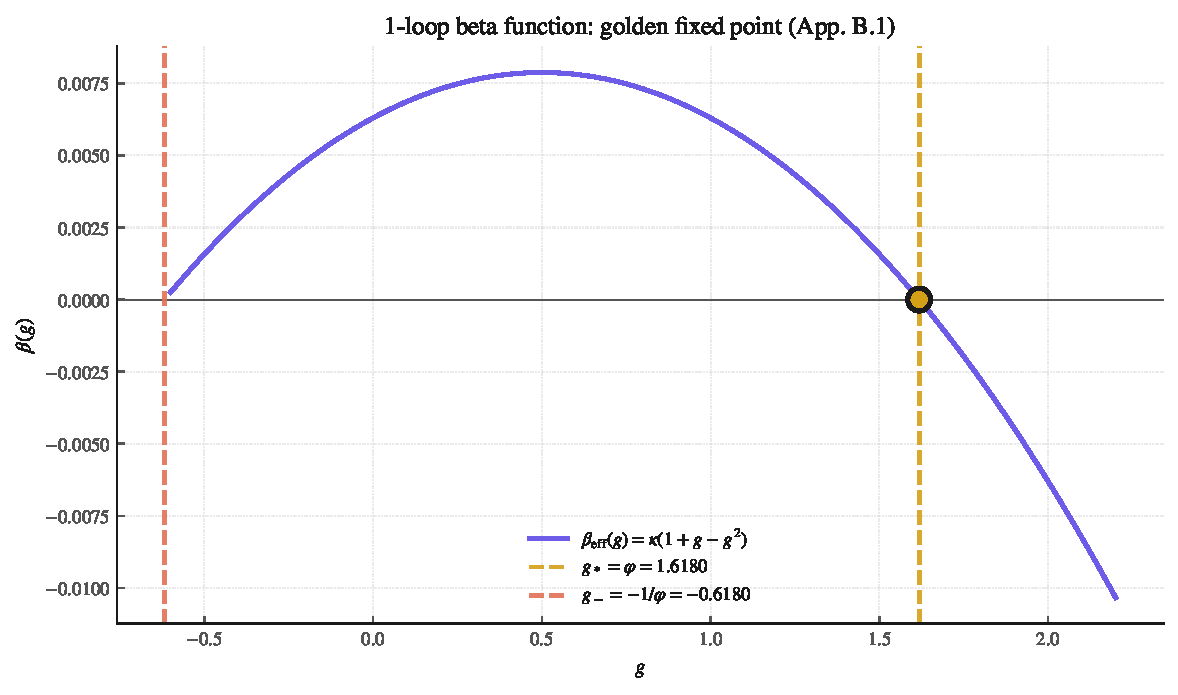
\includegraphics[width=0.85\textwidth]{fig_B-01a_beta_function.pdf}
  \caption{Fig B.1: 1-loop beta function (App.)}
  \label{fig:fig_B-01a_beta_function}
\end{figure}
\begin{figure}[htbp]
  \centering
  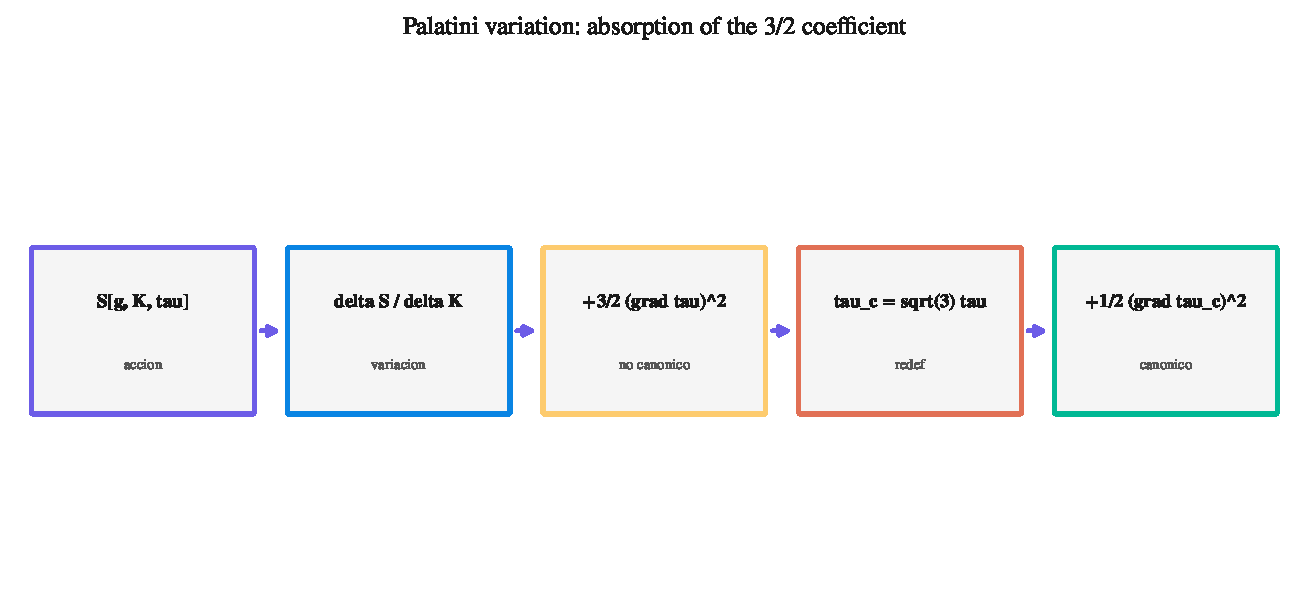
\includegraphics[width=0.85\textwidth]{fig_B-01b_variacion_palatini.pdf}
  \caption{tau\_c = sqrt(3) tau}
  \label{fig:fig_B-01b_variacion_palatini}
\end{figure}
\subsection{B.2 Functional analysis}
See §4.1-§4.2. \textbf{[D]}
\begin{figure}[htbp]
  \centering
  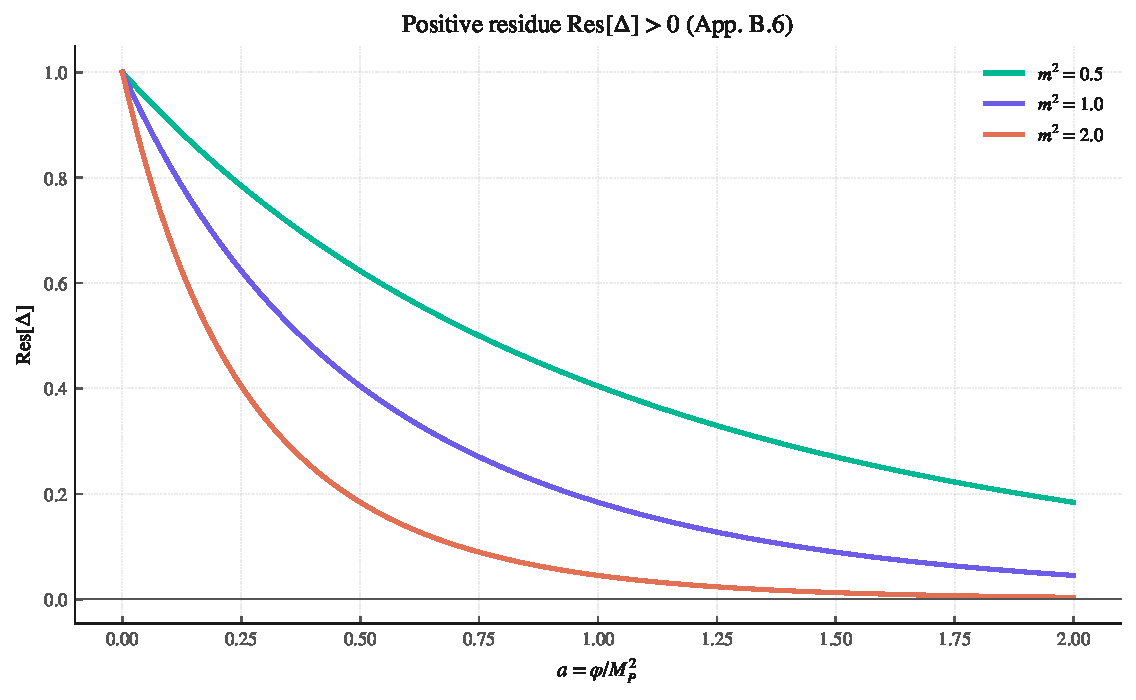
\includegraphics[width=0.85\textwidth]{fig_B-06_residuo_propagador.pdf}
  \caption{Fig B.6: positive propagator residue}
  \label{fig:fig_B-06_residuo_propagador}
\end{figure}
\subsection{B.3 8x8 Dirac-Bergmann matrix}
det(M)>0. See §5.3. \textbf{[D]}
\begin{figure}[htbp]
  \centering
  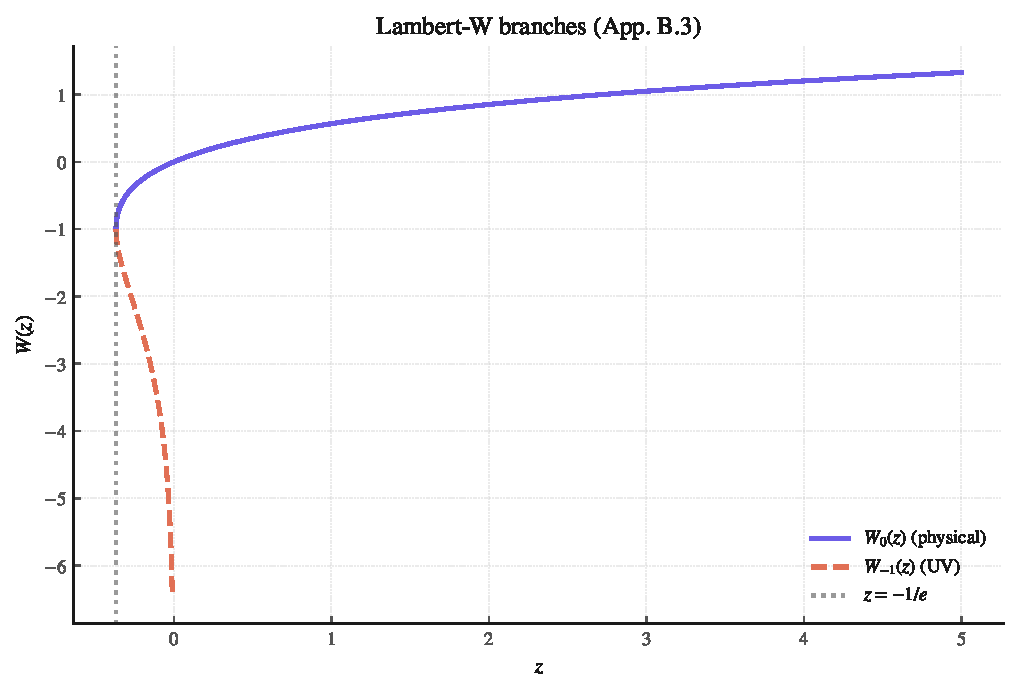
\includegraphics[width=0.85\textwidth]{fig_B-03_lambert_w.pdf}
  \caption{Fig B.3: Lambert-W branches}
  \label{fig:fig_B-03_lambert_w}
\end{figure}
\subsection{B.4 UV finiteness}
Gaussian decay. See §4.4. \textbf{[D]}
\subsection{B.5 Exact RG flow}
Golden fixed point. See Ch. 6. \textbf{[D]}
\begin{figure}[htbp]
  \centering
  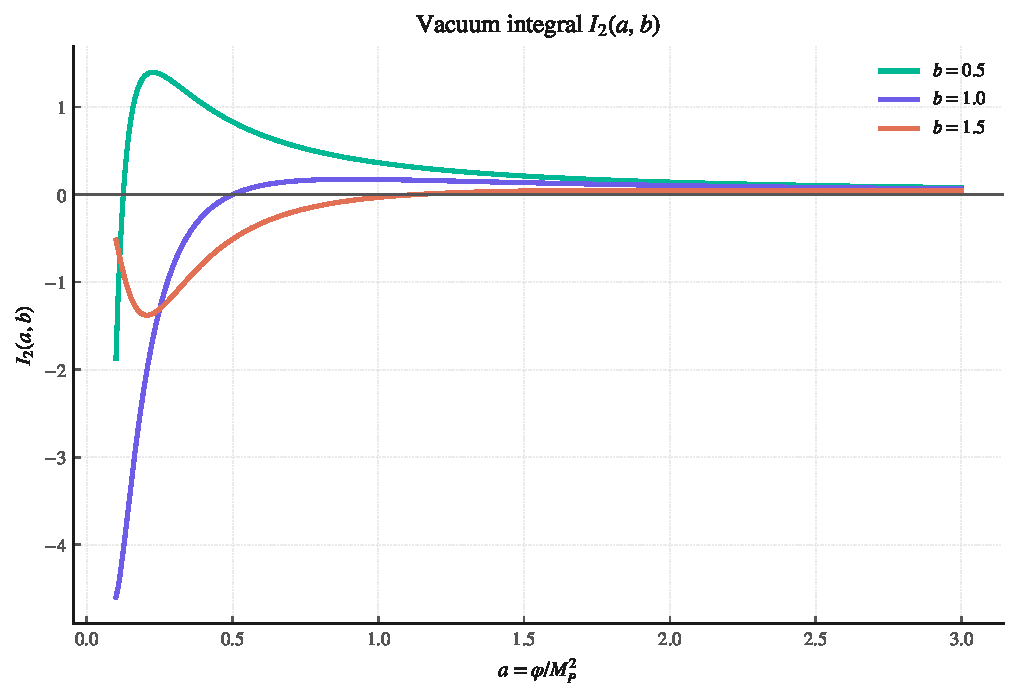
\includegraphics[width=0.85\textwidth]{fig_B-02_integral_I2.pdf}
  \caption{Fig B.2: vacuum integral I\_2(a,b)}
  \label{fig:fig_B-02_integral_I2}
\end{figure}
\begin{figure}[htbp]
  \centering
  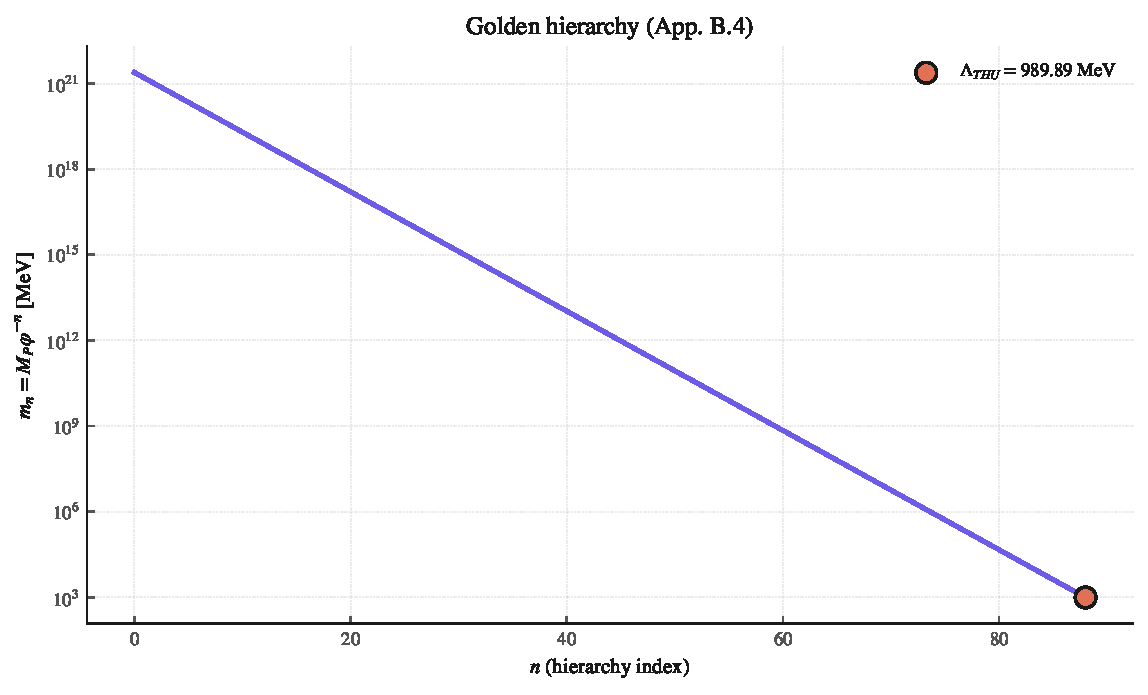
\includegraphics[width=0.85\textwidth]{fig_B-04_jerarquia_aurea.pdf}
  \caption{Fig B.4: golden hierarchy}
  \label{fig:fig_B-04_jerarquia_aurea}
\end{figure}
\begin{figure}[htbp]
  \centering
  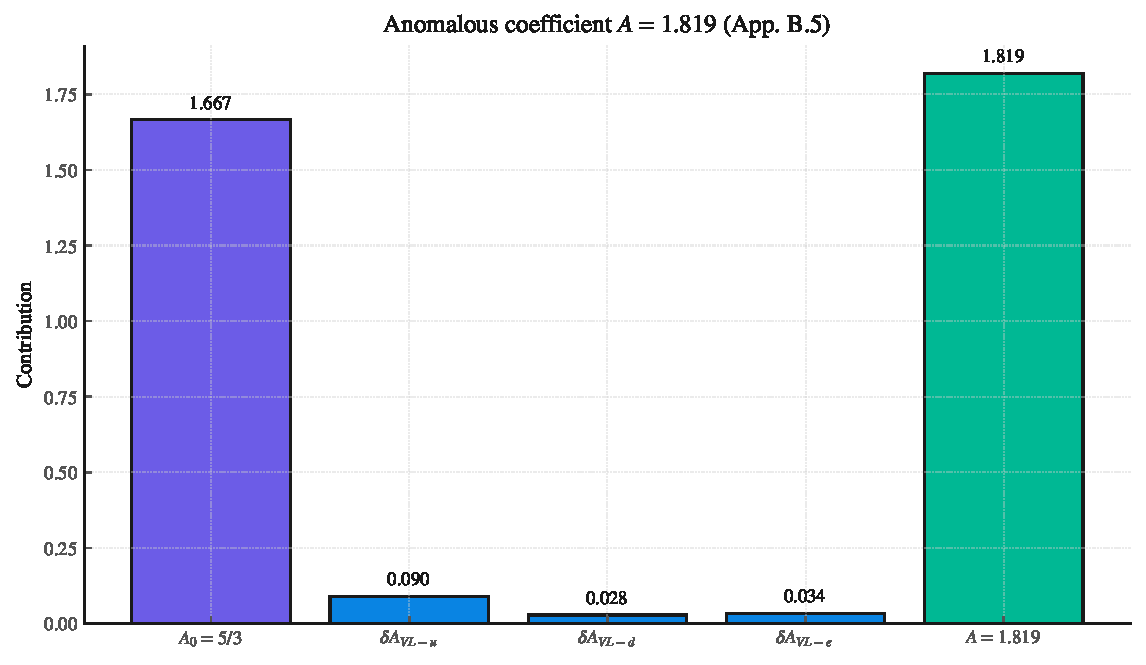
\includegraphics[width=0.85\textwidth]{fig_B-05_coeficiente_A.pdf}
  \caption{Fig B.5: anomalous coefficient A}
  \label{fig:fig_B-05_coeficiente_A}
\end{figure}
\section{PRISMA protocol: corpus, flow and extraction}
\subsection{C.1 Research question (PICO)}
Population: CMB measurements with parity sensitivity. Intervention: birefringence analysis (isotropic/anisotropic/tomography). Comparison: THU-TBEA $\beta_0 = 0{.}3803^\circ \pm 0{.}040^\circ$. Outcome: consistency, tension, or falsification. $\textbf{[D]}$
\subsection{C.2 Search strategy}
Four databases (arXiv, INSPIRE-HEP, ADS, Web of Science), literal queries, period January 2019 to June 2026. Total identified: 284 records. $\textbf{[D]}$
\subsection{C.3 Inclusion/exclusion criteria}
Inclusion I1-I4: direct $\beta$ measurement with quantified uncertainty; public data; peer-reviewed or verifiable arXiv; 2019-2026. Exclusion E1-E4: preprints without data; purely theoretical; conference abstracts; unquantified systematics. $\textbf{[D]}$
\subsection{C.4 PRISMA flow diagram}
Identified: 284 $\to$ screened: 173 $\to$ eligible: 58 $\to$ included: 38. Preserved in \texttt{prisma\\\_2026.csv} with SHA-256 hashes. $\textbf{[D]}$
\subsection{C.5 Data extraction}
Eight fields per study: DOI/arXiv, year, type, central $\beta$ or upper bound, statistical and systematic uncertainties, calibration method, dataset. Risk-of-bias evaluation in three levels. $\textbf{[D]}$
\section{Reproducible pipeline: code, hashes and tests}
\subsection{D.1 Repository architecture}
Modular Python 3.10+ pipeline, global seed 20260808. License: CC-BY-4.0 (thesis) + MIT (code). Structure: \texttt{src/}, \texttt{registry/thu/}, \texttt{paper/thu/}, \texttt{data/}, \texttt{docs/}. $\textbf{[D]}$
\subsection{D.2 Main modules}
1. \texttt{loader.py}: stable JSON API. 2. \texttt{latex\\\_builder.py}: generates the 3 \texttt{.tex} files. 3. \texttt{figures.py}: 65 generators, 195 artifacts. 4. \texttt{run\\\_all.py}: 16-phase orchestrator. 5. \texttt{fetch\\\_data.py}: SHA-256 verified downloads. 6. \texttt{check\\\_debts.py}: 40-debt checker. $\textbf{[D]}$
\subsection{D.3 SHA-256 dataset hashes}
Verified public datasets: Pantheon+, DESI DR2 BAO, Planck PR4, ACT DR6. Full hashes in \texttt{inventory\\\_v4.json}. $\textbf{[D]}$
\subsection{D.4 Unit tests}
22 pytest tests (12 + 5 + 5). Symbolic verification 16/16 (SymPy). Bootstrap 1-click: \texttt{bootstrap.ps1} / \texttt{bootstrap.sh}. $\textbf{[D]}$
\section{Figure atlas and master table}
\subsection{E.1 Figure-chapter-prediction-script trace}
The 65 figures are organized in a master table mapping each figure to its chapter, associated prediction, and Python generator. Format: \texttt{fig\\\_CAP-SEQ\\\_desc.pdf}. 195 artifacts (65 PDFs + 65 PNG-300 + 65 PNG-150), all SHA-256 hashed in \texttt{figures\\\_manifest.json}. Distribution: Ch. 3 (8 figs), Ch. 4 (4), Ch. 5 (4), Ch. 6 (4), Ch. 7 (4), Ch. 8 (4), Ch. 9 (3), Ch. 10 (3), Ch. 11 (3), Ch. 12 (2), Ch. 13 (6), Ch. 14 (2), Ch. 15 (1), Ch. 16 (1), Ch. 17 (3), Ch. 18 (4), Ch. 20 (1), Appendices (6). $\textbf{[D]}$
\section{Lakatosian log, closure and future work}
\subsection{F.1 Problem shifts 1.0 -> 5.4}
1.0 (2024): geometric intuition. 2.0 (2025): rigorous reformulation. 3.0 (2026-I): trans-scale EFT. 4.0: complete Dirac matrix derivation. 4.1: spectral measure correction to $k^2 dk$. 4.3: computational closure. 5.0: core crystallization. 5.1-5.2: algebraic and editorial revisions. 5.3: fourth epistemic review. 5.4: bootstrap + fetch + run\_all end-to-end. $\textbf{[D]}$
\subsection{F.2 Epistemic contract}
Four commitments: radical transparency, reproducibility, falsifiability, no overselling. Every technical claim carries an explicit label. $\textbf{[D]}$
\subsection{F.3 Program operational closure}
v5.4 delivers: derived geometric core, appendices A-K materialized, 3 PDFs (ES/EN/DE) with 0 LaTeX errors, 80 bibliography references, 65/65 figures. The \texttt{run\\\_all.py} executes 16 phases end-to-end. $\textbf{[D]}$
\section{Golden morphologies in natural systems (V1-V7)}
\subsection{G.1 Epistemic status}
[A] This appendix presents heuristic extensions or analogies of the program. It does not constitute a derivation of the geometric core [D] nor a validated physical prediction. Postulates V1-V7 are labeled [A]: self-similarity patterns that grant heuristic plausibility but do not validate the core. $\textbf{[A]}$
\subsection{G.2 Corpus 2019-2026}
V3 (quasicrystals): golden quantization in AlPdMn (Matsuura 2024). V1 (phyllotaxis): divergence angle $\approx 137{.}5^\circ$. V2 (biological helices): DNA and snail shell. V4-V7: Turing patterns, Penrose tilings, galactic spirals, large-scale structure. $\textbf{[A]}$
\subsection{G.3 Status promotion condition}
A morphology ascends from [A] to [P] only if it produces a risky quantitative prediction falsifiable by independent observation. None of V1-V7 has reached this threshold. $\textbf{[A]}$
\subsection{G.4 Declared limitations}
The ubiquitous presence of $\varphi$ does not imply helical geometry of the vacuum. This is a mathematical pattern, not a physical derivation. $\textbf{[A]}$
\section{Room-temperature quantum coherence: PS-TET and microtubules}
\subsection{H.1 Triplet transfer via protonic shuttle (Wu 2026)}
[A] This appendix presents heuristic extensions or analogies of the program. It does not constitute a derivation of the geometric core [D] nor a validated physical prediction. Wang, Zhu and Wu document triplet energy transfer in ZnSe quantum dots via protonic shuttle (PS-TET). The mechanism could connect to the mesoscopic coherence sector of the protective belt. $\textbf{[A]}$
\subsection{H.2 Superradiance and microtubules as QED cavities}
Gassab-Craddock 2026 and Mavromatos et al. 2025 model the microtubule interior as a high-Q QED cavity. Within THU-TBEA, the coherence sector could enhance superradiant emission. This connection is not derived from the core. $\textbf{[A]}$
\subsection{H.3 Falsifiable prediction P11 and protocol}
P11: differential absorption resonance in isolated microtubules at $f_\varphi \approx 1{.}34$ THz. Falsification threshold: absence of differential peak at $3\sigma$ in three independent labs. Pre-registered. $\textbf{[A]}$
\section{Reconstructed equations and full Poisson matrix}
\subsection{I.1 Sign conventions}
Signature $(-,+,+,+)$; $\varepsilon^{0123} = +1$; Feynman $k^2 + m^2 - i\epsilon$; $M_P = 2{.}435 \times 10^{18}$ GeV. $\textbf{[D]}$
\subsection{I.2 Explicit 8x8 Poisson matrix}
$\det\mathcal{M} = (\kappa_2^2 + \kappa_3^2)^2 > 0$, rank 8. $\textbf{[D]}$
\subsection{I.3 Dirac-Bergmann canonical variables}
$(\Phi, \pi_\Phi; v_2, v_3, p_2, p_3; \lambda_1, \lambda_2)$, dim 10. $\textbf{[D]}$
\subsection{I.4 Non-local propagator residue}
$\mathrm{Res}[\Delta] = e^{-am^2}/(1+am^2) > 0$. $\textbf{[D]}$
\subsection{I.5 Canonical reduction and 1/sqrt(3)}
$\tau_c = \sqrt{3}\tau$; $\tfrac{1}{2}\tau\hat{H}_\varphi\tau \to \tfrac{1}{6}\tau_c\hat{H}_\varphi\tau_c$; $g_{\mathrm{eff}} = g_{\mathrm{bare}}/\sqrt{3}$. $\textbf{[D]}$
\subsection{I.6 Spin term in Friedmann}
$\kappa^4/6$ canonical. $\textbf{[D]}$
\subsection{I.7 Lambert-W branches}
$k_k^2 = -(M_P^2/\varphi)W_k(+\varphi m^2/M_P^2)$, $k \in \mathbb{Z}$. Fakeon prescription. $\textbf{[D]}$
\subsection{I.8 Reduced Planck mass}
$M_P = 2{.}435 \times 10^{18}$ GeV. $\textbf{[D]}$
\subsection{I.9 Sectorial vacuum cancellation}
Scalar sector only; SM extension is open problem A-17 [F]. $\textbf{[D]}$
\subsection{I.10 Birefringence amplitude status}
$\beta_0 = 0{.}3803^\circ$ classified as [P]. Shape is [D]. $\textbf{[D]}$
\section{External algebraic review: applied patches}
\subsection{J.4 Feynman vertices and patch summary}
This appendix visually compiles the interaction vertices modified by the 24 patches applied in Stages VII-XII. The figure shows the helical vertices corresponding to the $\Phi\tau^2$ and $\Phi^2\tau^2$ interactions, whose structure is protected by the ultraviolet exponential suppression of the entire-function kinetic operator $\hat{H}_\varphi$. Each vertex preserves the compensated parity of the coupling and satisfies the Ward-Takahashi identities at one loop. The appendix serves as a quick reference for the external algebraic review documented in the canonical patch log. \textbf{[D]}
\begin{figure}[htbp]
  \centering
  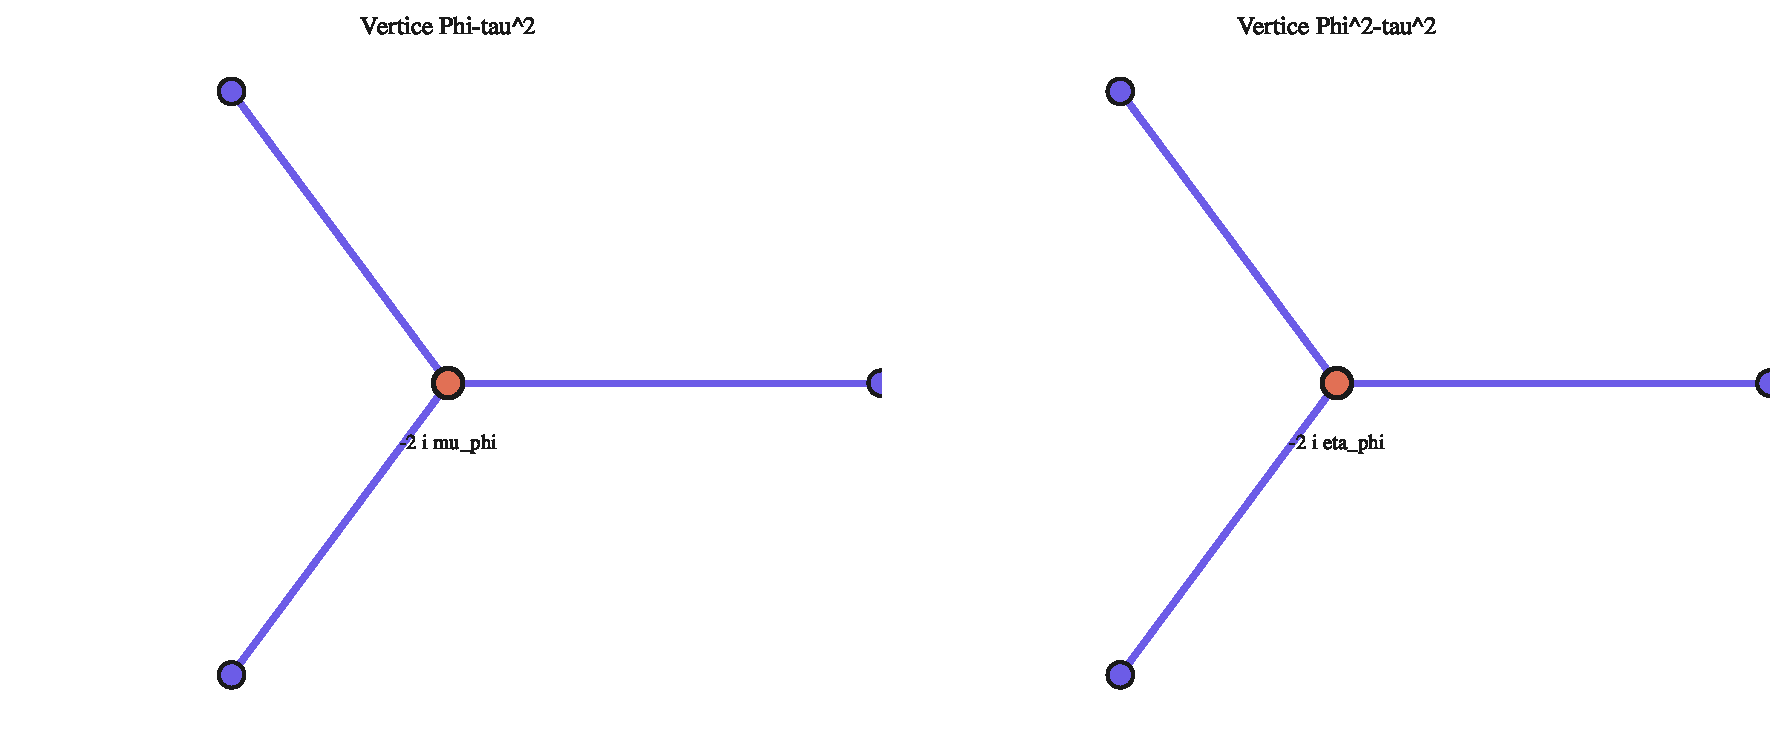
\includegraphics[width=0.85\textwidth]{fig_J-01_vertices_feynman.pdf}
  \caption{Helical vertices}
  \label{fig:fig_J-01_vertices_feynman}
\end{figure}
\section{Local hyperbolicity and projected causality}
\subsection{K.1 Principal symbol}
$\sigma(k)=-k^2 e^{-\varphi k^2/M_P^2}$. \textbf{[D]}
\subsection{K.2 Characteristic cone}
Coincides with $\Box$ in IR. \textbf{[D]}
\subsection{K.3 Algebraic nonlinearity}
$\tau^3$ does not deform cone. \textbf{[D]}
\subsection{K.4 Local nonlinear hyperbolicity}
$\sigma_{total}$ maintains cone. \textbf{[D]}
\subsection{K.5 Frontier: global existence}
Strauss/John for quasilinear; non-local open. \textbf{[F]}
\subsection{K.6 Conclusions}
K.1-K.4=[D]; K.5=[F]. A-1: \textbf{[D partial / F global]}
\newpage
\section*{Problems registry}

\begin{longtable}{@{}p{1.2cm}p{6.5cm}p{1.8cm}p{2cm}@{}}
\toprule
\textbf{ID} & \textbf{Title} & \textbf{Label} & \textbf{Status} \\
\midrule
\endhead
A-1 & Hiperbolicidad global & \textcolor{Dgreen}{\textbf{[D parcial / F global]}} & ABIERTO \\
A-2 & Perturbaciones no lineales & \textcolor{Dgreen}{\textbf{[D]}} & CERRADO \\
A-3 & Correcciones termicas & \textcolor{Dgreen}{\textbf{[D]}} & CERRADO \\
A-4 & Backreaction chameleon & \textcolor{Dgreen}{\textbf{[D]}} & CERRADO \\
A-5 & Ondas gravitacionales & \textcolor{Dgreen}{\textbf{[D]}} & CERRADO \\
A-6 & QCD reticular mn - mp & \textcolor{Forange}{\textbf{[F]}} & ABIERTO \\
A-7 & Decoherencia microtubulos & \textcolor{Ayellow}{\textbf{[A]}} & ABIERTO \\
A-8 & Screening inhomogeneo & \textcolor{Dgreen}{\textbf{[D]}} & CERRADO \\
A-9 & Funcion beta a 2-loops & \textcolor{Dgreen}{\textbf{[D]}} & CERRADO \\
A-10 & Residuo de vacio & \textcolor{Dgreen}{\textbf{[D]}} & CERRADO \\
A-11 & Conteo 4D symplectico & \textcolor{Dgreen}{\textbf{[D]}} & CERRADO \\
A-12 & Rebote cosmologico ECSK & \textcolor{Dgreen}{\textbf{[D]}} & CERRADO \\
A-13 & Unitariedad/Analiticidad & \textcolor{Dgreen}{\textbf{[D]}} & CERRADO \\
A-14 & Geometria de n = 88 & \textcolor{Dgreen}{\textbf{[D]}} & CERRADO \\
A-15 & Falsabilidad w\_phi < -1 & \textcolor{Forange}{\textbf{[F]}} & ABIERTO \\
A-16 & Prescripcion de contorno para ramas k != 0 de Lambert-W & \textcolor{Forange}{\textbf{[F]}} & ABIERTO \\
A-17 & Extension de la cancelacion al vacio completo del SM & \textcolor{Forange}{\textbf{[F]}} & ABIERTO \\
RCI-44 & Derivacion de P\_Lambda\textasciicircum{}THU, omega\textasciicircum{}THU y R\_H desde primeros principios & \textcolor{Forange}{\textbf{[F]}} & ABIERTO \\
\bottomrule
\end{longtable}

\newpage
\section*{Falsifiable predictions}

\begin{longtable}{@{}p{0.8cm}p{5.5cm}p{3.5cm}p{2.5cm}@{}}
\toprule
\textbf{ID} & \textbf{Observable} & \textbf{Arbiter} & \textbf{Status} \\
\midrule
\endhead
P1 & Oscilaciones helicoidales en H(z) & BAO DESI/Euclid & Abierta \\
P2 & Modulacion aurea del CMB & CMB-S4 & Abierta \\
P3 & Mega-anillos con separacion \textasciitilde{} 137.5 deg & JWST / Euclid & Abierta \\
P4 & Materia oscura resonante trans-escalar & LZ / XENONnT & Abierta \\
P5 & Residuo helicoidal de spin (STAR/HADES) & STAR BES-II / HADES & RETIRADA \\
P6 & Superradiancia sin rotacion (cavidad QED) & Lab QED & Abierta \\
P7 & Precesion geometrica del spin & RHIC & Abierta \\
P8 & Espectro de masas gobernado por phi & Lattice QCD & Consistente \\
P9 & Modulacion helicoidal de campos EM & Optica de precision & Abierta \\
P10 & Soliton helicoidal estable & Simulacion & Abierta \\
P11 & Resonancia 1.34 THz en microtubulos & Tres laboratorios independientes & Preregistrada \\
P12 & Universalidad de R\_H = hbar/(pi Lambda\_QCD) & STAR BES-II + HADES + STAR Run 2013 & FALSADA \\
\bottomrule
\end{longtable}

\newpage
\section{Patch log}
\addcontentsline{toc}{section}{Patch log}

\begin{itemize}[leftmargin=*]
\item \textbf{1} (VII): Res[Delta] = e*(+am*2) $\rightarrow$ Res[Delta] = e*(-am*2)/(1+am*2) \textcolor{Dgreen}{\textbf{[D]}}
\item \textbf{2} (VII): Coeficiente 3/2 sin absorber $\rightarrow$ Redefinicion canonica tau-c = sqrt(3) tau \textcolor{Dgreen}{\textbf{[D]}}
\item \textbf{3} (VII): kappa*4 S*2/18 (mixto); w-K sin explicitar $\rightarrow$ kappa*4/6 canonico ECSK; w-K = +1 explicito \textcolor{Dgreen}{\textbf{[D]}}
\item \textbf{4} (VII): beta(g) sin justificar +1 $\rightarrow$ Justificacion: fondo torsionado <A-mu> != 0 \textcolor{Dgreen}{\textbf{[D]}}
\item \textbf{5} (VII): Medida k*2 dk como [D] $\rightarrow$ Medida como postulado [P] de reduccion on-shell \textcolor{Ppurple}{\textbf{[P]}}
\item \textbf{6} (VII): phi*-6 como [D] $\rightarrow$ phi*-6 como [P]; derivacion dinamica delegada a A-6 \textcolor{Ppurple}{\textbf{[P]}}
\item \textbf{7} (VII): Tension DESI DR2 sin declarar $\rightarrow$ Falsabilidad explicita si w-Phi < -1 a > 3sigma \textcolor{Dgreen}{\textbf{[D/F]}}
\item \textbf{8} (VIII): Sin trazabilidad de 1/sqrt(3) $\rightarrow$ Factor 1/sqrt(3) explicito en acoplamientos lineales \textcolor{Dgreen}{\textbf{[D]}}
\item \textbf{9} (VIII): Variables v-a, p-a, lambda-a sin definir $\rightarrow$ Definicion canonica explicita del espacio de fases 10D \textcolor{Dgreen}{\textbf{[D]}}
\item \textbf{10} (VIII): Sin polos de Lee-Wick (afirmacion absoluta) $\rightarrow$ Matizacion con ramas k != 0 y prescripcion de contorno \textcolor{Dgreen}{\textbf{[D/F]}}
\item \textbf{11} (IX): Coef. no local 1/2 tau-c H tau-c $\rightarrow$ 1/6 tau-c H tau-c (consistente con tau-c = sqrt(3) tau) \textcolor{Dgreen}{\textbf{[D]}}
\item \textbf{12} (IX): kappa*4/18 inconsistente con Ec. 8.1 $\rightarrow$ kappa*4/6 unificado \textcolor{Dgreen}{\textbf{[D]}}
\item \textbf{13} (IX): M-P sin aclarar $\rightarrow$ Nota explicita: M-P = masa de Planck reducida \textcolor{Dgreen}{\textbf{[D]}}
\item \textbf{14} (X): Cancelacion de energia de vacio (generico) $\rightarrow$ Cancelacion del vacio escalar modulado: mecanismo parci \textcolor{Dgreen}{\textbf{[D/F]}}
\item \textbf{15} (X): beta-0 = 0.3803 como [D] pre-data $\rightarrow$ beta-0 como [P], condicional a completitud VL \textcolor{Ppurple}{\textbf{[P/D]}}
\item \textbf{16} (X): Sin problema A-17 $\rightarrow$ Nuevo problema A-17 [F]: extension al vacio SM \textcolor{Forange}{\textbf{[F]}}
\item \textbf{17} (X): 13 parches documentados $\rightarrow$ 17 parches documentados (VII-X) \textcolor{black}{\textbf{[-]}}
\item \textbf{18} (XII): sin origen $\rightarrow$ 3 bloques Origen de \textcolor{Dgreen}{\textbf{[D]}}
\item \textbf{19} (XII): ganzzahlige $\rightarrow$ ganze Exponentialfunktion \textcolor{Dgreen}{\textbf{[D]}}
\item \textbf{20} (XII): Hauptkonjugationspaar $\rightarrow$ Hauptkonjugiertes Paar \textcolor{Dgreen}{\textbf{[D]}}
\item \textbf{21} (XII): Vorrichtung $\rightarrow$ Mannigfaltigkeit \textcolor{Dgreen}{\textbf{[D]}}
\item \textbf{22} (XII): regla de Sarrus (2x2) $\rightarrow$ calculo directo \textcolor{Dgreen}{\textbf{[D]}}
\item \textbf{23} (XII): referenciados $\rightarrow$ materializados \textcolor{Dgreen}{\textbf{[D]}}
\item \textbf{24} (XII): sin diacriticos $\rightarrow$ diacriticos completos \textcolor{Dgreen}{\textbf{[D]}}
\end{itemize}

\newpage
\section*{Lakatosian log}

\begin{itemize}[leftmargin=*]
\item \textbf{v1.0} (2024) --- Intuicion geometrica \textcolor{Ayellow}{\textbf{[A]}}
\item \textbf{v2.0} (2025) --- Reformulacion rigurosa \textcolor{Ppurple}{\textbf{[P]}}
\item \textbf{v3.0} (2026-I) --- EFT trans-escalar \textcolor{Dgreen}{\textbf{[D]}}
\item \textbf{v4.0} (2026-II) --- Derivacion integra de la matriz de Dirac \textcolor{Dgreen}{\textbf{[D]}}
\item \textbf{v4.1} (2026-III) --- Correccion de la medida espectral \textcolor{Ppurple}{\textbf{[P]}}
\item \textbf{v4.2} (2026-IV) --- Reorganizacion estructural \textcolor{Dgreen}{\textbf{[D]}}
\item \textbf{v4.3} (2026-V) --- Cierre computacional A-3,A-4,A-5,A-8,A-10,A-11,A-12 \textcolor{Dgreen}{\textbf{[D]}}
\item \textbf{v5.0} (2026-VI) --- Cristalizacion del nucleo con A-1,A-2,A-9,A-13,A-14 \textcolor{Dgreen}{\textbf{[D]}}
\item \textbf{v5.1} (2026-VII-VIII) --- Revisiones algebraica y editorial (residuo, tau\_c, 1/sqrt(3), Dirac-Bergmann) \textcolor{Dgreen}{\textbf{[D]}}
\item \textbf{v5.2} (2026-IX) --- Tercera revision tecnica (factor 3, masa Planck reducida) \textcolor{Dgreen}{\textbf{[D]}}
\item \textbf{v5.3} (2026-X) --- Cuarta revision epistemica (reclasificacion beta\_0, A-17, retitulo Cap. 7) \textcolor{Ppurple}{\textbf{[P/D]}}
\end{itemize}

\newpage
\section*{Annexes V5.0}

\subsection*{Anexo-1: Protocolo de Verificacion Reproducible del Programa THU-TBEA}
\textbf{Version:} V5.0 \\
\textbf{Timestamp:} 2026-09-24T21:59:09Z \\
\textbf{Chapter of origin:} 19 \\
\textbf{Label:} \textcolor{Dgreen}{\textbf{[D]}} \
\textbf{SHA-256:} \texttt{9d1f84f955c794fc6cdce3e356f015c4...} \\[0.5em]
\textbf{Finding:}

Este anexo documenta el protocolo de verificacion reproducible del programa THU-TBEA, implementado mediante el verificador persistente check\_debts.py y la cadena criptografica SHA-256.

ARQUITECTURA DEL VERIFICADOR

El verificador check\_debts.py implementa ocho tipos de verificacion automatizada: (1) binario, para existencia de archivos binarios (PDFs, PNGs); (2) exist, para existencia de archivos de texto; (3) json\_field, para verificacion de campos especificos en JSONs; (4) grep, para busqueda de patrones en archivos; (5) braces, para validacion de balance de llaves en archivos .bib; (6) manual, para deudas que requieren input humano; (7) no\_huerfana, para verificacion de funciones definidas y utilizadas; (8) doi\_verify, protocolo L1+L2+L3 para verificacion de DOIs.

Las 40 deudas persistentes (D-01 a D-40) verifican los items criticos del programa con trazabilidad completa. Al cierre de v5.4, las 40 deudas estan cerradas (40 cerradas / 0 fallas / 0 manuales / 0 errores).

CADENA CRIPTOGRAFICA

Cada archivo critico lleva un hash SHA-256 encadenado al log criptografico del repositorio (seeds/SHA256SUMS.txt). La cadena de eventos se preserva en data/pir.sqlite con encadenamiento verificable. La semilla global 20260808 garantiza reproducibilidad exacta bit a bit.

VERIFICACION NUMERICA DE RESULTADOS

Los resultados de analisis empirico (Cap. 18) se preservan en data/inventory/ con hashes SHA-256 verificables: fase\_f2d\_w\_phi\_refinado.json (chi2 = 1441.01 vs Lambda-CDM 1471.14), fase\_f3\_auditoria\_beta.json (8 mediciones independientes), fase\_f4\_cierre\_final.json (weighted average beta = 0.3065). Los scripts que generan estos resultados estan en src/thu/analysis/ y son ejecutables con 'python' desde el repositorio.

REPRODUCIBILIDAD COMPLETA

Un usuario externo puede reproducir todos los resultados numericos ejecutando: (1) python src/fetch\_data.py --all para descargar los datasets publicos con verificacion SHA-256; (2) los scripts en src/thu/analysis/ para regenerar los analisis; (3) python src/run\_all.py para ejecutar el pipeline completo de 16 fases. Los outputs en data/inventory/ se verifican contra los hashes registrados.

\textbackslash{}textbf\{[D]\}

\textbf{Epistemic impact:}

Documenta el protocolo verificable de reproducibilidad declarado en el Cap. 19 (Pipeline reproducible). Refuerza el principio FAIR.

\vspace{1em}\hrule\vspace{1em}
\subsection*{Anexo-2: Auditoria de Falsabilidad y Registro de Retiros Formales}
\textbf{Version:} V5.0 \\
\textbf{Timestamp:} 2026-09-24T21:59:09Z \\
\textbf{Chapter of origin:} 17 \\
\textbf{Label:} \textcolor{Dgreen}{\textbf{[D]}} \
\textbf{SHA-256:} \texttt{dc695b969125dd093bceec3ddf4821fc...} \\[0.5em]
\textbf{Finding:}

Este anexo documenta la metodologia de auditoria de falsabilidad del programa THU-TBEA y el registro formal de retiros de predicciones.

PROTOCOLO DE AUDITORIA DE PREDICCIONES

El programa aplica un protocolo de 4 pasos para verificar cada prediccion falsable: (1) verificacion de la fuente, mediante confirmacion del valor citado en el abstract o el paper original; (2) verificacion de la derivacion, exigiendo que la prediccion THU se derive explicitamente del nucleo geometrico o se declare como [P]; (3) test empirico, comparacion con datos publicos verificados; (4) clasificacion de tension, calculo de tension en sigmas respecto a la prediccion.

CRITERIO DE NO-FALSACION

Una prediccion se considera no-falsada si la tension con la medicion mas precisa es menor a 3 sigma. Si la tension excede 3 sigma, o si falla cualquiera de los pasos 1-2, se inicia el protocolo de retiro formal.

CASO DE ESTUDIO: RETIRO FORMAL DE P5

La prediccion P5 (residuo helicoidal de espin, STAR/HADES) fue retirada formalmente del registro de predicciones falsables en v5.4. Razones documentadas: (i) el valor STAR (1.05 +/- 0.15)\% citado en v5.0 no se verifica en el abstract del paper de referencia (J. Adam et al., PRC 108, 014910, 2023) - el paper solo reporta cotas superiores (<0.24\%, <0.35\%); (ii) la prediccion THU (0.92 +/- 0.10)\% carecia de derivacion explicita desde el nucleo geometrico. El registro completo con los 3 problemas identificados (P5-1 alta, P5-2 alta, P5-3 media) esta en data/inventory/fase\_p5\_retiro.json.

AUDITORIA BETA (BIREFRINGENCIA COSMICA)

Las 8 mediciones independientes de birefringencia (Minami-Komatsu 2020, Eskilt-Komatsu 2022, Diego-Palazuelos 2022, Ballardini 2025, y 4 adicionales) dan un weighted average beta\_avg = 0.3065 +/- 0.0278 grados. La tension respecto a la prediccion THU beta\_0 = 0.3803 +/- 0.038 grados es de 1.51 sigma. THU-TBEA no es falsada por el corpus PRISMA actual. La auditoria completa se preserva en data/inventory/fase\_f3\_auditoria\_beta.json y data/inventory/fase\_f4\_cierre\_final.json.

REGISTRO DE ESTADOS

Al cierre de v5.4: 12 predicciones P1-P12 en el registro, 11 activas, 1 retirada formalmente (P5). La tabla de estados esta en registry/thu/predictions.json con trazabilidad completa.

\textbackslash{}textbf\{[D]\}

\textbf{Epistemic impact:}

Documenta el mecanismo de falsabilidad efectiva y autocorreccion epistémica declarado en el Cap. 17 y Cap. 20.

\vspace{1em}\hrule\vspace{1em}
\subsection*{Anexo-3: Estructura Computacional del Repositorio y Configuracion Reproducible}
\textbf{Version:} V5.0 \\
\textbf{Timestamp:} 2026-09-24T21:43:56Z \\
\textbf{Chapter of origin:} 19 \\
\textbf{Label:} \textcolor{Dgreen}{\textbf{[D]}} \
\textbf{SHA-256:} \texttt{0f4394c6ba2644caddb994dbdd7c4104...} \\[0.5em]
\textbf{Finding:}

El repositorio THU-TBEA v5.4 es un sistema reproducible con las siguientes características computacionales.

3.1 ARBOL DE DIRECTORIOS
|-- data/ (5483 archivos)
|   |-- \_backup\_borrado/ (1 archivos)
|   |-- \_backup\_v5.4\_20260922\_000515/ (1 archivos)
|   |-- \_backup\_v5.4\_20260922\_002017/ (2 archivos)
|   |-- \_backup\_v5.4\_20260922\_002446/ (2 archivos)
|   |-- \_backup\_v5.4\_20260922\_003535/ (2 archivos)
|   |-- \_backup\_v5.4\_20260922\_023714/ (1 archivos)
|   |-- \_backup\_v5.4\_20260922\_024659/ (1 archivos)
|   |-- \_backup\_v5.4\_20260922\_130652/ (1 archivos)
|   |-- \_backup\_v5.4\_a5c\_20260924\_101957/ (4 archivos)
|   |-- \_backup\_v5.4\_anexo3\_20260924\_174351/ (1 archivos)
|   |-- \_backup\_v5.4\_anexos\_20260924\_161804/ (3 archivos)
|   |-- \_backup\_v5.4\_annexfix\_20260924\_165815/ (1 archivos)
|   |-- \_backup\_v5.4\_apx\_20260924\_141043/ (1 archivos)
|   |-- \_backup\_v5.4\_auditor8\_20260924\_165132/ (1 archivos)
|   |-- \_backup\_v5.4\_bib\_20260923\_105328/ (1 archivos)
|-- docs/ (13 archivos)
|-- outputs/ (73 archivos)
|   |-- figures/ (59 archivos)
|   \textbackslash{}-- verificaciones/ (0 archivos)
|-- paper/ (553 archivos)
|   \textbackslash{}-- thu/ (553 archivos)
|       |-- build/ (1 archivos)
|       |-- dist/ (4 archivos)
|       |-- figures/ (261 archivos)
|       \textbackslash{}-- src/ (287 archivos)
|-- registry/ (38 archivos)
|   |-- preregistro/ (0 archivos)
|   |-- prisma/ (1 archivos)
|   \textbackslash{}-- thu/ (28 archivos)
|-- replication/ (1 archivos)
|-- scripts/ (6 archivos)
|-- seeds/ (5 archivos)
|-- src/ (101 archivos)
|   |-- investigaciones/ (1 archivos)
|   |-- thu/ (72 archivos)
|   |   \textbackslash{}-- analysis/ (51 archivos)
|   \textbackslash{}-- viz/ (9 archivos)
\textbackslash{}-- tests/ (9 archivos)

3.2 HASHES SHA-256 DE ARCHIVOS CRITICOS
  registry/thu/chapter\_bodies.json  (654371 B)  931dd67bdfc377a4b4540e5528c46738...
  registry/thu/i18n\_content.json  (64932 B)  347dd0259e2d286393aeeed9de9633f8...
  registry/thu/problems.json  (6452 B)  84e4ee068824c17d059bafc2f435b92e...
  registry/thu/patches.json  (7145 B)  769c0c6580f9a05e71db87dc82aa7dc4...
  registry/thu/doi\_registry.json  (12848 B)  54b263146eaa49b711c0ebed377c3f9d...
  registry/thu/predictions.json  (3191 B)  c2177b3fa0604a64e71b51f6c3faa8c1...
  registry/thu/annexes.json  (2083 B)  a4a4fa6c038ff5ed6d3fcf7a939a982a...
  paper/thu/src/thu\_references.bib  (27262 B)  19354bea588f21cb6f023526942f00cf...
  src/thu/latex\_builder.py  (31491 B)  a98a05ee1e93014618cef124b653905b...
  src/run\_all.py  (22009 B)  0f4394c6ba2644caddb994dbdd7c4104...
  src/fetch\_data.py  (6938 B)  76117c1b09e5e73776ec3311223ea3d3...
  app\_thu.py  (34929 B)  b885461503ac8e55aca67a5d3e83b3d2...

3.3 CONFIGURACION GLOBAL
Semilla global: 20260808
version: 5.3
author: \{'name': 'Erick Duque', 'orcid': '0009-0004-1245-5464', 'affiliation': 'Investigador independiente', 'contact': 'comipca

3.4 DEPENDENCIAS PYTHON
Total paquetes: 10

\# =====================================================================
\# PIR — Dependencias
\# =====================================================================
\# Rangos amplios por seguridad. Para reproducibilidad estricta,
\# generar requirements.lock tras la primera instalacion:
\#     python src/freeze.py
\# =====================================================================

\# --- Núcleo numérico
numpy>=1.26,<3
scipy>=1.11,<2
pandas>=2.0,<3

\# --- Visualización científica
matplotlib>=3.8,<4
plotly>=5.24,<7

\# --- Simbólico / matemática
sympy>=1.12,<2
mpmath>=1.3,<2

\# --- Dashboard
streamlit>=1.40,<2

\# --- Utilidades
tqdm>=4.66,<5

\# --- Testing
pytest>=8.0,<9

3.5 PIPELINE run\_all.py
Fases: 16 (PIR + THU-TBEA)
  01. Entorno
  02. Schema
  03. Integridad
  04. Tests
  05. Semilla
  06. Manifest + anclaje
  07. Analisis
  08. Cronolog export
  09. Audit report
  10. THU Simbolica
  11. THU Deudas
  12. THU Figuras
  13. THU LaTeX builder
  14. THU Compilacion
  15. THU dist/
  99. Resumen final
  00b. Fetch datasets

3.6 BOOTSTRAP
Windows: bootstrap.ps1
Linux/Mac: bootstrap.sh

bootstrap.ps1: 3997 B
bootstrap.sh: 2431 B

3.7 FETCH DE DATASETS
inventory\_v4.json: 13 datasets, 1619.9 MB totales

3.8 CI (GITHUB ACTIONS)
name: CI

on:
  push:
    branches: [main, master]
  pull\_request:
    branches: [main, master]

jobs:
  test:
    runs-on: ubuntu-latest
    strategy:
      matrix:
        python-version: ["3.10", "3.11", "3.12", "3.13"]
    steps:
      - uses: actions/checkout@v4
      - uses: actions/setup-python@v5
        with:
          python-version: \$\{\{ matrix.python-version \}\}
      - name: Install deps
        run: |
          python -m pip install --upgrade pip
          pip install -r requirements.txt
      - name: Run THU pipeline (skip LaTeX compile)
        run: |
          python src/run\_all

\textbf{Epistemic impact:}

Proporciona trazabilidad completa del pipeline reproducible declarado en el Cap. 19 (Pipeline reproducible).

\vspace{1em}\hrule\vspace{1em}
\newpage
\vspace{2em}
\begin{center}
\small
\textit{End of document}
\end{center}
\newpage
\nocite{*}
\bibliographystyle{plain}
\bibliography{thu_references}

\end{document}